% Options for packages loaded elsewhere
\PassOptionsToPackage{unicode}{hyperref}
\PassOptionsToPackage{hyphens}{url}
\PassOptionsToPackage{dvipsnames,svgnames,x11names}{xcolor}
%
\documentclass[
  letterpaper,
  DIV=11,
  numbers=noendperiod]{scrreprt}

\usepackage{amsmath,amssymb}
\usepackage{iftex}
\ifPDFTeX
  \usepackage[T1]{fontenc}
  \usepackage[utf8]{inputenc}
  \usepackage{textcomp} % provide euro and other symbols
\else % if luatex or xetex
  \usepackage{unicode-math}
  \defaultfontfeatures{Scale=MatchLowercase}
  \defaultfontfeatures[\rmfamily]{Ligatures=TeX,Scale=1}
\fi
\usepackage{lmodern}
\ifPDFTeX\else  
    % xetex/luatex font selection
\fi
% Use upquote if available, for straight quotes in verbatim environments
\IfFileExists{upquote.sty}{\usepackage{upquote}}{}
\IfFileExists{microtype.sty}{% use microtype if available
  \usepackage[]{microtype}
  \UseMicrotypeSet[protrusion]{basicmath} % disable protrusion for tt fonts
}{}
\makeatletter
\@ifundefined{KOMAClassName}{% if non-KOMA class
  \IfFileExists{parskip.sty}{%
    \usepackage{parskip}
  }{% else
    \setlength{\parindent}{0pt}
    \setlength{\parskip}{6pt plus 2pt minus 1pt}}
}{% if KOMA class
  \KOMAoptions{parskip=half}}
\makeatother
\usepackage{xcolor}
\setlength{\emergencystretch}{3em} % prevent overfull lines
\setcounter{secnumdepth}{5}
% Make \paragraph and \subparagraph free-standing
\ifx\paragraph\undefined\else
  \let\oldparagraph\paragraph
  \renewcommand{\paragraph}[1]{\oldparagraph{#1}\mbox{}}
\fi
\ifx\subparagraph\undefined\else
  \let\oldsubparagraph\subparagraph
  \renewcommand{\subparagraph}[1]{\oldsubparagraph{#1}\mbox{}}
\fi

\usepackage{color}
\usepackage{fancyvrb}
\newcommand{\VerbBar}{|}
\newcommand{\VERB}{\Verb[commandchars=\\\{\}]}
\DefineVerbatimEnvironment{Highlighting}{Verbatim}{commandchars=\\\{\}}
% Add ',fontsize=\small' for more characters per line
\usepackage{framed}
\definecolor{shadecolor}{RGB}{241,243,245}
\newenvironment{Shaded}{\begin{snugshade}}{\end{snugshade}}
\newcommand{\AlertTok}[1]{\textcolor[rgb]{0.68,0.00,0.00}{#1}}
\newcommand{\AnnotationTok}[1]{\textcolor[rgb]{0.37,0.37,0.37}{#1}}
\newcommand{\AttributeTok}[1]{\textcolor[rgb]{0.40,0.45,0.13}{#1}}
\newcommand{\BaseNTok}[1]{\textcolor[rgb]{0.68,0.00,0.00}{#1}}
\newcommand{\BuiltInTok}[1]{\textcolor[rgb]{0.00,0.23,0.31}{#1}}
\newcommand{\CharTok}[1]{\textcolor[rgb]{0.13,0.47,0.30}{#1}}
\newcommand{\CommentTok}[1]{\textcolor[rgb]{0.37,0.37,0.37}{#1}}
\newcommand{\CommentVarTok}[1]{\textcolor[rgb]{0.37,0.37,0.37}{\textit{#1}}}
\newcommand{\ConstantTok}[1]{\textcolor[rgb]{0.56,0.35,0.01}{#1}}
\newcommand{\ControlFlowTok}[1]{\textcolor[rgb]{0.00,0.23,0.31}{#1}}
\newcommand{\DataTypeTok}[1]{\textcolor[rgb]{0.68,0.00,0.00}{#1}}
\newcommand{\DecValTok}[1]{\textcolor[rgb]{0.68,0.00,0.00}{#1}}
\newcommand{\DocumentationTok}[1]{\textcolor[rgb]{0.37,0.37,0.37}{\textit{#1}}}
\newcommand{\ErrorTok}[1]{\textcolor[rgb]{0.68,0.00,0.00}{#1}}
\newcommand{\ExtensionTok}[1]{\textcolor[rgb]{0.00,0.23,0.31}{#1}}
\newcommand{\FloatTok}[1]{\textcolor[rgb]{0.68,0.00,0.00}{#1}}
\newcommand{\FunctionTok}[1]{\textcolor[rgb]{0.28,0.35,0.67}{#1}}
\newcommand{\ImportTok}[1]{\textcolor[rgb]{0.00,0.46,0.62}{#1}}
\newcommand{\InformationTok}[1]{\textcolor[rgb]{0.37,0.37,0.37}{#1}}
\newcommand{\KeywordTok}[1]{\textcolor[rgb]{0.00,0.23,0.31}{#1}}
\newcommand{\NormalTok}[1]{\textcolor[rgb]{0.00,0.23,0.31}{#1}}
\newcommand{\OperatorTok}[1]{\textcolor[rgb]{0.37,0.37,0.37}{#1}}
\newcommand{\OtherTok}[1]{\textcolor[rgb]{0.00,0.23,0.31}{#1}}
\newcommand{\PreprocessorTok}[1]{\textcolor[rgb]{0.68,0.00,0.00}{#1}}
\newcommand{\RegionMarkerTok}[1]{\textcolor[rgb]{0.00,0.23,0.31}{#1}}
\newcommand{\SpecialCharTok}[1]{\textcolor[rgb]{0.37,0.37,0.37}{#1}}
\newcommand{\SpecialStringTok}[1]{\textcolor[rgb]{0.13,0.47,0.30}{#1}}
\newcommand{\StringTok}[1]{\textcolor[rgb]{0.13,0.47,0.30}{#1}}
\newcommand{\VariableTok}[1]{\textcolor[rgb]{0.07,0.07,0.07}{#1}}
\newcommand{\VerbatimStringTok}[1]{\textcolor[rgb]{0.13,0.47,0.30}{#1}}
\newcommand{\WarningTok}[1]{\textcolor[rgb]{0.37,0.37,0.37}{\textit{#1}}}

\providecommand{\tightlist}{%
  \setlength{\itemsep}{0pt}\setlength{\parskip}{0pt}}\usepackage{longtable,booktabs,array}
\usepackage{calc} % for calculating minipage widths
% Correct order of tables after \paragraph or \subparagraph
\usepackage{etoolbox}
\makeatletter
\patchcmd\longtable{\par}{\if@noskipsec\mbox{}\fi\par}{}{}
\makeatother
% Allow footnotes in longtable head/foot
\IfFileExists{footnotehyper.sty}{\usepackage{footnotehyper}}{\usepackage{footnote}}
\makesavenoteenv{longtable}
\usepackage{graphicx}
\makeatletter
\def\maxwidth{\ifdim\Gin@nat@width>\linewidth\linewidth\else\Gin@nat@width\fi}
\def\maxheight{\ifdim\Gin@nat@height>\textheight\textheight\else\Gin@nat@height\fi}
\makeatother
% Scale images if necessary, so that they will not overflow the page
% margins by default, and it is still possible to overwrite the defaults
% using explicit options in \includegraphics[width, height, ...]{}
\setkeys{Gin}{width=\maxwidth,height=\maxheight,keepaspectratio}
% Set default figure placement to htbp
\makeatletter
\def\fps@figure{htbp}
\makeatother
\newlength{\cslhangindent}
\setlength{\cslhangindent}{1.5em}
\newlength{\csllabelwidth}
\setlength{\csllabelwidth}{3em}
\newlength{\cslentryspacingunit} % times entry-spacing
\setlength{\cslentryspacingunit}{\parskip}
\newenvironment{CSLReferences}[2] % #1 hanging-ident, #2 entry spacing
 {% don't indent paragraphs
  \setlength{\parindent}{0pt}
  % turn on hanging indent if param 1 is 1
  \ifodd #1
  \let\oldpar\par
  \def\par{\hangindent=\cslhangindent\oldpar}
  \fi
  % set entry spacing
  \setlength{\parskip}{#2\cslentryspacingunit}
 }%
 {}
\usepackage{calc}
\newcommand{\CSLBlock}[1]{#1\hfill\break}
\newcommand{\CSLLeftMargin}[1]{\parbox[t]{\csllabelwidth}{#1}}
\newcommand{\CSLRightInline}[1]{\parbox[t]{\linewidth - \csllabelwidth}{#1}\break}
\newcommand{\CSLIndent}[1]{\hspace{\cslhangindent}#1}

\KOMAoption{captions}{tableheading}
\makeatletter
\@ifpackageloaded{tcolorbox}{}{\usepackage[skins,breakable]{tcolorbox}}
\@ifpackageloaded{fontawesome5}{}{\usepackage{fontawesome5}}
\definecolor{quarto-callout-color}{HTML}{909090}
\definecolor{quarto-callout-note-color}{HTML}{0758E5}
\definecolor{quarto-callout-important-color}{HTML}{CC1914}
\definecolor{quarto-callout-warning-color}{HTML}{EB9113}
\definecolor{quarto-callout-tip-color}{HTML}{00A047}
\definecolor{quarto-callout-caution-color}{HTML}{FC5300}
\definecolor{quarto-callout-color-frame}{HTML}{acacac}
\definecolor{quarto-callout-note-color-frame}{HTML}{4582ec}
\definecolor{quarto-callout-important-color-frame}{HTML}{d9534f}
\definecolor{quarto-callout-warning-color-frame}{HTML}{f0ad4e}
\definecolor{quarto-callout-tip-color-frame}{HTML}{02b875}
\definecolor{quarto-callout-caution-color-frame}{HTML}{fd7e14}
\makeatother
\makeatletter
\makeatother
\makeatletter
\@ifpackageloaded{bookmark}{}{\usepackage{bookmark}}
\makeatother
\makeatletter
\@ifpackageloaded{caption}{}{\usepackage{caption}}
\AtBeginDocument{%
\ifdefined\contentsname
  \renewcommand*\contentsname{Table of contents}
\else
  \newcommand\contentsname{Table of contents}
\fi
\ifdefined\listfigurename
  \renewcommand*\listfigurename{List of Figures}
\else
  \newcommand\listfigurename{List of Figures}
\fi
\ifdefined\listtablename
  \renewcommand*\listtablename{List of Tables}
\else
  \newcommand\listtablename{List of Tables}
\fi
\ifdefined\figurename
  \renewcommand*\figurename{Figure}
\else
  \newcommand\figurename{Figure}
\fi
\ifdefined\tablename
  \renewcommand*\tablename{Table}
\else
  \newcommand\tablename{Table}
\fi
}
\@ifpackageloaded{float}{}{\usepackage{float}}
\floatstyle{ruled}
\@ifundefined{c@chapter}{\newfloat{codelisting}{h}{lop}}{\newfloat{codelisting}{h}{lop}[chapter]}
\floatname{codelisting}{Listing}
\newcommand*\listoflistings{\listof{codelisting}{List of Listings}}
\makeatother
\makeatletter
\@ifpackageloaded{caption}{}{\usepackage{caption}}
\@ifpackageloaded{subcaption}{}{\usepackage{subcaption}}
\makeatother
\makeatletter
\@ifpackageloaded{tcolorbox}{}{\usepackage[skins,breakable]{tcolorbox}}
\makeatother
\makeatletter
\@ifundefined{shadecolor}{\definecolor{shadecolor}{rgb}{.97, .97, .97}}
\makeatother
\makeatletter
\makeatother
\makeatletter
\makeatother
\ifLuaTeX
  \usepackage{selnolig}  % disable illegal ligatures
\fi
\IfFileExists{bookmark.sty}{\usepackage{bookmark}}{\usepackage{hyperref}}
\IfFileExists{xurl.sty}{\usepackage{xurl}}{} % add URL line breaks if available
\urlstyle{same} % disable monospaced font for URLs
\hypersetup{
  pdftitle={Geodata \& Spatial Regression},
  pdfauthor={Tobias Rüttenauer},
  colorlinks=true,
  linkcolor={blue},
  filecolor={Maroon},
  citecolor={Blue},
  urlcolor={Blue},
  pdfcreator={LaTeX via pandoc}}

\title{Geodata \& Spatial Regression}
\author{Tobias Rüttenauer}
\date{2024-01-07}

\begin{document}
\maketitle
\ifdefined\Shaded\renewenvironment{Shaded}{\begin{tcolorbox}[frame hidden, sharp corners, borderline west={3pt}{0pt}{shadecolor}, breakable, interior hidden, boxrule=0pt, enhanced]}{\end{tcolorbox}}\fi

\renewcommand*\contentsname{Table of contents}
{
\hypersetup{linkcolor=}
\setcounter{tocdepth}{2}
\tableofcontents
}
\bookmarksetup{startatroot}

\hypertarget{introduction}{%
\chapter*{Introduction}\label{introduction}}
\addcontentsline{toc}{chapter}{Introduction}

\markboth{Introduction}{Introduction}

This course material is designed for the 3-days GESIS workshop on
geodata and spatial regression analysis. Rüttenauer (2024) provides a
handbook chapter accompanying these workshop materials.

In recent years, more and more spatial data has become available,
providing the possibility to combine otherwise unrelated data, such as
social, economic, and environmental data. This also opens up the
possibility of analysing spatial patterns and processes (e.g., spillover
effects or diffusion).

Many social science research questions are spatially dependent such as
voting outcomes, housing prices, labour markets, protest behaviour, or
migration decisions. Observing an event in one region or neighbourhood
increases the likelihood that we observe similar processes in proximate
areas. As Tobler's first law of geography puts it: ``Everything is
related to everything else, but near things are more related than
distant things''. This dependence can stem from spatial contagion,
spatial spillovers, or common confounders. Therefore, basic assumptions
of standard regression models are violated when analysing spatial data.
However, more importantly, spatial processes are interesting for their
own sake. Spatial regression models can detect spatial dependence and
explicitly model spatial relations, identifying spatial clustering,
spillovers or diffusion processes.

The main objective of the course is the theoretical understanding and
practical application of spatial regression models. This course will
first give an overview on how to perform common spatial operations using
spatial information, such as aggregating spatial units, calculating
distances, merging spatial data as well as visualizing them. The course
will further focus on the analysis of geographic data and the
application of spatial regression techniques to model and analyse
spatial processes, and furthermore, the course addresses several methods
for defining spatial relationships, detecting and diagnosing spatial
dependence and autocorrelation. Finally, we will discuss various spatial
regression techniques to model processes, clarify the assumptions of
these models, and show how they differ in their applications and
interpretations.

The field has developed very quickly over the past few years, and
\emph{R} now provides a rich set of packages for various spatial data
operations. For a more in-depth introduction into spatial data analysis
in \emph{R}, have a look into the materials references below.

The material introduces the use of geographical information to connect
and analyze different spatial data sources very briefly. This
introduction is limited to the fundamentals of using geographical
information in \emph{R}. \href{https://stefanjuenger.github.io/}{Stefan
Jünger} \&
\href{https://www.gesis.org/institut/mitarbeitendenverzeichnis/person/Anne-Kathrin.Stroppe}{Anne-Kathrin
Stroppe} have provided a comprehensive
\href{https://github.com/StefanJuenger/gesis-workshop-geospatial-techniques-R-2024}{GESIS
workshop on geospatial techniques in R}. The focus of this workshop will
be on techniques for spatial data analysis, such as spatial regression
models.

\hypertarget{schedule}{%
\section*{Schedule}\label{schedule}}
\addcontentsline{toc}{section}{Schedule}

\markright{Schedule}

\begin{longtable}[]{@{}ll@{}}
\toprule\noalign{}
Day 1 & Working with Spatial Data \\
\midrule\noalign{}
\endhead
\bottomrule\noalign{}
\endlastfoot
10:00 - 11:30 & Refresher on R as GIS \\
& Coffee break \\
11:45 - 13:00 & Spatial Data Manipulation \& Visualization \\
& Lunch break \\
14:00 - 15:30 & Defining Spatial Relationships (W) \\
& Coffee break \\
15:45 - 17:15 & Lab Exercises in R \\
\end{longtable}

\begin{longtable}[]{@{}ll@{}}
\toprule\noalign{}
Day 2 & Spatial Regression Models I \\
\midrule\noalign{}
\endhead
\bottomrule\noalign{}
\endlastfoot
10:00 - 11:30 & Detecting Spatial Dependence \\
& Coffee break \\
11:45 - 13:00 & Spatial Regression Models: Theory \\
& Lunch break \\
14:00 - 15:30 & Estimating Spatial Regression Models \\
& Coffee break \\
15:45 - 17:15 & Lab Exercises in R \\
\end{longtable}

\begin{longtable}[]{@{}ll@{}}
\toprule\noalign{}
Day 3 & Spatial Regression Models II \\
\midrule\noalign{}
\endhead
\bottomrule\noalign{}
\endlastfoot
10:00 - 11:30 & Interpreting Results: Spatial Impacts \\
& Coffee break \\
11:45 - 13:00 & Comparing and Selecting Models \\
& Lunch break \\
14:00 - 15:30 & Lab Exercises in R \\
& Coffee break \\
15:45 - 17:15 & Other Models \\
\end{longtable}

\hypertarget{some-useful-packages}{%
\section*{Some useful packages}\label{some-useful-packages}}
\addcontentsline{toc}{section}{Some useful packages}

\markright{Some useful packages}

By now, \emph{R} provides a lot of functionalities for GIS applications
and spatial econometrics, and further extensions. There are lots of
packages providing a huge variety of spatial functionalities and methods
(see e.g. R. Bivand, Millo, and Piras 2021). Important packages for
fundamental spatial operations are:

\begin{itemize}
\item
  Spatial data workhorses:
  \href{https://cran.r-project.org/web/packages/sf/index.html}{sf}
  (Pebesma 2018) and
  \href{https://cran.r-project.org/web/packages/terra/index.html}{terra}
\item
  Visualization:
  \href{https://cran.r-project.org/web/packages/mapview/index.html}{mapview}
  (Appelhans et al. 2021) and
  \href{https://cran.r-project.org/web/packages/tmap/index.html}{tmap}
  (Tennekes 2018)
\item
  Spatial weights and other relations:
  \href{https://cran.r-project.org/web/packages/stars/index.html}{spdep}
  (R. S. Bivand and Rudel 2018)
\item
  Spatial interpolation and kriging:
  \href{https://cran.r-project.org/web/packages/gstat/index.html}{gstat}
  (Gräler, Pebesma, and Heuvelink 2016)
\item
  Spatial regression models:
  \href{https://cran.r-project.org/web/packages/spatialreg/index.html}{spatialreg}
  and
  \href{https://cran.r-project.org/web/packages/sphet/index.html}{sphet}
  (R. Bivand and Piras 2015)
\item
  The packages have constantly developed over the past years, and older
  packages such as rgdal, rgeos, and sp are currently retiring
  (\href{https://geocompx.org/post/2023/rgdal-retirement/}{Blog post})
\end{itemize}

\hypertarget{further-readings}{%
\section*{Further Readings}\label{further-readings}}
\addcontentsline{toc}{section}{Further Readings}

\markright{Further Readings}

\begin{itemize}
\item
  Great up-to-date introduction to spatial R: Lovelace, Nowosad, and
  Muenchow (2019), \href{https://geocompr.robinlovelace.net/}{updated
  version available online}
\item
  Great open-science book on
  \href{https://www.r-spatial.org/book}{Spatial Data Science} Pebesma
  and Bivand (2023)
\item
  Comprehensive introduction to spatial econometrics: LeSage and Pace
  (2009)
\item
  Relative intuitive introduction to spatial econometrics: Ward and
  Gleditsch (2008)
\item
  Article-length introductions to spatial econometrics: Elhorst (2012),
  Halleck Vega and Elhorst (2015), LeSage (2014a), Rüttenauer (2024),
  and Rüttenauer (2022)
\end{itemize}

\hypertarget{course-materials}{%
\section*{Course materials}\label{course-materials}}
\addcontentsline{toc}{section}{Course materials}

\markright{Course materials}

\begin{itemize}
\item
  I highly recommend the great Introduction to Geospatial Techniques for
  Social Scientists in R including, see
  \href{https://stefanjuenger.github.io/}{Stefan Jünger} \&
  \href{https://www.gesis.org/institut/mitarbeitendenverzeichnis/person/Anne-Kathrin.Stroppe}{Anne-Kathrin
  Stroppe}'s
  \href{https://github.com/StefanJuenger/gesis-workshop-geospatial-techniques-R-2023}{GESIS
  workshop materials}. Nice materials on GIS, spatial operations and
  spatial data visualisation!
\item
  For those looking for a more in-depth introduction, I highly recommend
  Roger Bivand's course on Spatial Data Analysis:
  \href{https://www.youtube.com/watch?v=KkIbg50Pa0I\&list=PLXUoTpMa_9s10NVk4dBQljNOaOXAOhcE0}{Youtube
  recordings}, \href{https://rsbivand.github.io/ECS530_h19/}{Course
  Materials}
\item
  I've learned most of what I know about spatial econometrics from
  \href{http://www.scottjcook.net/}{Scott J. Cook} and his workshop on
  Spatial Econometrics at the
  \href{https://essexsummerschool.com/summer-school-facts/courses/ess-2023-course-list/}{Essex
  Summer school}.
\end{itemize}

\bookmarksetup{startatroot}

\hypertarget{refresher}{%
\chapter{Refresher}\label{refresher}}

\hypertarget{required-packages}{%
\subsection*{Required packages}\label{required-packages}}
\addcontentsline{toc}{subsection}{Required packages}

\begin{Shaded}
\begin{Highlighting}[]
\NormalTok{pkgs }\OtherTok{\textless{}{-}} \FunctionTok{c}\NormalTok{(}\StringTok{"sf"}\NormalTok{, }\StringTok{"gstat"}\NormalTok{, }\StringTok{"mapview"}\NormalTok{, }\StringTok{"nngeo"}\NormalTok{, }\StringTok{"rnaturalearth"}\NormalTok{, }\StringTok{"dplyr"}\NormalTok{,}
          \StringTok{"nomisr"}\NormalTok{, }\StringTok{"osmdata"}\NormalTok{, }\StringTok{"tidyr"}\NormalTok{, }\StringTok{"texreg"}\NormalTok{) }
\FunctionTok{lapply}\NormalTok{(pkgs, require, }\AttributeTok{character.only =} \ConstantTok{TRUE}\NormalTok{)}
\end{Highlighting}
\end{Shaded}

\hypertarget{session-info}{%
\subsection*{Session info}\label{session-info}}
\addcontentsline{toc}{subsection}{Session info}

\begin{Shaded}
\begin{Highlighting}[]
\FunctionTok{sessionInfo}\NormalTok{()}
\end{Highlighting}
\end{Shaded}

\begin{verbatim}
R version 4.4.1 (2024-06-14 ucrt)
Platform: x86_64-w64-mingw32/x64
Running under: Windows 11 x64 (build 22631)

Matrix products: default


locale:
[1] LC_COLLATE=English_United Kingdom.utf8 
[2] LC_CTYPE=English_United Kingdom.utf8   
[3] LC_MONETARY=English_United Kingdom.utf8
[4] LC_NUMERIC=C                           
[5] LC_TIME=English_United Kingdom.utf8    

time zone: Europe/Berlin
tzcode source: internal

attached base packages:
[1] stats     graphics  grDevices utils     datasets  methods   base     

other attached packages:
 [1] texreg_1.39.3       tidyr_1.3.1         osmdata_0.2.5      
 [4] nomisr_0.4.7        dplyr_1.1.4         rnaturalearth_1.0.1
 [7] nngeo_0.4.8         mapview_2.11.2      gstat_2.1-1        
[10] sf_1.0-16          

loaded via a namespace (and not attached):
 [1] xfun_0.45          raster_3.6-26      htmlwidgets_1.6.4  lattice_0.22-6    
 [5] vctrs_0.6.5        tools_4.4.1        crosstalk_1.2.1    generics_0.1.3    
 [9] stats4_4.4.1       tibble_3.2.1       proxy_0.4-27       spacetime_1.3-1   
[13] fansi_1.0.6        xts_0.14.0         pkgconfig_2.0.3    KernSmooth_2.23-24
[17] satellite_1.0.5    data.table_1.15.4  leaflet_2.2.2      lifecycle_1.0.4   
[21] compiler_4.4.1     FNN_1.1.4          rsdmx_0.6-3        munsell_0.5.1     
[25] terra_1.7-78       codetools_0.2-20   snakecase_0.11.1   htmltools_0.5.8.1 
[29] class_7.3-22       pillar_1.9.0       classInt_0.4-10    tidyselect_1.2.1  
[33] digest_0.6.35      purrr_1.0.2        fastmap_1.2.0      grid_4.4.1        
[37] colorspace_2.1-0   cli_3.6.2          magrittr_2.0.3     base64enc_0.1-3   
[41] XML_3.99-0.16.1    utf8_1.2.4         leafem_0.2.3       e1071_1.7-14      
[45] scales_1.3.0       sp_2.1-4           rmarkdown_2.27     httr_1.4.7        
[49] zoo_1.8-12         png_0.1-8          evaluate_0.24.0    knitr_1.47        
[53] rlang_1.1.4        Rcpp_1.0.12        glue_1.7.0         DBI_1.2.3         
[57] rstudioapi_0.16.0  jsonlite_1.8.8     R6_2.5.1           plyr_1.8.9        
[61] intervals_0.15.4   units_0.8-5       
\end{verbatim}

\hypertarget{packages}{%
\section{Packages}\label{packages}}

\emph{Please make sure that you have installed the following packages}:

\begin{Shaded}
\begin{Highlighting}[]
\NormalTok{pks }\OtherTok{\textless{}{-}} \FunctionTok{c}\NormalTok{(}\StringTok{"dplyr"}\NormalTok{,}
\StringTok{"gstat"}\NormalTok{,}
\StringTok{"mapview"}\NormalTok{,}
\StringTok{"nngeo"}\NormalTok{,}
\StringTok{"nomisr"}\NormalTok{,}
\StringTok{"osmdata"}\NormalTok{,}
\StringTok{"rnaturalearth"}\NormalTok{,}
\StringTok{"sf"}\NormalTok{,}
\StringTok{"spatialreg"}\NormalTok{,}
\StringTok{"spdep"}\NormalTok{,}
\StringTok{"texreg"}\NormalTok{,}
\StringTok{"tidyr"}\NormalTok{,}
\StringTok{"tmap"}\NormalTok{,}
\StringTok{"viridisLite"}\NormalTok{)}
\end{Highlighting}
\end{Shaded}

The most important package is \href{https://r-spatial.github.io/sf/}{sf:
Simple Features for R}. users are strongly encouraged to install the sf
binary packages from CRAN. If that does not work, please have a look at
the \href{https://r-spatial.github.io/sf/}{installation instructions}.
It requires software packages GEOS, GDAL and PROJ.

\hypertarget{coordinates}{%
\section{Coordinates}\label{coordinates}}

In general, spatial data is structured like conventional/tidy data
(e.g.~data.frames, matrices), but has one additional dimension: every
observation is linked to some sort of geo-spatial information. Most
common types of spatial information are:

\begin{itemize}
\item
  Points (one coordinate pair)
\item
  Lines (two coordinate pairs)
\item
  Polygons (at least three coordinate pairs)
\item
  Regular grids (one coordinate pair for centroid + raster / grid size)
\end{itemize}

\hypertarget{coordinate-reference-system-crs}{%
\subsection{Coordinate reference system
(CRS)}\label{coordinate-reference-system-crs}}

In its raw form, a pair of coordinates consists of two numerical values.
For instance, the pair \texttt{c(51.752595,\ -1.262801)} describes the
location of Nuffield College in Oxford (one point). The fist number
represents the latitude (north-south direction), the second number is
the longitude (west-east direction), both are in decimal degrees.

\begin{figure}

{\centering \includegraphics{fig/lat-long.png}

}

\caption{Figure: Latitude and longitude, Source:
\href{https://en.wikipedia.org/wiki/Geographic_coordinate_system}{Wikipedia}}

\end{figure}

However, we need to specify a reference point for latitudes and
longitudes (in the Figure above: equator and Greenwich). For instance,
the pair of coordinates above comes from Google Maps which returns GPS
coordinates in `WGS 84' (\href{https://epsg.io/4326}{EPSG:4326}).

\begin{Shaded}
\begin{Highlighting}[]
\CommentTok{\# Coordinate pairs of two locations}
\NormalTok{coords1 }\OtherTok{\textless{}{-}} \FunctionTok{c}\NormalTok{(}\FloatTok{51.752595}\NormalTok{, }\SpecialCharTok{{-}}\FloatTok{1.262801}\NormalTok{)}
\NormalTok{coords2 }\OtherTok{\textless{}{-}} \FunctionTok{c}\NormalTok{(}\FloatTok{51.753237}\NormalTok{, }\SpecialCharTok{{-}}\FloatTok{1.253904}\NormalTok{)}
\NormalTok{coords }\OtherTok{\textless{}{-}} \FunctionTok{rbind}\NormalTok{(coords1, coords2)}

\CommentTok{\# Conventional data frame}
\NormalTok{nuffield.df }\OtherTok{\textless{}{-}} \FunctionTok{data.frame}\NormalTok{(}\AttributeTok{name =} \FunctionTok{c}\NormalTok{(}\StringTok{"Nuffield College"}\NormalTok{, }\StringTok{"Radcliffe Camera"}\NormalTok{),}
                          \AttributeTok{address =} \FunctionTok{c}\NormalTok{(}\StringTok{"New Road"}\NormalTok{, }\StringTok{"Radcliffe Sq"}\NormalTok{),}
                          \AttributeTok{lat =}\NormalTok{ coords[,}\DecValTok{1}\NormalTok{], }\AttributeTok{lon =}\NormalTok{ coords[,}\DecValTok{2}\NormalTok{])}

\FunctionTok{head}\NormalTok{(nuffield.df)}
\end{Highlighting}
\end{Shaded}

\begin{verbatim}
                    name      address      lat       lon
coords1 Nuffield College     New Road 51.75259 -1.262801
coords2 Radcliffe Camera Radcliffe Sq 51.75324 -1.253904
\end{verbatim}

\begin{Shaded}
\begin{Highlighting}[]
\CommentTok{\# Combine to spatial data frame}
\NormalTok{nuffield.spdf }\OtherTok{\textless{}{-}} \FunctionTok{st\_as\_sf}\NormalTok{(nuffield.df, }
                          \AttributeTok{coords =} \FunctionTok{c}\NormalTok{(}\StringTok{"lon"}\NormalTok{, }\StringTok{"lat"}\NormalTok{), }\CommentTok{\# Order is important}
                          \AttributeTok{crs =} \DecValTok{4326}\NormalTok{) }\CommentTok{\# EPSG number of CRS}

\CommentTok{\# Map}
\FunctionTok{mapview}\NormalTok{(nuffield.spdf, }\AttributeTok{zcol =} \StringTok{"name"}\NormalTok{)}
\end{Highlighting}
\end{Shaded}

\begin{figure}[H]

{\centering 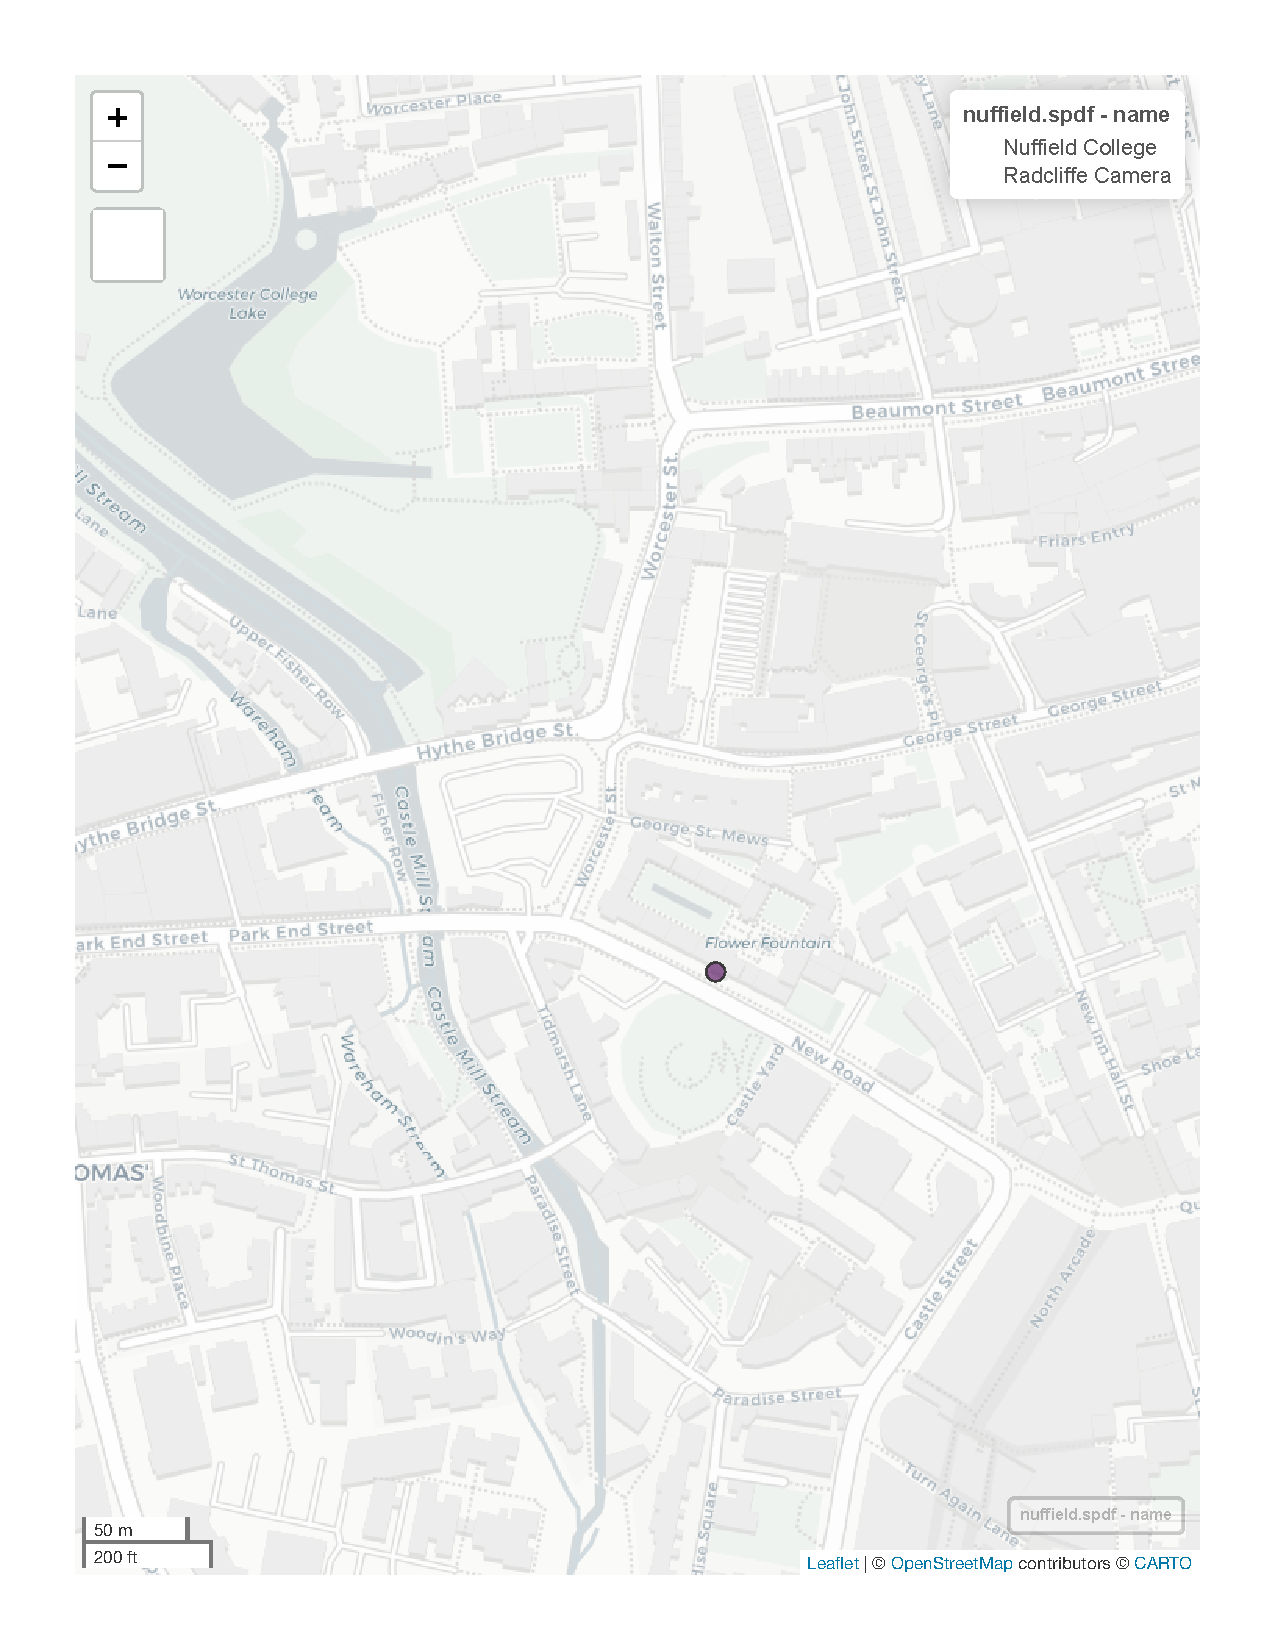
\includegraphics{01_refresher_files/figure-pdf/unnamed-chunk-4-1.pdf}

}

\end{figure}

\hypertarget{projected-crs}{%
\subsection{Projected CRS}\label{projected-crs}}

However, different data providers use different CRS. For instance,
spatial data in the UK usually uses `OSGB 1936 / British National Grid'
(\href{https://epsg.io/27700}{EPSG:27700}). Here, coordinates are in
meters, and projected onto a planar 2D space.

There are a lot of different CRS projections, and different national
statistics offices provide data in different projections. Data providers
usually specify which reference system they use. This is important as
using the correct reference system and projection is crucial for
plotting and manipulating spatial data.

If you do not know the correct CRS, try starting with a standards CRS
like \href{https://epsg.io/4326}{EPSG:4326} if you have decimal degree
like coordinates. If it looks like projected coordinates, try searching
for the country or region in CRS libraries like \url{https://epsg.io/}.
However, you must check if the projected coordinates match their real
location, e.g.~using \texttt{mapview()}.

\hypertarget{why-different-projections}{%
\subsection{Why different
projections?}\label{why-different-projections}}

By now, (most) people agree that
\href{https://r-spatial.org/r/2020/06/17/s2.html}{the earth is not
flat}. So, to plot data on a 2D planar surface and to perform certain
operations on a planar world, we need to make some re-projections.
Depending on where we are, different re-projections of our data (globe
in this case) might work better than others.

\begin{Shaded}
\begin{Highlighting}[]
\NormalTok{world }\OtherTok{\textless{}{-}} \FunctionTok{ne\_countries}\NormalTok{(}\AttributeTok{scale =} \StringTok{"medium"}\NormalTok{, }\AttributeTok{returnclass =} \StringTok{"sf"}\NormalTok{)}
\FunctionTok{class}\NormalTok{(world)}
\end{Highlighting}
\end{Shaded}

\begin{verbatim}
[1] "sf"         "data.frame"
\end{verbatim}

\begin{Shaded}
\begin{Highlighting}[]
\FunctionTok{st\_crs}\NormalTok{(world)}
\end{Highlighting}
\end{Shaded}

\begin{verbatim}
Coordinate Reference System:
  User input: WGS 84 
  wkt:
GEOGCRS["WGS 84",
    DATUM["World Geodetic System 1984",
        ELLIPSOID["WGS 84",6378137,298.257223563,
            LENGTHUNIT["metre",1]]],
    PRIMEM["Greenwich",0,
        ANGLEUNIT["degree",0.0174532925199433]],
    CS[ellipsoidal,2],
        AXIS["latitude",north,
            ORDER[1],
            ANGLEUNIT["degree",0.0174532925199433]],
        AXIS["longitude",east,
            ORDER[2],
            ANGLEUNIT["degree",0.0174532925199433]],
    ID["EPSG",4326]]
\end{verbatim}

\begin{Shaded}
\begin{Highlighting}[]
\CommentTok{\# Extract a country and plot in current CRS (WGS84)}
\NormalTok{ger.spdf }\OtherTok{\textless{}{-}}\NormalTok{ world[world}\SpecialCharTok{$}\NormalTok{name }\SpecialCharTok{==} \StringTok{"Germany"}\NormalTok{, ]}
\FunctionTok{plot}\NormalTok{(}\FunctionTok{st\_geometry}\NormalTok{(ger.spdf))}
\end{Highlighting}
\end{Shaded}

\begin{figure}[H]

{\centering 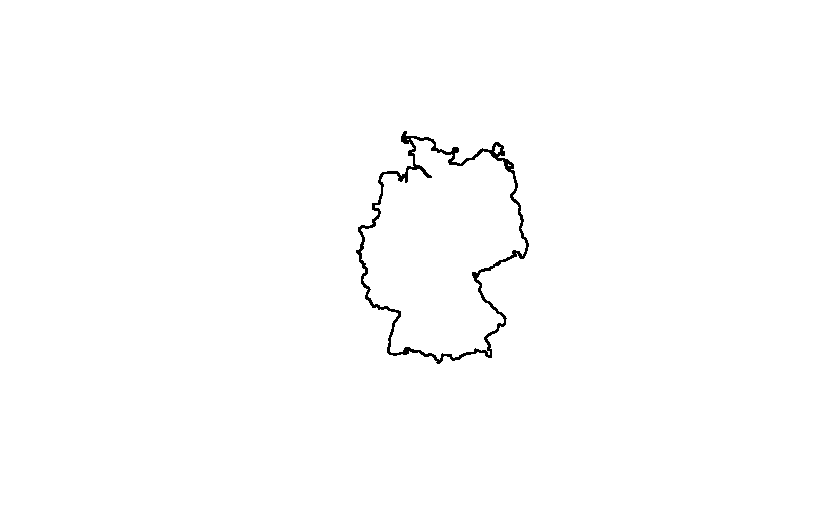
\includegraphics{01_refresher_files/figure-pdf/unnamed-chunk-5-1.pdf}

}

\end{figure}

\begin{Shaded}
\begin{Highlighting}[]
\CommentTok{\# Now, let\textquotesingle{}s transform Germany into a CRS optimized for Iceland}
\NormalTok{ger\_rep.spdf }\OtherTok{\textless{}{-}} \FunctionTok{st\_transform}\NormalTok{(ger.spdf, }\AttributeTok{crs =} \DecValTok{5325}\NormalTok{)}
\FunctionTok{plot}\NormalTok{(}\FunctionTok{st\_geometry}\NormalTok{(ger\_rep.spdf))}
\end{Highlighting}
\end{Shaded}

\begin{figure}[H]

{\centering 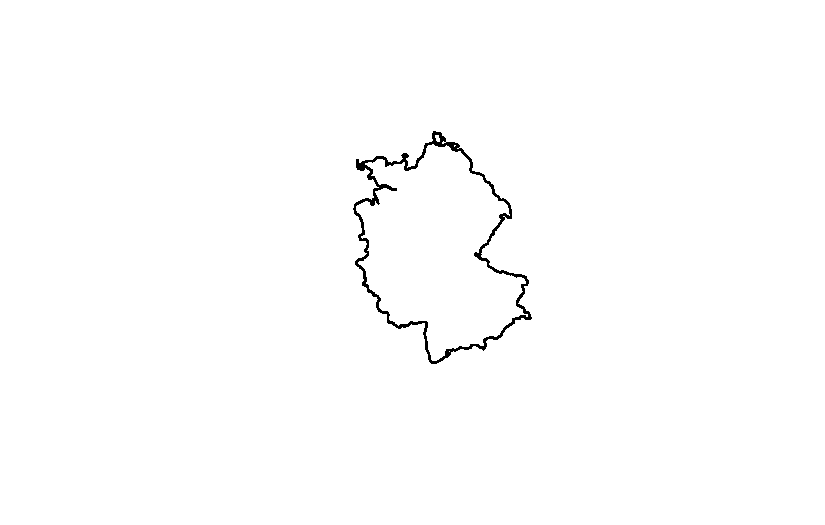
\includegraphics{01_refresher_files/figure-pdf/unnamed-chunk-5-2.pdf}

}

\end{figure}

Depending on the angle, a 2D projection of the earth looks different. It
is important to choose a suitable projection for the available spatial
data. For more information on CRS and re-projection, see e.g. Lovelace,
Nowosad, and Muenchow (2019) or
\href{https://stefanjuenger.github.io/}{Stefan Jünger} \&
\href{https://www.gesis.org/institut/mitarbeitendenverzeichnis/person/Anne-Kathrin.Stroppe}{Anne-Kathrin
Stroppe}'s
\href{https://github.com/StefanJuenger/gesis-workshop-geospatial-techniques-R-2023}{GESIS
workshop materials}.

\hypertarget{importing-some-real-world-data}{%
\section{Importing some real world
data}\label{importing-some-real-world-data}}

\texttt{sf} imports many of the most common spatial data files, like
geojson, gpkg, or shp.

\hypertarget{london-shapefile-polygon}{%
\subsection{London shapefile (polygon)}\label{london-shapefile-polygon}}

Let's get some administrative boundaries for London from the
\href{https://data.london.gov.uk/dataset/statistical-gis-boundary-files-london}{London
Datastore}. We use the \texttt{sf} package and its funtion
\texttt{st\_read()} to import the data.

\begin{Shaded}
\begin{Highlighting}[]
\CommentTok{\# Create subdir (all data withh be stored in "\_data")}
\NormalTok{dn }\OtherTok{\textless{}{-}} \StringTok{"\_data"}
\FunctionTok{ifelse}\NormalTok{(}\FunctionTok{dir.exists}\NormalTok{(dn), }\StringTok{"Exists"}\NormalTok{, }\FunctionTok{dir.create}\NormalTok{(dn))}
\end{Highlighting}
\end{Shaded}

\begin{verbatim}
[1] "Exists"
\end{verbatim}

\begin{Shaded}
\begin{Highlighting}[]
\CommentTok{\# Download zip file and unzip}
\NormalTok{tmpf }\OtherTok{\textless{}{-}} \FunctionTok{tempfile}\NormalTok{()}
\NormalTok{boundary.link }\OtherTok{\textless{}{-}} \StringTok{"https://data.london.gov.uk/download/statistical{-}gis{-}boundary{-}files{-}london/9ba8c833{-}6370{-}4b11{-}abdc{-}314aa020d5e0/statistical{-}gis{-}boundaries{-}london.zip"}
\FunctionTok{download.file}\NormalTok{(boundary.link, tmpf)}
\FunctionTok{unzip}\NormalTok{(}\AttributeTok{zipfile =}\NormalTok{ tmpf, }\AttributeTok{exdir =} \FunctionTok{paste0}\NormalTok{(dn))}
\FunctionTok{unlink}\NormalTok{(tmpf)}

\CommentTok{\# This is a shapefile}
\CommentTok{\# We only need the MSOA layer for now}
\NormalTok{msoa.spdf }\OtherTok{\textless{}{-}} \FunctionTok{st\_read}\NormalTok{(}\AttributeTok{dsn =} \FunctionTok{paste0}\NormalTok{(dn, }\StringTok{"/statistical{-}gis{-}boundaries{-}london/ESRI"}\NormalTok{),}
                     \AttributeTok{layer =} \StringTok{"MSOA\_2011\_London\_gen\_MHW"} \CommentTok{\# Note: no file ending}
\NormalTok{                     )}
\end{Highlighting}
\end{Shaded}

\begin{verbatim}
Reading layer `MSOA_2011_London_gen_MHW' from data source 
  `C:\work\Lehre\Geodata_Spatial_Regression\_data\statistical-gis-boundaries-london\ESRI' 
  using driver `ESRI Shapefile'
Simple feature collection with 983 features and 12 fields
Geometry type: MULTIPOLYGON
Dimension:     XY
Bounding box:  xmin: 503574.2 ymin: 155850.8 xmax: 561956.7 ymax: 200933.6
Projected CRS: OSGB36 / British National Grid
\end{verbatim}

The object \texttt{msoa.spdf} is our spatial data.frame. It looks
essentially like a conventional data.frame, but has some additional
attributes and geo-graphical information stored with it. Most
importantly, notice the column \texttt{geometry}, which contains a list
of polygons. In most cases, we have one polygon for each line /
observation.

\begin{Shaded}
\begin{Highlighting}[]
\FunctionTok{head}\NormalTok{(msoa.spdf)}
\end{Highlighting}
\end{Shaded}

\begin{verbatim}
Simple feature collection with 6 features and 12 fields
Geometry type: MULTIPOLYGON
Dimension:     XY
Bounding box:  xmin: 530966.7 ymin: 180510.7 xmax: 551943.8 ymax: 191139
Projected CRS: OSGB36 / British National Grid
   MSOA11CD                 MSOA11NM   LAD11CD              LAD11NM   RGN11CD
1 E02000001       City of London 001 E09000001       City of London E12000007
2 E02000002 Barking and Dagenham 001 E09000002 Barking and Dagenham E12000007
3 E02000003 Barking and Dagenham 002 E09000002 Barking and Dagenham E12000007
4 E02000004 Barking and Dagenham 003 E09000002 Barking and Dagenham E12000007
5 E02000005 Barking and Dagenham 004 E09000002 Barking and Dagenham E12000007
6 E02000007 Barking and Dagenham 006 E09000002 Barking and Dagenham E12000007
  RGN11NM USUALRES HHOLDRES COMESTRES POPDEN HHOLDS AVHHOLDSZ
1  London     7375     7187       188   25.5   4385       1.6
2  London     6775     6724        51   31.3   2713       2.5
3  London    10045    10033        12   46.9   3834       2.6
4  London     6182     5937       245   24.8   2318       2.6
5  London     8562     8562         0   72.1   3183       2.7
6  London     8791     8672       119   50.6   3441       2.5
                        geometry
1 MULTIPOLYGON (((531667.6 18...
2 MULTIPOLYGON (((548881.6 19...
3 MULTIPOLYGON (((549102.4 18...
4 MULTIPOLYGON (((551550 1873...
5 MULTIPOLYGON (((549099.6 18...
6 MULTIPOLYGON (((549819.9 18...
\end{verbatim}

Shapefiles are still among the most common formats to store and transmit
spatial data, despite them being inefficient (file size and file
number).

However, \texttt{sf} reads everything spatial, such as
\texttt{geo.json}, which usually is more efficient, but less common (but
we're getting there).

\begin{Shaded}
\begin{Highlighting}[]
\CommentTok{\# Download file}
\NormalTok{ulez.link }\OtherTok{\textless{}{-}} \StringTok{"https://data.london.gov.uk/download/ultra\_low\_emissions\_zone/936d71d8{-}c5fc{-}40ad{-}a392{-}6bec86413b48/CentralUltraLowEmissionZone.geojson"}
\FunctionTok{download.file}\NormalTok{(ulez.link, }\FunctionTok{paste0}\NormalTok{(dn, }\StringTok{"/ulez.json"}\NormalTok{))}

\CommentTok{\# Read geo.json}
\FunctionTok{st\_layers}\NormalTok{(}\FunctionTok{paste0}\NormalTok{(dn, }\StringTok{"/ulez.json"}\NormalTok{))}
\end{Highlighting}
\end{Shaded}

\begin{verbatim}
Driver: GeoJSON 
Available layers:
                   layer_name geometry_type features fields
1 CentralUltraLowEmissionZone Multi Polygon        1      4
                        crs_name
1 OSGB36 / British National Grid
\end{verbatim}

\begin{Shaded}
\begin{Highlighting}[]
\NormalTok{ulez.spdf }\OtherTok{\textless{}{-}} \FunctionTok{st\_read}\NormalTok{(}\AttributeTok{dsn =} \FunctionTok{paste0}\NormalTok{(dn, }\StringTok{"/ulez.json"}\NormalTok{)) }\CommentTok{\# here dsn is simply the file}
\end{Highlighting}
\end{Shaded}

\begin{verbatim}
Reading layer `CentralUltraLowEmissionZone' from data source 
  `C:\work\Lehre\Geodata_Spatial_Regression\_data\ulez.json' 
  using driver `GeoJSON'
Simple feature collection with 1 feature and 4 fields
Geometry type: MULTIPOLYGON
Dimension:     XY
Bounding box:  xmin: 527271.5 ymin: 178041.5 xmax: 533866.3 ymax: 183133.4
Projected CRS: OSGB36 / British National Grid
\end{verbatim}

\begin{Shaded}
\begin{Highlighting}[]
\FunctionTok{head}\NormalTok{(ulez.spdf)}
\end{Highlighting}
\end{Shaded}

\begin{verbatim}
Simple feature collection with 1 feature and 4 fields
Geometry type: MULTIPOLYGON
Dimension:     XY
Bounding box:  xmin: 527271.5 ymin: 178041.5 xmax: 533866.3 ymax: 183133.4
Projected CRS: OSGB36 / British National Grid
  fid OBJECTID BOUNDARY Shape_Area                       geometry
1   1        1 CSS Area   21.37557 MULTIPOLYGON (((531562.7 18...
\end{verbatim}

Again, this looks like a conventional \texttt{data.frame} but has the
additional column \texttt{geometry} containing the coordinates of each
observation. \texttt{st\_geometry()} returns only the geographic object
and \texttt{st\_drop\_geometry()} only the \texttt{data.frame} without
the coordinates. We can plot the object using \texttt{mapview()}.

\begin{Shaded}
\begin{Highlighting}[]
\FunctionTok{mapview}\NormalTok{(msoa.spdf[, }\StringTok{"POPDEN"}\NormalTok{])}
\end{Highlighting}
\end{Shaded}

\begin{figure}[H]

{\centering 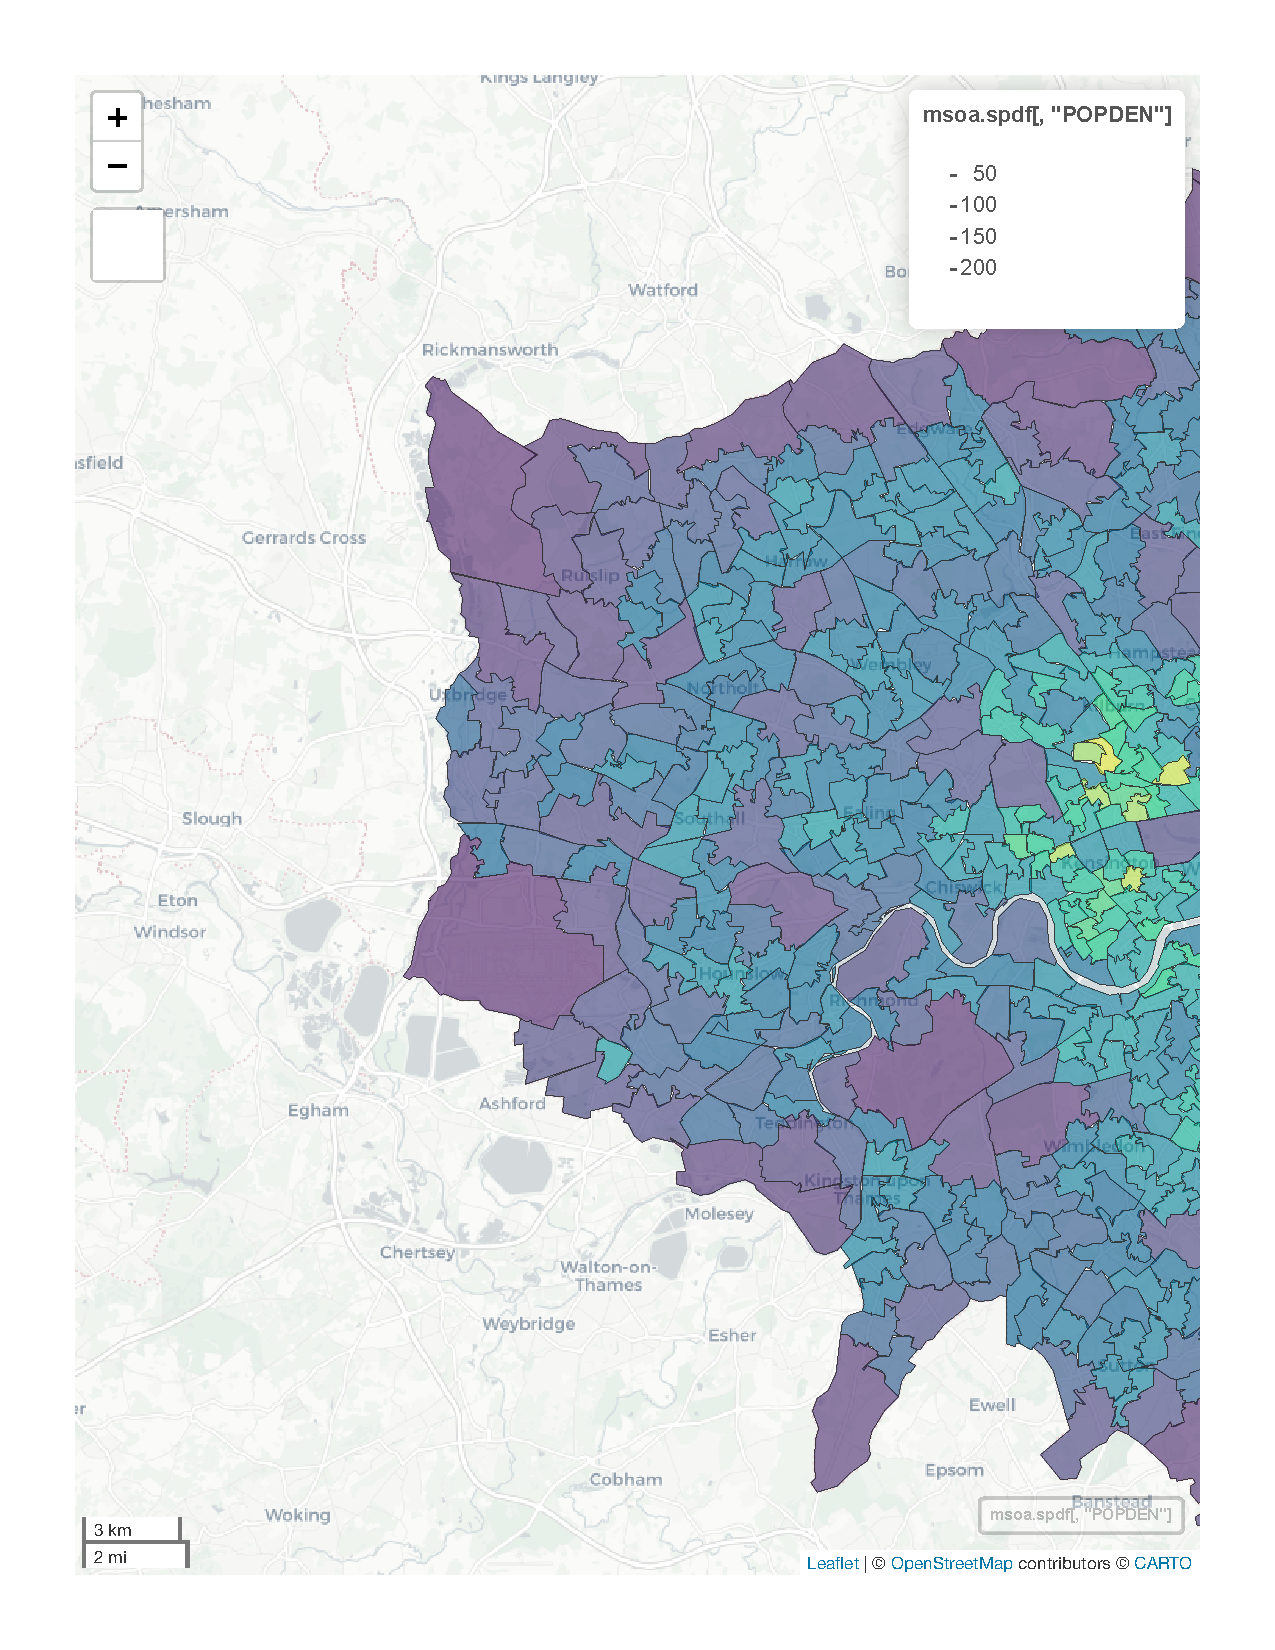
\includegraphics{01_refresher_files/figure-pdf/unnamed-chunk-9-1.pdf}

}

\end{figure}

\hypertarget{census-api-admin-units}{%
\subsection{Census API (admin units)}\label{census-api-admin-units}}

Now that we have some boundaries and shapes of spatial units in London,
we can start looking for different data sources to populate the
geometries.

A good source for demographic data is for instance the 2011 census.
Below we use the nomis API to retrieve population data for London, See
the
\href{https://cran.r-project.org/web/packages/nomisr/vignettes/introduction.html}{Vignette}
for more information (Guest users are limited to 25,000 rows per query).
Below is a wrapper to avoid some errors with sex and urban-rural
cross-tabulation in some of the data.

\begin{Shaded}
\begin{Highlighting}[]
\DocumentationTok{\#\#\# For larger request, register and set key}
\CommentTok{\# Sys.setenv(NOMIS\_API\_KEY = "XXX")}
\CommentTok{\# nomis\_api\_key(check\_env = TRUE)}

\NormalTok{x }\OtherTok{\textless{}{-}} \FunctionTok{nomis\_data\_info}\NormalTok{()}

\CommentTok{\# Get London ids}
\NormalTok{london\_ids }\OtherTok{\textless{}{-}}\NormalTok{ msoa.spdf}\SpecialCharTok{$}\NormalTok{MSOA11CD}

\DocumentationTok{\#\#\# Get key statistics ids}
\CommentTok{\# select requires tables (https://www.nomisweb.co.uk/sources/census\_2011\_ks)}
\CommentTok{\# Let\textquotesingle{}s get KS201EW (ethnic group), KS205EW (passport held), and KS402EW (housing tenure)}

\CommentTok{\# Get internal ids}
\NormalTok{stats }\OtherTok{\textless{}{-}} \FunctionTok{c}\NormalTok{(}\StringTok{"KS201EW"}\NormalTok{, }\StringTok{"KS402EW"}\NormalTok{, }\StringTok{"KS205EW"}\NormalTok{)}
\NormalTok{oo }\OtherTok{\textless{}{-}} \FunctionTok{which}\NormalTok{(}\FunctionTok{grepl}\NormalTok{(}\FunctionTok{paste}\NormalTok{(stats, }\AttributeTok{collapse =} \StringTok{"|"}\NormalTok{), x}\SpecialCharTok{$}\NormalTok{name.value))}
\NormalTok{ksids }\OtherTok{\textless{}{-}}\NormalTok{ x}\SpecialCharTok{$}\NormalTok{id[oo]}
\NormalTok{ksids }\CommentTok{\# This are the internal ids}
\end{Highlighting}
\end{Shaded}

\begin{verbatim}
[1] "NM_608_1" "NM_612_1" "NM_619_1"
\end{verbatim}

\begin{Shaded}
\begin{Highlighting}[]
\DocumentationTok{\#\#\# look at meta information}
\NormalTok{q }\OtherTok{\textless{}{-}} \FunctionTok{nomis\_overview}\NormalTok{(ksids[}\DecValTok{1}\NormalTok{])}
\FunctionTok{head}\NormalTok{(q)}
\end{Highlighting}
\end{Shaded}

\begin{verbatim}
# A tibble: 6 x 2
  name           value           
  <chr>          <list>          
1 analyses       <named list [1]>
2 analysisname   <chr [1]>       
3 analysisnumber <int [1]>       
4 contact        <named list [4]>
5 contenttypes   <named list [1]>
6 coverage       <chr [1]>       
\end{verbatim}

\begin{Shaded}
\begin{Highlighting}[]
\NormalTok{a }\OtherTok{\textless{}{-}} \FunctionTok{nomis\_get\_metadata}\NormalTok{(}\AttributeTok{id =}\NormalTok{ ksids[}\DecValTok{1}\NormalTok{], }\AttributeTok{concept =} \StringTok{"GEOGRAPHY"}\NormalTok{, }\AttributeTok{type =} \StringTok{"type"}\NormalTok{)}
\NormalTok{a }\CommentTok{\# TYPE297 is MSOA level}
\end{Highlighting}
\end{Shaded}

\begin{verbatim}
# A tibble: 24 x 3
   id      label.en                                           description.en    
   <chr>   <chr>                                              <chr>             
 1 TYPE265 NHS area teams                                     NHS area teams    
 2 TYPE266 clinical commissioning groups                      clinical commissi~
 3 TYPE267 built-up areas including subdivisions              built-up areas in~
 4 TYPE269 built-up areas                                     built-up areas    
 5 TYPE273 national assembly for wales electoral regions 2010 national assembly~
 6 TYPE274 postcode areas                                     postcode areas    
 7 TYPE275 postcode districts                                 postcode districts
 8 TYPE276 postcode sectors                                   postcode sectors  
 9 TYPE277 national assembly for wales constituencies 2010    national assembly~
10 TYPE279 parishes 2011                                      parishes 2011     
# i 14 more rows
\end{verbatim}

\begin{Shaded}
\begin{Highlighting}[]
\NormalTok{b }\OtherTok{\textless{}{-}} \FunctionTok{nomis\_get\_metadata}\NormalTok{(}\AttributeTok{id =}\NormalTok{ ksids[}\DecValTok{1}\NormalTok{], }\AttributeTok{concept =} \StringTok{"MEASURES"}\NormalTok{, }\AttributeTok{type =} \StringTok{"TYPE297"}\NormalTok{)}
\NormalTok{b }\CommentTok{\# 20100 is the measure of absolute numbers}
\end{Highlighting}
\end{Shaded}

\begin{verbatim}
# A tibble: 2 x 3
  id    label.en description.en
  <chr> <chr>    <chr>         
1 20100 value    value         
2 20301 percent  percent       
\end{verbatim}

\begin{Shaded}
\begin{Highlighting}[]
\DocumentationTok{\#\#\# Query data in loop over the required statistics}
\ControlFlowTok{for}\NormalTok{(i }\ControlFlowTok{in}\NormalTok{ ksids)\{}

  \CommentTok{\# Determin if data is divided by sex or urban{-}rural}
\NormalTok{  nd }\OtherTok{\textless{}{-}} \FunctionTok{nomis\_get\_metadata}\NormalTok{(}\AttributeTok{id =}\NormalTok{ i)}
  \ControlFlowTok{if}\NormalTok{(}\StringTok{"RURAL\_URBAN"} \SpecialCharTok{\%in\%}\NormalTok{ nd}\SpecialCharTok{$}\NormalTok{conceptref)\{}
\NormalTok{    UR }\OtherTok{\textless{}{-}} \ConstantTok{TRUE}
\NormalTok{  \}}\ControlFlowTok{else}\NormalTok{\{}
\NormalTok{    UR }\OtherTok{\textless{}{-}} \ConstantTok{FALSE}
\NormalTok{  \}}
  \ControlFlowTok{if}\NormalTok{(}\StringTok{"C\_SEX"} \SpecialCharTok{\%in\%}\NormalTok{ nd}\SpecialCharTok{$}\NormalTok{conceptref)\{}
\NormalTok{    SEX }\OtherTok{\textless{}{-}} \ConstantTok{TRUE}
\NormalTok{  \}}\ControlFlowTok{else}\NormalTok{\{}
\NormalTok{    SEX }\OtherTok{\textless{}{-}} \ConstantTok{FALSE}
\NormalTok{  \}}

  \CommentTok{\# make data request}
  \ControlFlowTok{if}\NormalTok{(UR }\SpecialCharTok{==} \ConstantTok{TRUE}\NormalTok{)\{}
    \ControlFlowTok{if}\NormalTok{(SEX }\SpecialCharTok{==} \ConstantTok{TRUE}\NormalTok{)\{}
\NormalTok{      tmp\_en }\OtherTok{\textless{}{-}} \FunctionTok{nomis\_get\_data}\NormalTok{(}\AttributeTok{id =}\NormalTok{ i, }\AttributeTok{time =} \StringTok{"2011"}\NormalTok{,}
                               \AttributeTok{geography =}\NormalTok{ london\_ids, }\CommentTok{\# replace with "TYPE297" for all MSOAs}
                               \AttributeTok{measures =} \DecValTok{20100}\NormalTok{, }\AttributeTok{RURAL\_URBAN =} \DecValTok{0}\NormalTok{, }\AttributeTok{C\_SEX =} \DecValTok{0}\NormalTok{)}
\NormalTok{    \}}\ControlFlowTok{else}\NormalTok{\{}
\NormalTok{      tmp\_en }\OtherTok{\textless{}{-}} \FunctionTok{nomis\_get\_data}\NormalTok{(}\AttributeTok{id =}\NormalTok{ i, }\AttributeTok{time =} \StringTok{"2011"}\NormalTok{,}
                               \AttributeTok{geography =}\NormalTok{ london\_ids, }\CommentTok{\# replace with "TYPE297" for all MSOAs}
                               \AttributeTok{measures =} \DecValTok{20100}\NormalTok{, }\AttributeTok{RURAL\_URBAN =} \DecValTok{0}\NormalTok{)}
\NormalTok{    \}}
\NormalTok{  \}}\ControlFlowTok{else}\NormalTok{\{}
    \ControlFlowTok{if}\NormalTok{(SEX }\SpecialCharTok{==} \ConstantTok{TRUE}\NormalTok{)\{}
\NormalTok{      tmp\_en }\OtherTok{\textless{}{-}} \FunctionTok{nomis\_get\_data}\NormalTok{(}\AttributeTok{id =}\NormalTok{ i, }\AttributeTok{time =} \StringTok{"2011"}\NormalTok{,}
                               \AttributeTok{geography =}\NormalTok{ london\_ids, }\CommentTok{\# replace with "TYPE297" for all MSOAs}
                               \AttributeTok{measures =} \DecValTok{20100}\NormalTok{, }\AttributeTok{C\_SEX =} \DecValTok{0}\NormalTok{)}
\NormalTok{    \}}\ControlFlowTok{else}\NormalTok{\{}
\NormalTok{      tmp\_en }\OtherTok{\textless{}{-}} \FunctionTok{nomis\_get\_data}\NormalTok{(}\AttributeTok{id =}\NormalTok{ i, }\AttributeTok{time =} \StringTok{"2011"}\NormalTok{,}
                               \AttributeTok{geography =}\NormalTok{ london\_ids, }\CommentTok{\# replace with "TYPE297" for all MSOAs}
                               \AttributeTok{measures =} \DecValTok{20100}\NormalTok{)}
\NormalTok{    \}}

\NormalTok{  \}}

  \CommentTok{\# Append (in case of different regions)}
\NormalTok{  ks\_tmp }\OtherTok{\textless{}{-}}\NormalTok{ tmp\_en}

  \CommentTok{\# Make lower case names}
  \FunctionTok{names}\NormalTok{(ks\_tmp) }\OtherTok{\textless{}{-}} \FunctionTok{tolower}\NormalTok{(}\FunctionTok{names}\NormalTok{(ks\_tmp))}
  \FunctionTok{names}\NormalTok{(ks\_tmp)[}\FunctionTok{names}\NormalTok{(ks\_tmp) }\SpecialCharTok{==} \StringTok{"geography\_code"}\NormalTok{] }\OtherTok{\textless{}{-}} \StringTok{"msoa11"}
  \FunctionTok{names}\NormalTok{(ks\_tmp)[}\FunctionTok{names}\NormalTok{(ks\_tmp) }\SpecialCharTok{==} \StringTok{"geography\_name"}\NormalTok{] }\OtherTok{\textless{}{-}} \StringTok{"name"}

  \CommentTok{\# replace weird cell codes}
\NormalTok{  onlynum }\OtherTok{\textless{}{-}} \FunctionTok{which}\NormalTok{(}\FunctionTok{grepl}\NormalTok{(}\StringTok{"\^{}[[:digit:]]+$"}\NormalTok{, ks\_tmp}\SpecialCharTok{$}\NormalTok{cell\_code))}
  \ControlFlowTok{if}\NormalTok{(}\FunctionTok{length}\NormalTok{(onlynum) }\SpecialCharTok{!=} \DecValTok{0}\NormalTok{)\{}
\NormalTok{    code }\OtherTok{\textless{}{-}} \FunctionTok{substr}\NormalTok{(ks\_tmp}\SpecialCharTok{$}\NormalTok{cell\_code[}\SpecialCharTok{{-}}\NormalTok{onlynum][}\DecValTok{1}\NormalTok{], }\DecValTok{1}\NormalTok{, }\DecValTok{7}\NormalTok{)}
    \ControlFlowTok{if}\NormalTok{(}\FunctionTok{is.na}\NormalTok{(code))\{}
\NormalTok{      code }\OtherTok{\textless{}{-}}\NormalTok{ i}
\NormalTok{    \}}
\NormalTok{    ks\_tmp}\SpecialCharTok{$}\NormalTok{cell\_code[onlynum] }\OtherTok{\textless{}{-}} \FunctionTok{paste0}\NormalTok{(code, }\StringTok{"\_"}\NormalTok{, ks\_tmp}\SpecialCharTok{$}\NormalTok{cell\_code[onlynum])}
\NormalTok{  \}}

  \CommentTok{\# save codebook}
\NormalTok{  ks\_cb }\OtherTok{\textless{}{-}} \FunctionTok{unique}\NormalTok{(ks\_tmp[, }\FunctionTok{c}\NormalTok{(}\StringTok{"date"}\NormalTok{, }\StringTok{"cell\_type"}\NormalTok{, }\StringTok{"cell"}\NormalTok{, }\StringTok{"cell\_code"}\NormalTok{, }\StringTok{"cell\_name"}\NormalTok{)])}

  \DocumentationTok{\#\#\# Reshape}
\NormalTok{  ks\_res }\OtherTok{\textless{}{-}}\NormalTok{ tidyr}\SpecialCharTok{::}\FunctionTok{pivot\_wider}\NormalTok{(ks\_tmp, }\AttributeTok{id\_cols =} \FunctionTok{c}\NormalTok{(}\StringTok{"msoa11"}\NormalTok{, }\StringTok{"name"}\NormalTok{),}
                               \AttributeTok{names\_from =} \StringTok{"cell\_code"}\NormalTok{,}
                               \AttributeTok{values\_from =} \StringTok{"obs\_value"}\NormalTok{)}

  \DocumentationTok{\#\#\# Merge}
  \ControlFlowTok{if}\NormalTok{(i }\SpecialCharTok{==}\NormalTok{ ksids[}\DecValTok{1}\NormalTok{])\{}
\NormalTok{    census\_keystat.df }\OtherTok{\textless{}{-}}\NormalTok{ ks\_res}
\NormalTok{    census\_keystat\_cb.df }\OtherTok{\textless{}{-}}\NormalTok{ ks\_cb}
\NormalTok{  \}}\ControlFlowTok{else}\NormalTok{\{}
\NormalTok{    census\_keystat.df }\OtherTok{\textless{}{-}} \FunctionTok{merge}\NormalTok{(census\_keystat.df, ks\_res, }\AttributeTok{by =} \FunctionTok{c}\NormalTok{(}\StringTok{"msoa11"}\NormalTok{, }\StringTok{"name"}\NormalTok{), }\AttributeTok{all =} \ConstantTok{TRUE}\NormalTok{)}
\NormalTok{    census\_keystat\_cb.df }\OtherTok{\textless{}{-}} \FunctionTok{rbind}\NormalTok{(census\_keystat\_cb.df, ks\_cb)}
\NormalTok{  \}}

\NormalTok{\}}


\CommentTok{\# Descriptions are saved in the codebook}
\FunctionTok{head}\NormalTok{(census\_keystat\_cb.df)}
\end{Highlighting}
\end{Shaded}

\begin{verbatim}
# A tibble: 6 x 5
   date cell_type     cell cell_code   cell_name                                
  <dbl> <chr>        <dbl> <chr>       <chr>                                    
1  2011 Ethnic Group     0 KS201EW0001 All usual residents                      
2  2011 Ethnic Group   100 KS201EW_100 White                                    
3  2011 Ethnic Group     1 KS201EW0002 White: English/Welsh/Scottish/Northern I~
4  2011 Ethnic Group     2 KS201EW0003 White: Irish                             
5  2011 Ethnic Group     3 KS201EW0004 White: Gypsy or Irish Traveller          
6  2011 Ethnic Group     4 KS201EW0005 White: Other White                       
\end{verbatim}

\begin{Shaded}
\begin{Highlighting}[]
\FunctionTok{save}\NormalTok{(census\_keystat\_cb.df, }\AttributeTok{file =} \StringTok{"\_data/Census\_codebook.RData"}\NormalTok{)}
\end{Highlighting}
\end{Shaded}

Now, we have one file containing the geometries of MSOAs and one file
with the census information on ethnic groups. Obviously, we can easily
merge them together using the MSOA identifiers.

\begin{Shaded}
\begin{Highlighting}[]
\NormalTok{msoa.spdf }\OtherTok{\textless{}{-}} \FunctionTok{merge}\NormalTok{(msoa.spdf, census\_keystat.df,}
                   \AttributeTok{by.x =} \StringTok{"MSOA11CD"}\NormalTok{, }\AttributeTok{by.y =} \StringTok{"msoa11"}\NormalTok{, }\AttributeTok{all.x =} \ConstantTok{TRUE}\NormalTok{)}
\end{Highlighting}
\end{Shaded}

And we can, for instance, plot the spatial distribution of ethnic
groups.

\begin{Shaded}
\begin{Highlighting}[]
\NormalTok{msoa.spdf}\SpecialCharTok{$}\NormalTok{per\_white }\OtherTok{\textless{}{-}}\NormalTok{ msoa.spdf}\SpecialCharTok{$}\NormalTok{KS201EW\_100 }\SpecialCharTok{/}\NormalTok{ msoa.spdf}\SpecialCharTok{$}\NormalTok{KS201EW0001 }\SpecialCharTok{*} \DecValTok{100}
\NormalTok{msoa.spdf}\SpecialCharTok{$}\NormalTok{per\_mixed }\OtherTok{\textless{}{-}}\NormalTok{ msoa.spdf}\SpecialCharTok{$}\NormalTok{KS201EW\_200 }\SpecialCharTok{/}\NormalTok{ msoa.spdf}\SpecialCharTok{$}\NormalTok{KS201EW0001 }\SpecialCharTok{*} \DecValTok{100}
\NormalTok{msoa.spdf}\SpecialCharTok{$}\NormalTok{per\_asian }\OtherTok{\textless{}{-}}\NormalTok{ msoa.spdf}\SpecialCharTok{$}\NormalTok{KS201EW\_300 }\SpecialCharTok{/}\NormalTok{ msoa.spdf}\SpecialCharTok{$}\NormalTok{KS201EW0001 }\SpecialCharTok{*} \DecValTok{100}
\NormalTok{msoa.spdf}\SpecialCharTok{$}\NormalTok{per\_black }\OtherTok{\textless{}{-}}\NormalTok{ msoa.spdf}\SpecialCharTok{$}\NormalTok{KS201EW\_400 }\SpecialCharTok{/}\NormalTok{ msoa.spdf}\SpecialCharTok{$}\NormalTok{KS201EW0001 }\SpecialCharTok{*} \DecValTok{100}
\NormalTok{msoa.spdf}\SpecialCharTok{$}\NormalTok{per\_other }\OtherTok{\textless{}{-}}\NormalTok{ msoa.spdf}\SpecialCharTok{$}\NormalTok{KS201EW\_500 }\SpecialCharTok{/}\NormalTok{ msoa.spdf}\SpecialCharTok{$}\NormalTok{KS201EW0001 }\SpecialCharTok{*} \DecValTok{100}

\FunctionTok{mapview}\NormalTok{(msoa.spdf[, }\StringTok{"per\_white"}\NormalTok{])}
\end{Highlighting}
\end{Shaded}

\begin{figure}[H]

{\centering 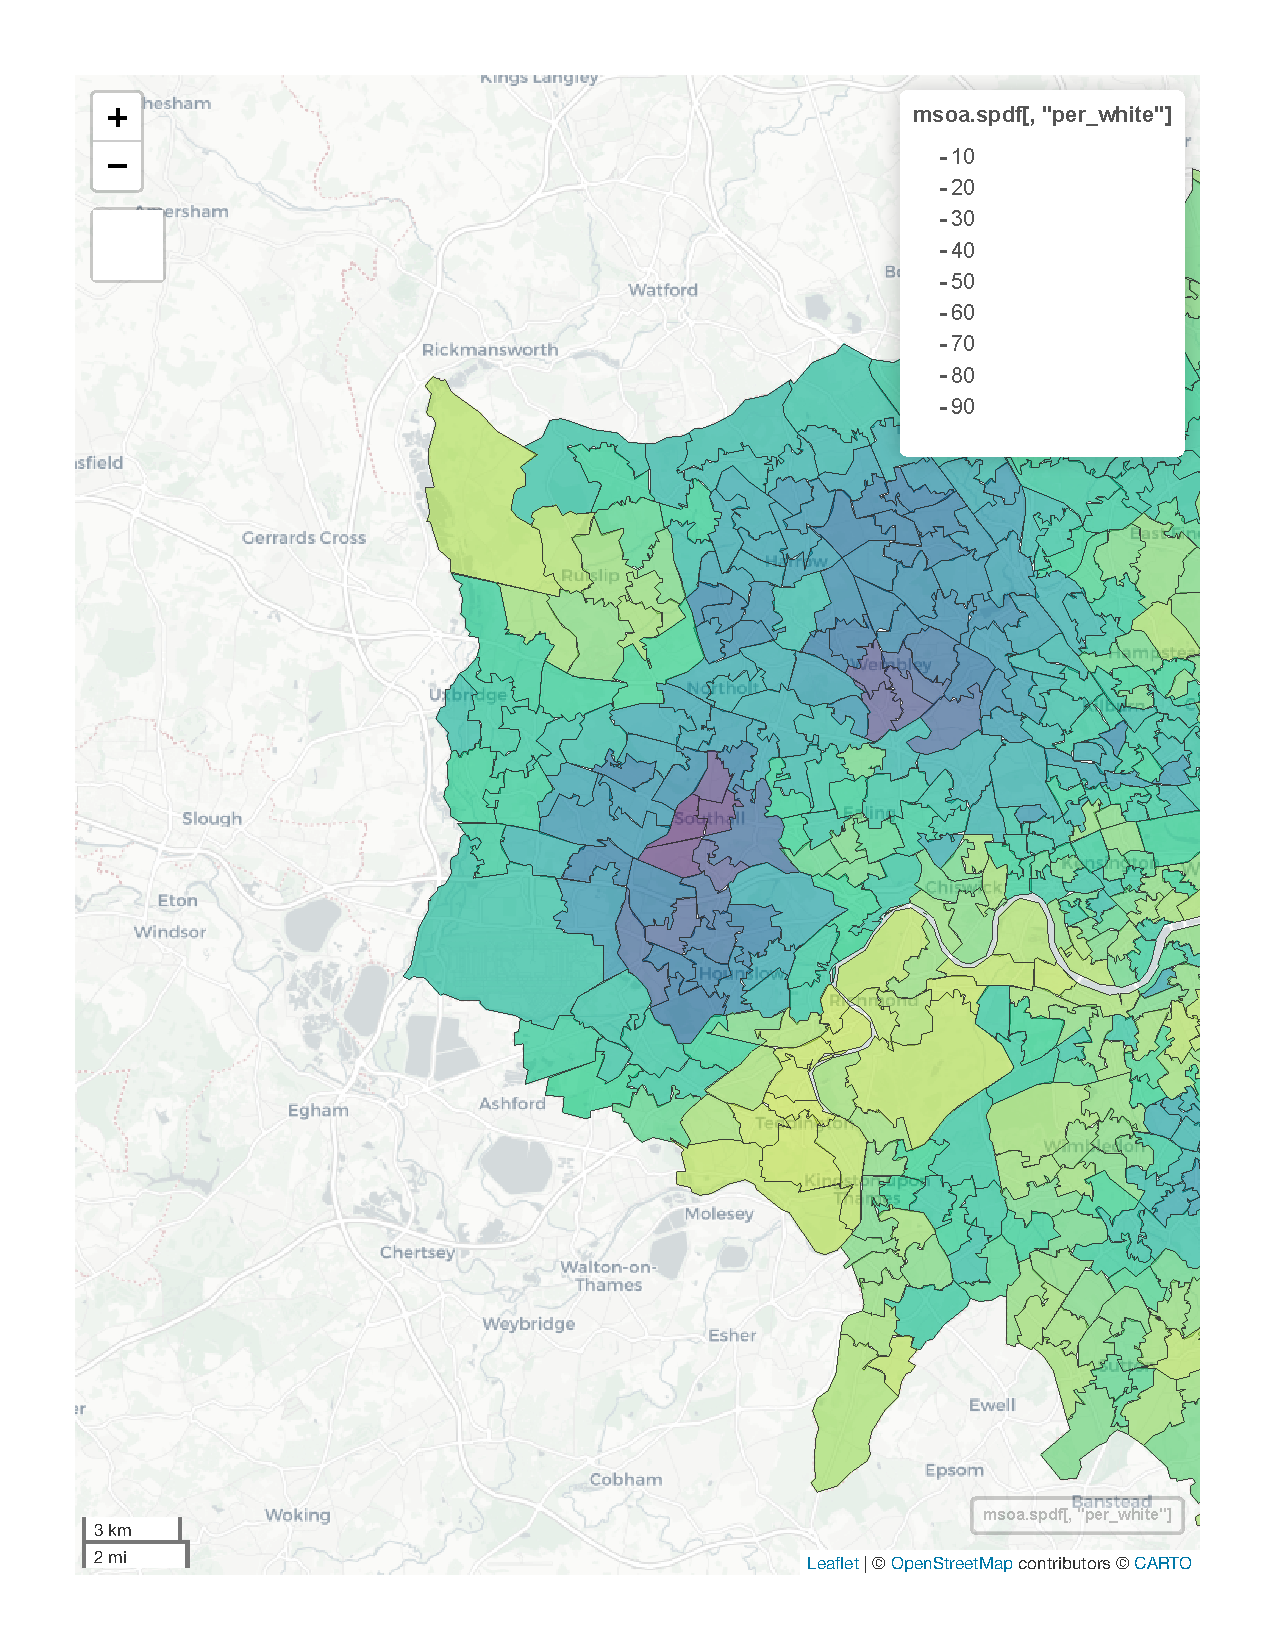
\includegraphics{01_refresher_files/figure-pdf/unnamed-chunk-12-1.pdf}

}

\end{figure}

If you're interested in more data sources, see for instance
\href{https://bookdown.org/paul/apis_for_social_scientists/}{APIs for
social scientists: A collaborative review} by Paul C. Bauer, Camille
Landesvatter, Lion Behrens. It's a collection of several APIs for social
sciences.

\hypertarget{gridded-data}{%
\subsection{Gridded data}\label{gridded-data}}

So far, we have queried data on administrative units. However, often
data comes on other spatial scales. For instance, we might be interested
in the amount of air pollution, which is provided on a regular grid
across the UK from
\href{https://uk-air.defra.gov.uk/data/pcm-data}{Defra}.

\begin{Shaded}
\begin{Highlighting}[]
\CommentTok{\# Download}
\NormalTok{pol.link }\OtherTok{\textless{}{-}} \StringTok{"https://uk{-}air.defra.gov.uk/datastore/pcm/mapno22011.csv"}
\FunctionTok{download.file}\NormalTok{(pol.link, }\FunctionTok{paste0}\NormalTok{(dn, }\StringTok{"/mapno22011.csv"}\NormalTok{))}
\NormalTok{pol.df }\OtherTok{\textless{}{-}} \FunctionTok{read.csv}\NormalTok{(}\FunctionTok{paste0}\NormalTok{(dn, }\StringTok{"/mapno22011.csv"}\NormalTok{), }\AttributeTok{skip =} \DecValTok{5}\NormalTok{, }\AttributeTok{header =}\NormalTok{ T, }\AttributeTok{sep =} \StringTok{","}\NormalTok{,}
                      \AttributeTok{stringsAsFactors =}\NormalTok{ F, }\AttributeTok{na.strings =} \StringTok{"MISSING"}\NormalTok{)}

\FunctionTok{head}\NormalTok{(pol.df)}
\end{Highlighting}
\end{Shaded}

\begin{verbatim}
  ukgridcode      x       y no22011
1      54291 460500 1221500      NA
2      54292 461500 1221500      NA
3      54294 463500 1221500      NA
4      54979 458500 1220500      NA
5      54980 459500 1220500      NA
6      54981 460500 1220500      NA
\end{verbatim}

The data comes as point data with x and y as coordinates. We have to
transform this into spatial data first. We first setup a spatial points
object with \texttt{st\_as\_sf}. Subsequently, we transform the point
coordinates into a regular grid. We use a buffer method
\texttt{st\_buffer} with ``diameter'', and only one segment per quadrant
(\texttt{nQuadSegs}). This gives us a 1x1km regular grid.

\begin{Shaded}
\begin{Highlighting}[]
\CommentTok{\# Build spatial object}
\NormalTok{pol.spdf }\OtherTok{\textless{}{-}} \FunctionTok{st\_as\_sf}\NormalTok{(pol.df, }\AttributeTok{coords =} \FunctionTok{c}\NormalTok{(}\StringTok{"x"}\NormalTok{, }\StringTok{"y"}\NormalTok{),}
                    \AttributeTok{crs =} \DecValTok{27700}\NormalTok{)}

\CommentTok{\# we transform the point coordinates into a regular grid with "diameter" 500m}
\NormalTok{pol.spdf }\OtherTok{\textless{}{-}} \FunctionTok{st\_buffer}\NormalTok{(pol.spdf, }\AttributeTok{dist =} \DecValTok{500}\NormalTok{, }\AttributeTok{nQuadSegs  =} \DecValTok{1}\NormalTok{,}
                      \AttributeTok{endCapStyle =} \StringTok{\textquotesingle{}SQUARE\textquotesingle{}}\NormalTok{)}

\CommentTok{\# Plot NO2}
\FunctionTok{plot}\NormalTok{(pol.spdf[, }\StringTok{"no22011"}\NormalTok{], }\AttributeTok{border =} \ConstantTok{NA}\NormalTok{)}
\end{Highlighting}
\end{Shaded}

\begin{figure}[H]

{\centering 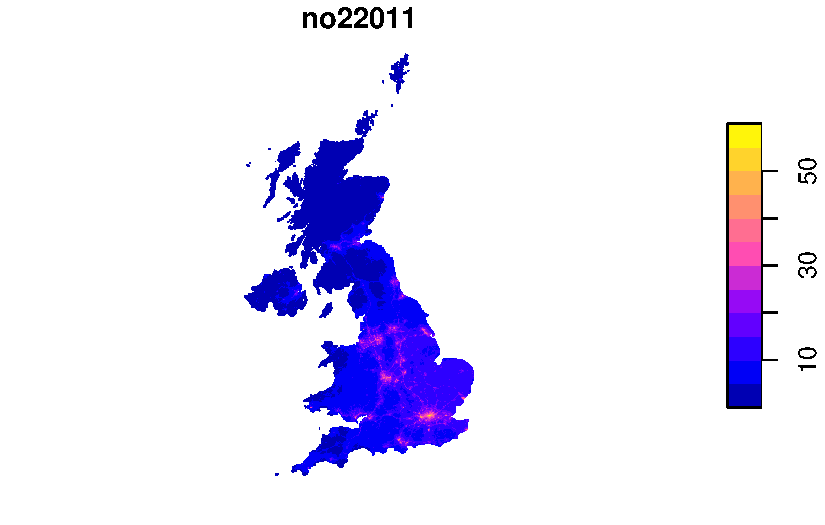
\includegraphics{01_refresher_files/figure-pdf/unnamed-chunk-14-1.pdf}

}

\end{figure}

\hypertarget{openstreetmap-points}{%
\subsection{OpenStreetMap (points)}\label{openstreetmap-points}}

Another interesting data source is the OpenStreetMap API, which provides
information about the geographical location of a serious of different
indicators. Robin Lovelace provides a nice introduction to the
\href{https://cran.r-project.org/web/packages/osmdata/vignettes/osmdata.html}{osmdata
API}. Available features can be found on
\href{https://wiki.openstreetmap.org/wiki/Map_features}{OSM wiki}.

First we create a bounding box of where we want to query data.
\texttt{st\_bbox()} can be used to get bounding boxes of an existing
spatial object (needs \texttt{CRS\ =\ 4326}). An alternative would be to
use
\texttt{opq(bbox\ =\ \textquotesingle{}greater\ london\ uk\textquotesingle{})}.

\begin{Shaded}
\begin{Highlighting}[]
\CommentTok{\# bounding box of where we want to query data}
\NormalTok{q }\OtherTok{\textless{}{-}} \FunctionTok{opq}\NormalTok{(}\AttributeTok{bbox =} \FunctionTok{st\_bbox}\NormalTok{(}\FunctionTok{st\_transform}\NormalTok{(msoa.spdf, }\DecValTok{4326}\NormalTok{)))}
\end{Highlighting}
\end{Shaded}

And we want to get data for all pubs and bars which are within this
bounding box.

\begin{Shaded}
\begin{Highlighting}[]
\CommentTok{\# First build the query of location of pubs in London}
\NormalTok{osmq }\OtherTok{\textless{}{-}} \FunctionTok{add\_osm\_feature}\NormalTok{(q, }\AttributeTok{key =} \StringTok{"amenity"}\NormalTok{, }\AttributeTok{value =} \StringTok{"pub"}\NormalTok{)}

\CommentTok{\# And then query the data}
\NormalTok{pubs.osm }\OtherTok{\textless{}{-}} \FunctionTok{osmdata\_sf}\NormalTok{(osmq)}
\end{Highlighting}
\end{Shaded}

Right now there are some results in polygons, some in points, and they
overlap. Often, data from OSM needs some manual cleaning. Sometimes the
same features are represented by different spatial objects (e.g.~points
+ polygons).

\begin{Shaded}
\begin{Highlighting}[]
\CommentTok{\# Make unique points / polygons}
\NormalTok{pubs.osm }\OtherTok{\textless{}{-}} \FunctionTok{unique\_osmdata}\NormalTok{(pubs.osm)}

\CommentTok{\# Get points and polygons (there are barley any pubs as polygons, so we ignore them)}
\NormalTok{pubs.points }\OtherTok{\textless{}{-}}\NormalTok{ pubs.osm}\SpecialCharTok{$}\NormalTok{osm\_points}
\NormalTok{pubs.polys }\OtherTok{\textless{}{-}}\NormalTok{ pubs.osm}\SpecialCharTok{$}\NormalTok{osm\_multipolygons}

\CommentTok{\# \# Drop OSM file}
\CommentTok{\# rm(pubs.osm); gc()}

\CommentTok{\# Reduce to point object only}
\NormalTok{pubs.spdf }\OtherTok{\textless{}{-}}\NormalTok{ pubs.points}

\CommentTok{\# Reduce to a few variables}
\NormalTok{pubs.spdf }\OtherTok{\textless{}{-}}\NormalTok{ pubs.spdf[, }\FunctionTok{c}\NormalTok{(}\StringTok{"osm\_id"}\NormalTok{, }\StringTok{"name"}\NormalTok{, }\StringTok{"addr:postcode"}\NormalTok{, }\StringTok{"diet:vegan"}\NormalTok{)]}
\end{Highlighting}
\end{Shaded}

Again, we can inspect the results with \texttt{mapview}.

\begin{Shaded}
\begin{Highlighting}[]
\FunctionTok{mapview}\NormalTok{(}\FunctionTok{st\_geometry}\NormalTok{(pubs.spdf))}
\end{Highlighting}
\end{Shaded}

\begin{figure}[H]

{\centering 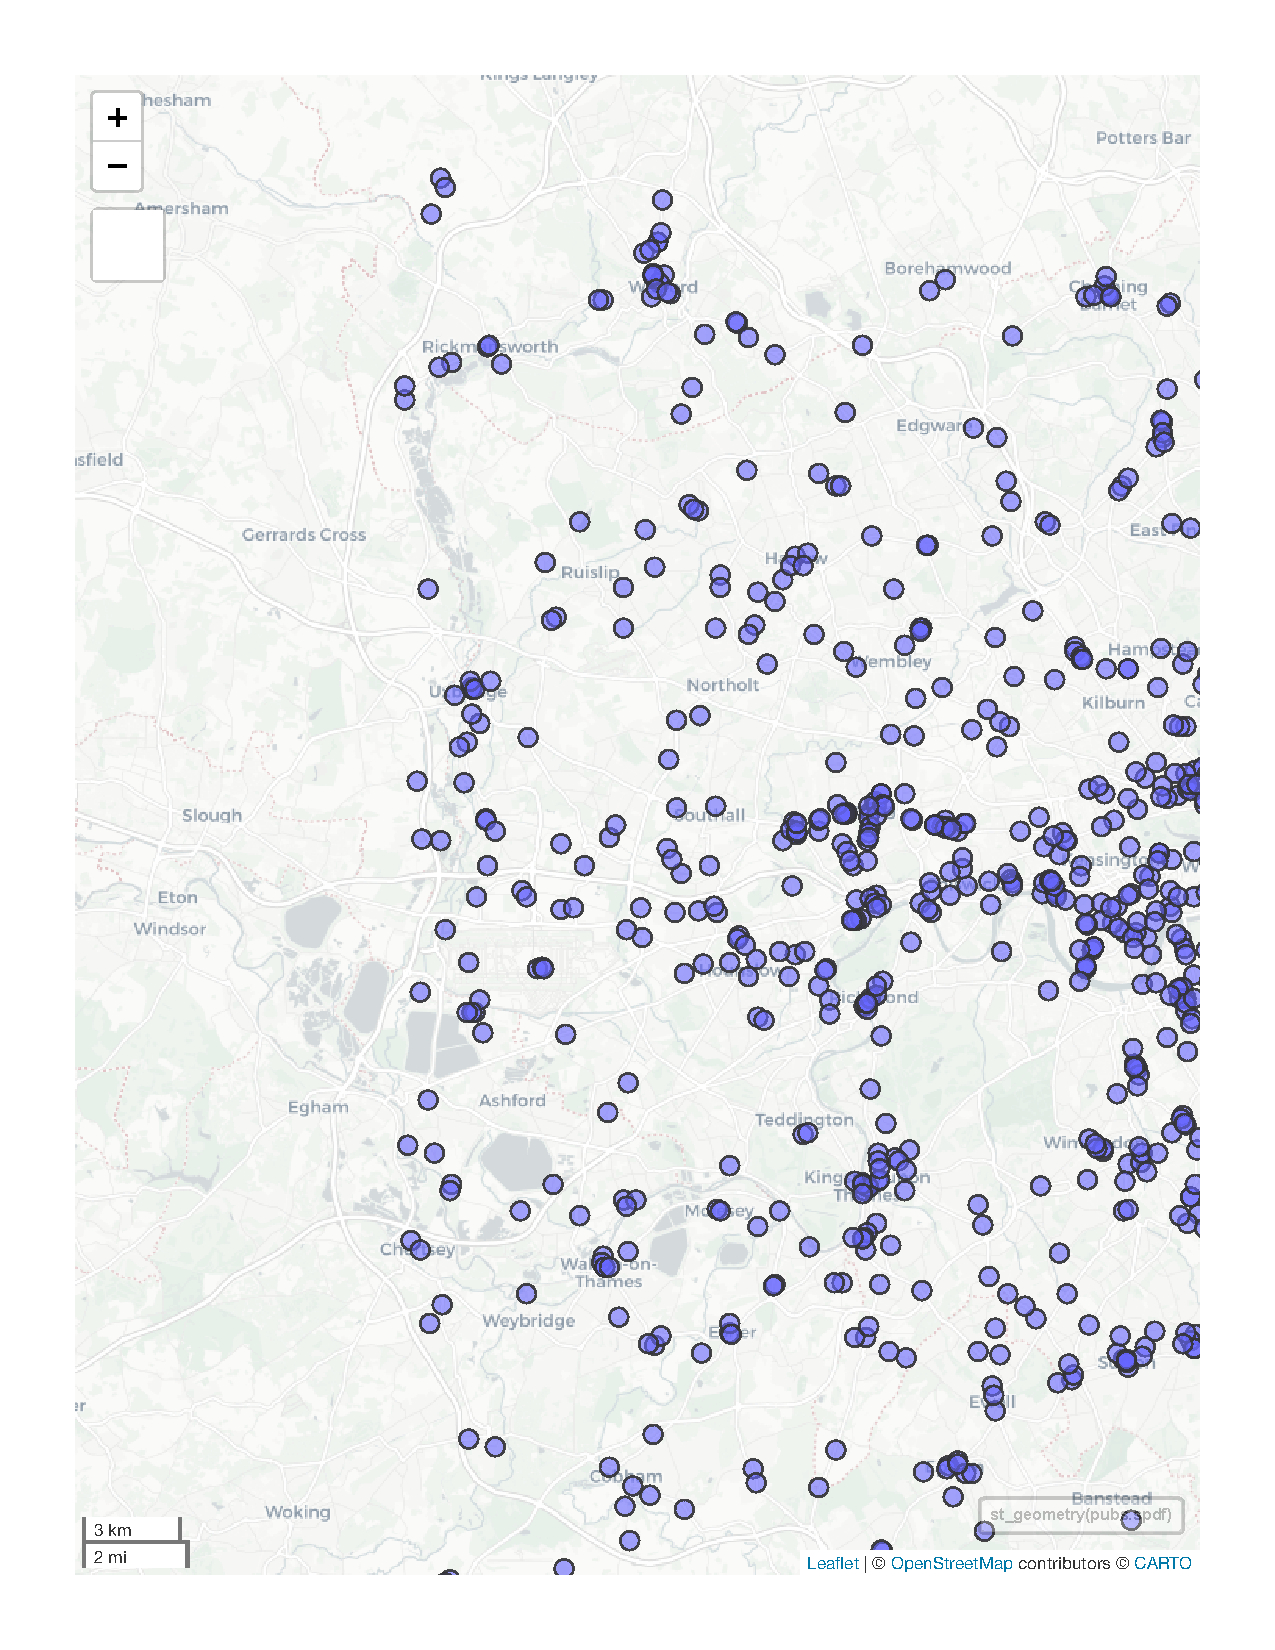
\includegraphics{01_refresher_files/figure-pdf/unnamed-chunk-19-1.pdf}

}

\end{figure}

Note that OSM is solely based on contribution by users, and the
\textbf{quality of OSM data varies}. Usually data quality is better in
larger cities, and better for more stable features (such as hospitals,
train stations, highways) rahter than pubs or restaurants which
regularly appear and disappear. However, data from
\href{https://data.london.gov.uk/dataset/cultural-infrastructure-map}{London
Datastore} would indicate more pubs than what we find with OSM.

\hypertarget{save}{%
\subsection{Save}\label{save}}

We will store the created data to use them again in the next session.

\begin{Shaded}
\begin{Highlighting}[]
\FunctionTok{save}\NormalTok{(msoa.spdf, }\AttributeTok{file =} \StringTok{"\_data/msoa\_spatial.RData"}\NormalTok{)}
\FunctionTok{save}\NormalTok{(ulez.spdf, }\AttributeTok{file =} \StringTok{"\_data/ulez\_spatial.RData"}\NormalTok{)}
\FunctionTok{save}\NormalTok{(pol.spdf, }\AttributeTok{file =} \StringTok{"\_data/pollution\_spatial.RData"}\NormalTok{)}
\FunctionTok{save}\NormalTok{(pubs.spdf, }\AttributeTok{file =} \StringTok{"\_data/pubs\_spatial.RData"}\NormalTok{)}
\end{Highlighting}
\end{Shaded}

\bookmarksetup{startatroot}

\hypertarget{data-manipulation-visualization}{%
\chapter{Data Manipulation \&
Visualization}\label{data-manipulation-visualization}}

\hypertarget{required-packages-1}{%
\subsection*{Required packages}\label{required-packages-1}}
\addcontentsline{toc}{subsection}{Required packages}

\begin{Shaded}
\begin{Highlighting}[]
\NormalTok{pkgs }\OtherTok{\textless{}{-}} \FunctionTok{c}\NormalTok{(}\StringTok{"sf"}\NormalTok{, }\StringTok{"gstat"}\NormalTok{, }\StringTok{"mapview"}\NormalTok{, }\StringTok{"nngeo"}\NormalTok{, }\StringTok{"rnaturalearth"}\NormalTok{, }\StringTok{"dplyr"}\NormalTok{,}
          \StringTok{"nomisr"}\NormalTok{, }\StringTok{"osmdata"}\NormalTok{, }\StringTok{"OpenStreetMap"}\NormalTok{, }\StringTok{"tidyr"}\NormalTok{, }\StringTok{"texreg"}\NormalTok{, }\StringTok{"downlit"}\NormalTok{, }\StringTok{"xml2"}\NormalTok{) }
\FunctionTok{lapply}\NormalTok{(pkgs, require, }\AttributeTok{character.only =} \ConstantTok{TRUE}\NormalTok{)}
\end{Highlighting}
\end{Shaded}

For mapping

\begin{Shaded}
\begin{Highlighting}[]
\NormalTok{pkgs }\OtherTok{\textless{}{-}} \FunctionTok{c}\NormalTok{(}\StringTok{"tmap"}\NormalTok{, }\StringTok{"tmaptools"}\NormalTok{, }\StringTok{"viridisLite"}\NormalTok{, }
          \StringTok{"ggplot2"}\NormalTok{, }\StringTok{"ggthemes"}\NormalTok{, }\StringTok{"rmapshaper"}\NormalTok{, }\StringTok{"cowplot"}\NormalTok{) }
\FunctionTok{lapply}\NormalTok{(pkgs, require, }\AttributeTok{character.only =} \ConstantTok{TRUE}\NormalTok{)}
\end{Highlighting}
\end{Shaded}

\hypertarget{session-info-1}{%
\subsection*{Session info}\label{session-info-1}}
\addcontentsline{toc}{subsection}{Session info}

\begin{Shaded}
\begin{Highlighting}[]
\FunctionTok{sessionInfo}\NormalTok{()}
\end{Highlighting}
\end{Shaded}

\begin{verbatim}
R version 4.4.1 (2024-06-14 ucrt)
Platform: x86_64-w64-mingw32/x64
Running under: Windows 11 x64 (build 22631)

Matrix products: default


locale:
[1] LC_COLLATE=English_United Kingdom.utf8 
[2] LC_CTYPE=English_United Kingdom.utf8   
[3] LC_MONETARY=English_United Kingdom.utf8
[4] LC_NUMERIC=C                           
[5] LC_TIME=English_United Kingdom.utf8    

time zone: Europe/Berlin
tzcode source: internal

attached base packages:
[1] stats     graphics  grDevices utils     datasets  methods   base     

other attached packages:
 [1] cowplot_1.1.3       rmapshaper_0.5.0    ggthemes_5.1.0     
 [4] ggplot2_3.5.1       viridisLite_0.4.2   tmaptools_3.1-1    
 [7] tmap_3.3-4          xml2_1.3.6          downlit_0.4.4      
[10] texreg_1.39.3       tidyr_1.3.1         OpenStreetMap_0.4.0
[13] osmdata_0.2.5       nomisr_0.4.7        dplyr_1.1.4        
[16] rnaturalearth_1.0.1 nngeo_0.4.8         mapview_2.11.2     
[19] gstat_2.1-1         sf_1.0-16          

loaded via a namespace (and not attached):
 [1] tidyselect_1.2.1   fastmap_1.2.0      leaflet_2.2.2      XML_3.99-0.16.1   
 [5] digest_0.6.35      lifecycle_1.0.4    terra_1.7-78       magrittr_2.0.3    
 [9] compiler_4.4.1     rlang_1.1.4        tools_4.4.1        utf8_1.2.4        
[13] rsdmx_0.6-3        data.table_1.15.4  knitr_1.47         FNN_1.1.4         
[17] htmlwidgets_1.6.4  curl_5.2.1         sp_2.1-4           classInt_0.4-10   
[21] plyr_1.8.9         RColorBrewer_1.1-3 abind_1.4-5        KernSmooth_2.23-24
[25] withr_3.0.0        purrr_1.0.2        leafsync_0.1.0     grid_4.4.1        
[29] stats4_4.4.1       fansi_1.0.6        xts_0.14.0         e1071_1.7-14      
[33] leafem_0.2.3       colorspace_2.1-0   scales_1.3.0       dichromat_2.0-0.1 
[37] cli_3.6.2          rmarkdown_2.27     intervals_0.15.4   generics_0.1.3    
[41] rstudioapi_0.16.0  httr_1.4.7         DBI_1.2.3          cachem_1.1.0      
[45] proxy_0.4-27       stringr_1.5.1      stars_0.6-5        parallel_4.4.1    
[49] base64enc_0.1-3    vctrs_0.6.5        V8_4.4.2           jsonlite_1.8.8    
[53] crosstalk_1.2.1    units_0.8-5        glue_1.7.0         lwgeom_0.2-14     
[57] codetools_0.2-20   stringi_1.8.4      rJava_1.0-11       gtable_0.3.5      
[61] raster_3.6-26      munsell_0.5.1      tibble_3.2.1       pillar_1.9.0      
[65] htmltools_0.5.8.1  satellite_1.0.5    R6_2.5.1           evaluate_0.24.0   
[69] lattice_0.22-6     png_0.1-8          memoise_2.0.1      snakecase_0.11.1  
[73] class_7.3-22       Rcpp_1.0.12        spacetime_1.3-1    xfun_0.45         
[77] zoo_1.8-12         pkgconfig_2.0.3   
\end{verbatim}

\hypertarget{reload-data-from-pervious-session}{%
\subsection*{Reload data from pervious
session}\label{reload-data-from-pervious-session}}
\addcontentsline{toc}{subsection}{Reload data from pervious session}

\begin{Shaded}
\begin{Highlighting}[]
\FunctionTok{load}\NormalTok{(}\StringTok{"\_data/msoa\_spatial.RData"}\NormalTok{)}
\FunctionTok{load}\NormalTok{(}\StringTok{"\_data/ulez\_spatial.RData"}\NormalTok{)}
\FunctionTok{load}\NormalTok{(}\StringTok{"\_data/pollution\_spatial.RData"}\NormalTok{)}
\FunctionTok{load}\NormalTok{(}\StringTok{"\_data/pubs\_spatial.RData"}\NormalTok{)}
\end{Highlighting}
\end{Shaded}

\hypertarget{manipulation-and-linkage}{%
\section{Manipulation and linkage}\label{manipulation-and-linkage}}

Having data with geo-spatial information allows to perform a variety of
methods to manipulate and link different data sources. Commonly used
methods include 1) subsetting, 2) point-in-polygon operations, 3)
distance measures, 4) intersections or buffer methods.

The \href{https://r-spatial.github.io/sf/articles/}{online Vignettes of
the sf package} provide a comprehensive overview of the multiple ways of
spatial manipulations.

\hypertarget{check-if-data-is-on-common-projection}{%
\subsubsection{Check if data is on common
projection}\label{check-if-data-is-on-common-projection}}

\begin{Shaded}
\begin{Highlighting}[]
\FunctionTok{st\_crs}\NormalTok{(msoa.spdf) }\SpecialCharTok{==} \FunctionTok{st\_crs}\NormalTok{(pol.spdf)}
\end{Highlighting}
\end{Shaded}

\begin{verbatim}
[1] FALSE
\end{verbatim}

\begin{Shaded}
\begin{Highlighting}[]
\FunctionTok{st\_crs}\NormalTok{(msoa.spdf) }\SpecialCharTok{==} \FunctionTok{st\_crs}\NormalTok{(pubs.spdf)}
\end{Highlighting}
\end{Shaded}

\begin{verbatim}
[1] FALSE
\end{verbatim}

\begin{Shaded}
\begin{Highlighting}[]
\FunctionTok{st\_crs}\NormalTok{(msoa.spdf) }\SpecialCharTok{==} \FunctionTok{st\_crs}\NormalTok{(ulez.spdf)}
\end{Highlighting}
\end{Shaded}

\begin{verbatim}
[1] FALSE
\end{verbatim}

The spatial data files are on different projections. Before we can do
any spatial operations with them, we have to transform them into a
common projection.

\begin{Shaded}
\begin{Highlighting}[]
\CommentTok{\# MSOA in different crs {-}{-}\textgreater{} transform}
\NormalTok{pol.spdf }\OtherTok{\textless{}{-}} \FunctionTok{st\_transform}\NormalTok{(pol.spdf, }\AttributeTok{crs =} \FunctionTok{st\_crs}\NormalTok{(msoa.spdf))}
\NormalTok{pubs.spdf }\OtherTok{\textless{}{-}} \FunctionTok{st\_transform}\NormalTok{(pubs.spdf, }\AttributeTok{crs =} \FunctionTok{st\_crs}\NormalTok{(msoa.spdf))}
\NormalTok{ulez.spdf }\OtherTok{\textless{}{-}} \FunctionTok{st\_transform}\NormalTok{(ulez.spdf, }\AttributeTok{crs =} \FunctionTok{st\_crs}\NormalTok{(msoa.spdf))}


\CommentTok{\# Check if all geometries are valid, and make valid if needed}
\NormalTok{msoa.spdf }\OtherTok{\textless{}{-}} \FunctionTok{st\_make\_valid}\NormalTok{(msoa.spdf)}
\end{Highlighting}
\end{Shaded}

The \texttt{st\_make\_valid()} function can help if the spatial
geometries have some problems such as holes or points that don't match
exactly.

\hypertarget{subsetting}{%
\subsection{Subsetting}\label{subsetting}}

We can subset spatial data in a similar way as we subset conventional
data.frames or matrices. For instance, below we simply reduce the
pollution grid across the UK to observations in London only.

\begin{Shaded}
\begin{Highlighting}[]
\CommentTok{\# Subset to pollution estimates in London}
\NormalTok{pol\_sub.spdf }\OtherTok{\textless{}{-}}\NormalTok{ pol.spdf[msoa.spdf, ] }\CommentTok{\# or:}
\NormalTok{pol\_sub.spdf }\OtherTok{\textless{}{-}} \FunctionTok{st\_filter}\NormalTok{(pol.spdf, msoa.spdf)}
\FunctionTok{mapview}\NormalTok{(pol\_sub.spdf)}
\end{Highlighting}
\end{Shaded}

\begin{figure}[H]

{\centering 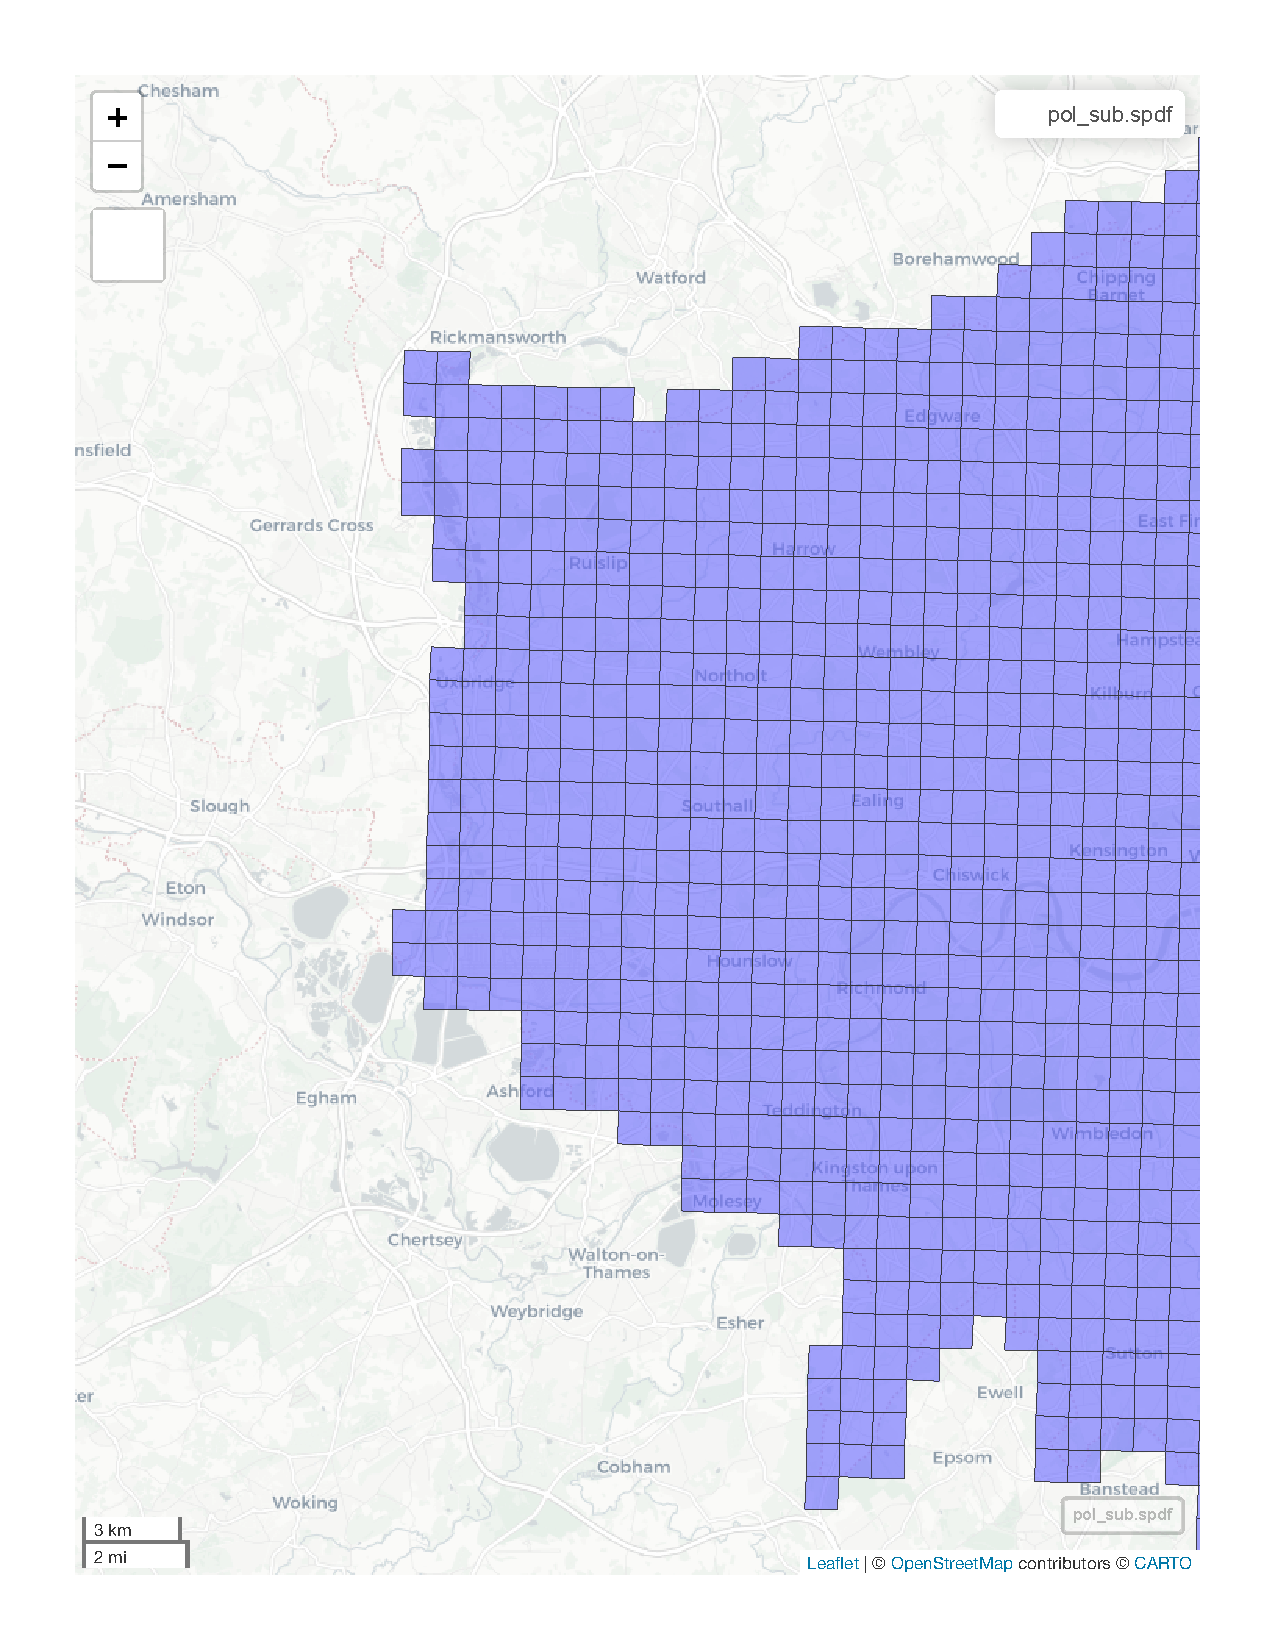
\includegraphics{02_spatial-data_files/figure-pdf/unnamed-chunk-7-1.pdf}

}

\end{figure}

Or we can reverse the above and exclude all intersecting units by
specifying \texttt{st\_disjoint} as alternative spatial operation using
the \texttt{op\ =} option (note the empty space for column selection).
\texttt{st\_filter()} with the \texttt{.predicate} option does the same
job. See the
\href{https://cran.r-project.org/web/packages/sf/vignettes/sf3.html}{sf
Vignette} for more operations.

\begin{Shaded}
\begin{Highlighting}[]
\CommentTok{\# Subset pubs to pubs not in the ulez area}
\NormalTok{sub2.spdf }\OtherTok{\textless{}{-}}\NormalTok{ pubs.spdf[ulez.spdf, , op }\OtherTok{=}\NormalTok{ st\_disjoint] }\CommentTok{\# or:}
\NormalTok{sub2.spdf }\OtherTok{\textless{}{-}} \FunctionTok{st\_filter}\NormalTok{(pubs.spdf, ulez.spdf, }\AttributeTok{.predicate =}\NormalTok{ st\_disjoint)}
\FunctionTok{mapview}\NormalTok{(sub2.spdf)}
\end{Highlighting}
\end{Shaded}

\begin{figure}[H]

{\centering 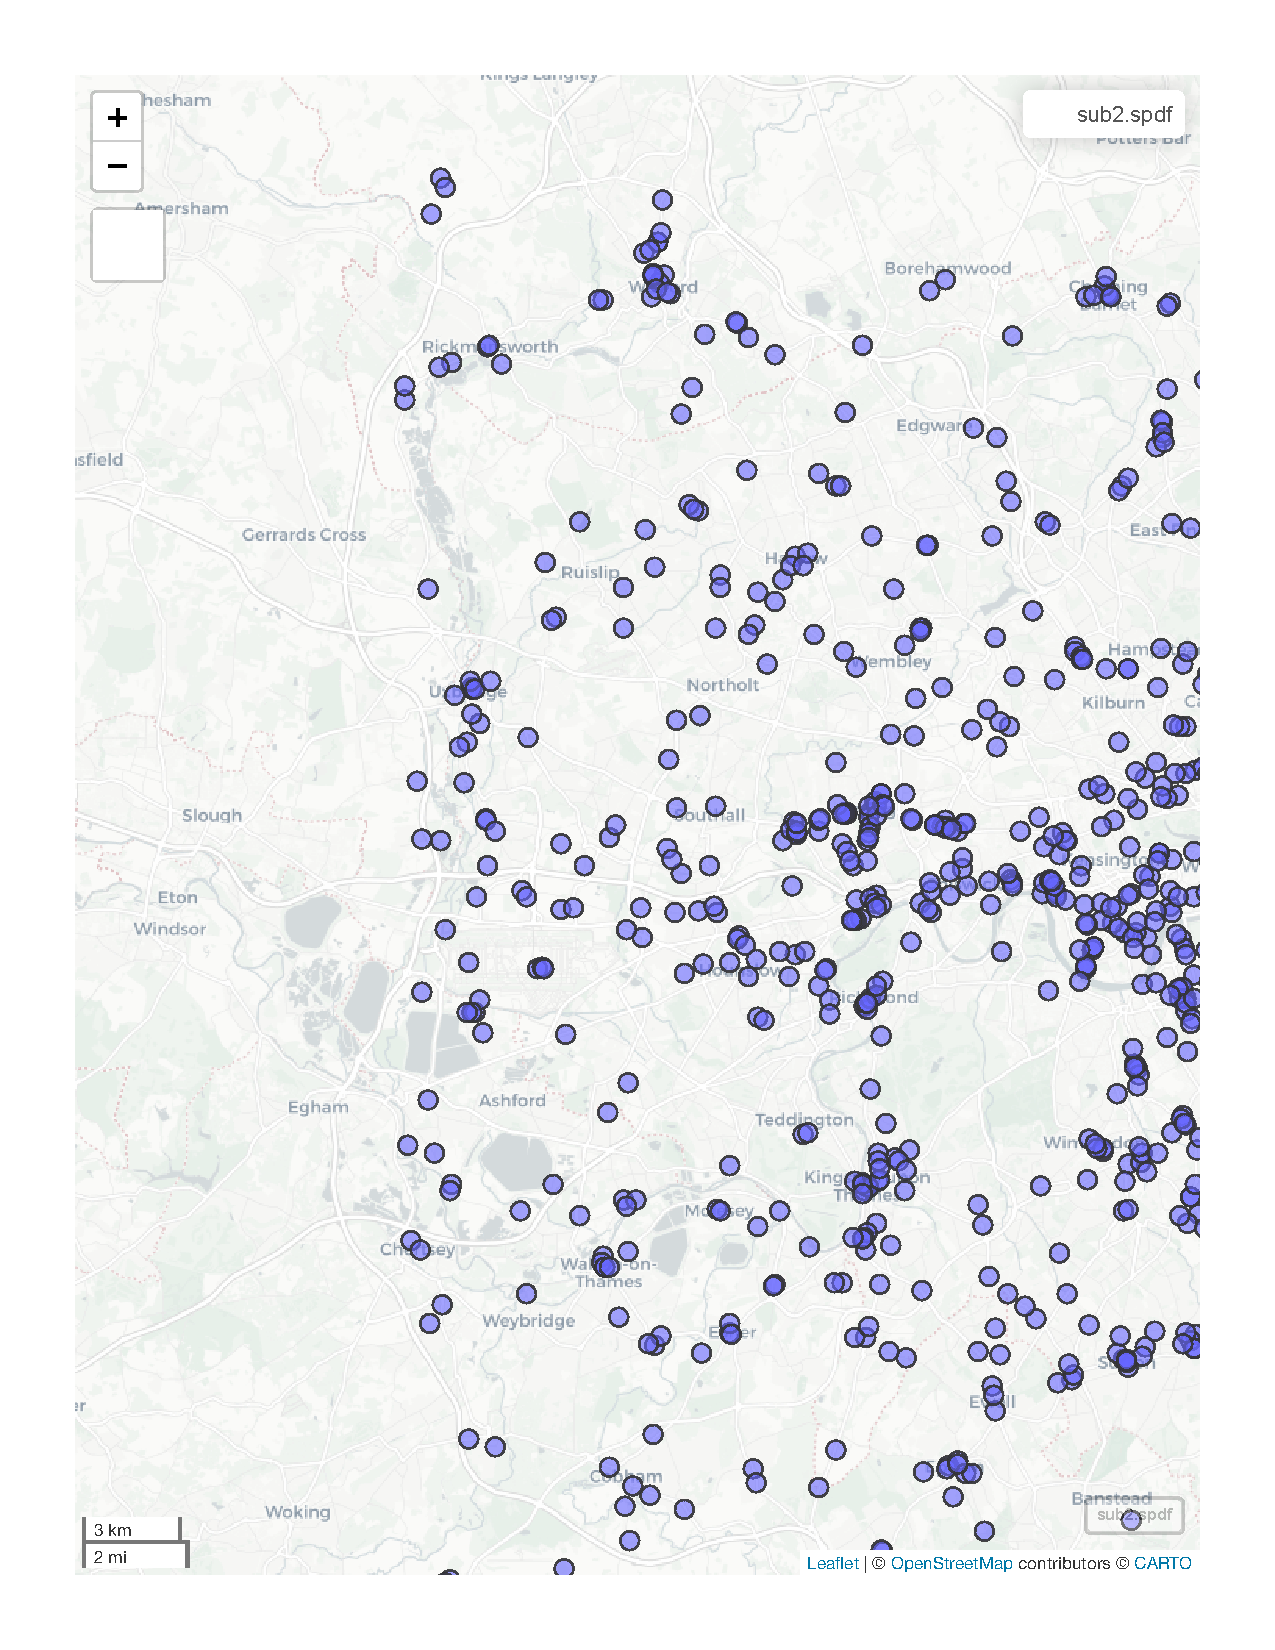
\includegraphics{02_spatial-data_files/figure-pdf/unnamed-chunk-8-1.pdf}

}

\end{figure}

We can easily create indicators of whether an MSOA is within ulez or
not.

\begin{Shaded}
\begin{Highlighting}[]
\NormalTok{msoa.spdf}\SpecialCharTok{$}\NormalTok{ulez }\OtherTok{\textless{}{-}} \DecValTok{0}

\CommentTok{\# intersecting lsoas}
\NormalTok{within }\OtherTok{\textless{}{-}}\NormalTok{ msoa.spdf[ulez.spdf,]}

\CommentTok{\# use their ids to create binary indicator }
\NormalTok{msoa.spdf}\SpecialCharTok{$}\NormalTok{ulez[}\FunctionTok{which}\NormalTok{(msoa.spdf}\SpecialCharTok{$}\NormalTok{MSOA11CD }\SpecialCharTok{\%in\%}\NormalTok{ within}\SpecialCharTok{$}\NormalTok{MSOA11CD)] }\OtherTok{\textless{}{-}} \DecValTok{1}
\FunctionTok{table}\NormalTok{(msoa.spdf}\SpecialCharTok{$}\NormalTok{ulez)}
\end{Highlighting}
\end{Shaded}

\begin{verbatim}

  0   1 
955  28 
\end{verbatim}

\hypertarget{point-in-polygon}{%
\subsection{Point in polygon}\label{point-in-polygon}}

We are interested in the number of pubs in each MSOA. So, we count the
number of points in each polygon.

\begin{Shaded}
\begin{Highlighting}[]
\CommentTok{\# Assign MSOA to each point}
\NormalTok{pubs\_msoa.join }\OtherTok{\textless{}{-}} \FunctionTok{st\_join}\NormalTok{(pubs.spdf, msoa.spdf, }\AttributeTok{join =}\NormalTok{ st\_within)}

\CommentTok{\# Count N by MSOA code (drop geometry to speed up)}
\NormalTok{pubs\_msoa.join }\OtherTok{\textless{}{-}}\NormalTok{ dplyr}\SpecialCharTok{::}\FunctionTok{count}\NormalTok{(}\FunctionTok{st\_drop\_geometry}\NormalTok{(pubs\_msoa.join),}
                               \AttributeTok{MSOA11CD =}\NormalTok{ pubs\_msoa.join}\SpecialCharTok{$}\NormalTok{MSOA11CD,}
                               \AttributeTok{name =} \StringTok{"pubs\_count"}\NormalTok{)}
\FunctionTok{sum}\NormalTok{(pubs\_msoa.join}\SpecialCharTok{$}\NormalTok{pubs\_count)}
\end{Highlighting}
\end{Shaded}

\begin{verbatim}
[1] 1601
\end{verbatim}

\begin{Shaded}
\begin{Highlighting}[]
\CommentTok{\# Merge and replace NAs with zero (no matches, no pubs)}
\NormalTok{msoa.spdf }\OtherTok{\textless{}{-}} \FunctionTok{merge}\NormalTok{(msoa.spdf, pubs\_msoa.join,}
                   \AttributeTok{by =} \StringTok{"MSOA11CD"}\NormalTok{, }\AttributeTok{all.x =} \ConstantTok{TRUE}\NormalTok{)}
\NormalTok{msoa.spdf}\SpecialCharTok{$}\NormalTok{pubs\_count[}\FunctionTok{is.na}\NormalTok{(msoa.spdf}\SpecialCharTok{$}\NormalTok{pubs\_count)] }\OtherTok{\textless{}{-}} \DecValTok{0}
\end{Highlighting}
\end{Shaded}

\hypertarget{distance-measures}{%
\subsection{Distance measures}\label{distance-measures}}

We might be interested in the distance to the nearest pub. Here, we use
the package \texttt{nngeo} to find k nearest neighbours with the
respective distance.

\begin{Shaded}
\begin{Highlighting}[]
\CommentTok{\# Use geometric centroid of each MSOA}
\NormalTok{cent.sp }\OtherTok{\textless{}{-}} \FunctionTok{st\_centroid}\NormalTok{(msoa.spdf[, }\StringTok{"MSOA11CD"}\NormalTok{])}
\end{Highlighting}
\end{Shaded}

\begin{verbatim}
Warning: st_centroid assumes attributes are constant over geometries
\end{verbatim}

\begin{Shaded}
\begin{Highlighting}[]
\CommentTok{\# Get K nearest neighbour with distance}
\NormalTok{knb.dist }\OtherTok{\textless{}{-}} \FunctionTok{st\_nn}\NormalTok{(cent.sp, }
\NormalTok{                  pubs.spdf,}
                  \AttributeTok{k =} \DecValTok{1}\NormalTok{,             }\CommentTok{\# number of nearest neighbours}
                  \AttributeTok{returnDist =} \ConstantTok{TRUE}\NormalTok{, }\CommentTok{\# we also want the distance}
                  \AttributeTok{progress =} \ConstantTok{FALSE}\NormalTok{)}
\end{Highlighting}
\end{Shaded}

\begin{verbatim}
projected points
\end{verbatim}

\begin{Shaded}
\begin{Highlighting}[]
\NormalTok{msoa.spdf}\SpecialCharTok{$}\NormalTok{dist\_pubs }\OtherTok{\textless{}{-}} \FunctionTok{unlist}\NormalTok{(knb.dist}\SpecialCharTok{$}\NormalTok{dist)}
\FunctionTok{summary}\NormalTok{(msoa.spdf}\SpecialCharTok{$}\NormalTok{dist\_pubs)}
\end{Highlighting}
\end{Shaded}

\begin{verbatim}
    Min.  1st Qu.   Median     Mean  3rd Qu.     Max. 
   9.079  305.149  565.018  701.961  948.047 3735.478 
\end{verbatim}

\hypertarget{intersections-buffers}{%
\subsection{Intersections + Buffers}\label{intersections-buffers}}

We may also want the average pollution within 1 km radius around each
MSOA centroid. Note that it is usually better to use a ego-centric
method where you calculate the average within a distance rather than
using the characteristic of the intersecting cells only (B. A. Lee et
al. 2008; Mohai and Saha 2007).

Therefore, we first create a buffer with \texttt{st\_buffer()} around
each midpoint and subsequently use \texttt{st\_intersetion()} to
calculate the overlap.

\begin{Shaded}
\begin{Highlighting}[]
\CommentTok{\# Create buffer (1km radius)}
\NormalTok{cent.buf }\OtherTok{\textless{}{-}} \FunctionTok{st\_buffer}\NormalTok{(cent.sp, }
                      \AttributeTok{dist =} \DecValTok{1000}\NormalTok{) }\CommentTok{\# dist in meters}
\FunctionTok{mapview}\NormalTok{(cent.buf)}
\end{Highlighting}
\end{Shaded}

\begin{figure}[H]

{\centering 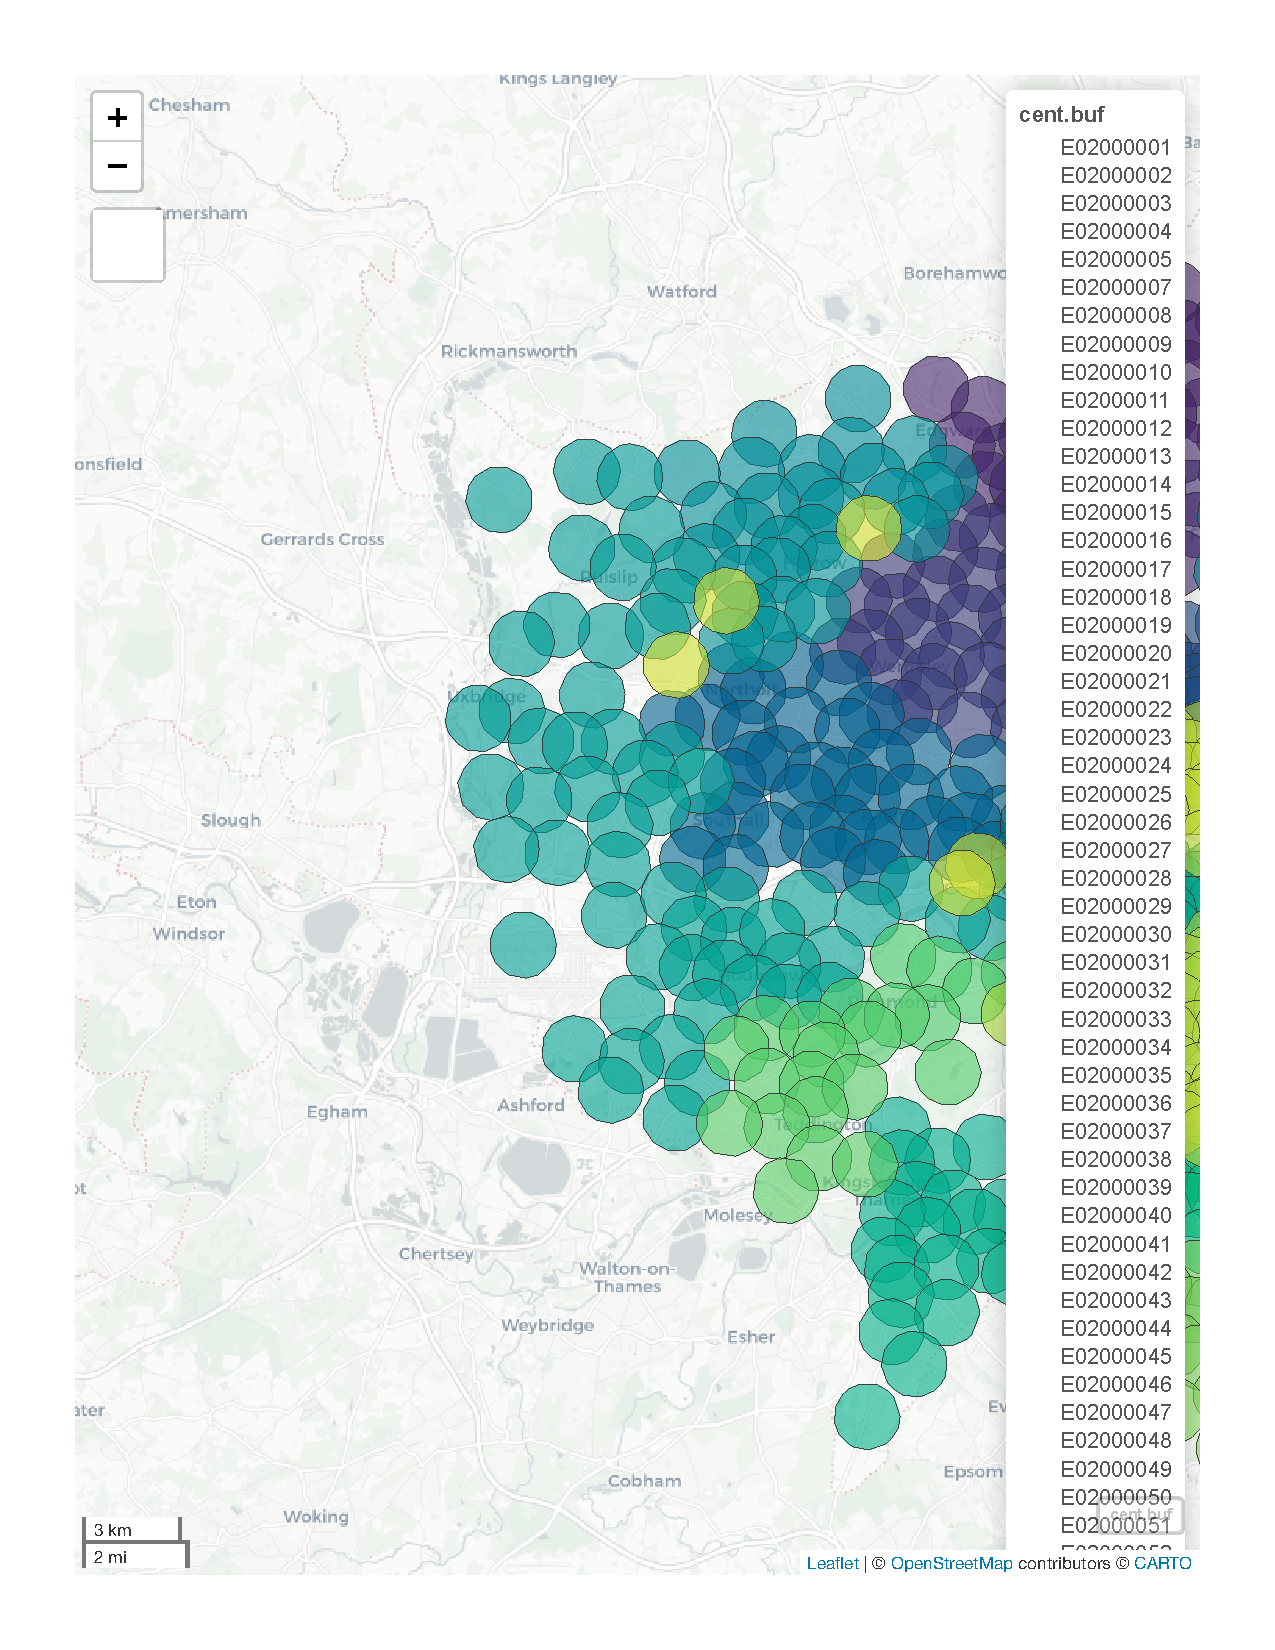
\includegraphics{02_spatial-data_files/figure-pdf/unnamed-chunk-12-1.pdf}

}

\end{figure}

\begin{Shaded}
\begin{Highlighting}[]
\CommentTok{\# Add area of each buffer (in this constant) }
\NormalTok{cent.buf}\SpecialCharTok{$}\NormalTok{area }\OtherTok{\textless{}{-}} \FunctionTok{as.numeric}\NormalTok{(}\FunctionTok{st\_area}\NormalTok{(cent.buf))}

\CommentTok{\# Calculate intersection of pollution grid and buffer}
\NormalTok{int.df }\OtherTok{\textless{}{-}} \FunctionTok{st\_intersection}\NormalTok{(cent.buf, pol.spdf)}
\end{Highlighting}
\end{Shaded}

\begin{verbatim}
Warning: attribute variables are assumed to be spatially constant throughout
all geometries
\end{verbatim}

\begin{Shaded}
\begin{Highlighting}[]
\NormalTok{int.df}\SpecialCharTok{$}\NormalTok{int\_area }\OtherTok{\textless{}{-}} \FunctionTok{as.numeric}\NormalTok{(}\FunctionTok{st\_area}\NormalTok{(int.df)) }\CommentTok{\# area of intersection}

\CommentTok{\# Area of intersection as share of buffer}
\NormalTok{int.df}\SpecialCharTok{$}\NormalTok{area\_per }\OtherTok{\textless{}{-}}\NormalTok{ int.df}\SpecialCharTok{$}\NormalTok{int\_area }\SpecialCharTok{/}\NormalTok{ int.df}\SpecialCharTok{$}\NormalTok{area}
\end{Highlighting}
\end{Shaded}

And we use the percent overlap areas as the weights to calculate a
weighted mean.

\begin{Shaded}
\begin{Highlighting}[]
\CommentTok{\# Aggregate as weighted mean}
\NormalTok{int.df }\OtherTok{\textless{}{-}} \FunctionTok{st\_drop\_geometry}\NormalTok{(int.df)}
\NormalTok{int.df}\SpecialCharTok{$}\NormalTok{no2\_weighted }\OtherTok{\textless{}{-}}\NormalTok{ int.df}\SpecialCharTok{$}\NormalTok{no22011 }\SpecialCharTok{*}\NormalTok{ int.df}\SpecialCharTok{$}\NormalTok{area\_per}
\NormalTok{int.df }\OtherTok{\textless{}{-}} \FunctionTok{aggregate}\NormalTok{(}\FunctionTok{list}\NormalTok{(}\AttributeTok{no2 =}\NormalTok{ int.df[, }\StringTok{"no2\_weighted"}\NormalTok{]), }
                    \AttributeTok{by =} \FunctionTok{list}\NormalTok{(}\AttributeTok{MSOA11CD =}\NormalTok{ int.df}\SpecialCharTok{$}\NormalTok{MSOA11CD),}
\NormalTok{                    sum)}

\CommentTok{\# Merge back to spatial data.frame}
\NormalTok{msoa.spdf }\OtherTok{\textless{}{-}} \FunctionTok{merge}\NormalTok{(msoa.spdf, int.df, }\AttributeTok{by =} \StringTok{"MSOA11CD"}\NormalTok{, }\AttributeTok{all.x =} \ConstantTok{TRUE}\NormalTok{)}

\FunctionTok{mapview}\NormalTok{(msoa.spdf[, }\StringTok{"no2"}\NormalTok{])}
\end{Highlighting}
\end{Shaded}

\begin{figure}[H]

{\centering 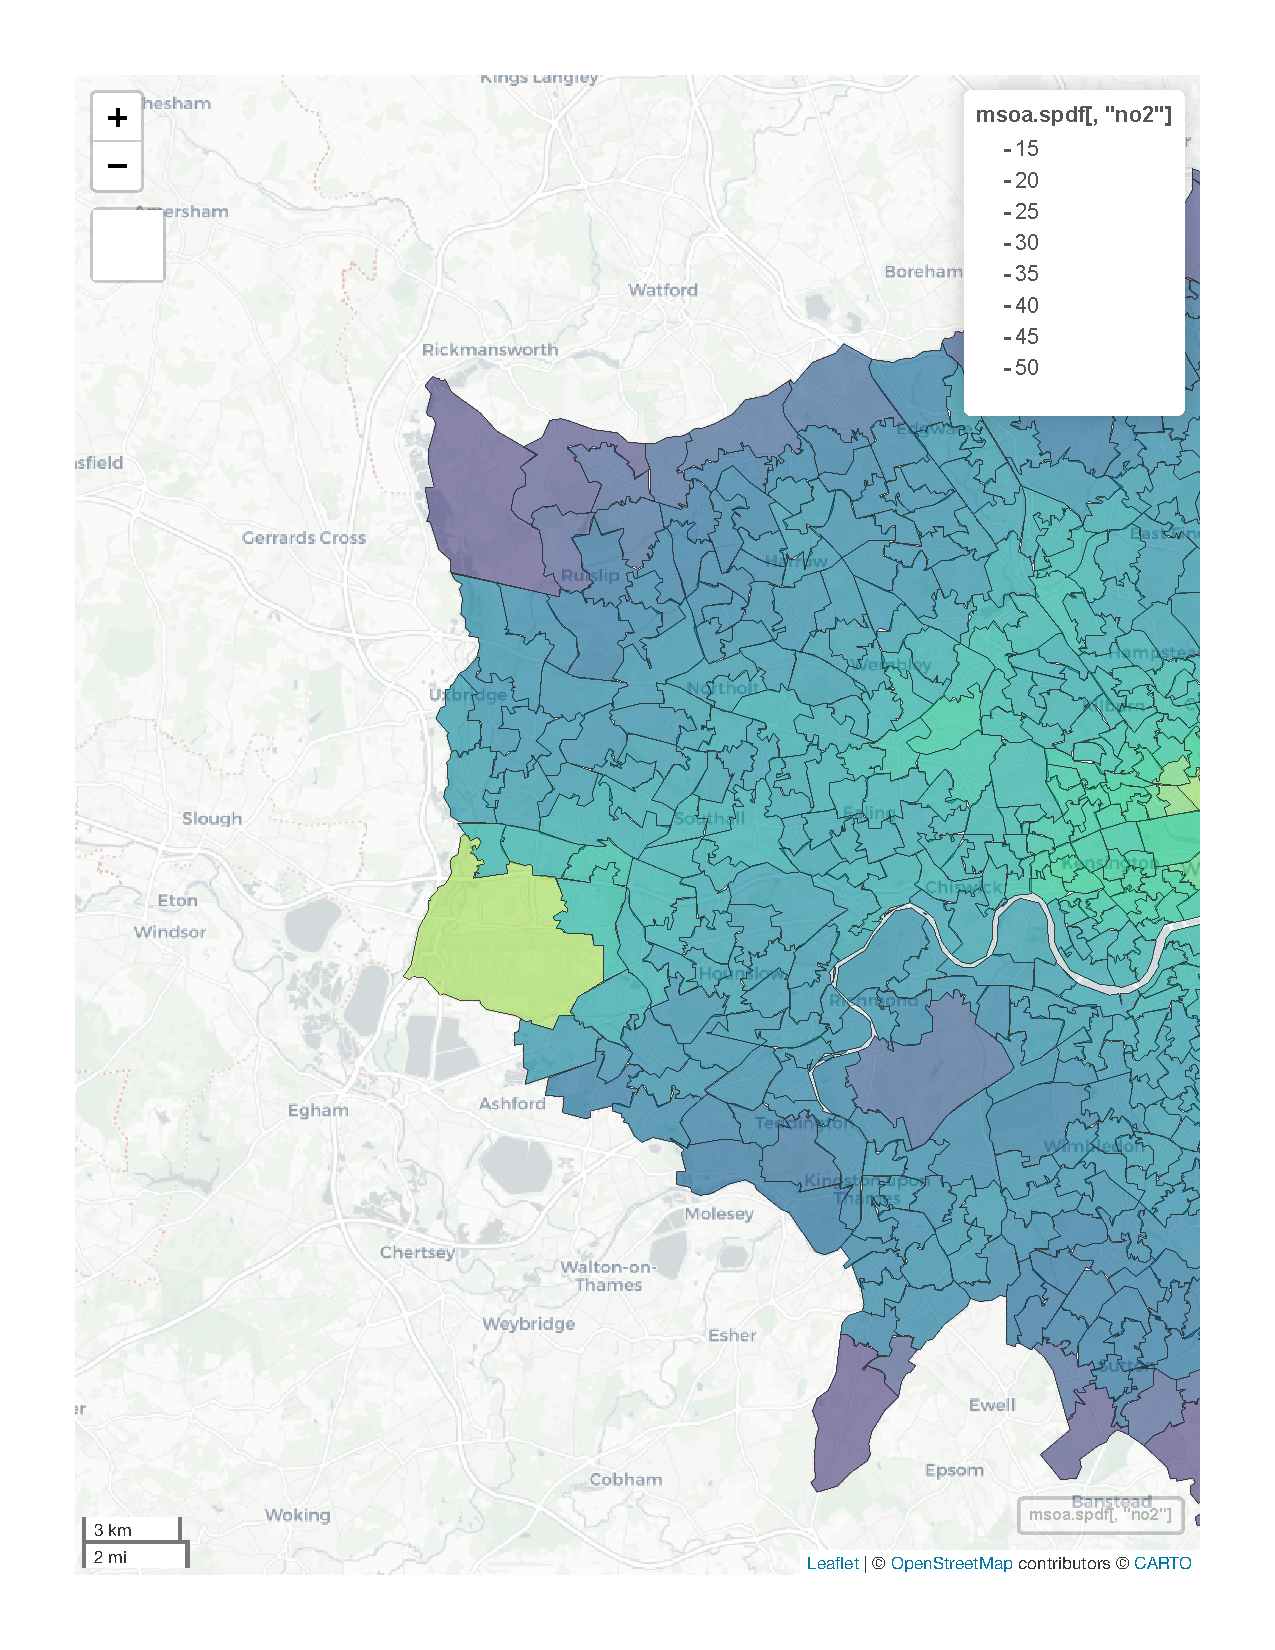
\includegraphics{02_spatial-data_files/figure-pdf/unnamed-chunk-13-1.pdf}

}

\end{figure}

Note: for buffer related methods, it often makes sense to use population
weighted centroids instead of geographic centroids (see
\href{https://geoportal.statistics.gov.uk/datasets/ons::middle-layer-super-output-areas-december-2011-population-weighted-centroids/about}{here}
for MSOA population weighted centroids). However, often this information
is not available.

\hypertarget{and-more}{%
\subsection{and more}\label{and-more}}

There are more spatial operation possible using sf. Have a look at the
\href{fig/sf.pdf}{sf Cheatsheet}.

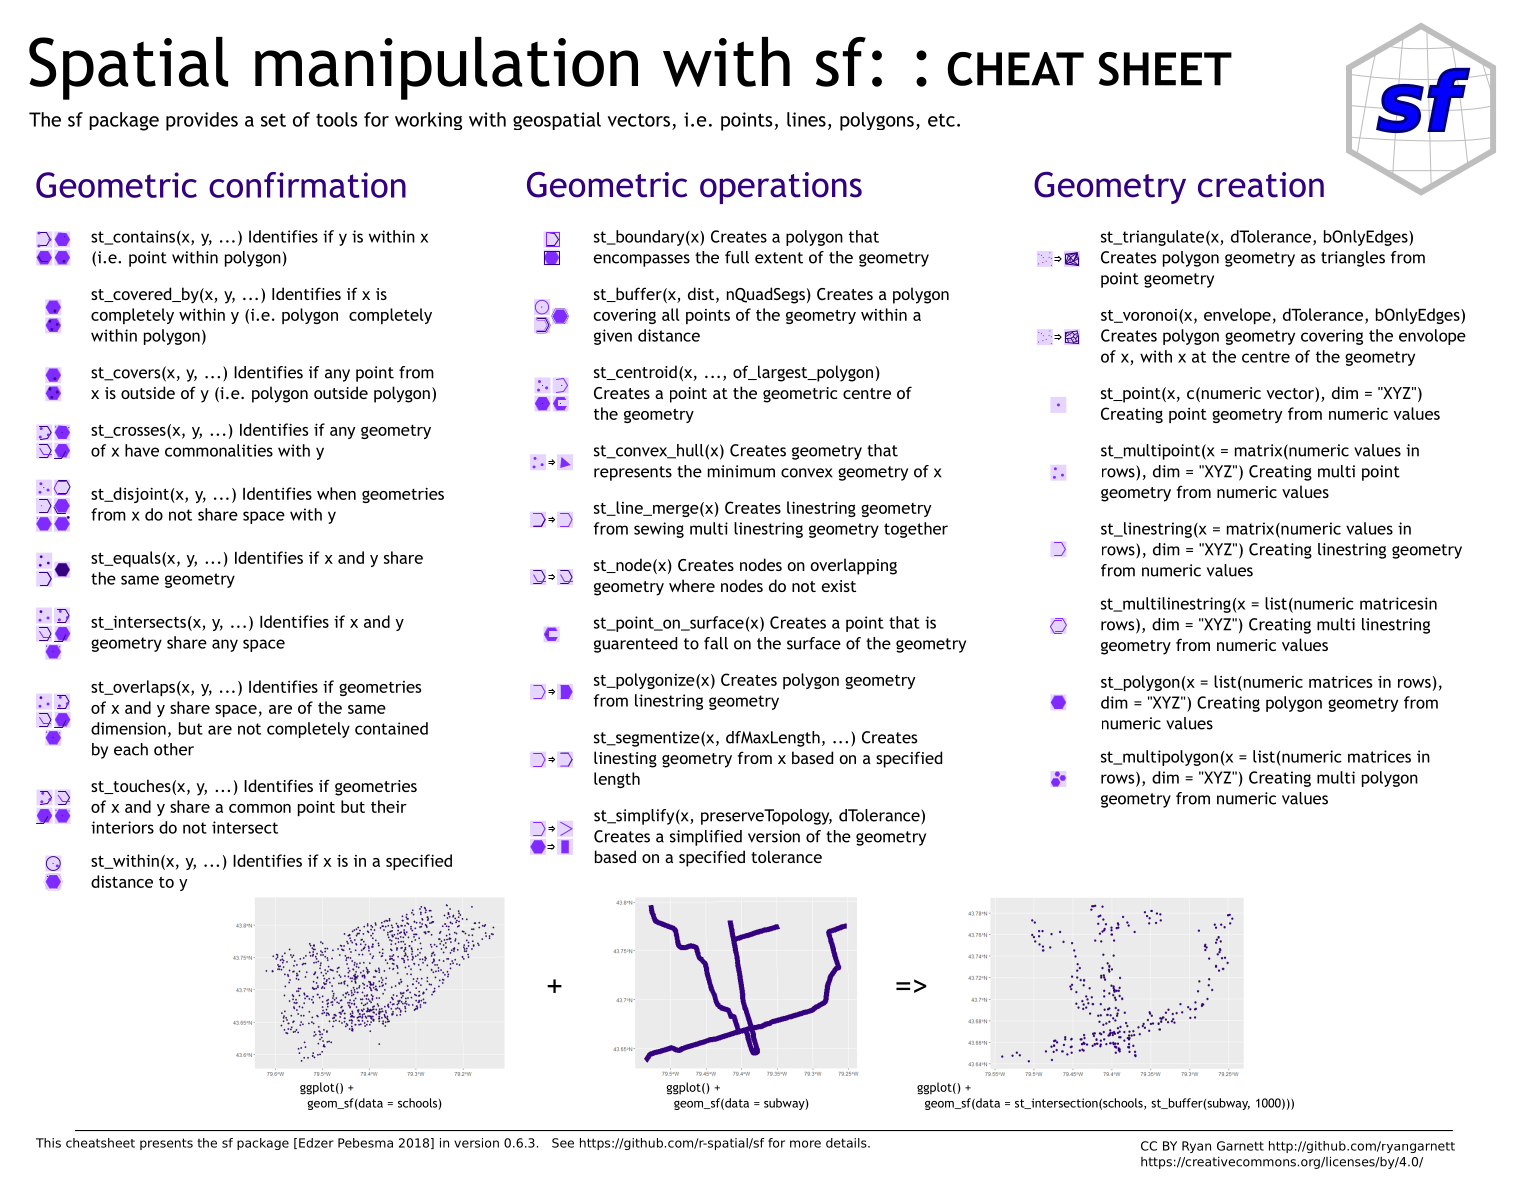
\includegraphics{fig/sf_1.png}

\hypertarget{air-pollution-and-ethnic-minorities}{%
\subsection{Air pollution and ethnic
minorities}\label{air-pollution-and-ethnic-minorities}}

With a few lines of code, we have compiled an original dataset
containing demographic information, air pollution, and some
infrastructural information.

Let's see what we can do with it.

\begin{Shaded}
\begin{Highlighting}[]
\CommentTok{\# Define ethnic group shares}
\NormalTok{msoa.spdf}\SpecialCharTok{$}\NormalTok{per\_mixed }\OtherTok{\textless{}{-}}\NormalTok{ msoa.spdf}\SpecialCharTok{$}\NormalTok{KS201EW\_200 }\SpecialCharTok{/}\NormalTok{ msoa.spdf}\SpecialCharTok{$}\NormalTok{KS201EW0001 }\SpecialCharTok{*} \DecValTok{100}
\NormalTok{msoa.spdf}\SpecialCharTok{$}\NormalTok{per\_asian }\OtherTok{\textless{}{-}}\NormalTok{ msoa.spdf}\SpecialCharTok{$}\NormalTok{KS201EW\_300 }\SpecialCharTok{/}\NormalTok{ msoa.spdf}\SpecialCharTok{$}\NormalTok{KS201EW0001 }\SpecialCharTok{*} \DecValTok{100}
\NormalTok{msoa.spdf}\SpecialCharTok{$}\NormalTok{per\_black }\OtherTok{\textless{}{-}}\NormalTok{ msoa.spdf}\SpecialCharTok{$}\NormalTok{KS201EW\_400 }\SpecialCharTok{/}\NormalTok{ msoa.spdf}\SpecialCharTok{$}\NormalTok{KS201EW0001 }\SpecialCharTok{*} \DecValTok{100}
\NormalTok{msoa.spdf}\SpecialCharTok{$}\NormalTok{per\_other }\OtherTok{\textless{}{-}}\NormalTok{ msoa.spdf}\SpecialCharTok{$}\NormalTok{KS201EW\_500 }\SpecialCharTok{/}\NormalTok{ msoa.spdf}\SpecialCharTok{$}\NormalTok{KS201EW0001 }\SpecialCharTok{*} \DecValTok{100}

\CommentTok{\# Define tenure}
\NormalTok{msoa.spdf}\SpecialCharTok{$}\NormalTok{per\_owner }\OtherTok{\textless{}{-}}\NormalTok{ msoa.spdf}\SpecialCharTok{$}\NormalTok{KS402EW\_100 }\SpecialCharTok{/}\NormalTok{ msoa.spdf}\SpecialCharTok{$}\NormalTok{KS402EW0001 }\SpecialCharTok{*} \DecValTok{100}
\NormalTok{msoa.spdf}\SpecialCharTok{$}\NormalTok{per\_social }\OtherTok{\textless{}{-}}\NormalTok{ msoa.spdf}\SpecialCharTok{$}\NormalTok{KS402EW\_200 }\SpecialCharTok{/}\NormalTok{ msoa.spdf}\SpecialCharTok{$}\NormalTok{KS402EW0001 }\SpecialCharTok{*} \DecValTok{100}

\CommentTok{\# Non British passport}
\NormalTok{msoa.spdf}\SpecialCharTok{$}\NormalTok{per\_nonUK }\OtherTok{\textless{}{-}}\NormalTok{ (msoa.spdf}\SpecialCharTok{$}\NormalTok{KS205EW0001 }\SpecialCharTok{{-}}\NormalTok{ msoa.spdf}\SpecialCharTok{$}\NormalTok{KS205EW0003)}\SpecialCharTok{/}\NormalTok{ msoa.spdf}\SpecialCharTok{$}\NormalTok{KS205EW0001 }\SpecialCharTok{*} \DecValTok{100}
\NormalTok{msoa.spdf}\SpecialCharTok{$}\NormalTok{per\_nonEU }\OtherTok{\textless{}{-}}\NormalTok{ (msoa.spdf}\SpecialCharTok{$}\NormalTok{KS205EW0001 }\SpecialCharTok{{-}}\NormalTok{ msoa.spdf}\SpecialCharTok{$}\NormalTok{KS205EW0003 }\SpecialCharTok{{-}}
\NormalTok{                          msoa.spdf}\SpecialCharTok{$}\NormalTok{KS205EW0004 }\SpecialCharTok{{-}}\NormalTok{ msoa.spdf}\SpecialCharTok{$}\NormalTok{KS205EW0005  }\SpecialCharTok{{-}} 
\NormalTok{                          msoa.spdf}\SpecialCharTok{$}\NormalTok{KS205EW0006)}\SpecialCharTok{/}\NormalTok{ msoa.spdf}\SpecialCharTok{$}\NormalTok{KS205EW0001 }\SpecialCharTok{*} \DecValTok{100}
\NormalTok{msoa.spdf}\SpecialCharTok{$}\NormalTok{per\_nonUK\_EU }\OtherTok{\textless{}{-}}\NormalTok{ (msoa.spdf}\SpecialCharTok{$}\NormalTok{KS205EW0005  }\SpecialCharTok{+}\NormalTok{ msoa.spdf}\SpecialCharTok{$}\NormalTok{KS205EW0006)}\SpecialCharTok{/}\NormalTok{ msoa.spdf}\SpecialCharTok{$}\NormalTok{KS205EW0001 }\SpecialCharTok{*} \DecValTok{100}


\CommentTok{\# Run regression}
\NormalTok{mod1.lm }\OtherTok{\textless{}{-}} \FunctionTok{lm}\NormalTok{(no2 }\SpecialCharTok{\textasciitilde{}}\NormalTok{ per\_mixed }\SpecialCharTok{+}\NormalTok{ per\_asian }\SpecialCharTok{+}\NormalTok{ per\_black }\SpecialCharTok{+}\NormalTok{ per\_other }\SpecialCharTok{+}
\NormalTok{                per\_owner }\SpecialCharTok{+}\NormalTok{ per\_social }\SpecialCharTok{+}\NormalTok{ pubs\_count }\SpecialCharTok{+}\NormalTok{ POPDEN }\SpecialCharTok{+}\NormalTok{ ulez,}
              \AttributeTok{data =}\NormalTok{ msoa.spdf)}

\CommentTok{\# summary}
\FunctionTok{screenreg}\NormalTok{(}\FunctionTok{list}\NormalTok{(mod1.lm), }\AttributeTok{digits =} \DecValTok{3}\NormalTok{)}
\end{Highlighting}
\end{Shaded}

\begin{verbatim}

========================
             Model 1    
------------------------
(Intercept)   37.112 ***
              (1.308)   
per_mixed     -0.090    
              (0.099)   
per_asian      0.018 *  
              (0.007)   
per_black     -0.085 ***
              (0.016)   
per_other      0.462 ***
              (0.047)   
per_owner     -0.207 ***
              (0.013)   
per_social    -0.058 ***
              (0.013)   
pubs_count     0.218 ***
              (0.040)   
POPDEN         0.037 ***
              (0.003)   
ulez           9.556 ***
              (0.686)   
------------------------
R^2            0.774    
Adj. R^2       0.772    
Num. obs.    983        
========================
*** p < 0.001; ** p < 0.01; * p < 0.05
\end{verbatim}

For some examples later, we also add data on house prices. We use the
median house prices in 2017 from the
\href{https://data.london.gov.uk/dataset/average-house-prices}{London
Datastore}.

\begin{Shaded}
\begin{Highlighting}[]
\CommentTok{\# Download}
\NormalTok{hp.link }\OtherTok{\textless{}{-}} \StringTok{"https://data.london.gov.uk/download/average{-}house{-}prices/bdf8eee7{-}41e1{-}4d24{-}90ce{-}93fe5cf040ae/land{-}registry{-}house{-}prices{-}MSOA.csv"}
\NormalTok{hp.df }\OtherTok{\textless{}{-}} \FunctionTok{read.csv}\NormalTok{(hp.link)}
\NormalTok{hp.df }\OtherTok{\textless{}{-}}\NormalTok{ hp.df[}\FunctionTok{which}\NormalTok{(hp.df}\SpecialCharTok{$}\NormalTok{Measure }\SpecialCharTok{==} \StringTok{"Median"} \SpecialCharTok{\&}
                       \FunctionTok{grepl}\NormalTok{(}\StringTok{"2011"}\NormalTok{, hp.df}\SpecialCharTok{$}\NormalTok{Year)), ]}
\FunctionTok{table}\NormalTok{(hp.df}\SpecialCharTok{$}\NormalTok{Year)}
\end{Highlighting}
\end{Shaded}

\begin{verbatim}

Year ending Dec 2011 Year ending Jun 2011 Year ending Mar 2011 
                 983                  983                  983 
Year ending Sep 2011 
                 983 
\end{verbatim}

\begin{Shaded}
\begin{Highlighting}[]
\CommentTok{\# Aggregate across 2011 values}
\NormalTok{hp.df}\SpecialCharTok{$}\NormalTok{med\_house\_price }\OtherTok{\textless{}{-}} \FunctionTok{as.numeric}\NormalTok{(hp.df}\SpecialCharTok{$}\NormalTok{Value)}
\NormalTok{hp.df }\OtherTok{\textless{}{-}} \FunctionTok{aggregate}\NormalTok{(hp.df[, }\StringTok{"med\_house\_price"}\NormalTok{, }\AttributeTok{drop =} \ConstantTok{FALSE}\NormalTok{],}
                   \AttributeTok{by =} \FunctionTok{list}\NormalTok{(}\AttributeTok{MSOA11CD =}\NormalTok{ hp.df}\SpecialCharTok{$}\NormalTok{Code),}
                   \AttributeTok{FUN =} \ControlFlowTok{function}\NormalTok{(x) }\FunctionTok{mean}\NormalTok{(x, }\AttributeTok{na.rm =} \ConstantTok{TRUE}\NormalTok{))}

\CommentTok{\# Merge spdf and housing prices}
\NormalTok{msoa.spdf }\OtherTok{\textless{}{-}} \FunctionTok{merge}\NormalTok{(msoa.spdf, hp.df,}
                   \AttributeTok{by =} \StringTok{"MSOA11CD"}\NormalTok{,}
                   \AttributeTok{all.x =} \ConstantTok{TRUE}\NormalTok{, }\AttributeTok{all.y =} \ConstantTok{FALSE}\NormalTok{)}
\FunctionTok{hist}\NormalTok{(}\FunctionTok{log}\NormalTok{(msoa.spdf}\SpecialCharTok{$}\NormalTok{med\_house\_price))}
\end{Highlighting}
\end{Shaded}

\begin{figure}[H]

{\centering 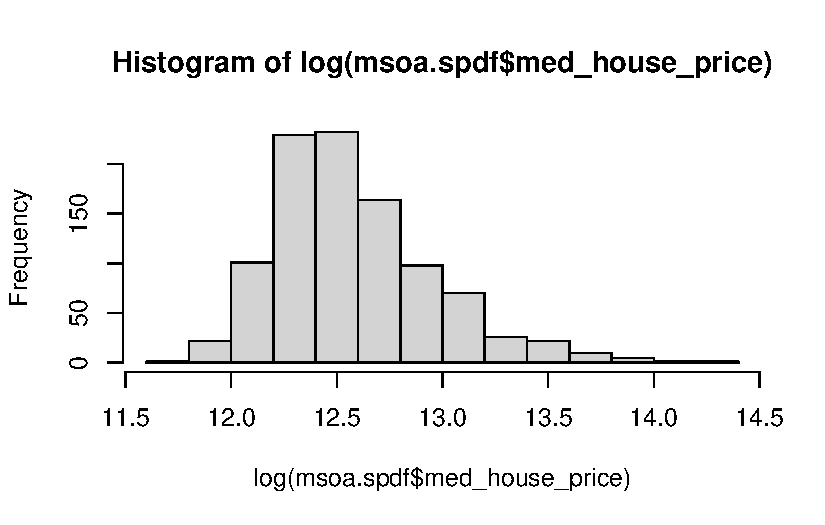
\includegraphics{02_spatial-data_files/figure-pdf/house-prices-1.pdf}

}

\end{figure}

\hypertarget{save-spatial-data}{%
\subsection{Save spatial data}\label{save-spatial-data}}

\begin{Shaded}
\begin{Highlighting}[]
\CommentTok{\# Save}
\FunctionTok{save}\NormalTok{(msoa.spdf, }\AttributeTok{file =} \StringTok{"\_data/msoa2\_spatial.RData"}\NormalTok{)}
\end{Highlighting}
\end{Shaded}

\hypertarget{visualization}{%
\section{Visualization}\label{visualization}}

A large advantage of spatial data is that different data sources can be
connected and combined. Another nice advantage is: you can create very
nice maps. And it's quite easy to do!
\href{https://stefanjuenger.github.io/}{Stefan Jünger} \&
\href{https://www.gesis.org/institut/mitarbeitendenverzeichnis/person/Anne-Kathrin.Stroppe}{Anne-Kathrin
Stroppe} provide more comprehensive materials on mapping in their
\href{https://github.com/StefanJuenger/gesis-workshop-geospatial-techniques-R-2023}{GESIS
workshop on geospatial techniques in R}.

Many packages and functions can be used to plot maps of spatial data.
For instance, ggplot as a function to plot spatial data using
\texttt{geom\_sf()}. I am personally a fan of \texttt{tmap}, which makes
many steps easier (but sometimes is less flexible).

A great tool for choosing coulour is for instance
\href{https://colorbrewer2.org/}{Colorbrewer}. \texttt{viridisLite}
provides another great resource to chose colours.

\hypertarget{tmaps}{%
\subsection{Tmaps}\label{tmaps}}

For instance, lets plot the NO2 estimates using tmap +
\texttt{tm\_fill()} (there are lots of alternatives like
\texttt{tm\_shape}, \texttt{tm\_points()}, \texttt{tm\_dots()}).

\begin{Shaded}
\begin{Highlighting}[]
\CommentTok{\# Define colours}
\NormalTok{cols }\OtherTok{\textless{}{-}} \FunctionTok{viridis}\NormalTok{(}\AttributeTok{n =} \DecValTok{7}\NormalTok{, }\AttributeTok{direction =} \DecValTok{1}\NormalTok{, }\AttributeTok{option =} \StringTok{"C"}\NormalTok{)}

\NormalTok{mp1 }\OtherTok{\textless{}{-}}  \FunctionTok{tm\_shape}\NormalTok{(msoa.spdf) }\SpecialCharTok{+} 
  \FunctionTok{tm\_fill}\NormalTok{(}\AttributeTok{col =} \StringTok{"no2"}\NormalTok{, }
          \AttributeTok{style =} \StringTok{"fisher"}\NormalTok{, }\CommentTok{\# algorithm to def cut points}
          \AttributeTok{n =} \DecValTok{7}\NormalTok{, }\CommentTok{\# Number of requested cut points}
          \AttributeTok{palette =}\NormalTok{ cols, }\CommentTok{\# colours}
          \AttributeTok{alpha =} \DecValTok{1}\NormalTok{, }\CommentTok{\# transparency }
          \AttributeTok{title =} \StringTok{"NO2"}\NormalTok{, }
          \AttributeTok{legend.hist =} \ConstantTok{FALSE} \CommentTok{\# histogram next to map?}
\NormalTok{          ) }\SpecialCharTok{+}
  \FunctionTok{tm\_borders}\NormalTok{(}\AttributeTok{col =} \StringTok{"white"}\NormalTok{, }\AttributeTok{lwd =} \FloatTok{0.5}\NormalTok{, }\AttributeTok{alpha =} \FloatTok{0.5}\NormalTok{) }

\NormalTok{mp1}
\end{Highlighting}
\end{Shaded}

\begin{figure}[H]

{\centering 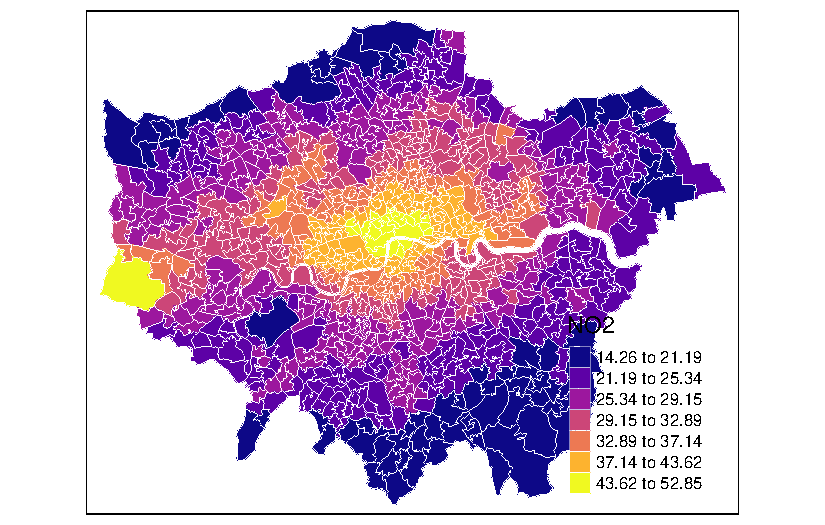
\includegraphics{02_spatial-data_files/figure-pdf/unnamed-chunk-16-1.pdf}

}

\end{figure}

Tmap allows to easily combine different objects by defining a new object
via \texttt{tm\_shape()}.

\begin{Shaded}
\begin{Highlighting}[]
\CommentTok{\# Define colours}
\NormalTok{cols }\OtherTok{\textless{}{-}} \FunctionTok{viridis}\NormalTok{(}\AttributeTok{n =} \DecValTok{7}\NormalTok{, }\AttributeTok{direction =} \DecValTok{1}\NormalTok{, }\AttributeTok{option =} \StringTok{"C"}\NormalTok{)}

\NormalTok{mp1 }\OtherTok{\textless{}{-}}  \FunctionTok{tm\_shape}\NormalTok{(msoa.spdf) }\SpecialCharTok{+} 
  \FunctionTok{tm\_fill}\NormalTok{(}\AttributeTok{col =} \StringTok{"no2"}\NormalTok{, }
          \AttributeTok{style =} \StringTok{"fisher"}\NormalTok{, }\CommentTok{\# algorithm to def cut points}
          \AttributeTok{n =} \DecValTok{7}\NormalTok{, }\CommentTok{\# Number of requested cut points}
          \AttributeTok{palette =}\NormalTok{ cols, }\CommentTok{\# colours}
          \AttributeTok{alpha =} \DecValTok{1}\NormalTok{, }\CommentTok{\# transparency }
          \AttributeTok{title =} \StringTok{"NO2"}\NormalTok{, }
          \AttributeTok{legend.hist =} \ConstantTok{FALSE} \CommentTok{\# histogram next to map?}
\NormalTok{          ) }\SpecialCharTok{+}
  \FunctionTok{tm\_borders}\NormalTok{(}\AttributeTok{col =} \StringTok{"white"}\NormalTok{, }\AttributeTok{lwd =} \FloatTok{0.5}\NormalTok{, }\AttributeTok{alpha =} \FloatTok{0.5}\NormalTok{) }\SpecialCharTok{+}
  \FunctionTok{tm\_shape}\NormalTok{(ulez.spdf) }\SpecialCharTok{+}
  \FunctionTok{tm\_borders}\NormalTok{(}\AttributeTok{col =} \StringTok{"red"}\NormalTok{, }\AttributeTok{lwd =} \DecValTok{1}\NormalTok{, }\AttributeTok{alpha =} \DecValTok{1}\NormalTok{) }

\NormalTok{mp1}
\end{Highlighting}
\end{Shaded}

\begin{figure}[H]

{\centering 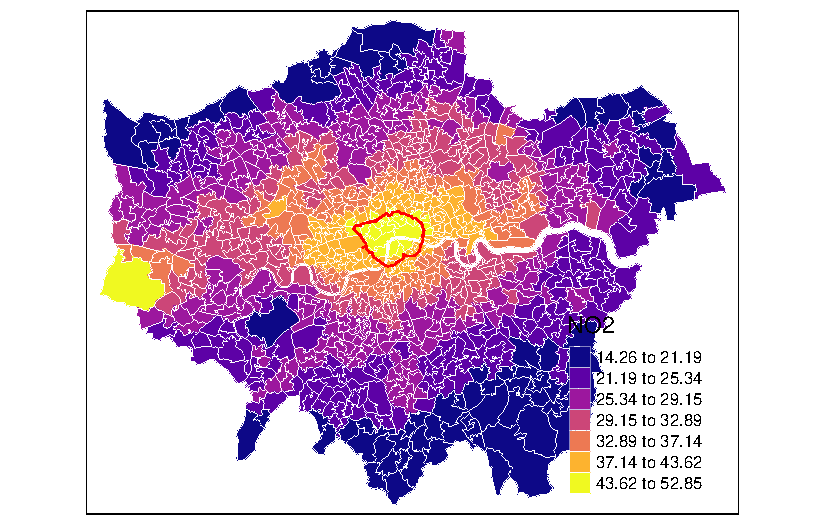
\includegraphics{02_spatial-data_files/figure-pdf/unnamed-chunk-17-1.pdf}

}

\end{figure}

And it is easy to change the layout.

\begin{Shaded}
\begin{Highlighting}[]
\CommentTok{\# Define colours}
\NormalTok{cols }\OtherTok{\textless{}{-}} \FunctionTok{viridis}\NormalTok{(}\AttributeTok{n =} \DecValTok{7}\NormalTok{, }\AttributeTok{direction =} \DecValTok{1}\NormalTok{, }\AttributeTok{option =} \StringTok{"C"}\NormalTok{)}

\NormalTok{mp1 }\OtherTok{\textless{}{-}}  \FunctionTok{tm\_shape}\NormalTok{(msoa.spdf) }\SpecialCharTok{+} 
  \FunctionTok{tm\_fill}\NormalTok{(}\AttributeTok{col =} \StringTok{"no2"}\NormalTok{, }
          \AttributeTok{style =} \StringTok{"fisher"}\NormalTok{, }\CommentTok{\# algorithm to def cut points}
          \AttributeTok{n =} \DecValTok{7}\NormalTok{, }\CommentTok{\# Number of requested cut points}
          \AttributeTok{palette =}\NormalTok{ cols, }\CommentTok{\# colours}
          \AttributeTok{alpha =} \DecValTok{1}\NormalTok{, }\CommentTok{\# transparency }
          \AttributeTok{title =} \FunctionTok{expression}\NormalTok{(}\StringTok{\textquotesingle{}in\textquotesingle{}}\SpecialCharTok{\textasciitilde{}}\NormalTok{mu}\SpecialCharTok{*}\StringTok{\textquotesingle{}g\textquotesingle{}}\SpecialCharTok{/}\NormalTok{m}\SpecialCharTok{\^{}}\NormalTok{\{}\DecValTok{3}\NormalTok{\}), }
          \AttributeTok{legend.hist =} \ConstantTok{FALSE} \CommentTok{\# histogram next to map?}
\NormalTok{          ) }\SpecialCharTok{+}
  \FunctionTok{tm\_borders}\NormalTok{(}\AttributeTok{col =} \StringTok{"white"}\NormalTok{, }\AttributeTok{lwd =} \FloatTok{0.5}\NormalTok{, }\AttributeTok{alpha =} \FloatTok{0.5}\NormalTok{) }\SpecialCharTok{+}
  \FunctionTok{tm\_shape}\NormalTok{(ulez.spdf) }\SpecialCharTok{+}
  \FunctionTok{tm\_borders}\NormalTok{(}\AttributeTok{col =} \StringTok{"red"}\NormalTok{, }\AttributeTok{lwd =} \DecValTok{1}\NormalTok{, }\AttributeTok{alpha =} \DecValTok{1}\NormalTok{) }\SpecialCharTok{+}
  \FunctionTok{tm\_layout}\NormalTok{(}\AttributeTok{frame =} \ConstantTok{FALSE}\NormalTok{,}
            \AttributeTok{legend.frame =} \ConstantTok{TRUE}\NormalTok{, }\AttributeTok{legend.bg.color =} \ConstantTok{TRUE}\NormalTok{,}
            \AttributeTok{legend.position =} \FunctionTok{c}\NormalTok{(}\StringTok{"right"}\NormalTok{, }\StringTok{"bottom"}\NormalTok{),}
            \AttributeTok{legend.outside =} \ConstantTok{FALSE}\NormalTok{,}
            \AttributeTok{main.title =} \StringTok{"NO2"}\NormalTok{, }
            \AttributeTok{main.title.position =} \StringTok{"center"}\NormalTok{,}
            \AttributeTok{main.title.size =} \FloatTok{1.6}\NormalTok{,}
            \AttributeTok{legend.title.size =} \FloatTok{0.8}\NormalTok{,}
            \AttributeTok{legend.text.size =} \FloatTok{0.8}\NormalTok{)}

\NormalTok{mp1}
\end{Highlighting}
\end{Shaded}

\begin{figure}[H]

{\centering 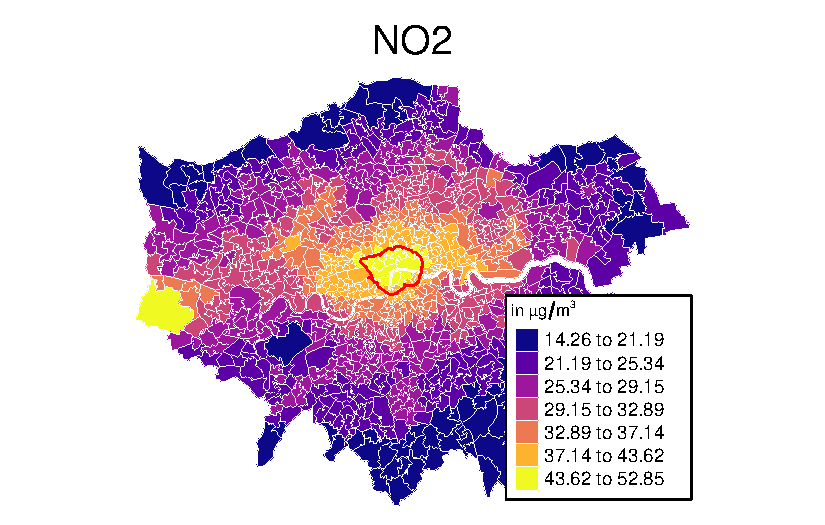
\includegraphics{02_spatial-data_files/figure-pdf/unnamed-chunk-18-1.pdf}

}

\end{figure}

We can also add some map information from OSM. However, it's sometimes a
bit tricky with the projection. That's why we switch into the OSM
projection here. Note that this osm query is build on retiring packages.

\begin{Shaded}
\begin{Highlighting}[]
\CommentTok{\# Save old projection}
\NormalTok{crs\_orig }\OtherTok{\textless{}{-}} \FunctionTok{st\_crs}\NormalTok{(msoa.spdf)}

\CommentTok{\# Change projection}
\NormalTok{ulez.spdf }\OtherTok{\textless{}{-}} \FunctionTok{st\_transform}\NormalTok{(ulez.spdf, }\DecValTok{4326}\NormalTok{)}
\NormalTok{msoa.spdf }\OtherTok{\textless{}{-}} \FunctionTok{st\_transform}\NormalTok{(msoa.spdf, }\DecValTok{4326}\NormalTok{)}

\CommentTok{\# Get OSM data for background}
\NormalTok{osm\_tmp }\OtherTok{\textless{}{-}} \FunctionTok{read\_osm}\NormalTok{(}\FunctionTok{st\_bbox}\NormalTok{(msoa.spdf), }\AttributeTok{ext =} \FloatTok{1.1}\NormalTok{, }\AttributeTok{type =} \StringTok{"osm{-}german"}\NormalTok{) }

\CommentTok{\# Define colours}
\NormalTok{cols }\OtherTok{\textless{}{-}} \FunctionTok{viridis}\NormalTok{(}\AttributeTok{n =} \DecValTok{7}\NormalTok{, }\AttributeTok{direction =} \DecValTok{1}\NormalTok{, }\AttributeTok{option =} \StringTok{"C"}\NormalTok{)}

\NormalTok{mp1 }\OtherTok{\textless{}{-}}  \FunctionTok{tm\_shape}\NormalTok{(osm\_tmp) }\SpecialCharTok{+} \FunctionTok{tm\_rgb}\NormalTok{() }\SpecialCharTok{+}
  \FunctionTok{tm\_shape}\NormalTok{(msoa.spdf) }\SpecialCharTok{+} 
  \FunctionTok{tm\_fill}\NormalTok{(}\AttributeTok{col =} \StringTok{"no2"}\NormalTok{, }
          \AttributeTok{style =} \StringTok{"fisher"}\NormalTok{, }\CommentTok{\# algorithm to def cut points}
          \AttributeTok{n =} \DecValTok{7}\NormalTok{, }\CommentTok{\# Number of requested cut points}
          \AttributeTok{palette =}\NormalTok{ cols, }\CommentTok{\# colours}
          \AttributeTok{alpha =} \FloatTok{0.8}\NormalTok{, }\CommentTok{\# transparency }
          \AttributeTok{title =} \FunctionTok{expression}\NormalTok{(}\StringTok{\textquotesingle{}in\textquotesingle{}}\SpecialCharTok{\textasciitilde{}}\NormalTok{mu}\SpecialCharTok{*}\StringTok{\textquotesingle{}g\textquotesingle{}}\SpecialCharTok{/}\NormalTok{m}\SpecialCharTok{\^{}}\NormalTok{\{}\DecValTok{3}\NormalTok{\}), }
          \AttributeTok{legend.hist =} \ConstantTok{FALSE} \CommentTok{\# histogram next to map?}
\NormalTok{          ) }\SpecialCharTok{+}
  \CommentTok{\#tm\_borders(col = "white", lwd = 0.5, alpha = 0.5) +}
  \FunctionTok{tm\_shape}\NormalTok{(ulez.spdf) }\SpecialCharTok{+}
  \FunctionTok{tm\_borders}\NormalTok{(}\AttributeTok{col =} \StringTok{"red"}\NormalTok{, }\AttributeTok{lwd =} \DecValTok{1}\NormalTok{, }\AttributeTok{alpha =} \DecValTok{1}\NormalTok{) }\SpecialCharTok{+}
  \FunctionTok{tm\_layout}\NormalTok{(}\AttributeTok{frame =} \ConstantTok{FALSE}\NormalTok{,}
            \AttributeTok{legend.frame =} \ConstantTok{TRUE}\NormalTok{, }\AttributeTok{legend.bg.color =} \ConstantTok{TRUE}\NormalTok{,}
            \AttributeTok{legend.position =} \FunctionTok{c}\NormalTok{(}\StringTok{"right"}\NormalTok{, }\StringTok{"bottom"}\NormalTok{),}
            \AttributeTok{legend.outside =} \ConstantTok{FALSE}\NormalTok{,}
            \AttributeTok{main.title =} \StringTok{"NO2"}\NormalTok{, }
            \AttributeTok{main.title.position =} \StringTok{"center"}\NormalTok{,}
            \AttributeTok{main.title.size =} \FloatTok{1.6}\NormalTok{,}
            \AttributeTok{legend.title.size =} \FloatTok{0.8}\NormalTok{,}
            \AttributeTok{legend.text.size =} \FloatTok{0.8}\NormalTok{)}

\NormalTok{mp1}
\end{Highlighting}
\end{Shaded}

\begin{figure}[H]

{\centering 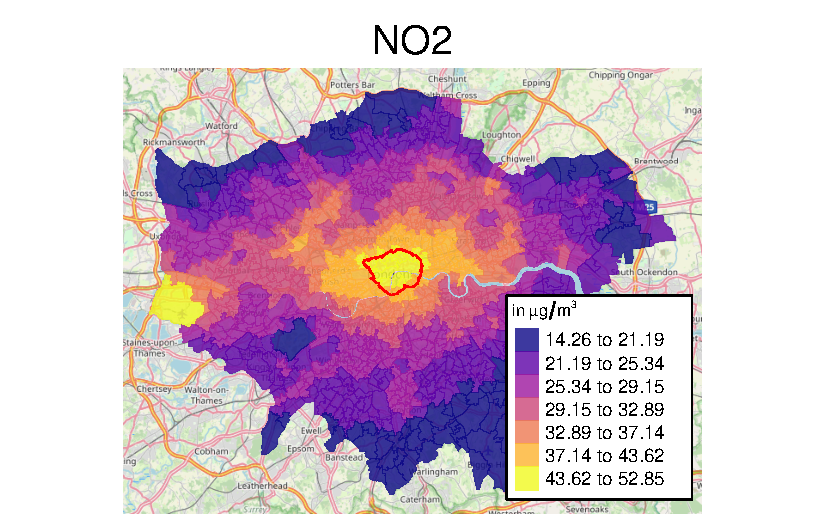
\includegraphics{02_spatial-data_files/figure-pdf/unnamed-chunk-19-1.pdf}

}

\end{figure}

Tmap also makes it easy to combine single maps

\begin{Shaded}
\begin{Highlighting}[]
\CommentTok{\# Define colours}
\NormalTok{cols1 }\OtherTok{\textless{}{-}} \FunctionTok{viridis}\NormalTok{(}\AttributeTok{n =} \DecValTok{7}\NormalTok{, }\AttributeTok{direction =} \DecValTok{1}\NormalTok{, }\AttributeTok{option =} \StringTok{"C"}\NormalTok{)}

\CommentTok{\# Define colours}
\NormalTok{cols2 }\OtherTok{\textless{}{-}} \FunctionTok{viridis}\NormalTok{(}\AttributeTok{n =} \DecValTok{7}\NormalTok{, }\AttributeTok{direction =} \DecValTok{1}\NormalTok{, }\AttributeTok{option =} \StringTok{"D"}\NormalTok{)}

\NormalTok{mp1 }\OtherTok{\textless{}{-}}  \FunctionTok{tm\_shape}\NormalTok{(osm\_tmp) }\SpecialCharTok{+} \FunctionTok{tm\_rgb}\NormalTok{() }\SpecialCharTok{+}
  \FunctionTok{tm\_shape}\NormalTok{(msoa.spdf) }\SpecialCharTok{+} 
  \FunctionTok{tm\_fill}\NormalTok{(}\AttributeTok{col =} \StringTok{"no2"}\NormalTok{, }
          \AttributeTok{style =} \StringTok{"fisher"}\NormalTok{, }\CommentTok{\# algorithm to def cut points}
          \AttributeTok{n =} \DecValTok{7}\NormalTok{, }\CommentTok{\# Number of requested cut points}
          \AttributeTok{palette =}\NormalTok{ cols1, }\CommentTok{\# colours}
          \AttributeTok{alpha =} \FloatTok{0.8}\NormalTok{, }\CommentTok{\# transparency }
          \AttributeTok{title =} \FunctionTok{expression}\NormalTok{(}\StringTok{\textquotesingle{}in\textquotesingle{}}\SpecialCharTok{\textasciitilde{}}\NormalTok{mu}\SpecialCharTok{*}\StringTok{\textquotesingle{}g\textquotesingle{}}\SpecialCharTok{/}\NormalTok{m}\SpecialCharTok{\^{}}\NormalTok{\{}\DecValTok{3}\NormalTok{\}), }
          \AttributeTok{legend.hist =} \ConstantTok{FALSE} \CommentTok{\# histogram next to map?}
\NormalTok{          ) }\SpecialCharTok{+}
  \CommentTok{\#tm\_borders(col = "white", lwd = 0.5, alpha = 0.5) +}
  \FunctionTok{tm\_shape}\NormalTok{(ulez.spdf) }\SpecialCharTok{+}
  \FunctionTok{tm\_borders}\NormalTok{(}\AttributeTok{col =} \StringTok{"red"}\NormalTok{, }\AttributeTok{lwd =} \DecValTok{1}\NormalTok{, }\AttributeTok{alpha =} \DecValTok{1}\NormalTok{) }\SpecialCharTok{+}
  \FunctionTok{tm\_layout}\NormalTok{(}\AttributeTok{frame =} \ConstantTok{FALSE}\NormalTok{,}
            \AttributeTok{legend.frame =} \ConstantTok{TRUE}\NormalTok{, }\AttributeTok{legend.bg.color =} \ConstantTok{TRUE}\NormalTok{,}
            \AttributeTok{legend.position =} \FunctionTok{c}\NormalTok{(}\StringTok{"right"}\NormalTok{, }\StringTok{"bottom"}\NormalTok{),}
            \AttributeTok{legend.outside =} \ConstantTok{FALSE}\NormalTok{,}
            \AttributeTok{main.title =} \StringTok{"NO2"}\NormalTok{, }
            \AttributeTok{main.title.position =} \StringTok{"center"}\NormalTok{,}
            \AttributeTok{main.title.size =} \FloatTok{1.4}\NormalTok{,}
            \AttributeTok{legend.title.size =} \FloatTok{0.8}\NormalTok{,}
            \AttributeTok{legend.text.size =} \FloatTok{0.8}\NormalTok{)}

\NormalTok{mp2 }\OtherTok{\textless{}{-}}  \FunctionTok{tm\_shape}\NormalTok{(osm\_tmp) }\SpecialCharTok{+} \FunctionTok{tm\_rgb}\NormalTok{() }\SpecialCharTok{+}
  \FunctionTok{tm\_shape}\NormalTok{(msoa.spdf) }\SpecialCharTok{+} 
  \FunctionTok{tm\_fill}\NormalTok{(}\AttributeTok{col =} \StringTok{"per\_black"}\NormalTok{, }
          \AttributeTok{style =} \StringTok{"fisher"}\NormalTok{, }\CommentTok{\# algorithm to def cut points}
          \AttributeTok{n =} \DecValTok{7}\NormalTok{, }\CommentTok{\# Number of requested cut points}
          \AttributeTok{palette =}\NormalTok{ cols2, }\CommentTok{\# colours}
          \AttributeTok{alpha =} \FloatTok{0.8}\NormalTok{, }\CommentTok{\# transparency }
          \AttributeTok{title =} \StringTok{"\% white"}\NormalTok{, }
          \AttributeTok{legend.hist =} \ConstantTok{FALSE} \CommentTok{\# histogram next to map?}
\NormalTok{          ) }\SpecialCharTok{+}
  \CommentTok{\#tm\_borders(col = "white", lwd = 0.5, alpha = 0.5) +}
  \FunctionTok{tm\_shape}\NormalTok{(ulez.spdf) }\SpecialCharTok{+}
  \FunctionTok{tm\_borders}\NormalTok{(}\AttributeTok{col =} \StringTok{"red"}\NormalTok{, }\AttributeTok{lwd =} \DecValTok{1}\NormalTok{, }\AttributeTok{alpha =} \DecValTok{1}\NormalTok{) }\SpecialCharTok{+}
  \FunctionTok{tm\_layout}\NormalTok{(}\AttributeTok{frame =} \ConstantTok{FALSE}\NormalTok{,}
            \AttributeTok{legend.frame =} \ConstantTok{TRUE}\NormalTok{, }\AttributeTok{legend.bg.color =} \ConstantTok{TRUE}\NormalTok{,}
            \AttributeTok{legend.position =} \FunctionTok{c}\NormalTok{(}\StringTok{"right"}\NormalTok{, }\StringTok{"bottom"}\NormalTok{),}
            \AttributeTok{legend.outside =} \ConstantTok{FALSE}\NormalTok{,}
            \AttributeTok{main.title =} \StringTok{"Ethnic Black inhabitants"}\NormalTok{, }
            \AttributeTok{main.title.position =} \StringTok{"center"}\NormalTok{,}
            \AttributeTok{main.title.size =} \FloatTok{1.4}\NormalTok{,}
            \AttributeTok{legend.title.size =} \FloatTok{0.8}\NormalTok{,}
            \AttributeTok{legend.text.size =} \FloatTok{0.8}\NormalTok{)}

\FunctionTok{tmap\_arrange}\NormalTok{(mp1, mp2, }\AttributeTok{ncol =} \DecValTok{2}\NormalTok{, }\AttributeTok{nrow =} \DecValTok{1}\NormalTok{)}
\end{Highlighting}
\end{Shaded}

\begin{verbatim}
Legend labels were too wide. The labels have been resized to 0.63, 0.63, 0.63, 0.63, 0.63, 0.63, 0.63. Increase legend.width (argument of tm_layout) to make the legend wider and therefore the labels larger.
\end{verbatim}

\begin{verbatim}
Some legend labels were too wide. These labels have been resized to 0.68, 0.63, 0.63, 0.63, 0.63. Increase legend.width (argument of tm_layout) to make the legend wider and therefore the labels larger.
\end{verbatim}

\begin{figure}[H]

{\centering 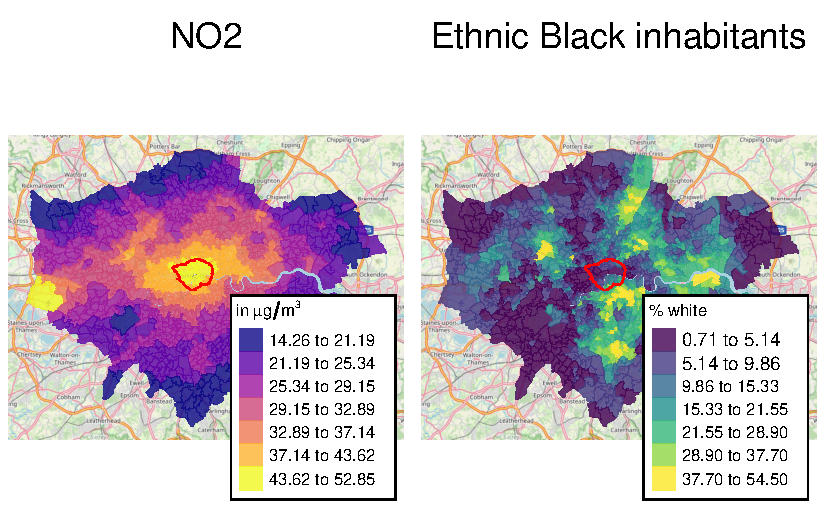
\includegraphics{02_spatial-data_files/figure-pdf/unnamed-chunk-20-1.pdf}

}

\end{figure}

And you can easily export those to png or pdf

\begin{Shaded}
\begin{Highlighting}[]
\FunctionTok{png}\NormalTok{(}\AttributeTok{file =} \FunctionTok{paste}\NormalTok{(}\StringTok{"London.png"}\NormalTok{, }\AttributeTok{sep =} \StringTok{""}\NormalTok{), }\AttributeTok{width =} \DecValTok{14}\NormalTok{, }\AttributeTok{height =} \DecValTok{7}\NormalTok{, }\AttributeTok{units =} \StringTok{"in"}\NormalTok{, }
    \AttributeTok{res =} \DecValTok{100}\NormalTok{, }\AttributeTok{bg =} \StringTok{"white"}\NormalTok{)}
\FunctionTok{par}\NormalTok{(}\AttributeTok{mar=}\FunctionTok{c}\NormalTok{(}\DecValTok{0}\NormalTok{,}\DecValTok{0}\NormalTok{,}\DecValTok{3}\NormalTok{,}\DecValTok{0}\NormalTok{))}
\FunctionTok{par}\NormalTok{(}\AttributeTok{mfrow=}\FunctionTok{c}\NormalTok{(}\DecValTok{1}\NormalTok{,}\DecValTok{1}\NormalTok{),}\AttributeTok{oma=}\FunctionTok{c}\NormalTok{(}\DecValTok{0}\NormalTok{,}\DecValTok{0}\NormalTok{,}\DecValTok{0}\NormalTok{,}\DecValTok{0}\NormalTok{))}
\FunctionTok{tmap\_arrange}\NormalTok{(mp1, mp2, }\AttributeTok{ncol =} \DecValTok{2}\NormalTok{, }\AttributeTok{nrow =} \DecValTok{1}\NormalTok{)}
\FunctionTok{dev.off}\NormalTok{()}
\end{Highlighting}
\end{Shaded}

\begin{verbatim}
pdf 
  2 
\end{verbatim}

\hypertarget{ggplot}{%
\subsection{ggplot}\label{ggplot}}

\begin{Shaded}
\begin{Highlighting}[]
\NormalTok{gp }\OtherTok{\textless{}{-}} \FunctionTok{ggplot}\NormalTok{(msoa.spdf)}\SpecialCharTok{+}
    \FunctionTok{geom\_sf}\NormalTok{(}\FunctionTok{aes}\NormalTok{(}\AttributeTok{fill =}\NormalTok{ no2))}\SpecialCharTok{+}
    \FunctionTok{scale\_fill\_viridis\_c}\NormalTok{(}\AttributeTok{option =} \StringTok{"B"}\NormalTok{)}\SpecialCharTok{+}
    \FunctionTok{coord\_sf}\NormalTok{(}\AttributeTok{datum =} \ConstantTok{NA}\NormalTok{)}\SpecialCharTok{+}
    \FunctionTok{theme\_map}\NormalTok{()}\SpecialCharTok{+}
    \FunctionTok{theme}\NormalTok{(}\AttributeTok{legend.position =} \FunctionTok{c}\NormalTok{(.}\DecValTok{9}\NormalTok{, .}\DecValTok{6}\NormalTok{))}
\end{Highlighting}
\end{Shaded}

\begin{verbatim}
Warning: A numeric `legend.position` argument in `theme()` was deprecated in ggplot2
3.5.0.
i Please use the `legend.position.inside` argument of `theme()` instead.
\end{verbatim}

\begin{Shaded}
\begin{Highlighting}[]
\NormalTok{gp}
\end{Highlighting}
\end{Shaded}

\begin{figure}[H]

{\centering 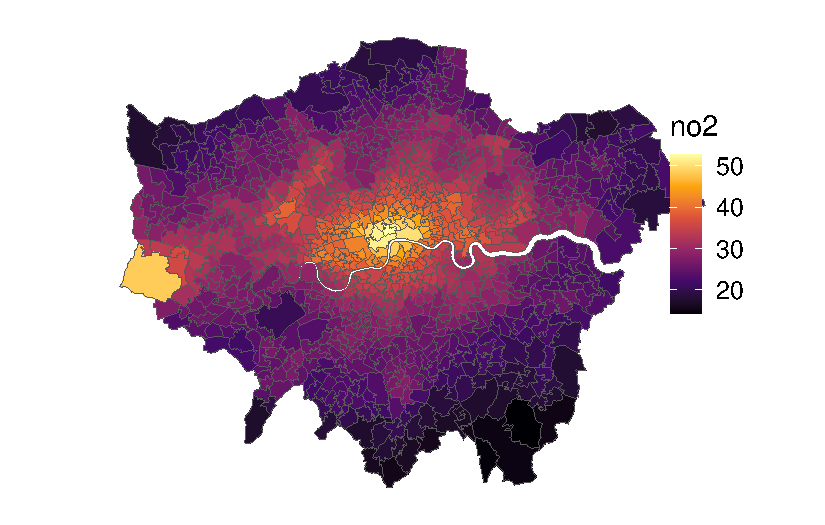
\includegraphics{02_spatial-data_files/figure-pdf/unnamed-chunk-22-1.pdf}

}

\end{figure}

\begin{Shaded}
\begin{Highlighting}[]
\CommentTok{\# Get some larger scale boundaries}
\NormalTok{borough.spdf }\OtherTok{\textless{}{-}} \FunctionTok{st\_read}\NormalTok{(}\AttributeTok{dsn =} \FunctionTok{paste0}\NormalTok{(}\StringTok{"\_data"}\NormalTok{, }\StringTok{"/statistical{-}gis{-}boundaries{-}london/ESRI"}\NormalTok{),}
                     \AttributeTok{layer =} \StringTok{"London\_Borough\_Excluding\_MHW"} \CommentTok{\# Note: no file ending}
\NormalTok{                     )}
\end{Highlighting}
\end{Shaded}

\begin{verbatim}
Reading layer `London_Borough_Excluding_MHW' from data source 
  `C:\work\Lehre\Geodata_Spatial_Regression\_data\statistical-gis-boundaries-london\ESRI' 
  using driver `ESRI Shapefile'
Simple feature collection with 33 features and 7 fields
Geometry type: MULTIPOLYGON
Dimension:     XY
Bounding box:  xmin: 503568.2 ymin: 155850.8 xmax: 561957.5 ymax: 200933.9
Projected CRS: OSGB36 / British National Grid
\end{verbatim}

\begin{Shaded}
\begin{Highlighting}[]
\CommentTok{\# transform to only inner lines}
\NormalTok{borough\_inner }\OtherTok{\textless{}{-}} \FunctionTok{ms\_innerlines}\NormalTok{(borough.spdf)}

\CommentTok{\# Plot with inner lines}
\NormalTok{gp }\OtherTok{\textless{}{-}} \FunctionTok{ggplot}\NormalTok{(msoa.spdf)}\SpecialCharTok{+}
    \FunctionTok{geom\_sf}\NormalTok{(}\FunctionTok{aes}\NormalTok{(}\AttributeTok{fill =}\NormalTok{ no2), }\AttributeTok{color =} \ConstantTok{NA}\NormalTok{)}\SpecialCharTok{+}
    \FunctionTok{scale\_fill\_viridis\_c}\NormalTok{(}\AttributeTok{option =} \StringTok{"A"}\NormalTok{)}\SpecialCharTok{+}
    \FunctionTok{geom\_sf}\NormalTok{(}\AttributeTok{data =}\NormalTok{ borough\_inner, }\AttributeTok{color =} \StringTok{"gray92"}\NormalTok{)}\SpecialCharTok{+}
    \FunctionTok{geom\_sf}\NormalTok{(}\AttributeTok{data =}\NormalTok{ ulez.spdf, }\AttributeTok{color =} \StringTok{"red"}\NormalTok{, }\AttributeTok{fill =} \ConstantTok{NA}\NormalTok{)}\SpecialCharTok{+}
    \FunctionTok{coord\_sf}\NormalTok{(}\AttributeTok{datum =} \ConstantTok{NA}\NormalTok{)}\SpecialCharTok{+}
    \FunctionTok{theme\_map}\NormalTok{()}\SpecialCharTok{+}
    \FunctionTok{labs}\NormalTok{(}\AttributeTok{fill =} \StringTok{"NO2"}\NormalTok{)}\SpecialCharTok{+}
    \FunctionTok{theme}\NormalTok{(}\AttributeTok{legend.position =} \FunctionTok{c}\NormalTok{(.}\DecValTok{9}\NormalTok{, .}\DecValTok{6}\NormalTok{))}
\NormalTok{gp}
\end{Highlighting}
\end{Shaded}

\begin{figure}[H]

{\centering 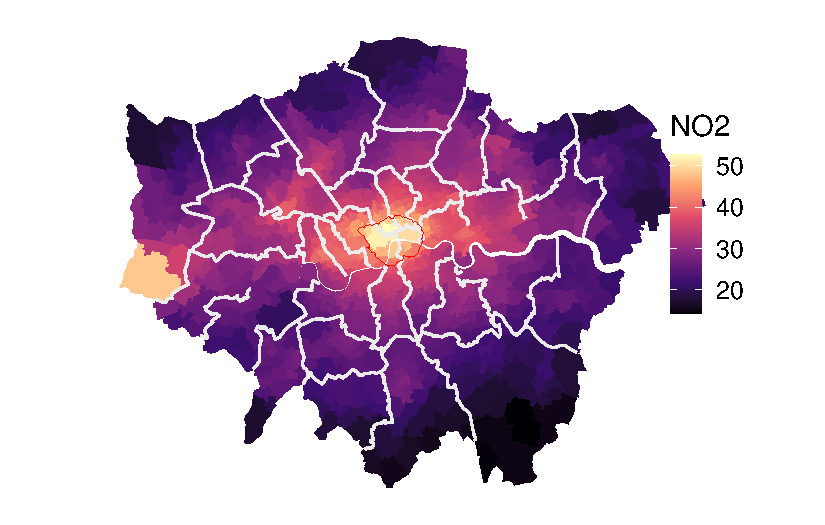
\includegraphics{02_spatial-data_files/figure-pdf/unnamed-chunk-23-1.pdf}

}

\end{figure}

\hypertarget{exercises}{%
\section{Exercises}\label{exercises}}

\begin{enumerate}
\def\labelenumi{\arabic{enumi})}
\tightlist
\item
  What is the difference between a spatial ``sf'' object and a
  conventional ``data.frame''? What's the purpose of the function
  \texttt{st\_drop\_geometry()}?
\end{enumerate}

It's the same. A spatial ``sf'' object just has an additional column
containing the spatial coordinates.

\begin{enumerate}
\def\labelenumi{\arabic{enumi})}
\setcounter{enumi}{1}
\tightlist
\item
  Using msoa.spdf, please create a spatial data frame that contains only
  the MSOA areas that are within the ulez zone.
\end{enumerate}

\begin{Shaded}
\begin{Highlighting}[]
\NormalTok{sub4.spdf }\OtherTok{\textless{}{-}}\NormalTok{ msoa.spdf[ulez.spdf, ]}
\end{Highlighting}
\end{Shaded}

\begin{enumerate}
\def\labelenumi{\arabic{enumi})}
\setcounter{enumi}{2}
\tightlist
\item
  Please create a map for London (or only the msoa-ulez subset) which
  shows the share of Asian residents (or any other ethnic group).
\end{enumerate}

\begin{Shaded}
\begin{Highlighting}[]
\NormalTok{gp }\OtherTok{\textless{}{-}} \FunctionTok{ggplot}\NormalTok{(msoa.spdf)}\SpecialCharTok{+}
    \FunctionTok{geom\_sf}\NormalTok{(}\FunctionTok{aes}\NormalTok{(}\AttributeTok{fill =}\NormalTok{ per\_asian))}\SpecialCharTok{+}
    \FunctionTok{scale\_fill\_viridis\_c}\NormalTok{(}\AttributeTok{option =} \StringTok{"E"}\NormalTok{)}\SpecialCharTok{+}
    \FunctionTok{coord\_sf}\NormalTok{(}\AttributeTok{datum =} \ConstantTok{NA}\NormalTok{)}\SpecialCharTok{+}
    \FunctionTok{theme\_map}\NormalTok{()}\SpecialCharTok{+}
    \FunctionTok{theme}\NormalTok{(}\AttributeTok{legend.position =} \FunctionTok{c}\NormalTok{(.}\DecValTok{9}\NormalTok{, .}\DecValTok{6}\NormalTok{))}
\NormalTok{gp}
\end{Highlighting}
\end{Shaded}

\begin{figure}[H]

{\centering 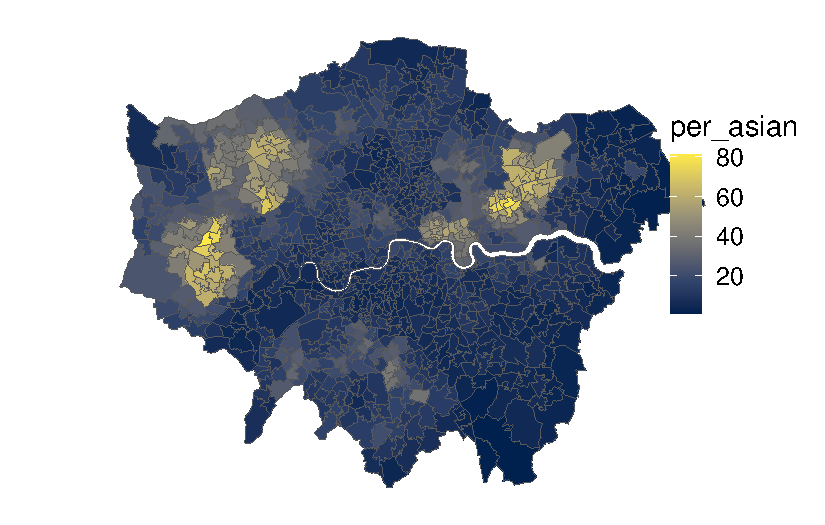
\includegraphics{02_spatial-data_files/figure-pdf/unnamed-chunk-25-1.pdf}

}

\end{figure}

\begin{enumerate}
\def\labelenumi{\arabic{enumi})}
\setcounter{enumi}{3}
\tightlist
\item
  Please calculate the distance of each MSOA to the London city centre
\end{enumerate}

\begin{enumerate}
\def\labelenumi{\alph{enumi})}
\tightlist
\item
  use google maps to get lon and lat,
\item
  use \texttt{st\_as\_sf()} to create the spatial point
\item
  use \texttt{st\_distance()} to calculate the distance
\end{enumerate}

\begin{Shaded}
\begin{Highlighting}[]
\DocumentationTok{\#\#\# Distance to city center}
\CommentTok{\# Define centre}
\NormalTok{centre }\OtherTok{\textless{}{-}} \FunctionTok{st\_as\_sf}\NormalTok{(}\FunctionTok{data.frame}\NormalTok{(}\AttributeTok{lon =} \SpecialCharTok{{-}}\FloatTok{0.128120855701165}\NormalTok{, }
                              \AttributeTok{lat =} \FloatTok{51.50725909644806}\NormalTok{),}
                   \AttributeTok{coords =} \FunctionTok{c}\NormalTok{(}\StringTok{"lon"}\NormalTok{, }\StringTok{"lat"}\NormalTok{), }
                   \AttributeTok{crs =} \DecValTok{4326}\NormalTok{)}
\CommentTok{\# Reproject}
\NormalTok{centre }\OtherTok{\textless{}{-}} \FunctionTok{st\_transform}\NormalTok{(centre, }\AttributeTok{crs =} \FunctionTok{st\_crs}\NormalTok{(msoa.spdf))}
\CommentTok{\# Calculate distance}
\NormalTok{msoa.spdf}\SpecialCharTok{$}\NormalTok{dist\_centre }\OtherTok{\textless{}{-}} \FunctionTok{as.numeric}\NormalTok{(}\FunctionTok{st\_distance}\NormalTok{(msoa.spdf, centre)) }\SpecialCharTok{/} \DecValTok{1000}
\CommentTok{\# hist(msoa.spdf$dist\_centre)}
\end{Highlighting}
\end{Shaded}

\begin{enumerate}
\def\labelenumi{\arabic{enumi})}
\setcounter{enumi}{4}
\tightlist
\item
  Can you create a plot with the distance to the city centre and pub
  counts next to each other?
\end{enumerate}

\begin{Shaded}
\begin{Highlighting}[]
\CommentTok{\# Define colours}
\NormalTok{cols }\OtherTok{\textless{}{-}} \FunctionTok{viridis}\NormalTok{(}\AttributeTok{n =} \DecValTok{10}\NormalTok{, }\AttributeTok{direction =} \DecValTok{1}\NormalTok{, }\AttributeTok{option =} \StringTok{"B"}\NormalTok{)}
\NormalTok{cols2 }\OtherTok{\textless{}{-}} \FunctionTok{viridis}\NormalTok{(}\AttributeTok{n =} \DecValTok{10}\NormalTok{, }\AttributeTok{direction =} \DecValTok{1}\NormalTok{, }\AttributeTok{option =} \StringTok{"E"}\NormalTok{)}


\NormalTok{mp1 }\OtherTok{\textless{}{-}}  \FunctionTok{tm\_shape}\NormalTok{(msoa.spdf) }\SpecialCharTok{+} 
  \FunctionTok{tm\_fill}\NormalTok{(}\AttributeTok{col =} \StringTok{"dist\_centre"}\NormalTok{, }
          \AttributeTok{style =} \StringTok{"fisher"}\NormalTok{, }\CommentTok{\# algorithm to def cut points}
          \AttributeTok{n =} \DecValTok{10}\NormalTok{, }\CommentTok{\# Number of requested cut points}
          \AttributeTok{palette =}\NormalTok{ cols, }\CommentTok{\# colours}
          \AttributeTok{alpha =} \DecValTok{1}\NormalTok{, }\CommentTok{\# transparency }
          \AttributeTok{title =} \StringTok{"Distance"}\NormalTok{, }
          \AttributeTok{legend.hist =} \ConstantTok{FALSE} \CommentTok{\# histogram next to map?}
\NormalTok{          ) }\SpecialCharTok{+}
  \FunctionTok{tm\_borders}\NormalTok{(}\AttributeTok{col =} \StringTok{"white"}\NormalTok{, }\AttributeTok{lwd =} \FloatTok{0.5}\NormalTok{, }\AttributeTok{alpha =} \FloatTok{0.5}\NormalTok{) }\SpecialCharTok{+}
  \FunctionTok{tm\_layout}\NormalTok{(}\AttributeTok{frame =} \ConstantTok{FALSE}\NormalTok{,}
            \AttributeTok{legend.frame =} \ConstantTok{TRUE}\NormalTok{, }\AttributeTok{legend.bg.color =} \ConstantTok{TRUE}\NormalTok{,}
            \AttributeTok{legend.position =} \FunctionTok{c}\NormalTok{(}\StringTok{"right"}\NormalTok{, }\StringTok{"bottom"}\NormalTok{),}
            \AttributeTok{legend.outside =} \ConstantTok{FALSE}\NormalTok{,}
            \AttributeTok{main.title =} \StringTok{"Dist centre"}\NormalTok{, }
            \AttributeTok{main.title.position =} \StringTok{"center"}\NormalTok{,}
            \AttributeTok{main.title.size =} \FloatTok{1.6}\NormalTok{,}
            \AttributeTok{legend.title.size =} \FloatTok{0.8}\NormalTok{,}
            \AttributeTok{legend.text.size =} \FloatTok{0.8}\NormalTok{)}


\NormalTok{mp2 }\OtherTok{\textless{}{-}}  \FunctionTok{tm\_shape}\NormalTok{(msoa.spdf) }\SpecialCharTok{+} 
  \FunctionTok{tm\_fill}\NormalTok{(}\AttributeTok{col =} \StringTok{"dist\_centre"}\NormalTok{, }
          \AttributeTok{style =} \StringTok{"quantile"}\NormalTok{, }\CommentTok{\# algorithm to def cut points}
          \AttributeTok{n =} \DecValTok{10}\NormalTok{, }\CommentTok{\# Number of requested cut points}
          \AttributeTok{palette =}\NormalTok{ cols, }\CommentTok{\# colours}
          \AttributeTok{alpha =} \DecValTok{1}\NormalTok{, }\CommentTok{\# transparency }
          \AttributeTok{title =} \StringTok{"Distance"}\NormalTok{, }
          \AttributeTok{legend.hist =} \ConstantTok{FALSE} \CommentTok{\# histogram next to map?}
\NormalTok{          ) }\SpecialCharTok{+}
  \FunctionTok{tm\_borders}\NormalTok{(}\AttributeTok{col =} \StringTok{"white"}\NormalTok{, }\AttributeTok{lwd =} \FloatTok{0.5}\NormalTok{, }\AttributeTok{alpha =} \FloatTok{0.5}\NormalTok{) }\SpecialCharTok{+}
  \FunctionTok{tm\_layout}\NormalTok{(}\AttributeTok{frame =} \ConstantTok{FALSE}\NormalTok{,}
            \AttributeTok{legend.frame =} \ConstantTok{TRUE}\NormalTok{, }\AttributeTok{legend.bg.color =} \ConstantTok{TRUE}\NormalTok{,}
            \AttributeTok{legend.position =} \FunctionTok{c}\NormalTok{(}\StringTok{"right"}\NormalTok{, }\StringTok{"bottom"}\NormalTok{),}
            \AttributeTok{legend.outside =} \ConstantTok{FALSE}\NormalTok{,}
            \AttributeTok{main.title =} \StringTok{"Dist centre"}\NormalTok{, }
            \AttributeTok{main.title.position =} \StringTok{"center"}\NormalTok{,}
            \AttributeTok{main.title.size =} \FloatTok{1.6}\NormalTok{,}
            \AttributeTok{legend.title.size =} \FloatTok{0.8}\NormalTok{,}
            \AttributeTok{legend.text.size =} \FloatTok{0.8}\NormalTok{)}


\NormalTok{mp3 }\OtherTok{\textless{}{-}}  \FunctionTok{tm\_shape}\NormalTok{(msoa.spdf) }\SpecialCharTok{+} 
  \FunctionTok{tm\_fill}\NormalTok{(}\AttributeTok{col =} \StringTok{"pubs\_count"}\NormalTok{, }
          \AttributeTok{style =} \StringTok{"fisher"}\NormalTok{, }\CommentTok{\# algorithm to def cut points}
          \AttributeTok{n =} \DecValTok{10}\NormalTok{, }\CommentTok{\# Number of requested cut points}
          \AttributeTok{palette =}\NormalTok{ cols, }\CommentTok{\# colours}
          \AttributeTok{alpha =} \DecValTok{1}\NormalTok{, }\CommentTok{\# transparency }
          \AttributeTok{title =} \StringTok{"Count"}\NormalTok{, }
          \AttributeTok{legend.hist =} \ConstantTok{FALSE} \CommentTok{\# histogram next to map?}
\NormalTok{          ) }\SpecialCharTok{+}
  \FunctionTok{tm\_borders}\NormalTok{(}\AttributeTok{col =} \StringTok{"white"}\NormalTok{, }\AttributeTok{lwd =} \FloatTok{0.5}\NormalTok{, }\AttributeTok{alpha =} \FloatTok{0.5}\NormalTok{) }\SpecialCharTok{+}
  \FunctionTok{tm\_layout}\NormalTok{(}\AttributeTok{frame =} \ConstantTok{FALSE}\NormalTok{,}
            \AttributeTok{legend.frame =} \ConstantTok{TRUE}\NormalTok{, }\AttributeTok{legend.bg.color =} \ConstantTok{TRUE}\NormalTok{,}
            \AttributeTok{legend.position =} \FunctionTok{c}\NormalTok{(}\StringTok{"right"}\NormalTok{, }\StringTok{"bottom"}\NormalTok{),}
            \AttributeTok{legend.outside =} \ConstantTok{FALSE}\NormalTok{,}
            \AttributeTok{main.title =} \StringTok{"Pubs"}\NormalTok{, }
            \AttributeTok{main.title.position =} \StringTok{"center"}\NormalTok{,}
            \AttributeTok{main.title.size =} \FloatTok{1.6}\NormalTok{,}
            \AttributeTok{legend.title.size =} \FloatTok{0.8}\NormalTok{,}
            \AttributeTok{legend.text.size =} \FloatTok{0.8}\NormalTok{)}


\NormalTok{mp4 }\OtherTok{\textless{}{-}}  \FunctionTok{tm\_shape}\NormalTok{(msoa.spdf) }\SpecialCharTok{+} 
  \FunctionTok{tm\_fill}\NormalTok{(}\AttributeTok{col =} \StringTok{"pubs\_count"}\NormalTok{, }
          \AttributeTok{style =} \StringTok{"quantile"}\NormalTok{, }\CommentTok{\# algorithm to def cut points}
          \AttributeTok{n =} \DecValTok{10}\NormalTok{, }\CommentTok{\# Number of requested cut points}
          \AttributeTok{palette =}\NormalTok{ cols, }\CommentTok{\# colours}
          \AttributeTok{alpha =} \DecValTok{1}\NormalTok{, }\CommentTok{\# transparency }
          \AttributeTok{title =} \StringTok{"Count"}\NormalTok{, }
          \AttributeTok{legend.hist =} \ConstantTok{FALSE} \CommentTok{\# histogram next to map?}
\NormalTok{          ) }\SpecialCharTok{+}
  \FunctionTok{tm\_borders}\NormalTok{(}\AttributeTok{col =} \StringTok{"white"}\NormalTok{, }\AttributeTok{lwd =} \FloatTok{0.5}\NormalTok{, }\AttributeTok{alpha =} \FloatTok{0.5}\NormalTok{) }\SpecialCharTok{+}
  \FunctionTok{tm\_layout}\NormalTok{(}\AttributeTok{frame =} \ConstantTok{FALSE}\NormalTok{,}
            \AttributeTok{legend.frame =} \ConstantTok{TRUE}\NormalTok{, }\AttributeTok{legend.bg.color =} \ConstantTok{TRUE}\NormalTok{,}
            \AttributeTok{legend.position =} \FunctionTok{c}\NormalTok{(}\StringTok{"right"}\NormalTok{, }\StringTok{"bottom"}\NormalTok{),}
            \AttributeTok{legend.outside =} \ConstantTok{FALSE}\NormalTok{,}
            \AttributeTok{main.title =} \StringTok{"Pubs"}\NormalTok{, }
            \AttributeTok{main.title.position =} \StringTok{"center"}\NormalTok{,}
            \AttributeTok{main.title.size =} \FloatTok{1.6}\NormalTok{,}
            \AttributeTok{legend.title.size =} \FloatTok{0.8}\NormalTok{,}
            \AttributeTok{legend.text.size =} \FloatTok{0.8}\NormalTok{)}


\FunctionTok{tmap\_arrange}\NormalTok{(mp1, mp2, mp3, mp4, }\AttributeTok{ncol =} \DecValTok{2}\NormalTok{, }\AttributeTok{nrow =} \DecValTok{2}\NormalTok{)}
\end{Highlighting}
\end{Shaded}

\begin{figure}[H]

{\centering 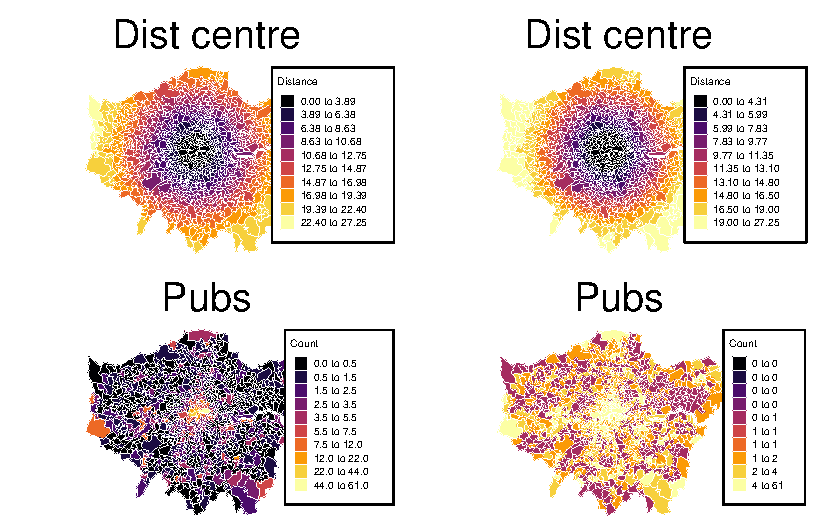
\includegraphics{02_spatial-data_files/figure-pdf/unnamed-chunk-27-1.pdf}

}

\end{figure}

\bookmarksetup{startatroot}

\hypertarget{spatial-relationships-w}{%
\chapter{Spatial Relationships W}\label{spatial-relationships-w}}

\newcommand{\Exp}{\mathrm{E}}
\newcommand\given[1][]{\:#1\vert\:}
\newcommand{\Cov}{\mathrm{Cov}}
\newcommand{\Var}{\mathrm{Var}}
\newcommand{\rank}{\mathrm{rank}}
\newcommand{\bm}[1]{\boldsymbol{\mathbf{#1}}}
\newcommand{\tr}{\mathrm{tr}}
\newcommand{\plim}{\operatornamewithlimits{plim}}
\newcommand{\diag}{\mathrm{diag}}

\hypertarget{required-packages-2}{%
\subsection*{Required packages}\label{required-packages-2}}
\addcontentsline{toc}{subsection}{Required packages}

\begin{Shaded}
\begin{Highlighting}[]
\NormalTok{pkgs }\OtherTok{\textless{}{-}} \FunctionTok{c}\NormalTok{(}\StringTok{"sf"}\NormalTok{, }\StringTok{"mapview"}\NormalTok{, }\StringTok{"spdep"}\NormalTok{, }\StringTok{"spatialreg"}\NormalTok{, }\StringTok{"tmap"}\NormalTok{, }\StringTok{"viridisLite"}\NormalTok{) }\CommentTok{\# note: load spdep first, then spatialreg}
\FunctionTok{lapply}\NormalTok{(pkgs, require, }\AttributeTok{character.only =} \ConstantTok{TRUE}\NormalTok{)}
\end{Highlighting}
\end{Shaded}

\hypertarget{session-info-2}{%
\subsection*{Session info}\label{session-info-2}}
\addcontentsline{toc}{subsection}{Session info}

\begin{Shaded}
\begin{Highlighting}[]
\FunctionTok{sessionInfo}\NormalTok{()}
\end{Highlighting}
\end{Shaded}

\begin{verbatim}
R version 4.4.1 (2024-06-14 ucrt)
Platform: x86_64-w64-mingw32/x64
Running under: Windows 11 x64 (build 22631)

Matrix products: default


locale:
[1] LC_COLLATE=English_United Kingdom.utf8 
[2] LC_CTYPE=English_United Kingdom.utf8   
[3] LC_MONETARY=English_United Kingdom.utf8
[4] LC_NUMERIC=C                           
[5] LC_TIME=English_United Kingdom.utf8    

time zone: Europe/Berlin
tzcode source: internal

attached base packages:
[1] stats     graphics  grDevices utils     datasets  methods   base     

other attached packages:
[1] viridisLite_0.4.2 tmap_3.3-4        spatialreg_1.3-4  Matrix_1.7-0     
[5] spdep_1.3-5       spData_2.3.1      mapview_2.11.2    sf_1.0-16        

loaded via a namespace (and not attached):
 [1] xfun_0.45          raster_3.6-26      htmlwidgets_1.6.4  lattice_0.22-6    
 [5] tools_4.4.1        crosstalk_1.2.1    LearnBayes_2.15.1  parallel_4.4.1    
 [9] stats4_4.4.1       sandwich_3.1-0     proxy_0.4-27       KernSmooth_2.23-24
[13] satellite_1.0.5    RColorBrewer_1.1-3 leaflet_2.2.2      lifecycle_1.0.4   
[17] compiler_4.4.1     deldir_2.0-4       munsell_0.5.1      terra_1.7-78      
[21] codetools_0.2-20   leafsync_0.1.0     stars_0.6-5        htmltools_0.5.8.1 
[25] class_7.3-22       MASS_7.3-60.2      classInt_0.4-10    lwgeom_0.2-14     
[29] wk_0.9.1           abind_1.4-5        boot_1.3-30        multcomp_1.4-25   
[33] nlme_3.1-164       digest_0.6.35      mvtnorm_1.2-5      splines_4.4.1     
[37] fastmap_1.2.0      grid_4.4.1         colorspace_2.1-0   cli_3.6.2         
[41] magrittr_2.0.3     base64enc_0.1-3    dichromat_2.0-0.1  XML_3.99-0.16.1   
[45] survival_3.6-4     leafem_0.2.3       TH.data_1.1-2      e1071_1.7-14      
[49] scales_1.3.0       sp_2.1-4           rmarkdown_2.27     zoo_1.8-12        
[53] png_0.1-8          coda_0.19-4.1      evaluate_0.24.0    knitr_1.47        
[57] tmaptools_3.1-1    s2_1.1.6           rlang_1.1.4        Rcpp_1.0.12       
[61] glue_1.7.0         DBI_1.2.3          rstudioapi_0.16.0  jsonlite_1.8.8    
[65] R6_2.5.1           units_0.8-5       
\end{verbatim}

\hypertarget{reload-data-from-pervious-session-1}{%
\subsection*{Reload data from pervious
session}\label{reload-data-from-pervious-session-1}}
\addcontentsline{toc}{subsection}{Reload data from pervious session}

\begin{Shaded}
\begin{Highlighting}[]
\FunctionTok{load}\NormalTok{(}\StringTok{"\_data/msoa2\_spatial.RData"}\NormalTok{)}
\end{Highlighting}
\end{Shaded}

\hypertarget{spatial-interdependence}{%
\section{Spatial interdependence}\label{spatial-interdependence}}

We can not only use coordinates and geo-spatial information to connect
different data sources, we can also explicitly model spatial
(inter)dependence in the analysis of our data. In many instance,
accounting for spatial dependence might even be necessary to avoid
biased point estimates and standard errors, as observations are often
not independent and identically distributed.

Tobler's first law of geography has been used extensively (11,584
citation in 2023-06) to describe spatial dependence: `Everything is
related to everything else, but near things are more related than
distant things' (Tobler 1970).

\begin{tcolorbox}[enhanced jigsaw, opacitybacktitle=0.6, left=2mm, leftrule=.75mm, toptitle=1mm, breakable, colback=white, bottomrule=.15mm, colframe=quarto-callout-note-color-frame, colbacktitle=quarto-callout-note-color!10!white, coltitle=black, bottomtitle=1mm, titlerule=0mm, title=\textcolor{quarto-callout-note-color}{\faInfo}\hspace{0.5em}{Note}, opacityback=0, arc=.35mm, rightrule=.15mm, toprule=.15mm]

Tobler's first law is a bit of story

And it has been labeled as an excuse to not think too much about the
reasons for spatial dependence or auto-correlation. For instance,
measurement error, omitted variables, or inappropriate levels of
aggregation are among reasons for auto-correlation (Pebesma and Bivand
2023).

\end{tcolorbox}

We will come back to the reasons of spatial dependence. However, for
now, we are interested in some tools to detect and analyse spatial
relations.

To analyse spatial relations, we first need to define some sort of
connectivity between units (e.g.~similar to network analysis). There are
some obvious candidates that be used to define these relations here:
adjacency and proximity.

\hypertarget{boldsymbolmathbfw-connectivity-between-units}{%
\section{\texorpdfstring{\(\boldsymbol{\mathbf{W}}\): Connectivity
between
units}{\textbackslash boldsymbol\{\textbackslash mathbf\{W\}\}: Connectivity between units}}\label{boldsymbolmathbfw-connectivity-between-units}}

The connectivity between units is usually represented in a matrix
\(\boldsymbol{\mathbf{W}}\). There is an ongoing debate about the
importance of spatial weights for spatial econometrics and about the
right way to specify weights matrices (LeSage and Pace 2014; Neumayer
and Plümper 2016). The following graph shows some possible options in
how to define connectivity between units.

\begin{figure}

{\centering \includegraphics{fig/Bivand_neighbours.png}

}

\caption{Figure: Different measures of connectivity, Source: R. S.
Bivand and Rudel (2018)}

\end{figure}

In spatial econometrics, the spatial connectivity (as shown above) is
usually represented by a spatial weights matrix
\({\boldsymbol{\mathbf{W}}}\): \[
\begin{equation} 
        \boldsymbol{\mathbf{W}} = \begin{bmatrix} 
            w_{11} & w_{12} & \dots & w_{1n} \\
            w_{21} & w_{22} & \dots & w_{2n} \\
            \vdots & \vdots & \ddots & \vdots \\
            w_{n1} & w_{n2} & \dots     & w_{nn} 
            \end{bmatrix}
        \end{equation}
\] The spatial weights matrix \(\boldsymbol{\mathbf{W}}\) is an
\(N \times N\) dimensional matrix with elements \(w_{ij}\) specifying
the relation or connectivity between each pair of units \(i\) and \(j\).

Note: The diagonal elements
\(w_{i,i}= w_{1,1}, w_{2,2}, \dots, w_{n,n}\) of
\(\boldsymbol{\mathbf{W}}\) are always zero. No unit is a neighbour of
itself. This is not true for spatial multiplier matrices (as we will see
later).

\hypertarget{contiguity-weights}{%
\subsection{Contiguity weights}\label{contiguity-weights}}

A very common type of spatial weights. Binary specification, taking the
value 1 for neighbouring units (queens: sharing a common edge; rook:
sharing a common border), and 0 otherwise.

Contiguity weights \(w_{i,j}\), where

\begin{equation}
  w_{i,j} =
    \begin{cases}
      1 & \text{if $i$ and $j$ neighbours}\\
      0 & \text{otherwise}
    \end{cases}       
\end{equation}

A contiguity weights matrix with three units, where unit 1 and unit 3
are neighbours, while unit 2 has no neighbours would look like this:

\[
        \begin{equation} 
        \boldsymbol{\mathbf{W}}  = \begin{bmatrix} 
            0 & 0 & 1  \\
            0 & 0 & 0  \\
            1 & 0 & 0  
            \end{bmatrix}   \nonumber
        \end{equation}
\]

\begin{itemize}
\item
  Sparse matrices
\item
  Problem of `island': units without neighbours (if I calculate an
  average of their neigbours, would that be zero, or NA, or a mean?)
\end{itemize}

Lets create a contiguity weights matrix (Queens neighbours) for the
London MSOAs: we create a neighbours list (\texttt{nb}) using
\texttt{poly2nb()}, which is an efficient way of storing
\({\boldsymbol{\mathbf{W}}}\). A \texttt{snap} of 1 meter accounts for
potential lacks of accuracy between lines and points.

\begin{Shaded}
\begin{Highlighting}[]
\CommentTok{\# Contiguity (Queens) neighbours weights}
\NormalTok{queens.nb }\OtherTok{\textless{}{-}} \FunctionTok{poly2nb}\NormalTok{(msoa.spdf, }
                     \AttributeTok{queen =} \ConstantTok{TRUE}\NormalTok{, }\CommentTok{\# a single shared boundary point meets the contiguity condition}
                     \AttributeTok{snap =} \DecValTok{1}\NormalTok{) }\CommentTok{\# we consider points in 1m distance as \textquotesingle{}touching\textquotesingle{}}
\FunctionTok{summary}\NormalTok{(queens.nb)}
\end{Highlighting}
\end{Shaded}

\begin{verbatim}
Neighbour list object:
Number of regions: 983 
Number of nonzero links: 5648 
Percentage nonzero weights: 0.5845042 
Average number of links: 5.745677 
Link number distribution:

  2   3   4   5   6   7   8   9  10  11  12  13 
  9  39 130 264 273 169  66  19   5   6   2   1 
9 least connected regions:
160 270 475 490 597 729 755 778 861 with 2 links
1 most connected region:
946 with 13 links
\end{verbatim}

\begin{Shaded}
\begin{Highlighting}[]
\CommentTok{\# Lets plot that}
\FunctionTok{plot}\NormalTok{(}\FunctionTok{st\_geometry}\NormalTok{(msoa.spdf), }\AttributeTok{border =} \StringTok{"grey60"}\NormalTok{)}
\FunctionTok{plot}\NormalTok{(queens.nb, }\FunctionTok{st\_centroid}\NormalTok{(}\FunctionTok{st\_geometry}\NormalTok{(msoa.spdf)), }
     \AttributeTok{add =} \ConstantTok{TRUE}\NormalTok{, }\AttributeTok{pch =} \DecValTok{19}\NormalTok{, }\AttributeTok{cex =} \FloatTok{0.6}\NormalTok{)}
\end{Highlighting}
\end{Shaded}

\begin{figure}[H]

{\centering 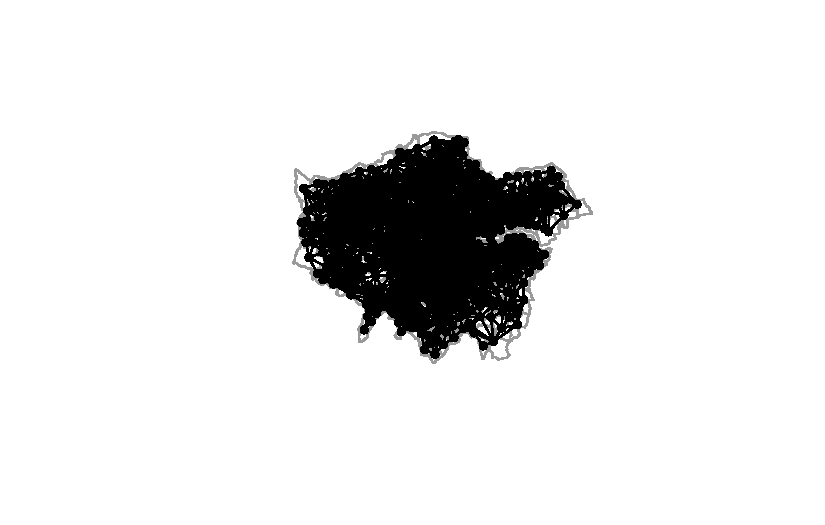
\includegraphics{03_weights_files/figure-pdf/unnamed-chunk-4-1.pdf}

}

\end{figure}

\begin{Shaded}
\begin{Highlighting}[]
\CommentTok{\# We can also transform this into a matrix W}
\NormalTok{W }\OtherTok{\textless{}{-}} \FunctionTok{nb2mat}\NormalTok{(queens.nb, }\AttributeTok{style =} \StringTok{"B"}\NormalTok{)}
\FunctionTok{print}\NormalTok{(W[}\DecValTok{1}\SpecialCharTok{:}\DecValTok{10}\NormalTok{, }\DecValTok{1}\SpecialCharTok{:}\DecValTok{10}\NormalTok{])}
\end{Highlighting}
\end{Shaded}

\begin{verbatim}
   [,1] [,2] [,3] [,4] [,5] [,6] [,7] [,8] [,9] [,10]
1     0    0    0    0    0    0    0    0    0     0
2     0    0    1    0    0    0    0    0    0     0
3     0    1    0    0    1    0    0    0    0     0
4     0    0    0    0    0    1    0    0    0     1
5     0    0    1    0    0    1    1    0    0     0
6     0    0    0    1    1    0    1    0    1     1
7     0    0    0    0    1    1    0    1    1     0
8     0    0    0    0    0    0    1    0    0     0
9     0    0    0    0    0    1    1    0    0     1
10    0    0    0    1    0    1    0    0    1     0
\end{verbatim}

\begin{tcolorbox}[enhanced jigsaw, opacitybacktitle=0.6, left=2mm, leftrule=.75mm, toptitle=1mm, breakable, colback=white, bottomrule=.15mm, colframe=quarto-callout-tip-color-frame, colbacktitle=quarto-callout-tip-color!10!white, coltitle=black, bottomtitle=1mm, titlerule=0mm, title=\textcolor{quarto-callout-tip-color}{\faLightbulb}\hspace{0.5em}{Question}, opacityback=0, arc=.35mm, rightrule=.15mm, toprule=.15mm]

Among those first 10 units that you see above, which are the neighbours
of unit number 6?

Why is the diagonal of this matrix all zero?

\end{tcolorbox}

Overall, the matrix W has dimensions \(N \times N\), a row and a column
for each observation. The value in a cell shows how units \(i\) (row
number) and \(j\) (column number) are related to each other.

\begin{Shaded}
\begin{Highlighting}[]
\FunctionTok{dim}\NormalTok{(W)}
\end{Highlighting}
\end{Shaded}

\begin{verbatim}
[1] 983 983
\end{verbatim}

The row and column sums indicate the number of neighbours of each
observation.

\begin{Shaded}
\begin{Highlighting}[]
\FunctionTok{rowSums}\NormalTok{(W)[}\DecValTok{1}\SpecialCharTok{:}\DecValTok{10}\NormalTok{]}
\end{Highlighting}
\end{Shaded}

\begin{verbatim}
 1  2  3  4  5  6  7  8  9 10 
11  6  7  5  5  6  6  6  6  5 
\end{verbatim}

\begin{Shaded}
\begin{Highlighting}[]
\FunctionTok{colSums}\NormalTok{(W)[}\DecValTok{1}\SpecialCharTok{:}\DecValTok{10}\NormalTok{]}
\end{Highlighting}
\end{Shaded}

\begin{verbatim}
 [1] 11  6  7  5  5  6  6  6  6  5
\end{verbatim}

Adjacency or graph-based neighbour's weights matrices are usually
symmetric. If unit 1 is a neighbour of unit 55, then unit 55 is also a
neighbour of unit 1.

\begin{tcolorbox}[enhanced jigsaw, opacitybacktitle=0.6, left=2mm, leftrule=.75mm, toptitle=1mm, breakable, colback=white, bottomrule=.15mm, colframe=quarto-callout-tip-color-frame, colbacktitle=quarto-callout-tip-color!10!white, coltitle=black, bottomtitle=1mm, titlerule=0mm, title=\textcolor{quarto-callout-tip-color}{\faLightbulb}\hspace{0.5em}{Higher Order Neighbours}, opacityback=0, arc=.35mm, rightrule=.15mm, toprule=.15mm]

Your neighbours have neighbours too, and they are called higher (second)
order neighbours. The neighbours of your neighbour's neighbours are
third order neighbours.

You can use \texttt{nblag()} to calculate higher order neighbour
relations.

\end{tcolorbox}

\hypertarget{distance-based-weights}{%
\subsection{Distance based weights}\label{distance-based-weights}}

Another common type uses the distance \(d_{ij}\) between each unit \(i\)
and \(j\).

\begin{itemize}
\tightlist
\item
  Inverse distance weights \(w_{i,j} = \frac{1}{d_{ij}^\alpha}\), where
  \(\alpha\) define the strength of the spatial decay.
\end{itemize}

\[
        \begin{equation} 
        \boldsymbol{\mathbf{W}} = \begin{bmatrix} 
            0 & \frac{1}{d_{ij}^\alpha} & \frac{1}{d_{ij}^\alpha}  \\
            \frac{1}{d_{ij}^\alpha} & 0 & \frac{1}{d_{ij}^\alpha}  \\
            \frac{1}{d_{ij}^\alpha} & \frac{1}{d_{ij}^\alpha} & 0  
            \end{bmatrix}   \nonumber
        \end{equation}
\]

\begin{itemize}
\item
  Dense matrices
\item
  Specifying thresholds may be useful (to get rid of very small non-zero
  weights)
\end{itemize}

For now, we will just specify a neighbours list with a distance
threshold of 3km using \texttt{dnearneigh()}. An alternative would be k
nearest neighbours using \texttt{knearneigh()}. We will do the inverse
weighting later.

\begin{Shaded}
\begin{Highlighting}[]
\CommentTok{\# Crease centroids}
\NormalTok{coords }\OtherTok{\textless{}{-}} \FunctionTok{st\_geometry}\NormalTok{(}\FunctionTok{st\_centroid}\NormalTok{(msoa.spdf))}
\end{Highlighting}
\end{Shaded}

\begin{verbatim}
Warning: st_centroid assumes attributes are constant over geometries
\end{verbatim}

\begin{Shaded}
\begin{Highlighting}[]
\CommentTok{\# Neighbours within 3km distance}
\NormalTok{dist\_3.nb }\OtherTok{\textless{}{-}} \FunctionTok{dnearneigh}\NormalTok{(coords, }\AttributeTok{d1 =} \DecValTok{0}\NormalTok{, }\AttributeTok{d2 =} \DecValTok{3000}\NormalTok{)}
\FunctionTok{summary}\NormalTok{(dist\_3.nb)}
\end{Highlighting}
\end{Shaded}

\begin{verbatim}
Neighbour list object:
Number of regions: 983 
Number of nonzero links: 22086 
Percentage nonzero weights: 2.285652 
Average number of links: 22.46796 
2 disjoint connected subgraphs
Link number distribution:

 1  2  3  4  5  6  7  8  9 10 11 12 13 14 15 16 17 18 19 20 21 22 23 24 25 26 
 4  3  7 13 11 14 14 17 26 22 26 30 33 34 46 34 59 43 38 30 25 19 22 15 21 14 
27 28 29 30 31 32 33 34 35 36 37 38 39 40 41 42 43 44 45 46 47 
23 17 17 23 28 19 26 24 29 24 27 25 22 18  8 10 12  5  3  2  1 
4 least connected regions:
158 160 463 959 with 1 link
1 most connected region:
545 with 47 links
\end{verbatim}

\begin{Shaded}
\begin{Highlighting}[]
\CommentTok{\# Lets plot that}
\FunctionTok{plot}\NormalTok{(}\FunctionTok{st\_geometry}\NormalTok{(msoa.spdf), }\AttributeTok{border =} \StringTok{"grey60"}\NormalTok{)}
\FunctionTok{plot}\NormalTok{(dist\_3.nb, coords, }
     \AttributeTok{add =} \ConstantTok{TRUE}\NormalTok{, }\AttributeTok{pch =} \DecValTok{19}\NormalTok{, }\AttributeTok{cex =} \FloatTok{0.6}\NormalTok{)}
\end{Highlighting}
\end{Shaded}

\begin{figure}[H]

{\centering 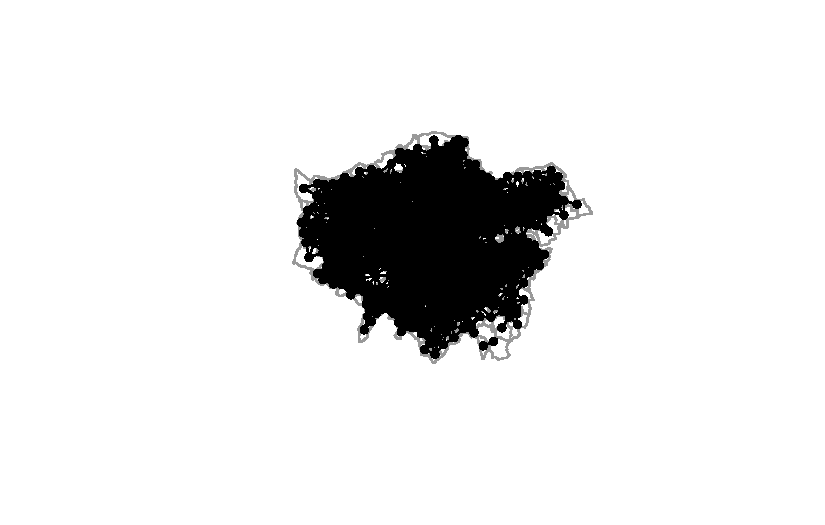
\includegraphics{03_weights_files/figure-pdf/unnamed-chunk-7-1.pdf}

}

\end{figure}

And you can see that the matrix is not so sparse anymore:

\begin{Shaded}
\begin{Highlighting}[]
\NormalTok{W2 }\OtherTok{\textless{}{-}} \FunctionTok{nb2mat}\NormalTok{(dist\_3.nb, }\AttributeTok{style =} \StringTok{"B"}\NormalTok{)}
\NormalTok{W2[}\DecValTok{1}\SpecialCharTok{:}\DecValTok{10}\NormalTok{, }\DecValTok{1}\SpecialCharTok{:}\DecValTok{10}\NormalTok{]}
\end{Highlighting}
\end{Shaded}

\begin{verbatim}
   [,1] [,2] [,3] [,4] [,5] [,6] [,7] [,8] [,9] [,10]
1     0    0    0    0    0    0    0    0    0     0
2     0    0    1    0    1    0    0    0    0     0
3     0    1    0    0    1    1    1    0    0     0
4     0    0    0    0    1    1    1    0    1     1
5     0    1    1    1    0    1    1    1    1     1
6     0    0    1    1    1    0    1    1    1     1
7     0    0    1    1    1    1    0    1    1     1
8     0    0    0    0    1    1    1    0    1     0
9     0    0    0    1    1    1    1    1    0     1
10    0    0    0    1    1    1    1    0    1     0
\end{verbatim}

\hypertarget{normalization-of-boldsymbolmathbfw}{%
\section{\texorpdfstring{Normalization of
\({\boldsymbol{\mathbf{W}}}\)}{Normalization of \{\textbackslash boldsymbol\{\textbackslash mathbf\{W\}\}\}}}\label{normalization-of-boldsymbolmathbfw}}

Normalizing ensures that the parameter space of the spatial multiplier
is restricted to \(-1 < \rho > 1\), and the multiplier matrix is
non-singular (don't worry, more on this later).

The main message: Normalizing your weights matrix is always a good idea.
Otherwise, the spatial parameters might blow up -- if you can estimate
the model at all. It also ensure easy interpretation of spillover
effects.

Again, how to normalize a weights matrix is subject of debate (LeSage
and Pace 2014; Neumayer and Plümper 2016).

\hypertarget{row-normalization}{%
\subsection{Row-normalization}\label{row-normalization}}

Row-normalization divides each non-zero weight by the sum of all weights
of unit \(i\), which is the sum of the row.

\[
\frac{w_{ij}}{\sum_j^n w_{ij}}
\]

\begin{itemize}
\item
  With contiguity weights, spatially lagged variables contain mean of
  this variable among the neighbours of \(i\)
\item
  Proportions between units such as distances get lost (can be bad!)
\item
  Can induce asymmetries: \(w_{ij} \neq w_{ji}\)
\end{itemize}

For instance, we can use row-normalization for the Queens neighbours
created above, and create a neighbours list with spatial weights.

\begin{Shaded}
\begin{Highlighting}[]
\NormalTok{queens.lw }\OtherTok{\textless{}{-}} \FunctionTok{nb2listw}\NormalTok{(queens.nb,}
                      \AttributeTok{style =} \StringTok{"W"}\NormalTok{) }\CommentTok{\# W ist row{-}normalization}
\FunctionTok{summary}\NormalTok{(queens.lw)}
\end{Highlighting}
\end{Shaded}

\begin{verbatim}
Characteristics of weights list object:
Neighbour list object:
Number of regions: 983 
Number of nonzero links: 5648 
Percentage nonzero weights: 0.5845042 
Average number of links: 5.745677 
Link number distribution:

  2   3   4   5   6   7   8   9  10  11  12  13 
  9  39 130 264 273 169  66  19   5   6   2   1 
9 least connected regions:
160 270 475 490 597 729 755 778 861 with 2 links
1 most connected region:
946 with 13 links

Weights style: W 
Weights constants summary:
    n     nn  S0       S1      S2
W 983 966289 983 355.1333 4017.47
\end{verbatim}

To see what happened, let's look at our example in matrix format again.

\begin{Shaded}
\begin{Highlighting}[]
\CommentTok{\# transform into matrix with row{-}normalization}
\NormalTok{W\_norm }\OtherTok{\textless{}{-}} \FunctionTok{nb2mat}\NormalTok{(queens.nb, }\AttributeTok{style =} \StringTok{"W"}\NormalTok{)}
\FunctionTok{print}\NormalTok{(W\_norm[}\DecValTok{1}\SpecialCharTok{:}\DecValTok{10}\NormalTok{, }\DecValTok{1}\SpecialCharTok{:}\DecValTok{10}\NormalTok{])}
\end{Highlighting}
\end{Shaded}

\begin{verbatim}
   [,1]      [,2]      [,3]      [,4]      [,5]      [,6]      [,7]      [,8]
1     0 0.0000000 0.0000000 0.0000000 0.0000000 0.0000000 0.0000000 0.0000000
2     0 0.0000000 0.1666667 0.0000000 0.0000000 0.0000000 0.0000000 0.0000000
3     0 0.1428571 0.0000000 0.0000000 0.1428571 0.0000000 0.0000000 0.0000000
4     0 0.0000000 0.0000000 0.0000000 0.0000000 0.2000000 0.0000000 0.0000000
5     0 0.0000000 0.2000000 0.0000000 0.0000000 0.2000000 0.2000000 0.0000000
6     0 0.0000000 0.0000000 0.1666667 0.1666667 0.0000000 0.1666667 0.0000000
7     0 0.0000000 0.0000000 0.0000000 0.1666667 0.1666667 0.0000000 0.1666667
8     0 0.0000000 0.0000000 0.0000000 0.0000000 0.0000000 0.1666667 0.0000000
9     0 0.0000000 0.0000000 0.0000000 0.0000000 0.1666667 0.1666667 0.0000000
10    0 0.0000000 0.0000000 0.2000000 0.0000000 0.2000000 0.0000000 0.0000000
        [,9]     [,10]
1  0.0000000 0.0000000
2  0.0000000 0.0000000
3  0.0000000 0.0000000
4  0.0000000 0.2000000
5  0.0000000 0.0000000
6  0.1666667 0.1666667
7  0.1666667 0.0000000
8  0.0000000 0.0000000
9  0.0000000 0.1666667
10 0.2000000 0.0000000
\end{verbatim}

\begin{tcolorbox}[enhanced jigsaw, opacitybacktitle=0.6, left=2mm, leftrule=.75mm, toptitle=1mm, breakable, colback=white, bottomrule=.15mm, colframe=quarto-callout-tip-color-frame, colbacktitle=quarto-callout-tip-color!10!white, coltitle=black, bottomtitle=1mm, titlerule=0mm, title=\textcolor{quarto-callout-tip-color}{\faLightbulb}\hspace{0.5em}{Question}, opacityback=0, arc=.35mm, rightrule=.15mm, toprule=.15mm]

Overall, how many neighbours does unit 9 have (including all columns)?
How do you know?

\end{tcolorbox}

\begin{Shaded}
\begin{Highlighting}[]
\FunctionTok{rowSums}\NormalTok{(W)[}\DecValTok{9}\NormalTok{]}
\end{Highlighting}
\end{Shaded}

We can also use the nb object to see which ones the neighbours are.
Here, for instance, neighbours of unit 6:

\begin{Shaded}
\begin{Highlighting}[]
\NormalTok{queens.nb[}\DecValTok{6}\NormalTok{]}
\end{Highlighting}
\end{Shaded}

\begin{verbatim}
[[1]]
[1]   4   5   7   9  10 462
\end{verbatim}

This fits to what we see in the matrix above.

\begin{tcolorbox}[enhanced jigsaw, opacitybacktitle=0.6, left=2mm, leftrule=.75mm, toptitle=1mm, breakable, colback=white, bottomrule=.15mm, colframe=quarto-callout-warning-color-frame, colbacktitle=quarto-callout-warning-color!10!white, coltitle=black, bottomtitle=1mm, titlerule=0mm, title=\textcolor{quarto-callout-warning-color}{\faExclamationTriangle}\hspace{0.5em}{Warning}, opacityback=0, arc=.35mm, rightrule=.15mm, toprule=.15mm]

Note that row-normalization has some undesirable properties when we use
some non-contigutiy based neighbour relations, such as distance based
neighbours.

The problem: It obscures the proportion due to dividing by a
row-specific value.

\end{tcolorbox}

Let's construct a hypothetical example

\begin{Shaded}
\begin{Highlighting}[]
\CommentTok{\# Subset of 5 units}
\NormalTok{sub.spdf }\OtherTok{\textless{}{-}}\NormalTok{ msoa.spdf[}\FunctionTok{c}\NormalTok{(}\DecValTok{4}\NormalTok{, }\DecValTok{5}\NormalTok{, }\DecValTok{6}\NormalTok{, }\DecValTok{102}\NormalTok{, }\DecValTok{150}\NormalTok{), ]}
\FunctionTok{mapview}\NormalTok{(sub.spdf)}
\end{Highlighting}
\end{Shaded}

\begin{figure}[H]

{\centering 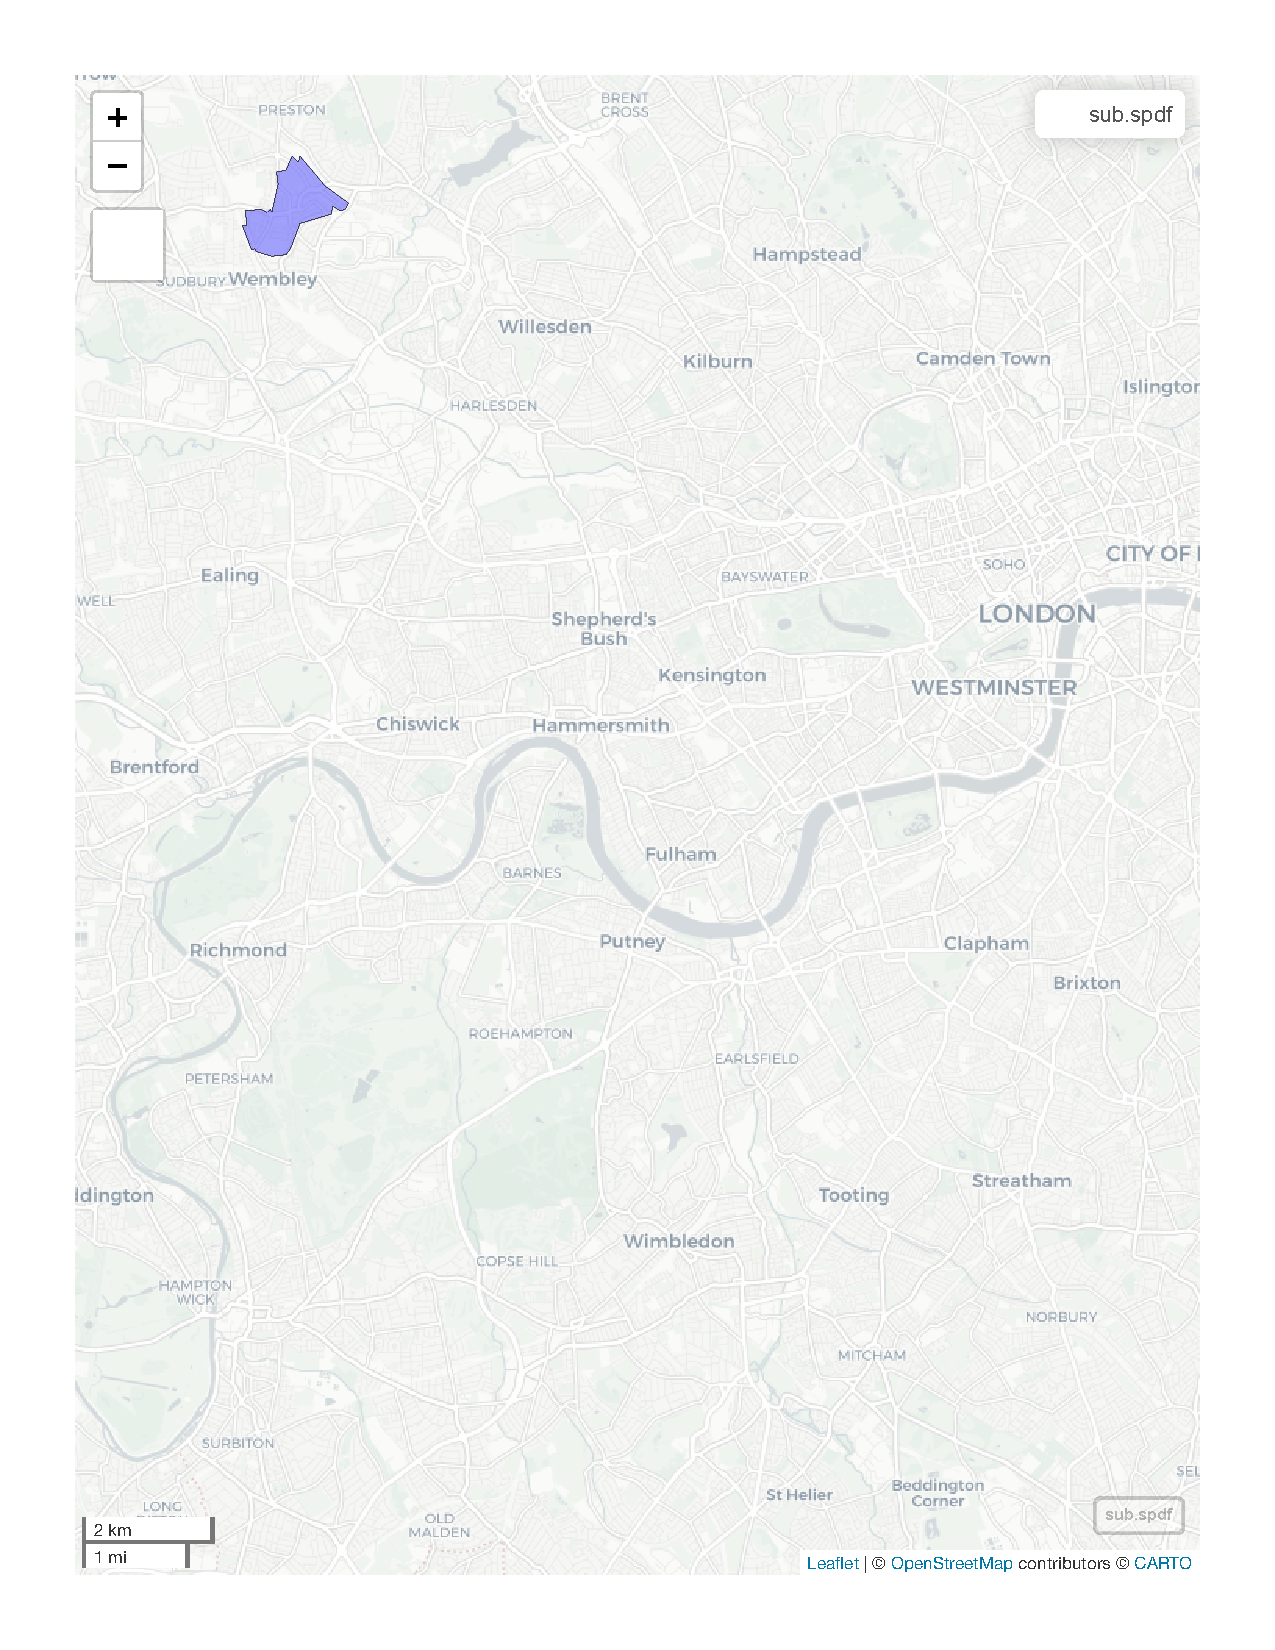
\includegraphics{03_weights_files/figure-pdf/unnamed-chunk-13-1.pdf}

}

\end{figure}

We construct the \textbf{inverse-distance weighted 2 nearest neighbors}.

\begin{Shaded}
\begin{Highlighting}[]
\CommentTok{\# 2 closest neighbours}
\NormalTok{sub.coords }\OtherTok{\textless{}{-}} \FunctionTok{st\_geometry}\NormalTok{(}\FunctionTok{st\_centroid}\NormalTok{(sub.spdf))}
\end{Highlighting}
\end{Shaded}

\begin{verbatim}
Warning: st_centroid assumes attributes are constant over geometries
\end{verbatim}

\begin{Shaded}
\begin{Highlighting}[]
\NormalTok{knn.nb }\OtherTok{\textless{}{-}} \FunctionTok{knearneigh}\NormalTok{(sub.coords, }
                     \AttributeTok{k =} \DecValTok{2}\NormalTok{) }\CommentTok{\# number of nearest neighbours}
\end{Highlighting}
\end{Shaded}

\begin{verbatim}
Warning in knearneigh(sub.coords, k = 2): k greater than one-third of the
number of data points
\end{verbatim}

\begin{Shaded}
\begin{Highlighting}[]
\NormalTok{knn.nb }\OtherTok{\textless{}{-}} \FunctionTok{knn2nb}\NormalTok{(knn.nb)}
\FunctionTok{summary}\NormalTok{(knn.nb)}
\end{Highlighting}
\end{Shaded}

\begin{verbatim}
Neighbour list object:
Number of regions: 5 
Number of nonzero links: 10 
Percentage nonzero weights: 40 
Average number of links: 2 
Non-symmetric neighbours list
Link number distribution:

2 
5 
5 least connected regions:
1 2 3 4 5 with 2 links
5 most connected regions:
1 2 3 4 5 with 2 links
\end{verbatim}

\begin{Shaded}
\begin{Highlighting}[]
\CommentTok{\# listw with inverse{-}distance based weights}
\NormalTok{sub.lw }\OtherTok{\textless{}{-}} \FunctionTok{nb2listwdist}\NormalTok{(knn.nb,}
                       \AttributeTok{x =}\NormalTok{ sub.coords, }\CommentTok{\# needed for idw}
                       \AttributeTok{type =} \StringTok{"idw"}\NormalTok{, }\CommentTok{\# inverse distance weighting}
                       \AttributeTok{alpha =} \DecValTok{1}\NormalTok{, }\CommentTok{\# the decay parameter for distance weighting}
                       \AttributeTok{style =} \StringTok{"raw"}\NormalTok{) }\CommentTok{\# without normalization}
\NormalTok{W\_sub }\OtherTok{\textless{}{-}} \FunctionTok{listw2mat}\NormalTok{(sub.lw)}
\FunctionTok{formatC}\NormalTok{(W\_sub, }\AttributeTok{format =} \StringTok{"f"}\NormalTok{, }\AttributeTok{digits =} \DecValTok{6}\NormalTok{)}
\end{Highlighting}
\end{Shaded}

\begin{verbatim}
  [,1]       [,2]       [,3]       [,4]       [,5]      
1 "0.000000" "0.000414" "0.000723" "0.000000" "0.000000"
2 "0.000414" "0.000000" "0.000962" "0.000000" "0.000000"
3 "0.000723" "0.000962" "0.000000" "0.000000" "0.000000"
4 "0.000000" "0.000033" "0.000032" "0.000000" "0.000000"
5 "0.000049" "0.000000" "0.000049" "0.000000" "0.000000"
\end{verbatim}

As you can see, units 1, 2, 3 have relatively proximate neighbours (.e.g
inverse distance 0.000962: 3 zeros). Units 4 and 5, in contrast, have
only very distant neighbours (e.g.~inverse distance 0.000049: 4 zeros).

Now, see what happens when we use row-normalization.

\begin{Shaded}
\begin{Highlighting}[]
\NormalTok{sub.lw }\OtherTok{\textless{}{-}} \FunctionTok{nb2listwdist}\NormalTok{(knn.nb,}
                       \AttributeTok{x =}\NormalTok{ sub.coords, }\CommentTok{\# needed for idw}
                       \AttributeTok{type =} \StringTok{"idw"}\NormalTok{, }\CommentTok{\# inverse distance weighting}
                       \AttributeTok{alpha =} \DecValTok{1}\NormalTok{, }\CommentTok{\# the decay parameter for distance weighting}
                       \AttributeTok{style =} \StringTok{"W"}\NormalTok{) }\CommentTok{\# for row normalization}
\NormalTok{W\_sub }\OtherTok{\textless{}{-}} \FunctionTok{listw2mat}\NormalTok{(sub.lw)}
\FunctionTok{formatC}\NormalTok{(W\_sub, }\AttributeTok{format =} \StringTok{"f"}\NormalTok{, }\AttributeTok{digits =} \DecValTok{6}\NormalTok{)}
\end{Highlighting}
\end{Shaded}

\begin{verbatim}
  [,1]       [,2]       [,3]       [,4]       [,5]      
1 "0.000000" "0.364083" "0.635917" "0.000000" "0.000000"
2 "0.300879" "0.000000" "0.699121" "0.000000" "0.000000"
3 "0.429123" "0.570877" "0.000000" "0.000000" "0.000000"
4 "0.000000" "0.507955" "0.492045" "0.000000" "0.000000"
5 "0.499360" "0.000000" "0.500640" "0.000000" "0.000000"
\end{verbatim}

All rows sum up to 1, but the strength of the relation is now similar
for the distant units 4 and 5, and the proximate units 1, 2, 3.

\hypertarget{maximum-eigenvalues-normalization}{%
\subsection{Maximum eigenvalues
normalization}\label{maximum-eigenvalues-normalization}}

Maximum eigenvalues normalization divides each non-zero weight by the
overall maximum eigenvalue \(\lambda_{max}\). Each element of
\(\boldsymbol{\mathbf{W}}\) is divided by the same scalar parameter,
which preserves the relations.

\[
\frac{\boldsymbol{\mathbf{W}}}{\lambda_{max}}
\]

\begin{itemize}
\item
  Interpretation may become more complicated
\item
  Keeps proportions of connectivity strengths across units (relevant
  esp.~for distance based \(\boldsymbol{\mathbf{W}}\))
\end{itemize}

We use eigenvalue normalization for the inverse distance neighbours. We
use \texttt{nb2listwdist()} to create weight inverse distance based
weights and normalize in one step.

\begin{Shaded}
\begin{Highlighting}[]
\NormalTok{coords }\OtherTok{\textless{}{-}} \FunctionTok{st\_geometry}\NormalTok{(}\FunctionTok{st\_centroid}\NormalTok{(msoa.spdf))}
\end{Highlighting}
\end{Shaded}

\begin{verbatim}
Warning: st_centroid assumes attributes are constant over geometries
\end{verbatim}

\begin{Shaded}
\begin{Highlighting}[]
\NormalTok{idw.lw }\OtherTok{\textless{}{-}} \FunctionTok{nb2listwdist}\NormalTok{(dist\_3.nb,}
                       \AttributeTok{x =}\NormalTok{ coords, }\CommentTok{\# needed for idw}
                       \AttributeTok{type =} \StringTok{"idw"}\NormalTok{, }\CommentTok{\# inverse distance weighting}
                       \AttributeTok{alpha =} \DecValTok{1}\NormalTok{, }\CommentTok{\# the decay parameter for distance weighting}
                       \AttributeTok{style =} \StringTok{"minmax"}\NormalTok{) }\CommentTok{\# for eigenvalue normalization}
\FunctionTok{summary}\NormalTok{(idw.lw)}
\end{Highlighting}
\end{Shaded}

\begin{verbatim}
Characteristics of weights list object:
Neighbour list object:
Number of regions: 983 
Number of nonzero links: 22086 
Percentage nonzero weights: 2.285652 
Average number of links: 22.46796 
2 disjoint connected subgraphs
Link number distribution:

 1  2  3  4  5  6  7  8  9 10 11 12 13 14 15 16 17 18 19 20 21 22 23 24 25 26 
 4  3  7 13 11 14 14 17 26 22 26 30 33 34 46 34 59 43 38 30 25 19 22 15 21 14 
27 28 29 30 31 32 33 34 35 36 37 38 39 40 41 42 43 44 45 46 47 
23 17 17 23 28 19 26 24 29 24 27 25 22 18  8 10 12  5  3  2  1 
4 least connected regions:
158 160 463 959 with 1 link
1 most connected region:
545 with 47 links

Weights style: minmax 
Weights constants summary:
         n     nn       S0       S1       S2
minmax 983 966289 463.6269 23.92505 1117.636
\end{verbatim}

Examples from above: See how this keeps the proportions in our example.
Instead of transforming values to sum up to 1 in each row, we now have
much smaller values for 4 and 5 then we have for the proximate units 1,
2, 3.

\begin{Shaded}
\begin{Highlighting}[]
\NormalTok{sub.lw }\OtherTok{\textless{}{-}} \FunctionTok{nb2listwdist}\NormalTok{(knn.nb,}
                       \AttributeTok{x =}\NormalTok{ sub.coords, }\CommentTok{\# needed for idw}
                       \AttributeTok{type =} \StringTok{"idw"}\NormalTok{, }\CommentTok{\# inverse distance weighting}
                       \AttributeTok{alpha =} \DecValTok{1}\NormalTok{, }\CommentTok{\# the decay parameter for distance weighting}
                       \AttributeTok{style =} \StringTok{"minmax"}\NormalTok{) }\CommentTok{\# for eigenvalue normalization}
\NormalTok{W\_sub }\OtherTok{\textless{}{-}} \FunctionTok{listw2mat}\NormalTok{(sub.lw)}
\FunctionTok{formatC}\NormalTok{(W\_sub, }\AttributeTok{format =} \StringTok{"f"}\NormalTok{, }\AttributeTok{digits =} \DecValTok{6}\NormalTok{)}
\end{Highlighting}
\end{Shaded}

\begin{verbatim}
  [,1]       [,2]       [,3]       [,4]       [,5]      
1 "0.000000" "0.245687" "0.429123" "0.000000" "0.000000"
2 "0.245687" "0.000000" "0.570877" "0.000000" "0.000000"
3 "0.429123" "0.570877" "0.000000" "0.000000" "0.000000"
4 "0.000000" "0.019663" "0.019047" "0.000000" "0.000000"
5 "0.029099" "0.000000" "0.029174" "0.000000" "0.000000"
\end{verbatim}

\hypertarget{islands-missings}{%
\section{Islands / missings}\label{islands-missings}}

In practice, we often have a problem with islands. If we use contiguity
based or distance based neighbour definitions, some units may end up
with empty neighbours sets: they just do not touch any other unit and do
not have a neighbour within a specific distance. This however creates a
problem: what is the value in the neighbouring units?

The \texttt{zero.policy} option in \texttt{spdep} allows to proceed with
empty neighbours sets. However, many further functions may run into
problems and return errors. It often makes sense to either drop islands,
to choose weights which always have neighbours (e.g.~k nearest), or
impute empty neighbours sets by using the nearest neighbours.

\bookmarksetup{startatroot}

\hypertarget{exercises-i}{%
\chapter{Exercises I}\label{exercises-i}}

\hypertarget{required-packages-3}{%
\subsection*{Required packages}\label{required-packages-3}}
\addcontentsline{toc}{subsection}{Required packages}

\begin{Shaded}
\begin{Highlighting}[]
\NormalTok{pkgs }\OtherTok{\textless{}{-}} \FunctionTok{c}\NormalTok{(}\StringTok{"sf"}\NormalTok{, }\StringTok{"mapview"}\NormalTok{, }\StringTok{"spdep"}\NormalTok{, }\StringTok{"spatialreg"}\NormalTok{, }\StringTok{"tmap"}\NormalTok{, }\StringTok{"viridisLite"}\NormalTok{,}
          \StringTok{"ggplot2"}\NormalTok{, }\StringTok{"ggthemes"}\NormalTok{) }\CommentTok{\# note: load spdep first, then spatialreg}
\FunctionTok{lapply}\NormalTok{(pkgs, require, }\AttributeTok{character.only =} \ConstantTok{TRUE}\NormalTok{)}
\end{Highlighting}
\end{Shaded}

\hypertarget{session-info-3}{%
\subsection*{Session info}\label{session-info-3}}
\addcontentsline{toc}{subsection}{Session info}

\begin{Shaded}
\begin{Highlighting}[]
\FunctionTok{sessionInfo}\NormalTok{()}
\end{Highlighting}
\end{Shaded}

\begin{verbatim}
R version 4.4.1 (2024-06-14 ucrt)
Platform: x86_64-w64-mingw32/x64
Running under: Windows 11 x64 (build 22631)

Matrix products: default


locale:
[1] LC_COLLATE=English_United Kingdom.utf8 
[2] LC_CTYPE=English_United Kingdom.utf8   
[3] LC_MONETARY=English_United Kingdom.utf8
[4] LC_NUMERIC=C                           
[5] LC_TIME=English_United Kingdom.utf8    

time zone: Europe/Berlin
tzcode source: internal

attached base packages:
[1] stats     graphics  grDevices utils     datasets  methods   base     

other attached packages:
 [1] ggthemes_5.1.0    ggplot2_3.5.1     viridisLite_0.4.2 tmap_3.3-4       
 [5] spatialreg_1.3-4  Matrix_1.7-0      spdep_1.3-5       spData_2.3.1     
 [9] mapview_2.11.2    sf_1.0-16        

loaded via a namespace (and not attached):
 [1] tidyselect_1.2.1   dplyr_1.1.4        fastmap_1.2.0      leaflet_2.2.2     
 [5] TH.data_1.1-2      XML_3.99-0.16.1    digest_0.6.35      lifecycle_1.0.4   
 [9] LearnBayes_2.15.1  survival_3.6-4     terra_1.7-78       magrittr_2.0.3    
[13] compiler_4.4.1     rlang_1.1.4        tools_4.4.1        utf8_1.2.4        
[17] knitr_1.47         htmlwidgets_1.6.4  sp_2.1-4           classInt_0.4-10   
[21] RColorBrewer_1.1-3 multcomp_1.4-25    abind_1.4-5        KernSmooth_2.23-24
[25] purrr_1.0.2        withr_3.0.0        leafsync_0.1.0     grid_4.4.1        
[29] stats4_4.4.1       fansi_1.0.6        e1071_1.7-14       leafem_0.2.3      
[33] colorspace_2.1-0   scales_1.3.0       MASS_7.3-60.2      dichromat_2.0-0.1 
[37] cli_3.6.2          mvtnorm_1.2-5      rmarkdown_2.27     generics_0.1.3    
[41] rstudioapi_0.16.0  tmaptools_3.1-1    DBI_1.2.3          proxy_0.4-27      
[45] stringr_1.5.1      splines_4.4.1      stars_0.6-5        parallel_4.4.1    
[49] s2_1.1.6           base64enc_0.1-3    vctrs_0.6.5        boot_1.3-30       
[53] sandwich_3.1-0     jsonlite_1.8.8     crosstalk_1.2.1    units_0.8-5       
[57] glue_1.7.0         lwgeom_0.2-14      codetools_0.2-20   stringi_1.8.4     
[61] gtable_0.3.5       deldir_2.0-4       raster_3.6-26      munsell_0.5.1     
[65] tibble_3.2.1       pillar_1.9.0       htmltools_0.5.8.1  satellite_1.0.5   
[69] R6_2.5.1           wk_0.9.1           evaluate_0.24.0    lattice_0.22-6    
[73] png_0.1-8          class_7.3-22       Rcpp_1.0.12        coda_0.19-4.1     
[77] nlme_3.1-164       xfun_0.45          zoo_1.8-12         pkgconfig_2.0.3   
\end{verbatim}

\hypertarget{reload-data-from-pervious-session-2}{%
\subsection*{Reload data from pervious
session}\label{reload-data-from-pervious-session-2}}
\addcontentsline{toc}{subsection}{Reload data from pervious session}

\begin{Shaded}
\begin{Highlighting}[]
\FunctionTok{load}\NormalTok{(}\StringTok{"\_data/msoa2\_spatial.RData"}\NormalTok{)}
\end{Highlighting}
\end{Shaded}

\hypertarget{general-exercises}{%
\section{General Exercises}\label{general-exercises}}

\hypertarget{can-you-import-the-spatial-administrative-units-of-germany-kreisgrenzen_2020_mit_einwohnerzahl-in-_data-folder-and-make-a-simple-plot-of-the-boundaries-.unnumbered}{%
\subsection{1) Can you import the spatial administrative units of
Germany (``Kreisgrenzen\_2020\_mit\_Einwohnerzahl'' in \_data folder)
and make a simple plot of the boundaries?
\{.unnumbered\}}\label{can-you-import-the-spatial-administrative-units-of-germany-kreisgrenzen_2020_mit_einwohnerzahl-in-_data-folder-and-make-a-simple-plot-of-the-boundaries-.unnumbered}}

\hypertarget{what-is-the-coordinate-reference-system-of-this-german-shape-file}{%
\subsection*{2) What is the Coordinate reference system of this German
shape
file?}\label{what-is-the-coordinate-reference-system-of-this-german-shape-file}}
\addcontentsline{toc}{subsection}{2) What is the Coordinate reference
system of this German shape file?}

\hypertarget{please-use-the-msoa.spdf-and-calculate-a-neighbours-weights-matrix-of-the-nearest-10-neighbours-see-spdepknearneigh-and-create-a-listw-object-using-row-normalization.}{%
\subsection*{\texorpdfstring{3) Please use the msoa.spdf and calculate a
neighbours weights matrix of the nearest 10 neighbours (see
\texttt{spdep::knearneigh()}), and create a listw object using row
normalization.}{3) Please use the msoa.spdf and calculate a neighbours weights matrix of the nearest 10 neighbours (see spdep::knearneigh()), and create a listw object using row normalization.}}\label{please-use-the-msoa.spdf-and-calculate-a-neighbours-weights-matrix-of-the-nearest-10-neighbours-see-spdepknearneigh-and-create-a-listw-object-using-row-normalization.}}
\addcontentsline{toc}{subsection}{3) Please use the msoa.spdf and
calculate a neighbours weights matrix of the nearest 10 neighbours (see
\texttt{spdep::knearneigh()}), and create a listw object using row
normalization.}

\hypertarget{optional-can-you-create-a-map-containing-the-city-of-london-msoa11cd-e02000001-and-its-ten-nearest-neighbours}{%
\subsection*{4) OPTIONAL: Can you create a map containing the City of
London (MSOA11CD = ``E02000001'') and its ten nearest
neighbours?}\label{optional-can-you-create-a-map-containing-the-city-of-london-msoa11cd-e02000001-and-its-ten-nearest-neighbours}}
\addcontentsline{toc}{subsection}{4) OPTIONAL: Can you create a map
containing the City of London (MSOA11CD = ``E02000001'') and its ten
nearest neighbours?}

\hypertarget{please-use-the-msoa.spdf-and-calculate-a-neighbours-weights-matrix-of-the-nearest-10-neighbours-see-spdepknearneigh-and-create-a-listw-object-using-row-normalization.-1}{%
\subsection*{\texorpdfstring{5) Please use the msoa.spdf and calculate a
neighbours weights matrix of the nearest 10 neighbours (see
\texttt{spdep::knearneigh()}), and create a listw object using row
normalization.}{5) Please use the msoa.spdf and calculate a neighbours weights matrix of the nearest 10 neighbours (see spdep::knearneigh()), and create a listw object using row normalization.}}\label{please-use-the-msoa.spdf-and-calculate-a-neighbours-weights-matrix-of-the-nearest-10-neighbours-see-spdepknearneigh-and-create-a-listw-object-using-row-normalization.-1}}
\addcontentsline{toc}{subsection}{5) Please use the msoa.spdf and
calculate a neighbours weights matrix of the nearest 10 neighbours (see
\texttt{spdep::knearneigh()}), and create a listw object using row
normalization.}

\hypertarget{please-calculate-the-queens-neighbours-and-make-a-listw-object-that-includes-the-second-order-neighbours-see-nblag.}{%
\subsection*{\texorpdfstring{6) Please calculate the queens neighbours
and make a listw object that includes the second order neighbours (see
\texttt{nblag()}).}{6) Please calculate the queens neighbours and make a listw object that includes the second order neighbours (see nblag()).}}\label{please-calculate-the-queens-neighbours-and-make-a-listw-object-that-includes-the-second-order-neighbours-see-nblag.}}
\addcontentsline{toc}{subsection}{6) Please calculate the queens
neighbours and make a listw object that includes the second order
neighbours (see \texttt{nblag()}).}

\hypertarget{generate-a-matrix-from-the-listw-object}{%
\subsection*{7) Generate a matrix from the listw
object}\label{generate-a-matrix-from-the-listw-object}}
\addcontentsline{toc}{subsection}{7) Generate a matrix from the listw
object}

\hypertarget{what-do-you-get-when-you-multiply-a-variable-data-column-such-as-the-home-owner-rate-with-your-weights-matrix}{%
\subsection*{8) What do you get when you multiply a variable (data
column) such as the home owner rate with your weights
matrix?}\label{what-do-you-get-when-you-multiply-a-variable-data-column-such-as-the-home-owner-rate-with-your-weights-matrix}}
\addcontentsline{toc}{subsection}{8) What do you get when you multiply a
variable (data column) such as the home owner rate with your weights
matrix?}

\bookmarksetup{startatroot}

\hypertarget{detecting-spatial-dependence}{%
\chapter{Detecting Spatial
Dependence}\label{detecting-spatial-dependence}}

\newcommand{\Exp}{\mathrm{E}}
\newcommand\given[1][]{\:#1\vert\:}
\newcommand{\Cov}{\mathrm{Cov}}
\newcommand{\Var}{\mathrm{Var}}
\newcommand{\rank}{\mathrm{rank}}
\newcommand{\bm}[1]{\boldsymbol{\mathbf{#1}}}

\hypertarget{required-packages-4}{%
\subsection*{Required packages}\label{required-packages-4}}
\addcontentsline{toc}{subsection}{Required packages}

\begin{Shaded}
\begin{Highlighting}[]
\NormalTok{pkgs }\OtherTok{\textless{}{-}} \FunctionTok{c}\NormalTok{(}\StringTok{"sf"}\NormalTok{, }\StringTok{"mapview"}\NormalTok{, }\StringTok{"spdep"}\NormalTok{, }\StringTok{"spatialreg"}\NormalTok{, }\StringTok{"tmap"}\NormalTok{, }\StringTok{"viridisLite"}\NormalTok{, }\StringTok{"gstat"}\NormalTok{) }\CommentTok{\# note: load spdep first, then spatialreg}
\FunctionTok{lapply}\NormalTok{(pkgs, require, }\AttributeTok{character.only =} \ConstantTok{TRUE}\NormalTok{)}
\end{Highlighting}
\end{Shaded}

\hypertarget{session-info-4}{%
\subsection*{Session info}\label{session-info-4}}
\addcontentsline{toc}{subsection}{Session info}

\begin{Shaded}
\begin{Highlighting}[]
\FunctionTok{sessionInfo}\NormalTok{()}
\end{Highlighting}
\end{Shaded}

\begin{verbatim}
R version 4.4.1 (2024-06-14 ucrt)
Platform: x86_64-w64-mingw32/x64
Running under: Windows 11 x64 (build 22631)

Matrix products: default


locale:
[1] LC_COLLATE=English_United Kingdom.utf8 
[2] LC_CTYPE=English_United Kingdom.utf8   
[3] LC_MONETARY=English_United Kingdom.utf8
[4] LC_NUMERIC=C                           
[5] LC_TIME=English_United Kingdom.utf8    

time zone: Europe/Berlin
tzcode source: internal

attached base packages:
[1] stats     graphics  grDevices utils     datasets  methods   base     

other attached packages:
[1] gstat_2.1-1       viridisLite_0.4.2 tmap_3.3-4        spatialreg_1.3-4 
[5] Matrix_1.7-0      spdep_1.3-5       spData_2.3.1      mapview_2.11.2   
[9] sf_1.0-16        

loaded via a namespace (and not attached):
 [1] xfun_0.45          raster_3.6-26      htmlwidgets_1.6.4  lattice_0.22-6    
 [5] tools_4.4.1        crosstalk_1.2.1    LearnBayes_2.15.1  parallel_4.4.1    
 [9] stats4_4.4.1       sandwich_3.1-0     spacetime_1.3-1    proxy_0.4-27      
[13] xts_0.14.0         KernSmooth_2.23-24 satellite_1.0.5    RColorBrewer_1.1-3
[17] leaflet_2.2.2      lifecycle_1.0.4    FNN_1.1.4          compiler_4.4.1    
[21] deldir_2.0-4       munsell_0.5.1      terra_1.7-78       codetools_0.2-20  
[25] leafsync_0.1.0     stars_0.6-5        htmltools_0.5.8.1  class_7.3-22      
[29] MASS_7.3-60.2      classInt_0.4-10    lwgeom_0.2-14      wk_0.9.1          
[33] abind_1.4-5        boot_1.3-30        multcomp_1.4-25    nlme_3.1-164      
[37] digest_0.6.35      mvtnorm_1.2-5      splines_4.4.1      fastmap_1.2.0     
[41] grid_4.4.1         colorspace_2.1-0   cli_3.6.2          magrittr_2.0.3    
[45] base64enc_0.1-3    dichromat_2.0-0.1  XML_3.99-0.16.1    survival_3.6-4    
[49] leafem_0.2.3       TH.data_1.1-2      e1071_1.7-14       scales_1.3.0      
[53] sp_2.1-4           rmarkdown_2.27     zoo_1.8-12         png_0.1-8         
[57] coda_0.19-4.1      evaluate_0.24.0    knitr_1.47         tmaptools_3.1-1   
[61] s2_1.1.6           rlang_1.1.4        Rcpp_1.0.12        glue_1.7.0        
[65] DBI_1.2.3          rstudioapi_0.16.0  jsonlite_1.8.8     R6_2.5.1          
[69] intervals_0.15.4   units_0.8-5       
\end{verbatim}

\hypertarget{reload-data-from-pervious-session-3}{%
\subsection*{Reload data from pervious
session}\label{reload-data-from-pervious-session-3}}
\addcontentsline{toc}{subsection}{Reload data from pervious session}

\begin{Shaded}
\begin{Highlighting}[]
\FunctionTok{load}\NormalTok{(}\StringTok{"\_data/msoa2\_spatial.RData"}\NormalTok{)}
\end{Highlighting}
\end{Shaded}

\hypertarget{global-autocorrelation}{%
\section{Global Autocorrelation}\label{global-autocorrelation}}

If spatially close observations are more likely to exhibit similar
values, we cannot handle observations as if they were independent.

\[ 
\mathrm{E}(\varepsilon_i\varepsilon_j)\neq \mathrm{E}(\varepsilon_i)\mathrm{E}(\varepsilon_j) = 0
\]

This violates a basic assumption of the conventional OLS model. We will
talk more about whether that is good or bad (any guess?).

\hypertarget{visualization-1}{%
\subsection{Visualization}\label{visualization-1}}

There is one very easy and intuitive way of detecting spatial
autocorrelation: Just look at the map. We do so by using \texttt{tmap}
for plotting the share of home owners.

\begin{Shaded}
\begin{Highlighting}[]
\NormalTok{mp1 }\OtherTok{\textless{}{-}} \FunctionTok{tm\_shape}\NormalTok{(msoa.spdf) }\SpecialCharTok{+}
  \FunctionTok{tm\_fill}\NormalTok{(}\AttributeTok{col =} \StringTok{"per\_owner"}\NormalTok{, }
          \CommentTok{\#style = "cont",}
          \AttributeTok{style =} \StringTok{"fisher"}\NormalTok{, }\AttributeTok{n =} \DecValTok{8}\NormalTok{,}
          \AttributeTok{title =} \StringTok{"Median"}\NormalTok{, }
          \AttributeTok{palette =} \FunctionTok{viridis}\NormalTok{(}\AttributeTok{n =} \DecValTok{8}\NormalTok{, }\AttributeTok{direction =} \SpecialCharTok{{-}}\DecValTok{1}\NormalTok{, }\AttributeTok{option =} \StringTok{"C"}\NormalTok{),}
          \AttributeTok{legend.hist =} \ConstantTok{TRUE}\NormalTok{) }\SpecialCharTok{+}
  \FunctionTok{tm\_borders}\NormalTok{(}\AttributeTok{col =} \StringTok{"black"}\NormalTok{, }\AttributeTok{lwd =} \DecValTok{1}\NormalTok{) }\SpecialCharTok{+}
  \FunctionTok{tm\_layout}\NormalTok{(}\AttributeTok{legend.frame =} \ConstantTok{TRUE}\NormalTok{, }\AttributeTok{legend.bg.color =} \ConstantTok{TRUE}\NormalTok{,}
            \CommentTok{\#legend.position = c("right", "bottom"),}
            \AttributeTok{legend.outside =} \ConstantTok{TRUE}\NormalTok{,}
            \AttributeTok{main.title =} \StringTok{"Percent home owners"}\NormalTok{, }
            \AttributeTok{main.title.position =} \StringTok{"center"}\NormalTok{,}
            \AttributeTok{title.snap.to.legend =} \ConstantTok{TRUE}\NormalTok{) }

\NormalTok{mp1 }
\end{Highlighting}
\end{Shaded}

\begin{figure}[H]

{\centering 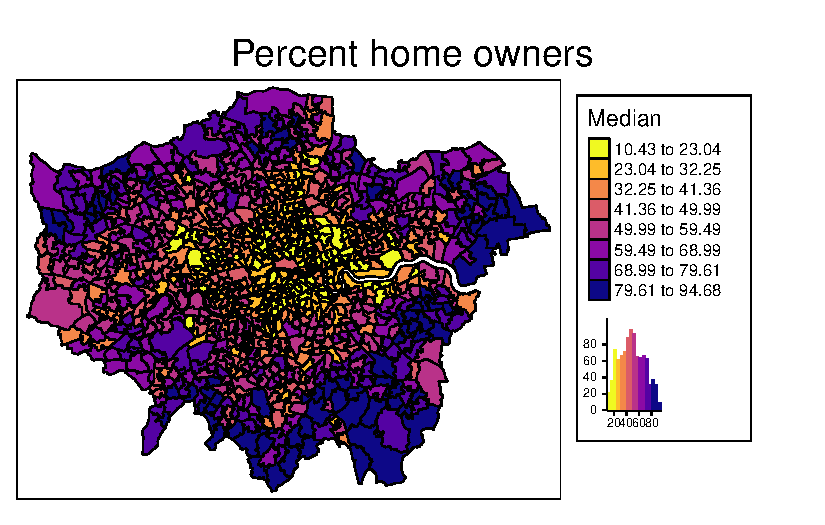
\includegraphics{04_dependence_files/figure-pdf/unnamed-chunk-4-1.pdf}

}

\end{figure}

We definitely see some clusters with spatial units having a low share of
home owner (e.g.~in the city center), and other clusters where home
ownership is high (e.g.~suburbs in the south and east, such as Bromley
or Havering).

However, this is (to some degree) dependent on how we define cutoffs and
coloring of the map: the Modifiable Areal Unit Problem (Wong 2009).

\begin{tcolorbox}[enhanced jigsaw, opacitybacktitle=0.6, left=2mm, leftrule=.75mm, toptitle=1mm, breakable, colback=white, bottomrule=.15mm, colframe=quarto-callout-tip-color-frame, colbacktitle=quarto-callout-tip-color!10!white, coltitle=black, bottomtitle=1mm, titlerule=0mm, title=\textcolor{quarto-callout-tip-color}{\faLightbulb}\hspace{0.5em}{Question}, opacityback=0, arc=.35mm, rightrule=.15mm, toprule=.15mm]

Which of the following three checkerboards has no (or the lowest)
autocorrelation?

\end{tcolorbox}

\includegraphics{fig/segregation.png}

Would your answer be the same if we would aggregate the data to four
larger areas / districts using the average within each of the four
districts?

\hypertarget{morans-i}{%
\subsection{Moran's I}\label{morans-i}}

The most common and well known statistic for spatial dependence or
autocorrelation is Moran's I, which goes back to Moran (1950) and Cliff
and Ord (1972). For more extensive materials on Moran's I see for
instance Kelejian and Piras (2017), Chapter 11.

To calculate Moran's I, we first define a neighbours weights matrix W.

Global Moran's I test statistic: \[      
        \begin{equation} 
        \boldsymbol{\mathbf{I}}  = \frac{N}{S_0}  
        \frac{\sum_i\sum_j w_{ij}(y_i-\bar{y})(y_j-\bar{y})}
            {\sum_i (y_i-\bar{y})^2}, \text{where } S_0 = \sum_{i=1}^N\sum_{j=1}^N w_{ij}
        \end{equation}
\] It is often written with deviations \(z\)

\[      
        \begin{equation} 
        \boldsymbol{\mathbf{I}}  = \frac{N}{S_0}  
        \frac{\sum_i\sum_j w_{ij}(z_i)(z_j)}
            {\sum_i (z_i)^2}, \text{where } S_0 = \sum_{i=1}^N\sum_{j=1}^N w_{ij}
        \end{equation}
\]

Note that in the case of row-standardized weights, \(S_0 = N\). The
\(I\) can be interpreted as: \emph{Relation of the deviation from the
mean value between unit \(i\) and neighbours of unit \(i\)}. Basically,
this measures correlation between neighbouring values.

\begin{itemize}
\item
  Negative values: negative autocorrelation
\item
  Around zero: no autocorrelation
\item
  Positive values: positive autocorrelation
\end{itemize}

To calculate Moran's I, we first need to define the relationship between
units. As in the previous example, we define contiguity weights and
distance-based weights.

\begin{Shaded}
\begin{Highlighting}[]
\CommentTok{\# Contiguity (Queens) neighbours weights}
\NormalTok{queens.nb }\OtherTok{\textless{}{-}} \FunctionTok{poly2nb}\NormalTok{(msoa.spdf, }
                     \AttributeTok{queen =} \ConstantTok{TRUE}\NormalTok{, }
                     \AttributeTok{snap =} \DecValTok{1}\NormalTok{) }\CommentTok{\# we consider points in 1m distance as \textquotesingle{}touching\textquotesingle{}}
\NormalTok{queens.lw }\OtherTok{\textless{}{-}} \FunctionTok{nb2listw}\NormalTok{(queens.nb,}
                      \AttributeTok{style =} \StringTok{"W"}\NormalTok{)}

\CommentTok{\# Neighbours within 3km distance}
\NormalTok{coords }\OtherTok{\textless{}{-}} \FunctionTok{st\_geometry}\NormalTok{(}\FunctionTok{st\_centroid}\NormalTok{(msoa.spdf))}
\end{Highlighting}
\end{Shaded}

\begin{verbatim}
Warning: st_centroid assumes attributes are constant over geometries
\end{verbatim}

\begin{Shaded}
\begin{Highlighting}[]
\NormalTok{dist\_3.nb }\OtherTok{\textless{}{-}} \FunctionTok{dnearneigh}\NormalTok{(coords, }
                        \AttributeTok{d1 =} \DecValTok{0}\NormalTok{, }\AttributeTok{d2 =} \DecValTok{3000}\NormalTok{)}
\NormalTok{idw.lw }\OtherTok{\textless{}{-}} \FunctionTok{nb2listwdist}\NormalTok{(dist\_3.nb,}
                       \AttributeTok{x =}\NormalTok{ coords, }\CommentTok{\# needed for idw}
                       \AttributeTok{type =} \StringTok{"idw"}\NormalTok{, }\CommentTok{\# inverse distance weighting}
                       \AttributeTok{alpha =} \DecValTok{1}\NormalTok{, }\CommentTok{\# the decay parameter for distance weighting}
                       \AttributeTok{style =} \StringTok{"minmax"}\NormalTok{) }\CommentTok{\# for eigenvalue normalization}
\end{Highlighting}
\end{Shaded}

Subsequently, we can calculate the average correlation between
neighbouring units.

For contiguity weights, we get:

\begin{Shaded}
\begin{Highlighting}[]
\CommentTok{\# Global Morans I test of housing values based on contiguity weights}
\FunctionTok{moran.test}\NormalTok{(msoa.spdf}\SpecialCharTok{$}\NormalTok{per\_owner, }\AttributeTok{listw =}\NormalTok{ queens.lw, }\AttributeTok{alternative =} \StringTok{"two.sided"}\NormalTok{)}
\end{Highlighting}
\end{Shaded}

\begin{verbatim}

    Moran I test under randomisation

data:  msoa.spdf$per_owner  
weights: queens.lw    

Moran I statistic standard deviate = 38.161, p-value < 2.2e-16
alternative hypothesis: two.sided
sample estimates:
Moran I statistic       Expectation          Variance 
      0.728706855      -0.001018330       0.000365663 
\end{verbatim}

And for inverse distance weighting, we get:

\begin{Shaded}
\begin{Highlighting}[]
\CommentTok{\# Global Morans I test of housing values based on idw}
\FunctionTok{moran.test}\NormalTok{(msoa.spdf}\SpecialCharTok{$}\NormalTok{per\_owner, }\AttributeTok{listw =}\NormalTok{ idw.lw, }\AttributeTok{alternative =} \StringTok{"two.sided"}\NormalTok{)}
\end{Highlighting}
\end{Shaded}

\begin{verbatim}

    Moran I test under randomisation

data:  msoa.spdf$per_owner  
weights: idw.lw    

Moran I statistic standard deviate = 65.853, p-value < 2.2e-16
alternative hypothesis: two.sided
sample estimates:
Moran I statistic       Expectation          Variance 
     0.6838957350     -0.0010183299      0.0001081719 
\end{verbatim}

Interpretation: In both cases, we have very strong autocorrelation
between neighbouring/closer units (\textasciitilde.7). It barely matters
which of the weights matrices we use. This autocorrelation is highly
significant. we can thus reject the Null that units are independent of
each other (at least at this spatial level and for the share of home
owners).

\hypertarget{residual-based-morans-i}{%
\subsection{Residual-based Moran's I}\label{residual-based-morans-i}}

We can also use the same Moran's I test to inspect spatial
autocorrelation in residuals from an estimated linear model.

Let's start with an intercept only model.

\begin{Shaded}
\begin{Highlighting}[]
\NormalTok{lm0 }\OtherTok{\textless{}{-}} \FunctionTok{lm}\NormalTok{(per\_owner }\SpecialCharTok{\textasciitilde{}} \DecValTok{1}\NormalTok{, msoa.spdf)}
\FunctionTok{lm.morantest}\NormalTok{(lm0, }\AttributeTok{listw =}\NormalTok{ queens.lw, }\AttributeTok{alternative =} \StringTok{"two.sided"}\NormalTok{)}
\end{Highlighting}
\end{Shaded}

\begin{verbatim}

    Global Moran I for regression residuals

data:  
model: lm(formula = per_owner ~ 1, data = msoa.spdf)
weights: queens.lw

Moran I statistic standard deviate = 38.177, p-value < 2.2e-16
alternative hypothesis: two.sided
sample estimates:
Observed Moran I      Expectation         Variance 
    0.7287068548    -0.0010183299     0.0003653613 
\end{verbatim}

This is exactly what we have received in the general case of Moran's I.

Now, lets add some predictors. For instance, the distance to the city
centre, and the population density may be strongly related to the home
ownership rates and explain parts of the spatial dependence.

\begin{Shaded}
\begin{Highlighting}[]
\DocumentationTok{\#\#\# Distance to city center}
\CommentTok{\# Define centre}
\NormalTok{centre }\OtherTok{\textless{}{-}} \FunctionTok{st\_as\_sf}\NormalTok{(}\FunctionTok{data.frame}\NormalTok{(}\AttributeTok{lon =} \SpecialCharTok{{-}}\FloatTok{0.128120855701165}\NormalTok{, }
                              \AttributeTok{lat =} \FloatTok{51.50725909644806}\NormalTok{),}
                   \AttributeTok{coords =} \FunctionTok{c}\NormalTok{(}\StringTok{"lon"}\NormalTok{, }\StringTok{"lat"}\NormalTok{), }
                   \AttributeTok{crs =} \DecValTok{4326}\NormalTok{)}
\CommentTok{\# Reproject}
\NormalTok{centre }\OtherTok{\textless{}{-}} \FunctionTok{st\_transform}\NormalTok{(centre, }\AttributeTok{crs =} \FunctionTok{st\_crs}\NormalTok{(msoa.spdf))}
\CommentTok{\# Calculate distance}
\NormalTok{msoa.spdf}\SpecialCharTok{$}\NormalTok{dist\_centre }\OtherTok{\textless{}{-}} \FunctionTok{as.numeric}\NormalTok{(}\FunctionTok{st\_distance}\NormalTok{(msoa.spdf, centre)) }\SpecialCharTok{/} \DecValTok{1000}
\CommentTok{\# hist(msoa.spdf$dist\_centre)}

\DocumentationTok{\#\#\# Run model with predictors}
\NormalTok{lm1 }\OtherTok{\textless{}{-}} \FunctionTok{lm}\NormalTok{(per\_owner }\SpecialCharTok{\textasciitilde{}}\NormalTok{ dist\_centre }\SpecialCharTok{+}\NormalTok{ POPDEN, msoa.spdf)}
\FunctionTok{lm.morantest}\NormalTok{(lm1, }\AttributeTok{listw =}\NormalTok{ queens.lw, }\AttributeTok{alternative =} \StringTok{"two.sided"}\NormalTok{)}
\end{Highlighting}
\end{Shaded}

\begin{verbatim}

    Global Moran I for regression residuals

data:  
model: lm(formula = per_owner ~ dist_centre + POPDEN, data = msoa.spdf)
weights: queens.lw

Moran I statistic standard deviate = 22.674, p-value < 2.2e-16
alternative hypothesis: two.sided
sample estimates:
Observed Moran I      Expectation         Variance 
    0.4298146060    -0.0024065617     0.0003633607 
\end{verbatim}

There is still considerable auto-correlation in the residuals. However,
we have reduced it by a substantial amount with two very simple control
variables.

\hypertarget{semivariogram}{%
\subsection{Semivariogram}\label{semivariogram}}

The sample variogram \(\gamma(h)\) for distance intervals \(h_i\)
describes the average square difference between the points in this
distance interval:

\begin{equation}\protect\hypertarget{eq-samplevariogram}{}{
\hat{\gamma}(h_i) = \frac{1}{2N(h_i)}\sum_{j=1}^{N(h_i)}(z(s_i)-z(s_i+h'))^2, \ \ h_{i,0} \le h' < h_{i,1}
}\label{eq-samplevariogram}\end{equation}

with the number of available pairs \(N(h_i)\) in each distance interval
\(h_i\). Basically, \emph{it is the variance within each distance
interval}.

For more information, see for instance the
\href{https://zia207.github.io/geospatial-r-github.io/semivariogram-modeling.html}{Geospatial
Data Science in R} by Zia Ahmed or Pebesma and Bivand (2023).

To calculate the empirical semi-vriogram, we can use the package
\texttt{gstat} with the function \texttt{variogram()}.

\begin{Shaded}
\begin{Highlighting}[]
\CommentTok{\# Variogram No2}
\NormalTok{v.no2 }\OtherTok{\textless{}{-}} \FunctionTok{variogram}\NormalTok{(no2 }\SpecialCharTok{\textasciitilde{}} \DecValTok{1}\NormalTok{, msoa.spdf)}
\FunctionTok{plot}\NormalTok{(v.no2, }\AttributeTok{xlim =} \FunctionTok{c}\NormalTok{(}\DecValTok{0}\NormalTok{, }\FloatTok{1.075} \SpecialCharTok{*} \FunctionTok{max}\NormalTok{(v.no2}\SpecialCharTok{$}\NormalTok{dist)),}
     \AttributeTok{ylim =} \FunctionTok{c}\NormalTok{(}\SpecialCharTok{{-}}\DecValTok{10}\NormalTok{, }\FloatTok{1.05} \SpecialCharTok{*} \FunctionTok{max}\NormalTok{(v.no2}\SpecialCharTok{$}\NormalTok{gamma)))}
\end{Highlighting}
\end{Shaded}

\begin{figure}[H]

{\centering 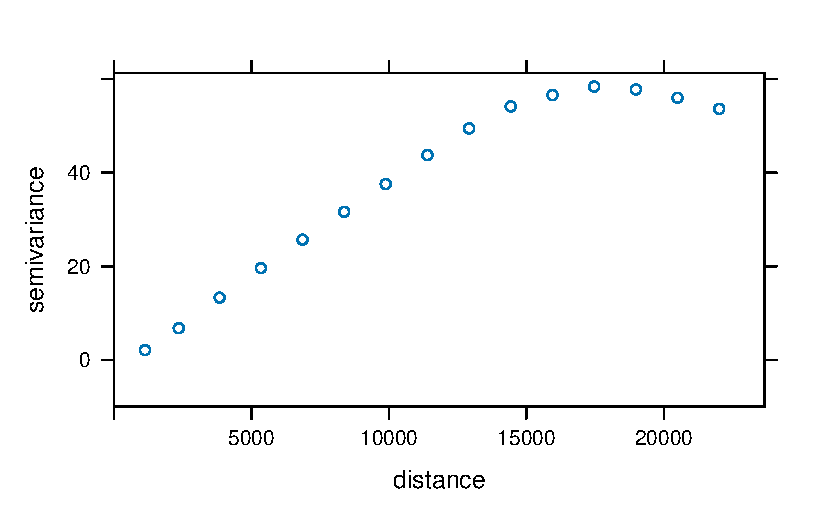
\includegraphics{04_dependence_files/figure-pdf/unnamed-chunk-10-1.pdf}

}

\end{figure}

Above graphs shows that the variance within each distance interval
gradually increases, up to a distance of \textasciitilde{} 18km, and
then level off at a relative constant level. Lower variances within
lower values of distances means that observations are more similar to
each other the closer they are.

We can also try to fit a model that resembles the spatial structure.
This becomes important when we want to perform spatial interpolation
(e.g.~to impute missings).

\begin{figure}

{\centering \includegraphics{fig/Semi_variogram.png}

}

\caption{Theoretical exponential semi-variogram model. Source:
https://www.aspexit.com/variogram-and-spatial-autocorrelation}

\end{figure}

\begin{Shaded}
\begin{Highlighting}[]
\CommentTok{\# Intial parameter set by eye esitmation}
\NormalTok{m.no2 }\OtherTok{\textless{}{-}} \FunctionTok{vgm}\NormalTok{(}\DecValTok{60}\NormalTok{, }\StringTok{"Cir"}\NormalTok{, }\DecValTok{20000}\NormalTok{, }\DecValTok{0}\NormalTok{)  }\CommentTok{\# Sill, model, range, nugget}
\CommentTok{\# least square fit}
\NormalTok{m.f.v.no2 }\OtherTok{\textless{}{-}} \FunctionTok{fit.variogram}\NormalTok{(v.no2, m.no2)}
\end{Highlighting}
\end{Shaded}

\begin{Shaded}
\begin{Highlighting}[]
\DocumentationTok{\#\#\#\# Plot varigram and fitted model:}
\FunctionTok{plot}\NormalTok{(v.no2, }\AttributeTok{pl =} \ConstantTok{FALSE}\NormalTok{, }
     \AttributeTok{model =}\NormalTok{ m.f.v.no2,}
     \AttributeTok{col=}\StringTok{"blue"}\NormalTok{, }
     \AttributeTok{cex =} \FloatTok{0.9}\NormalTok{, }
     \AttributeTok{lwd =} \FloatTok{0.5}\NormalTok{,}
     \AttributeTok{lty =} \DecValTok{1}\NormalTok{,}
     \AttributeTok{pch =} \DecValTok{19}\NormalTok{,}
     \AttributeTok{main =} \StringTok{"Variogram and Fitted Model"}\NormalTok{,}
     \AttributeTok{xlab =} \StringTok{"Distance (m)"}\NormalTok{,}
     \AttributeTok{ylab =} \StringTok{"Semivariance"}\NormalTok{)}
\end{Highlighting}
\end{Shaded}

\begin{figure}[H]

{\centering 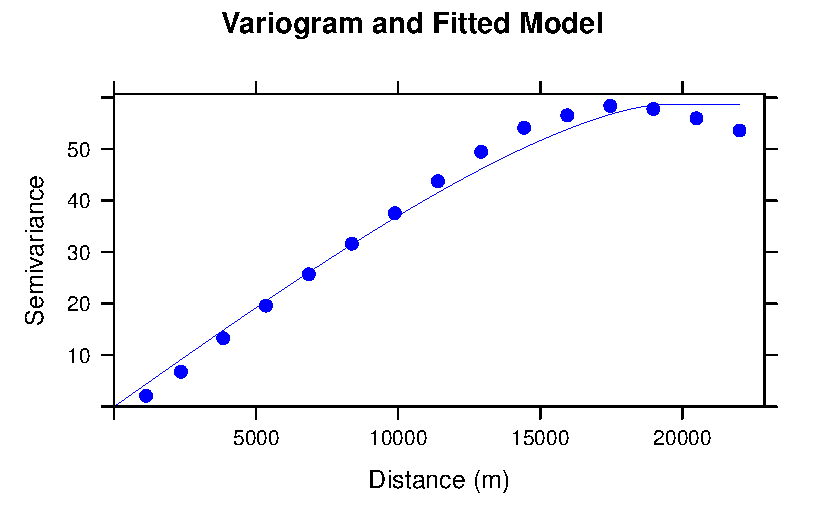
\includegraphics{04_dependence_files/figure-pdf/unnamed-chunk-12-1.pdf}

}

\end{figure}

\hypertarget{example}{%
\subsection{Example}\label{example}}

\begin{figure}

{\centering 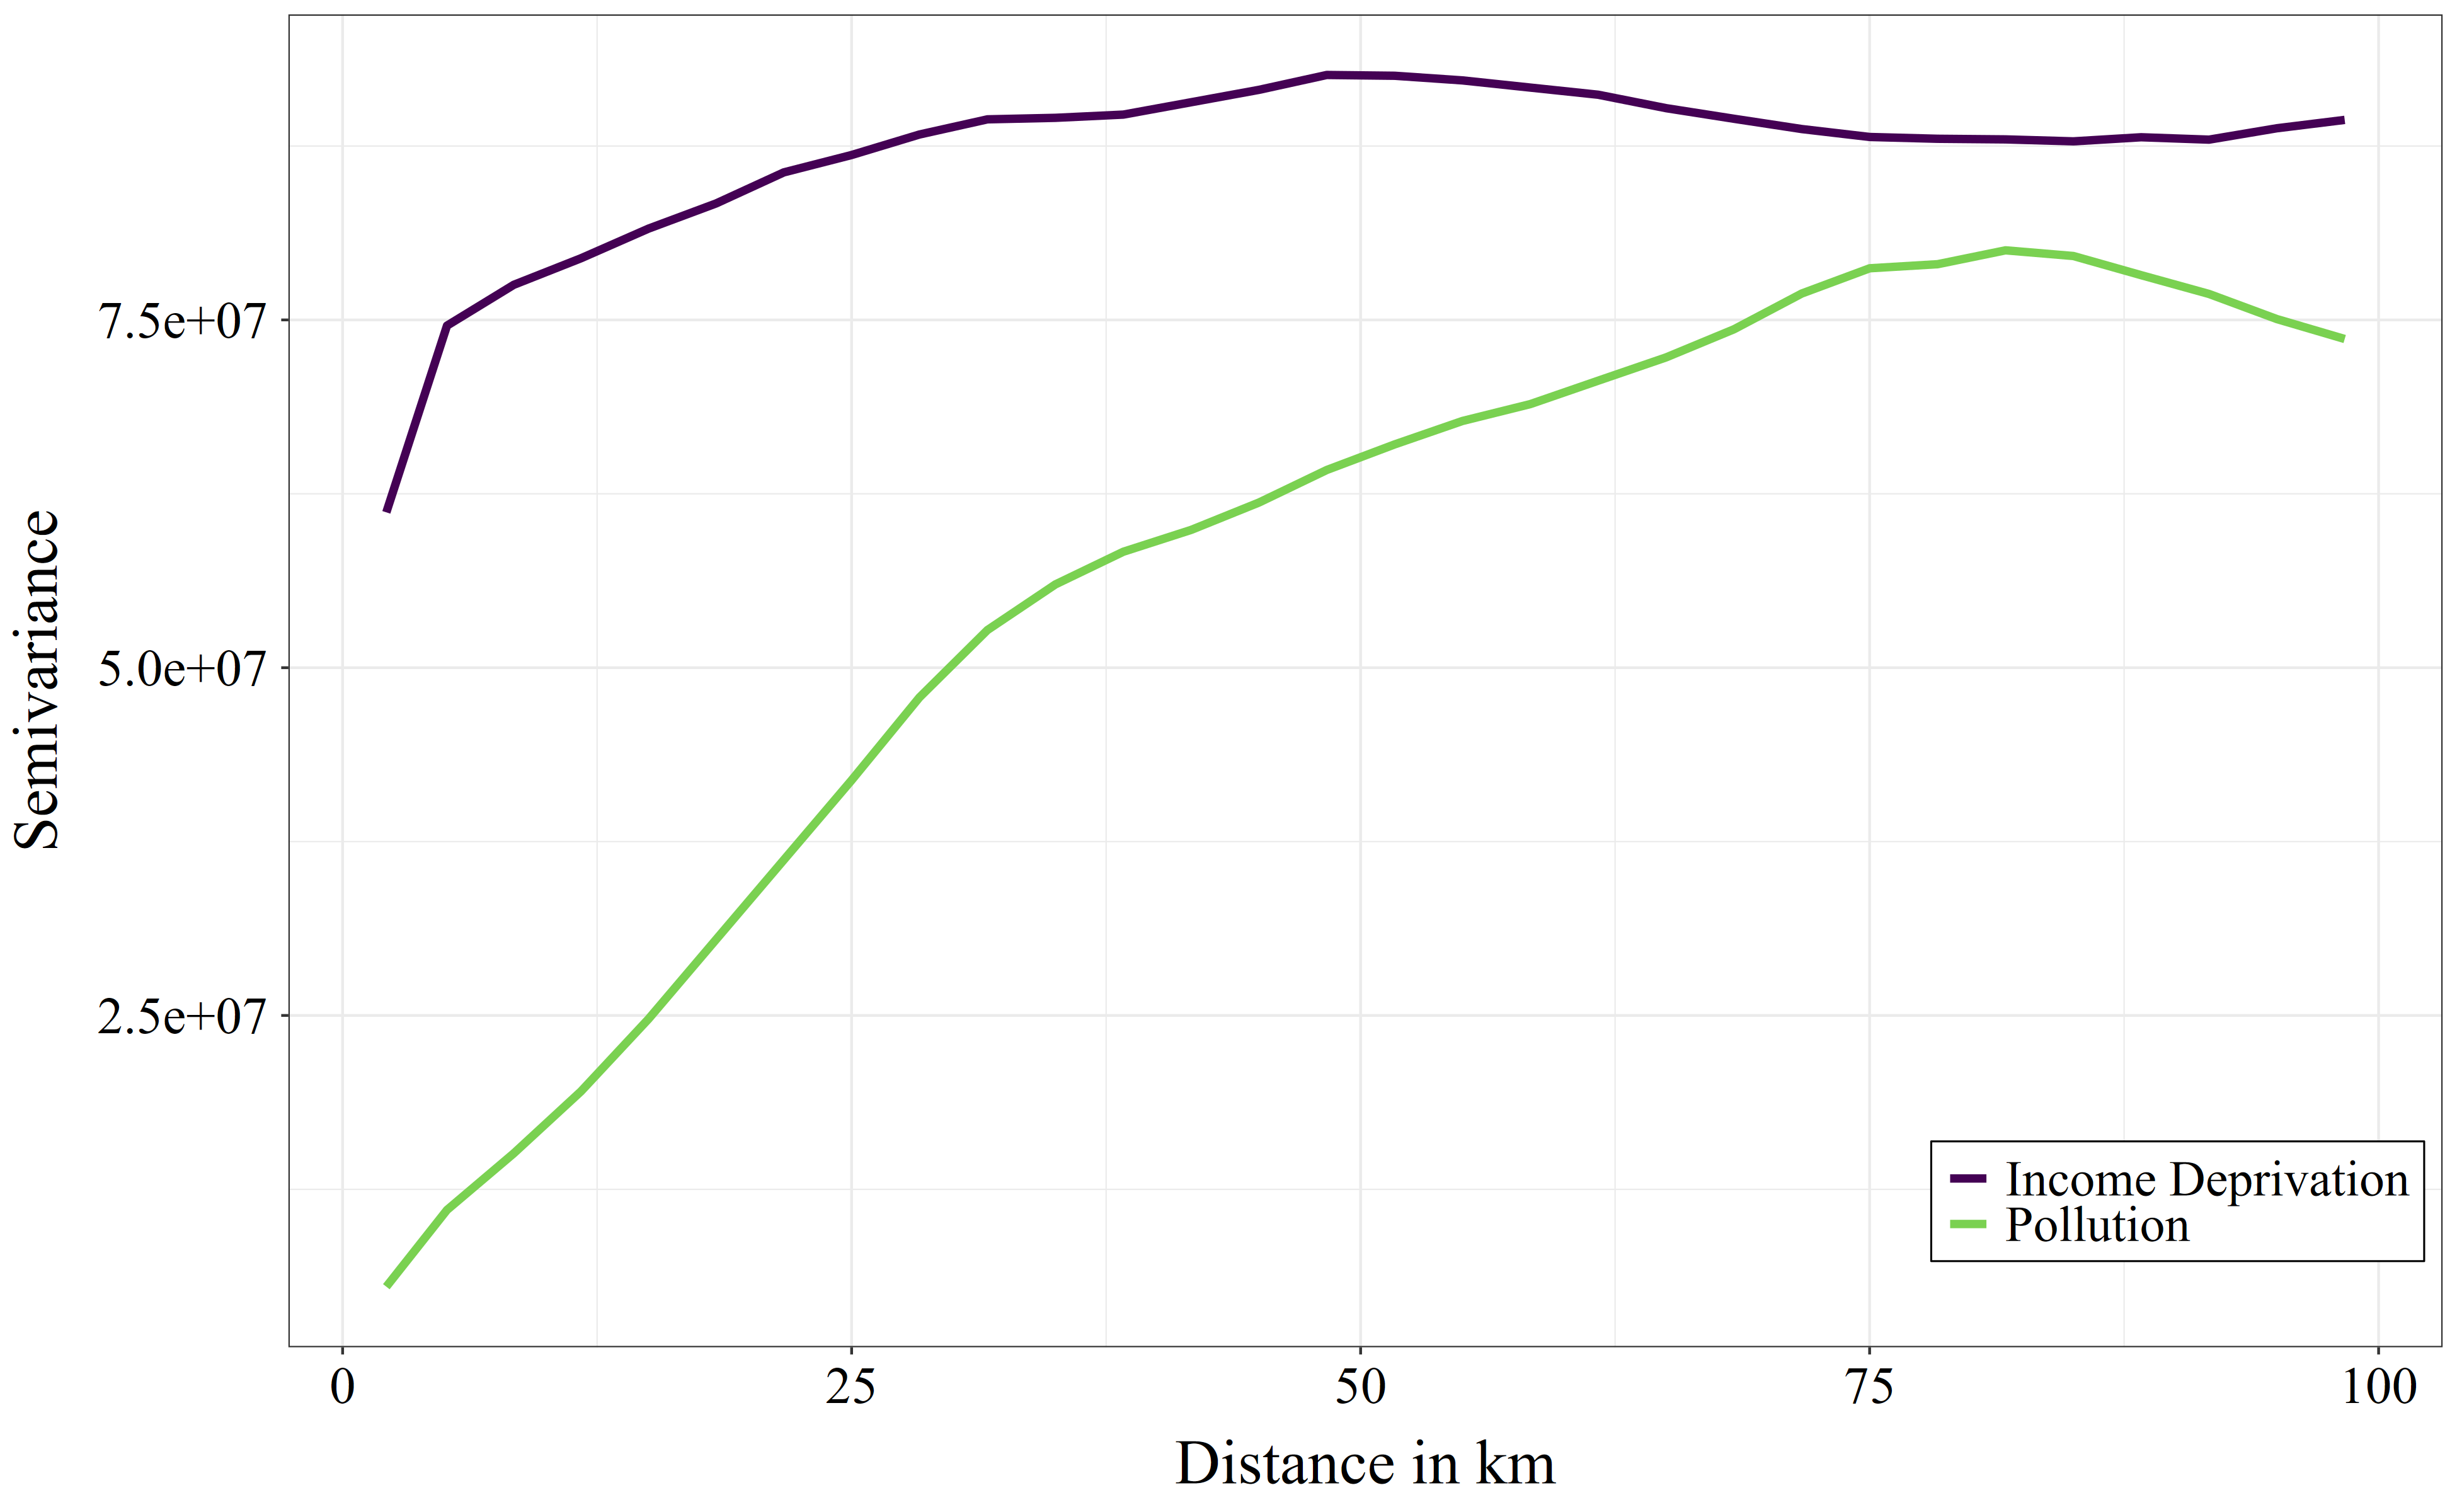
\includegraphics{fig/Semivariogram_2019.png}

}

\caption{Semivariogram of Air pollution and income deprivation in
England on the LSOA level for 2019.}

\end{figure}

When looking at approx. 10 km distance: the variance in income
deprivation is nearly as high when looking at areas within 10km as it
would be when looking at areas within 100km distance. This indicates
that income deprivation is very local and varies already within smaller
areas such as within cities or district. Air pollution, in contrast, has
a much lower variance within 10km distances than we would find when
looking at the data within 100km distance. This indicates that air
pollution has stronger large-scale spatial patterns. When moving locally
(e.g.~within 10km) to a random location, it would be more difficult to
improve in air pollution than it would be to improve in income
deprivation.

\hypertarget{local-autocorrelation}{%
\section{Local Autocorrelation}\label{local-autocorrelation}}

The Global Moran's I statistic above summarizes the spatial pattern by a
single value. Although this is helpful to get a feeling of the strength
of the general spatial association, it is often more helpful to inspect
the spatial pattern in more detail.

The most prominent measure is the Local Indicators of Spatial
Association (LISA) (Anselin 1995). LISA measures assess the importance
and significance of a satistic at different spatial locations. For more
information see for instance the
\href{https://geodacenter.github.io/workbook/6a_local_auto/lab6a.html}{GeoData
Materials} by Luc Anselin.

For instance, we can use the Moran Plot to identify how single (pairs
of) units contribute to the overall dependence.

\begin{Shaded}
\begin{Highlighting}[]
\NormalTok{mp }\OtherTok{\textless{}{-}} \FunctionTok{moran.plot}\NormalTok{(msoa.spdf}\SpecialCharTok{$}\NormalTok{per\_owner, queens.lw)}
\end{Highlighting}
\end{Shaded}

\begin{figure}[H]

{\centering 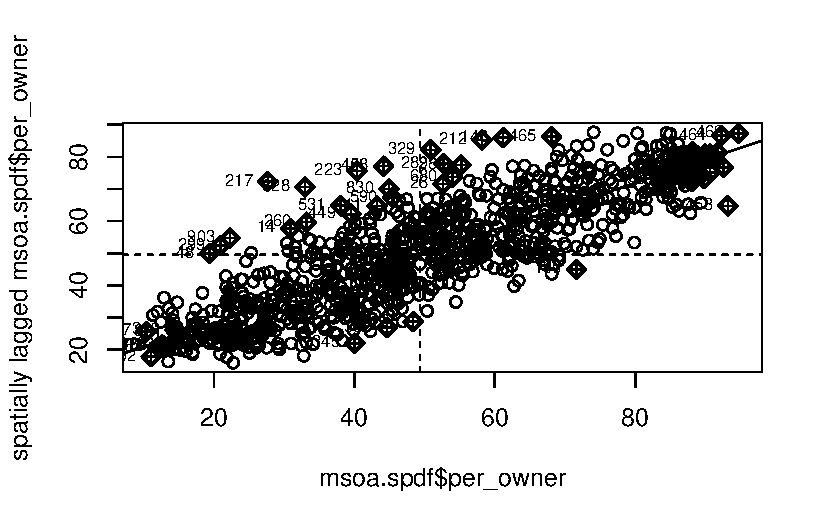
\includegraphics{04_dependence_files/figure-pdf/unnamed-chunk-13-1.pdf}

}

\end{figure}

In the lower left corner, we see units with a low-low share of home
ownership: focal and neighbouring units have a low share of home owners.
In the top right corner, by contrast, we see high-high units.

And we can plot influence values on the Overall Moran statistic.

\begin{Shaded}
\begin{Highlighting}[]
\NormalTok{msoa.spdf}\SpecialCharTok{$}\NormalTok{hat\_value }\OtherTok{\textless{}{-}}\NormalTok{ mp}\SpecialCharTok{$}\NormalTok{hat }
\NormalTok{mp1 }\OtherTok{\textless{}{-}}  \FunctionTok{tm\_shape}\NormalTok{(msoa.spdf) }\SpecialCharTok{+} 
  \FunctionTok{tm\_fill}\NormalTok{(}\AttributeTok{col =} \StringTok{"hat\_value"}\NormalTok{, }
          \AttributeTok{palette =} \FunctionTok{viridis}\NormalTok{(}\AttributeTok{n =} \DecValTok{10}\NormalTok{, }\AttributeTok{direction =} \SpecialCharTok{{-}}\DecValTok{1}\NormalTok{, }\AttributeTok{option =} \StringTok{"C"}\NormalTok{),}
\NormalTok{          ) }\SpecialCharTok{+}
  \FunctionTok{tm\_borders}\NormalTok{(}\AttributeTok{col =} \StringTok{"white"}\NormalTok{, }\AttributeTok{lwd =} \FloatTok{0.5}\NormalTok{, }\AttributeTok{alpha =} \FloatTok{0.5}\NormalTok{) }\SpecialCharTok{+}
  \FunctionTok{tm\_layout}\NormalTok{(}\AttributeTok{frame =} \ConstantTok{FALSE}\NormalTok{,}
            \AttributeTok{legend.frame =} \ConstantTok{TRUE}\NormalTok{, }\AttributeTok{legend.bg.color =} \ConstantTok{TRUE}\NormalTok{,}
            \AttributeTok{legend.position =} \FunctionTok{c}\NormalTok{(}\StringTok{"right"}\NormalTok{, }\StringTok{"bottom"}\NormalTok{),}
            \AttributeTok{legend.outside =} \ConstantTok{FALSE}\NormalTok{,}
            \AttributeTok{main.title =} \StringTok{"Influence"}\NormalTok{, }
            \AttributeTok{main.title.position =} \StringTok{"center"}\NormalTok{,}
            \AttributeTok{main.title.size =} \FloatTok{1.6}\NormalTok{,}
            \AttributeTok{legend.title.size =} \FloatTok{0.8}\NormalTok{,}
            \AttributeTok{legend.text.size =} \FloatTok{0.8}\NormalTok{)}

\NormalTok{mp1}
\end{Highlighting}
\end{Shaded}

\begin{figure}[H]

{\centering 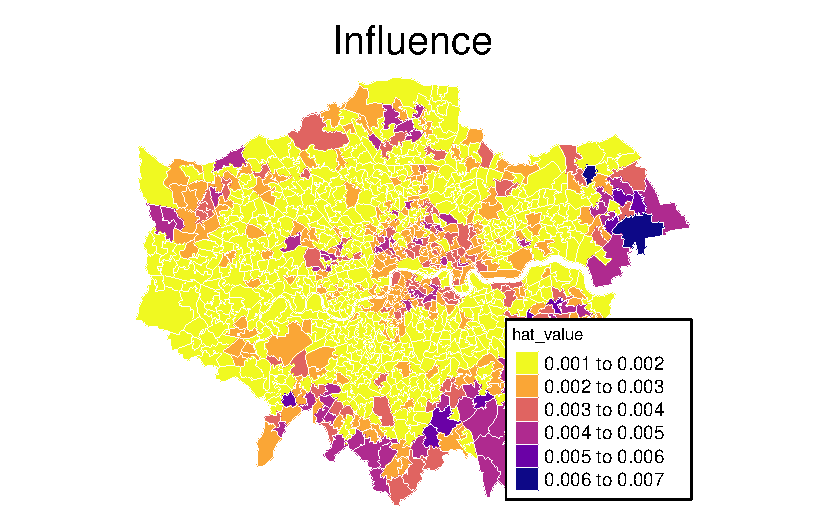
\includegraphics{04_dependence_files/figure-pdf/unnamed-chunk-14-1.pdf}

}

\end{figure}

\hypertarget{local-morans-i}{%
\section{Local Moran's I}\label{local-morans-i}}

Local Moran's I is a local version of the overall Moran's I to identify
local clusters and local spatial outliers (Anselin 1995). The Local
Moran's I is just a local version which is calculated for each location:

\[      
        \begin{equation} 
        \boldsymbol{\mathbf{I}}_i  =  
        \frac{z_i \sum_j w_{ij}z_j}
            {\sum_i (z_i)^2 / (n-1)}, \text{where }
        \end{equation}
\] We use the unfction \texttt{localmoran()} to calculate the local test
statistic .

\begin{Shaded}
\begin{Highlighting}[]
\NormalTok{loci }\OtherTok{\textless{}{-}} \FunctionTok{localmoran}\NormalTok{(msoa.spdf}\SpecialCharTok{$}\NormalTok{per\_owner, }\AttributeTok{listw =}\NormalTok{ queens.lw)}
\FunctionTok{head}\NormalTok{(loci)}
\end{Highlighting}
\end{Shaded}

\begin{verbatim}
           Ii          E.Ii      Var.Ii       Z.Ii Pr(z != E(Ii))
1  0.42322928 -1.285364e-04 0.011367934  3.9706976   7.166249e-05
2 -0.12775982 -2.229957e-05 0.003634711 -2.1187688   3.411001e-02
3  0.38111534 -6.569549e-04 0.091630752  1.2611995   2.072370e-01
4  1.02874685 -1.428679e-03 0.279333375  1.9491704   5.127507e-02
5  0.08553291 -2.108521e-04 0.041275789  0.4220412   6.729949e-01
6 -0.24014505 -2.228818e-04 0.036321252 -1.2588964   2.080678e-01
\end{verbatim}

It also has an attribute with the Moran plot quadrant of each
observation.

\begin{Shaded}
\begin{Highlighting}[]
\FunctionTok{head}\NormalTok{(}\FunctionTok{attr}\NormalTok{(loci, }\StringTok{"quadr"}\NormalTok{))}
\end{Highlighting}
\end{Shaded}

\begin{verbatim}
       mean    median     pysal
1   Low-Low   Low-Low   Low-Low
2  Low-High  Low-High  Low-High
3 High-High High-High High-High
4 High-High High-High High-High
5 High-High High-High High-High
6  Low-High  Low-High  Low-High
\end{verbatim}

This returns a data.frame with local moran statisic, the expectation of
local moran statistic, its variance, and a p value for the satistical
significance of each unit. Note that we obviously have a problem of
multiple comparisons here and thus may want to correct the significance
level, e.g.~by Bonferroni adjustment (R. Bivand and Wong 2018).

\begin{Shaded}
\begin{Highlighting}[]
\NormalTok{loci.df }\OtherTok{\textless{}{-}} \FunctionTok{data.frame}\NormalTok{(loci)}
\FunctionTok{names}\NormalTok{(loci.df) }\OtherTok{\textless{}{-}} \FunctionTok{gsub}\NormalTok{(}\StringTok{"}\SpecialCharTok{\textbackslash{}\textbackslash{}}\StringTok{."}\NormalTok{, }\StringTok{""}\NormalTok{, }\FunctionTok{names}\NormalTok{(loci.df))}
\NormalTok{msoa.spdf}\SpecialCharTok{$}\NormalTok{loci }\OtherTok{\textless{}{-}}\NormalTok{ loci.df}\SpecialCharTok{$}\NormalTok{Ii}
\NormalTok{msoa.spdf}\SpecialCharTok{$}\NormalTok{p\_value }\OtherTok{\textless{}{-}}\NormalTok{ loci.df}\SpecialCharTok{$}\NormalTok{PrzEIi}
\NormalTok{msoa.spdf}\SpecialCharTok{$}\NormalTok{p\_value\_adj1 }\OtherTok{\textless{}{-}} \FunctionTok{p.adjust}\NormalTok{(loci.df}\SpecialCharTok{$}\NormalTok{PrzEIi, }\StringTok{"BY"}\NormalTok{)}
\NormalTok{msoa.spdf}\SpecialCharTok{$}\NormalTok{p\_value\_adj2 }\OtherTok{\textless{}{-}} \FunctionTok{p.adjust}\NormalTok{(loci.df}\SpecialCharTok{$}\NormalTok{PrzEIi, }\StringTok{"bonferroni"}\NormalTok{)}
\end{Highlighting}
\end{Shaded}

\begin{Shaded}
\begin{Highlighting}[]
\NormalTok{mp1 }\OtherTok{\textless{}{-}}  \FunctionTok{tm\_shape}\NormalTok{(msoa.spdf) }\SpecialCharTok{+} 
  \FunctionTok{tm\_fill}\NormalTok{(}\AttributeTok{col =} \FunctionTok{c}\NormalTok{(}\StringTok{"loci"}\NormalTok{, }\StringTok{"p\_value"}\NormalTok{, }\StringTok{"p\_value\_adj1"}\NormalTok{, }\StringTok{"p\_value\_adj2"}\NormalTok{),}
          \AttributeTok{palette =} \FunctionTok{viridis}\NormalTok{(}\AttributeTok{n =} \DecValTok{10}\NormalTok{, }\AttributeTok{direction =} \SpecialCharTok{{-}}\DecValTok{1}\NormalTok{, }\AttributeTok{option =} \StringTok{"C"}\NormalTok{),}
\NormalTok{          ) }\SpecialCharTok{+}
  \FunctionTok{tm\_borders}\NormalTok{(}\AttributeTok{col =} \StringTok{"white"}\NormalTok{, }\AttributeTok{lwd =} \FloatTok{0.5}\NormalTok{, }\AttributeTok{alpha =} \FloatTok{0.5}\NormalTok{) }\SpecialCharTok{+}
  \FunctionTok{tm\_layout}\NormalTok{(}\AttributeTok{frame =} \ConstantTok{FALSE}\NormalTok{,}
            \AttributeTok{legend.frame =} \ConstantTok{TRUE}\NormalTok{, }\AttributeTok{legend.bg.color =} \ConstantTok{TRUE}\NormalTok{,}
            \AttributeTok{legend.position =} \FunctionTok{c}\NormalTok{(}\StringTok{"left"}\NormalTok{, }\StringTok{"bottom"}\NormalTok{),}
            \AttributeTok{legend.outside =} \ConstantTok{FALSE}\NormalTok{,}
            \AttributeTok{main.title =} \StringTok{"Local Morans I"}\NormalTok{, }
            \AttributeTok{main.title.position =} \StringTok{"center"}\NormalTok{,}
            \AttributeTok{main.title.size =} \FloatTok{1.6}\NormalTok{,}
            \AttributeTok{legend.title.size =} \FloatTok{0.8}\NormalTok{,}
            \AttributeTok{legend.text.size =} \FloatTok{0.8}\NormalTok{,}
            \AttributeTok{panel.labels =} \FunctionTok{c}\NormalTok{(}\StringTok{"Morans I"}\NormalTok{,}
                               \StringTok{"P value"}\NormalTok{,}
                               \StringTok{"p value BY"}\NormalTok{,}
                             \StringTok{"p value Bonferroni"}\NormalTok{))}

\NormalTok{mp1}
\end{Highlighting}
\end{Shaded}

\begin{figure}[H]

{\centering 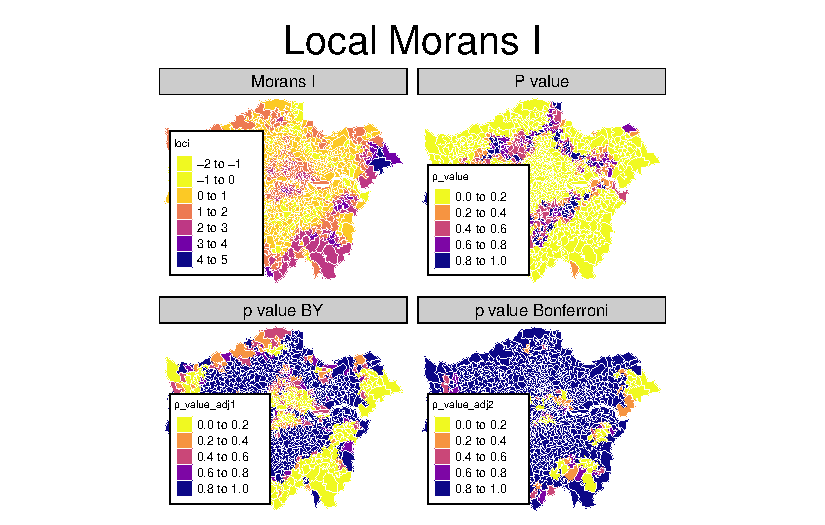
\includegraphics{04_dependence_files/figure-pdf/unnamed-chunk-18-1.pdf}

}

\end{figure}

Something you can often see are so called LISA hotspot maps. They are
based on the same idea as the moran plot, and show cluster of high-high
and low-low values. We can use the hotspot function to identify the
clusters, with a cutoff for singificance and the adjustment for multiple
testing.

\begin{Shaded}
\begin{Highlighting}[]
\CommentTok{\# Calculate clusters}
\NormalTok{msoa.spdf}\SpecialCharTok{$}\NormalTok{lisa\_cluster }\OtherTok{\textless{}{-}} \FunctionTok{hotspot}\NormalTok{(loci, }
                                  \StringTok{"Pr(z != E(Ii))"}\NormalTok{, }
                                  \AttributeTok{cutoff =} \FloatTok{0.05}\NormalTok{, }
                                  \AttributeTok{quadrant.type =} \StringTok{"mean"}\NormalTok{,}
                                  \AttributeTok{p.adjust =} \StringTok{"BY"}\NormalTok{)}

\CommentTok{\# Map}
\NormalTok{mp1 }\OtherTok{\textless{}{-}}  \FunctionTok{tm\_shape}\NormalTok{(msoa.spdf) }\SpecialCharTok{+} 
  \FunctionTok{tm\_fill}\NormalTok{(}\AttributeTok{col =} \FunctionTok{c}\NormalTok{(}\StringTok{"lisa\_cluster"}\NormalTok{),}
          \AttributeTok{palette =} \FunctionTok{viridis}\NormalTok{(}\AttributeTok{n =} \DecValTok{3}\NormalTok{, }\AttributeTok{direction =} \SpecialCharTok{{-}}\DecValTok{1}\NormalTok{, }\AttributeTok{option =} \StringTok{"D"}\NormalTok{),}
          \AttributeTok{colorNA =} \StringTok{"white"}\NormalTok{) }\SpecialCharTok{+}
  \FunctionTok{tm\_borders}\NormalTok{(}\AttributeTok{col =} \StringTok{"grey70"}\NormalTok{, }\AttributeTok{lwd =} \FloatTok{0.5}\NormalTok{, }\AttributeTok{alpha =} \FloatTok{0.5}\NormalTok{) }\SpecialCharTok{+}
  \FunctionTok{tm\_layout}\NormalTok{(}\AttributeTok{frame =} \ConstantTok{FALSE}\NormalTok{,}
            \AttributeTok{legend.frame =} \ConstantTok{TRUE}\NormalTok{, }\AttributeTok{legend.bg.color =} \ConstantTok{TRUE}\NormalTok{,}
            \AttributeTok{legend.position =} \FunctionTok{c}\NormalTok{(}\StringTok{"left"}\NormalTok{, }\StringTok{"bottom"}\NormalTok{),}
            \AttributeTok{legend.outside =} \ConstantTok{FALSE}\NormalTok{,}
            \AttributeTok{main.title =} \StringTok{"Home Ownership }\SpecialCharTok{\textbackslash{}n}\StringTok{ LISA Clusters p(BY) \textless{} 0.05"}\NormalTok{, }
            \AttributeTok{main.title.position =} \StringTok{"center"}\NormalTok{,}
            \AttributeTok{main.title.size =} \FloatTok{1.6}\NormalTok{,}
            \AttributeTok{legend.title.size =} \FloatTok{0.8}\NormalTok{,}
            \AttributeTok{legend.text.size =} \FloatTok{0.8}\NormalTok{,)}

\NormalTok{mp1}
\end{Highlighting}
\end{Shaded}

\begin{figure}[H]

{\centering 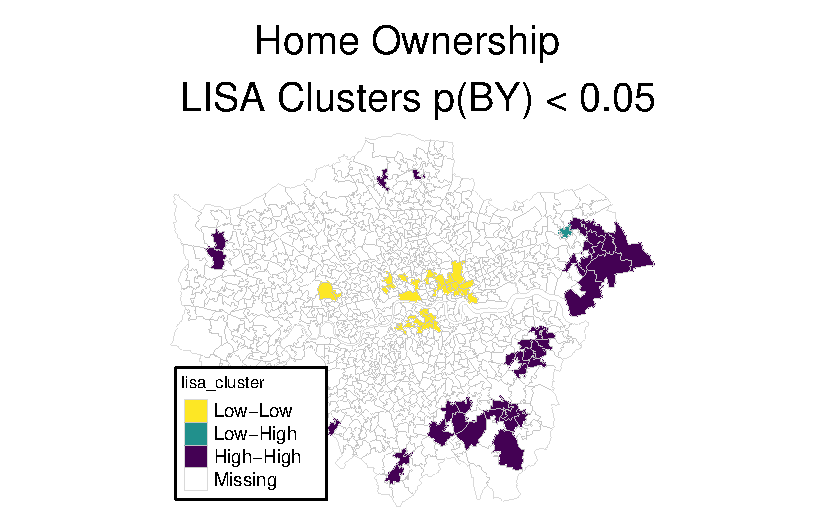
\includegraphics{04_dependence_files/figure-pdf/unnamed-chunk-19-1.pdf}

}

\end{figure}

Note that it is not suggested to interpret those cluster as singificant
in the strict statistical sense. Pebesma and Bivand (2023) suggest to
speak of \emph{interesting clusters}. After all, this is an explorative
approach. Nevertheless, it can help to identify spatial patterns and
clusters.

There are more ways of calculating these hotspot maps and more choices
on the cutoffs and calculation of the statistical significance. For more
materials see \href{https://r-spatial.org/book/15-Measures.html}{Chapter
15} of Pebesma and Bivand (2023).

\hypertarget{example-1}{%
\section{Example}\label{example-1}}

\hypertarget{tate.2021}{%
\subsection*{Tate.2021}\label{tate.2021}}
\addcontentsline{toc}{subsection}{Tate.2021}

\emph{This study explores the geography of flood exposure and social
vulnerability in the conterminous United States based on spatial
analysis of fluvial and pluvial flood extent, land cover, and social
vulnerability.}

\emph{Mobile homes and racial minorities are most overrepresented in
hotspots compared to elsewhere. The results identify priority locations
where interventions can mitigate both physical and social aspects of
flood vulnerability.}

\includegraphics{fig/Tate.png}

\hypertarget{exercises-1}{%
\section{Exercises}\label{exercises-1}}

\begin{enumerate}
\def\labelenumi{\arabic{enumi}.}
\item
  Please calculate a neighbours weights matrix of the nearest 10
  neighbours (see \texttt{spdep::knearneigh()}), and create a listw
  object using row normalization.
\item
  Chose another characteristics from the data (e.g.~ethnic groups or
  house prices) and calculate global Moran's I for it.
\item
  Produce a LISA cluster map for the characteristic you have chosen.
\end{enumerate}

\bookmarksetup{startatroot}

\hypertarget{spatial-regression-models}{%
\chapter{Spatial Regression Models}\label{spatial-regression-models}}

\newcommand{\Exp}{\mathrm{E}}
\newcommand\given[1][]{\:#1\vert\:}
\newcommand{\Cov}{\mathrm{Cov}}
\newcommand{\Var}{\mathrm{Var}}
\newcommand{\rank}{\mathrm{rank}}
\newcommand{\bm}[1]{\boldsymbol{\mathbf{#1}}}
\newcommand{\tr}{\mathrm{tr}}
\newcommand{\plim}{\operatornamewithlimits{plim}}
\newcommand{\diag}{\mathrm{diag}}

\hypertarget{required-packages-5}{%
\subsection*{Required packages}\label{required-packages-5}}
\addcontentsline{toc}{subsection}{Required packages}

\begin{Shaded}
\begin{Highlighting}[]
\NormalTok{pkgs }\OtherTok{\textless{}{-}} \FunctionTok{c}\NormalTok{(}\StringTok{"sf"}\NormalTok{, }\StringTok{"mapview"}\NormalTok{, }\StringTok{"spdep"}\NormalTok{, }\StringTok{"spatialreg"}\NormalTok{, }\StringTok{"tmap"}\NormalTok{, }\StringTok{"viridisLite"}\NormalTok{) }\CommentTok{\# note: load spdep first, then spatialreg}
\FunctionTok{lapply}\NormalTok{(pkgs, require, }\AttributeTok{character.only =} \ConstantTok{TRUE}\NormalTok{)}
\end{Highlighting}
\end{Shaded}

\hypertarget{session-info-5}{%
\subsection*{Session info}\label{session-info-5}}
\addcontentsline{toc}{subsection}{Session info}

\begin{Shaded}
\begin{Highlighting}[]
\FunctionTok{sessionInfo}\NormalTok{()}
\end{Highlighting}
\end{Shaded}

\begin{verbatim}
R version 4.4.1 (2024-06-14 ucrt)
Platform: x86_64-w64-mingw32/x64
Running under: Windows 11 x64 (build 22631)

Matrix products: default


locale:
[1] LC_COLLATE=English_United Kingdom.utf8 
[2] LC_CTYPE=English_United Kingdom.utf8   
[3] LC_MONETARY=English_United Kingdom.utf8
[4] LC_NUMERIC=C                           
[5] LC_TIME=English_United Kingdom.utf8    

time zone: Europe/Berlin
tzcode source: internal

attached base packages:
[1] stats     graphics  grDevices utils     datasets  methods   base     

other attached packages:
[1] viridisLite_0.4.2 tmap_3.3-4        spatialreg_1.3-4  Matrix_1.7-0     
[5] spdep_1.3-5       spData_2.3.1      mapview_2.11.2    sf_1.0-16        

loaded via a namespace (and not attached):
 [1] xfun_0.45          raster_3.6-26      htmlwidgets_1.6.4  lattice_0.22-6    
 [5] tools_4.4.1        crosstalk_1.2.1    LearnBayes_2.15.1  parallel_4.4.1    
 [9] stats4_4.4.1       sandwich_3.1-0     proxy_0.4-27       KernSmooth_2.23-24
[13] satellite_1.0.5    RColorBrewer_1.1-3 leaflet_2.2.2      lifecycle_1.0.4   
[17] compiler_4.4.1     deldir_2.0-4       munsell_0.5.1      terra_1.7-78      
[21] codetools_0.2-20   leafsync_0.1.0     stars_0.6-5        htmltools_0.5.8.1 
[25] class_7.3-22       MASS_7.3-60.2      classInt_0.4-10    lwgeom_0.2-14     
[29] wk_0.9.1           abind_1.4-5        boot_1.3-30        multcomp_1.4-25   
[33] nlme_3.1-164       digest_0.6.35      mvtnorm_1.2-5      splines_4.4.1     
[37] fastmap_1.2.0      grid_4.4.1         colorspace_2.1-0   cli_3.6.2         
[41] magrittr_2.0.3     base64enc_0.1-3    dichromat_2.0-0.1  XML_3.99-0.16.1   
[45] survival_3.6-4     leafem_0.2.3       TH.data_1.1-2      e1071_1.7-14      
[49] scales_1.3.0       sp_2.1-4           rmarkdown_2.27     zoo_1.8-12        
[53] png_0.1-8          coda_0.19-4.1      evaluate_0.24.0    knitr_1.47        
[57] tmaptools_3.1-1    s2_1.1.6           rlang_1.1.4        Rcpp_1.0.12       
[61] glue_1.7.0         DBI_1.2.3          rstudioapi_0.16.0  jsonlite_1.8.8    
[65] R6_2.5.1           units_0.8-5       
\end{verbatim}

\hypertarget{reload-data-from-pervious-session-4}{%
\subsection*{Reload data from pervious
session}\label{reload-data-from-pervious-session-4}}
\addcontentsline{toc}{subsection}{Reload data from pervious session}

\begin{Shaded}
\begin{Highlighting}[]
\FunctionTok{load}\NormalTok{(}\StringTok{"\_data/msoa2\_spatial.RData"}\NormalTok{)}
\end{Highlighting}
\end{Shaded}

There are various techniques to model spatial dependence and spatial
processes (LeSage and Pace 2009). Here, we will just cover a few of the
most common techniques / econometric models. One advantage of the most
basic spatial model (SLX) is that this method can easily be incorporated
in a variety of other methodologies, such as machine learning
approaches.

For more in-depth materials see LeSage and Pace (2009) and Kelejian and
Piras (2017). Franzese and Hays (2007), Halleck Vega and Elhorst (2015),
LeSage (2014a), Rüttenauer (2022), and Wimpy, Whitten, and Williams
(2021) provide article-length introductions. Rüttenauer (2024) is a
handbook chapter based on the materials of this workshop.

\hypertarget{why-do-we-need-spatial-regression-models}{%
\section{Why do we need spatial regression
models}\label{why-do-we-need-spatial-regression-models}}

\hypertarget{non-spatial-ols}{%
\subsection{Non-spatial OLS}\label{non-spatial-ols}}

Let us start with a linear model, where \(\boldsymbol{\mathbf{y}}\) is
the outcome or dependent variable (\(N \times 1\)),
\(\boldsymbol{\mathbf{X}}\) are various exogenous covariates
(\(N \times k\)), and \(\boldsymbol{\mathbf{\varepsilon}}\)
(\(N \times 1\)) is the error term. We are usually interested in the
coefficient vector \(\boldsymbol{\mathbf{\beta}}\) (\(k \times 1\)) and
its insecurity estimates.

\[
{\boldsymbol{\mathbf{y}}}={\boldsymbol{\mathbf{X}}}{\boldsymbol{\mathbf{\beta}}}+ {\boldsymbol{\mathbf{\varepsilon}}}
\] The work-horse for estimating \(\boldsymbol{\mathbf{\beta}}\) in the
social science is the OLS estimator (Wooldridge 2010).

\[
\hat{\beta}=({\boldsymbol{\mathbf{X}}}^\intercal{\boldsymbol{\mathbf{X}}})^{-1}{\boldsymbol{\mathbf{X}}}^\intercal{\boldsymbol{\mathbf{y}}}.
\]

\begin{tcolorbox}[enhanced jigsaw, opacitybacktitle=0.6, left=2mm, leftrule=.75mm, toptitle=1mm, breakable, colback=white, bottomrule=.15mm, colframe=quarto-callout-important-color-frame, colbacktitle=quarto-callout-important-color!10!white, coltitle=black, bottomtitle=1mm, titlerule=0mm, title=\textcolor{quarto-callout-important-color}{\faExclamation}\hspace{0.5em}{OLS assumptions I}, opacityback=0, arc=.35mm, rightrule=.15mm, toprule=.15mm]

\begin{enumerate}
\def\labelenumi{\arabic{enumi}.}
\item
  \(\mathrm{E}(\epsilon_i|\boldsymbol{\mathbf{X}}_i) = 0\): for every
  value of \(X\), the average / expectation of the error term
  \(\boldsymbol{\mathbf{\varepsilon}}\) equals zero -- put differently:
  the error term is independent of \(X\),
\item
  the observations of the sample are independent and identically
  distributed (i.i.d),
\item
  the fourth moments of the variables \(\boldsymbol{\mathbf{X}}_i\) and
  \(Y_i\) are positive and definite -- put differently: extreme values /
  outliers are very very rare,
\item
  \(\text{rank}(\boldsymbol{\mathbf{X}}) = K\): the matrix
  \(\boldsymbol{\mathbf{X}}\) has full rank -- put differently: no
  perfect multicollinearity between the covariates,
\end{enumerate}

\end{tcolorbox}

\begin{tcolorbox}[enhanced jigsaw, opacitybacktitle=0.6, left=2mm, leftrule=.75mm, toptitle=1mm, breakable, colback=white, bottomrule=.15mm, colframe=quarto-callout-important-color-frame, colbacktitle=quarto-callout-important-color!10!white, coltitle=black, bottomtitle=1mm, titlerule=0mm, title=\textcolor{quarto-callout-important-color}{\faExclamation}\hspace{0.5em}{OLS assumptions II}, opacityback=0, arc=.35mm, rightrule=.15mm, toprule=.15mm]

\begin{enumerate}
\def\labelenumi{\arabic{enumi}.}
\setcounter{enumi}{4}
\item
  \(\mathrm{Var}(\varepsilon|x) = \sigma^2\): the error terms
  \(\varepsilon\) are homoskedastic / have the same variance given any
  value of the explanatory variable,
\item
  \(\varepsilon \sim \mathcal{N}(0, \sigma^2)\): the error terms
  \(\varepsilon\) are normally distributed (conditional on the
  explanatory variables \(X_i\)).
\end{enumerate}

\end{tcolorbox}

\begin{tcolorbox}[enhanced jigsaw, opacitybacktitle=0.6, left=2mm, leftrule=.75mm, toptitle=1mm, breakable, colback=white, bottomrule=.15mm, colframe=quarto-callout-tip-color-frame, colbacktitle=quarto-callout-tip-color!10!white, coltitle=black, bottomtitle=1mm, titlerule=0mm, title=\textcolor{quarto-callout-tip-color}{\faLightbulb}\hspace{0.5em}{Question}, opacityback=0, arc=.35mm, rightrule=.15mm, toprule=.15mm]

Which of the six assumptions above may be violated by spatial
dependence?

\end{tcolorbox}

\includegraphics{fig/assumptions.jpg}

\hypertarget{problem-of-ignoring-spatial-dependence}{%
\subsection{Problem of ignoring spatial
dependence}\label{problem-of-ignoring-spatial-dependence}}

Does spatial dependence influence the results / coefficient estimates of
non-spatial regression models, or in other words: is ignoring spatial
dependence harmful?

I've heard different answers, ranging from ``It only affects the
standard errors'' to ``it always introduces bias''. As so often, the
true (or best?) answer is somewhere in the middle: \emph{it depends}
(Betz, Cook, and Hollenbach 2020; Cook, Hays, and Franzese 2020; Pace
and LeSage 2010; Rüttenauer 2022).

The easiest way to think of it is analogous to the omit variable bias
(Betz, Cook, and Hollenbach 2020; Cook, Hays, and Franzese 2020):

\[
plim~\hat{\beta}_{OLS}= \beta  + \gamma \frac{\mathrm{Cov}(\boldsymbol{\mathbf{x}}, \boldsymbol{\mathbf{z}})}{\mathrm{Var}(\boldsymbol{\mathbf{x}})},
\]

where \(z\) is some omit variable, and \(\gamma\) is the conditional
effect of \(\boldsymbol{\mathbf{z}}\) on \(\boldsymbol{\mathbf{y}}\).
Now imagine that the neighbouring values of the dependent variable
\(\boldsymbol{\mathbf{W}} \boldsymbol{\mathbf{y}}\) are autocorrelated
to focal unit which we denote with \(\rho > 0\), and that the covariance
between the focal unit's exogenous covariates and
\(\boldsymbol{\mathbf{W}} \boldsymbol{\mathbf{y}}\) is not zero. Then we
will have an omitted variable bias due to spatial dependence:

\[
plim~\hat{\beta}_{OLS}= \beta  + \rho \frac{\mathrm{Cov}(\boldsymbol{\mathbf{x}}, \boldsymbol{\mathbf{W}} \boldsymbol{\mathbf{y}})}{\mathrm{Var}(\boldsymbol{\mathbf{x}})} \neq \beta,
\]

For completeness, the entire bias is a bit more complicated (Pace and
LeSage 2010; Rüttenauer 2022) and looks like:

\[
plim~\hat{\beta}=\frac{\sum_{ij}({\boldsymbol{\mathbf{M}}}(\delta){\boldsymbol{\mathbf{M}}}(\delta)^\intercal\circ{\boldsymbol{\mathbf{M}}}(\rho))_{ij}}
{\mathrm{tr}({\boldsymbol{\mathbf{M}}}(\delta){\boldsymbol{\mathbf{M}}}(\delta)^\intercal)}\beta \\
+\frac{\sum_{ij}({\boldsymbol{\mathbf{M}}}(\delta){\boldsymbol{\mathbf{M}}}(\delta)^\intercal\circ{\boldsymbol{\mathbf{M}}}(\rho){\boldsymbol{\mathbf{W}}})_{ij}}
{\mathrm{tr}({\boldsymbol{\mathbf{M}}}(\delta){\boldsymbol{\mathbf{M}}}(\delta)^\intercal)}\theta,
\] where \(\circ\) denotes the Hadamard product,
\({\boldsymbol{\mathbf{M}}}(\delta)=({\boldsymbol{\mathbf{I}}}_N-\delta{\boldsymbol{\mathbf{W}}})^{-1}\),
and
\({\boldsymbol{\mathbf{M}}}(\rho)=({\boldsymbol{\mathbf{I}}}_N-\rho{\boldsymbol{\mathbf{W}}})^{-1}\).

\emph{(Don't worry, no need to learn by hard!!)}

Essentially, the non-spatial OLS estimator \(\beta_{OLS}\) is biased in
the presence of either (Pace and LeSage 2010; Rüttenauer 2022):

\begin{itemize}
\item
  Spatial autocorrelation in the dependent variable (\(\rho\neq0\)) and
  spatial autocorrelation in the covariate (\(\delta\neq0\)). This bias
  increases with \(\rho\), \(\delta\), and \(\beta\).
\item
  Local spatial spillover effects (\(\theta\neq0\)) and spatial
  autocorrelation in the covariate (\(\delta\neq0\)). This is analogous
  to the omitted variable bias resulting from the omission of
  \({\boldsymbol{\mathbf{W}}} {\boldsymbol{\mathbf{x}}}\). It increases
  with \(\theta\) and \(\delta\), but additionally with \(\rho\) if
  \(\theta\neq0\) and \(\delta\neq0\).
\item
  An omitted variable and
  \(\mathrm{E}({\boldsymbol{\mathbf{\varepsilon}}}|{\boldsymbol{\mathbf{x}}})\neq0\).
  This non-spatial omitted variable bias \(\gamma\) is amplified by
  spatial dependence in the disturbances (\(\lambda\)) and spatial
  autocorrelation in the dependent variable (\(\rho\)), but also
  increases with positive values of \(\delta\) if either \(\rho\neq 0\)
  or \(\lambda\neq 0\). Obviously, it also increases with \(\gamma\).
\end{itemize}

\hypertarget{spatial-regression-models-1}{%
\section{Spatial Regression Models}\label{spatial-regression-models-1}}

Broadly, spatial dependence or clustering in some characteristic can be
the result of three different processes:

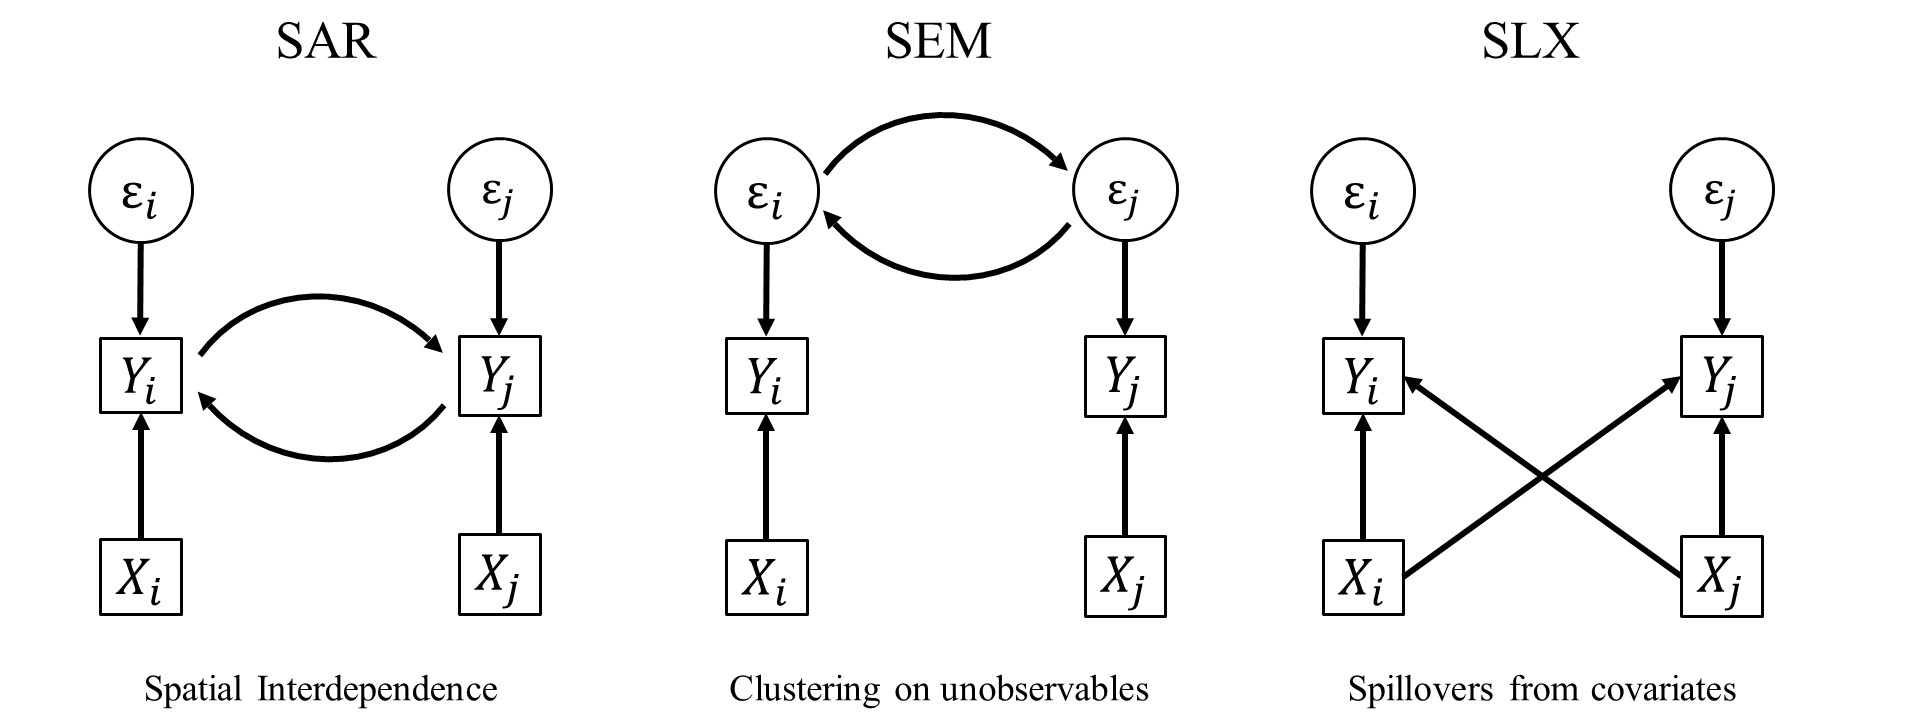
\includegraphics{fig/Graph.jpg}

Strictly speaking, there are some other possibilities too, such as
measurement error or the wrong choice on the spatial level. For
instance, imagine we have a city-specific characteristic (e.g.~public
spending) allocated to neighbourhood units. Obviously, this will
introduce heavy autocorrelation on the neighbourhood level by
construction.

There are three basic ways of incorporating spatial dependence, which
then can be further combined. As before, the \(N \times N\) spatial
weights matrix \(\boldsymbol{\mathbf{W}}\) defines the spatial
relationship between units.

\hypertarget{spatial-error-model-sem}{%
\subsection{Spatial Error Model (SEM)}\label{spatial-error-model-sem}}

\begin{itemize}
\tightlist
\item
  Clustering on Unobservables
\end{itemize}

\[
        \begin{equation} 
        \begin{split}
        {\boldsymbol{\mathbf{y}}}&=\alpha{\boldsymbol{\mathbf{\iota}}}+{\boldsymbol{\mathbf{X}}}{\boldsymbol{\mathbf{\beta}}}+{\boldsymbol{\mathbf{u}}},\\
        {\boldsymbol{\mathbf{u}}}&=\lambda{\boldsymbol{\mathbf{W}}}{\boldsymbol{\mathbf{u}}}+{\boldsymbol{\mathbf{\varepsilon}}}
        \end{split} 
        \end{equation}
\]

\(\lambda\) denotes the strength of the spatial correlation in the
errors of the model: \emph{your errors influence my errors}.

\begin{itemize}
\tightlist
\item
  \(> 0\): positive error dependence,
\item
  \(< 0\): negative error dependence,
\item
  \(= 0\): traditional OLS model.
\end{itemize}

\(\lambda\) is defined in the range \([-1, +1]\).

\hypertarget{spatial-autoregressive-model-sar}{%
\subsection{Spatial Autoregressive Model
(SAR)}\label{spatial-autoregressive-model-sar}}

\begin{itemize}
\tightlist
\item
  Interdependence
\end{itemize}

\[
    \begin{equation} 
        {\boldsymbol{\mathbf{y}}}=\alpha{\boldsymbol{\mathbf{\iota}}}+\rho{\boldsymbol{\mathbf{W}}}{\boldsymbol{\mathbf{y}}}+{\boldsymbol{\mathbf{X}}}{\boldsymbol{\mathbf{\beta}}}+ {\boldsymbol{\mathbf{\varepsilon}}}
        \end{equation}  
\]

\(\rho\) denotes the strength of the spatial correlation in the
dependent variable (spatial autocorrelation): \emph{your outcome
influences my outcome}.

\begin{itemize}
\tightlist
\item
  \(> 0\): positive spatial dependence,
\item
  \(< 0\): negative spatial dependence,
\item
  \(= 0\): traditional OLS model.
\end{itemize}

\(\rho\) is defined in the range \([-1, +1]\).

\hypertarget{spatially-lagged-x-model-slx}{%
\subsection{Spatially lagged X Model
(SLX)}\label{spatially-lagged-x-model-slx}}

\begin{itemize}
\tightlist
\item
  Spillovers in Covariates
\end{itemize}

\[
        \begin{equation}
        {\boldsymbol{\mathbf{y}}}=\alpha{\boldsymbol{\mathbf{\iota}}}+{\boldsymbol{\mathbf{X}}}{\boldsymbol{\mathbf{\beta}}}+{\boldsymbol{\mathbf{W}}}{\boldsymbol{\mathbf{X}}}{\boldsymbol{\mathbf{\theta}}}+ {\boldsymbol{\mathbf{\varepsilon}}}
        \end{equation}
\]

\(\theta\) denotes the strength of the spatial spillover effects from
covariate(s) on the dependent variable: \emph{your covariates influence
my outcome}.

\(\theta\) is basically like any other coefficient from a covariate. It
is thus not bound to any range.

Moreover, there are models combining two sets of the above
specifications.

\hypertarget{spatial-durbin-model-sdm}{%
\subsection{Spatial Durbin Model (SDM)}\label{spatial-durbin-model-sdm}}

\begin{itemize}
\tightlist
\item
  Interdependence
\item
  Spillovers in Covariates
\end{itemize}

\[
        \begin{equation}
        {\boldsymbol{\mathbf{y}}}=\alpha{\boldsymbol{\mathbf{\iota}}}+\rho{\boldsymbol{\mathbf{W}}}{\boldsymbol{\mathbf{y}}}+{\boldsymbol{\mathbf{X}}}{\boldsymbol{\mathbf{\beta}}}+{\boldsymbol{\mathbf{W}}}{\boldsymbol{\mathbf{X}}}{\boldsymbol{\mathbf{\theta}}}+ {\boldsymbol{\mathbf{\varepsilon}}}
        \end{equation}
\]

\hypertarget{spatial-durbin-error-model-sdem}{%
\subsection{Spatial Durbin Error Model
(SDEM)}\label{spatial-durbin-error-model-sdem}}

\begin{itemize}
\tightlist
\item
  Clustering on Unobservables
\item
  Spillovers in Covariates
\end{itemize}

\[
    \begin{equation}
        \begin{split}
        {\boldsymbol{\mathbf{y}}}&=\alpha{\boldsymbol{\mathbf{\iota}}}+{\boldsymbol{\mathbf{X}}}{\boldsymbol{\mathbf{\beta}}}+{\boldsymbol{\mathbf{W}}}{\boldsymbol{\mathbf{X}}}{\boldsymbol{\mathbf{\theta}}}+ {\boldsymbol{\mathbf{u}}},\\
        {\boldsymbol{\mathbf{u}}}&=\lambda{\boldsymbol{\mathbf{W}}}{\boldsymbol{\mathbf{u}}}+{\boldsymbol{\mathbf{\varepsilon}}}
        \end{split}
        \end{equation}
\]

\hypertarget{combined-spatial-autocorrelation-model-sac}{%
\subsection{Combined Spatial Autocorrelation Model
(SAC)}\label{combined-spatial-autocorrelation-model-sac}}

\begin{itemize}
\tightlist
\item
  Clustering on Unobservables
\item
  Interdependence
\end{itemize}

\[
        \begin{equation}
        \begin{split}
        {\boldsymbol{\mathbf{y}}}&=\alpha{\boldsymbol{\mathbf{\iota}}}+\rho{\boldsymbol{\mathbf{W}}}{\boldsymbol{\mathbf{y}}}+{\boldsymbol{\mathbf{X}}}{\boldsymbol{\mathbf{\beta}}}+ {\boldsymbol{\mathbf{u}}},\\
        {\boldsymbol{\mathbf{u}}}&=\lambda{\boldsymbol{\mathbf{W}}}{\boldsymbol{\mathbf{u}}}+{\boldsymbol{\mathbf{\varepsilon}}}
        \end{split}
        \end{equation}
\]

\hypertarget{general-nesting-spatial-model-gns}{%
\subsection{General Nesting Spatial Model
(GNS)}\label{general-nesting-spatial-model-gns}}

\begin{itemize}
\tightlist
\item
  Clustering on Unobservables
\item
  Interdependence
\item
  Spillovers in Covariates
\end{itemize}

\[
        \begin{equation}
        \begin{split}
        {\boldsymbol{\mathbf{y}}}&=\alpha{\boldsymbol{\mathbf{\iota}}}+\rho{\boldsymbol{\mathbf{W}}}{\boldsymbol{\mathbf{y}}}+{\boldsymbol{\mathbf{X}}}{\boldsymbol{\mathbf{\beta}}}+{\boldsymbol{\mathbf{W}}}{\boldsymbol{\mathbf{X}}}{\boldsymbol{\mathbf{\theta}}}+ {\boldsymbol{\mathbf{u}}},\\
        {\boldsymbol{\mathbf{u}}}&=\lambda{\boldsymbol{\mathbf{W}}}{\boldsymbol{\mathbf{u}}}+{\boldsymbol{\mathbf{\varepsilon}}}
        \end{split}
        \end{equation}
\]

\begin{tcolorbox}[enhanced jigsaw, opacitybacktitle=0.6, left=2mm, leftrule=.75mm, toptitle=1mm, breakable, colback=white, bottomrule=.15mm, colframe=quarto-callout-tip-color-frame, colbacktitle=quarto-callout-tip-color!10!white, coltitle=black, bottomtitle=1mm, titlerule=0mm, title=\textcolor{quarto-callout-tip-color}{\faLightbulb}\hspace{0.5em}{Manski's reflection problem}, opacityback=0, arc=.35mm, rightrule=.15mm, toprule=.15mm]

The General Nesting Spatial Model (GNS) is only weakly (or not?)
identifiable (Gibbons and Overman 2012).

It's analogous to Manski's reflection problem on neighbourhood effects
\citep{Manski.1993.0}: If people in the same group behave similar, this
can be because a) imitating behaviour of the group, b) exogenous
characteristics of the group influence the behaviour, and c) members of
the same group are exposed to the same external circumstances. \emph{We
just cannot separate those in observational data.}

\end{tcolorbox}

Note that all of these models assume different data generating processes
(DGP) leading to the spatial pattern. Although there are specifications
tests, it is generally not possible to let the data decide which one is
the true underlying DGP (Cook, Hays, and Franzese 2020; Rüttenauer
2022). However, there might be theoretical reasons to guide the model
specification (Cook, Hays, and Franzese 2020).

Just because SAR is probably the most commonly used model does not make
it the best choice. In contrast, various studies (Halleck Vega and
Elhorst 2015; Rüttenauer 2022; Wimpy, Whitten, and Williams 2021)
highlight the advantages of the relative simple SLX model. Moreover,
this specification can basically be incorporated in any other
statistical method.

\hypertarget{a-note-on-missings}{%
\subsection{A note on missings}\label{a-note-on-missings}}

Missing values create a problem in spatial data analysis. For instance,
in a local spillover model with an average of 10 neighbours, two initial
missing values will lead to 20 missing values in the spatially lagged
variable. For global spillover models, one initial missing will `flow'
through the neighbourhood system until the cutoff point (and create an
excess amount of missings).

Depending on the data, units with missings can either be dropped and
omitted from the initial weights creation, or we need to impute the data
first, e.g.~using interpolation or Kriging.

\hypertarget{mini-example}{%
\section{Mini Example}\label{mini-example}}

Let's try to make sense of this. We rely on a mini example using a few
units in Camden

\begin{Shaded}
\begin{Highlighting}[]
\NormalTok{sub.spdf }\OtherTok{\textless{}{-}}\NormalTok{ msoa.spdf[}\FunctionTok{c}\NormalTok{(}\DecValTok{172}\NormalTok{, }\DecValTok{175}\NormalTok{, }\DecValTok{178}\NormalTok{, }\DecValTok{179}\NormalTok{, }\DecValTok{181}\NormalTok{, }\DecValTok{182}\NormalTok{), ]}
\FunctionTok{mapview}\NormalTok{(sub.spdf)}
\end{Highlighting}
\end{Shaded}

\begin{figure}[H]

{\centering 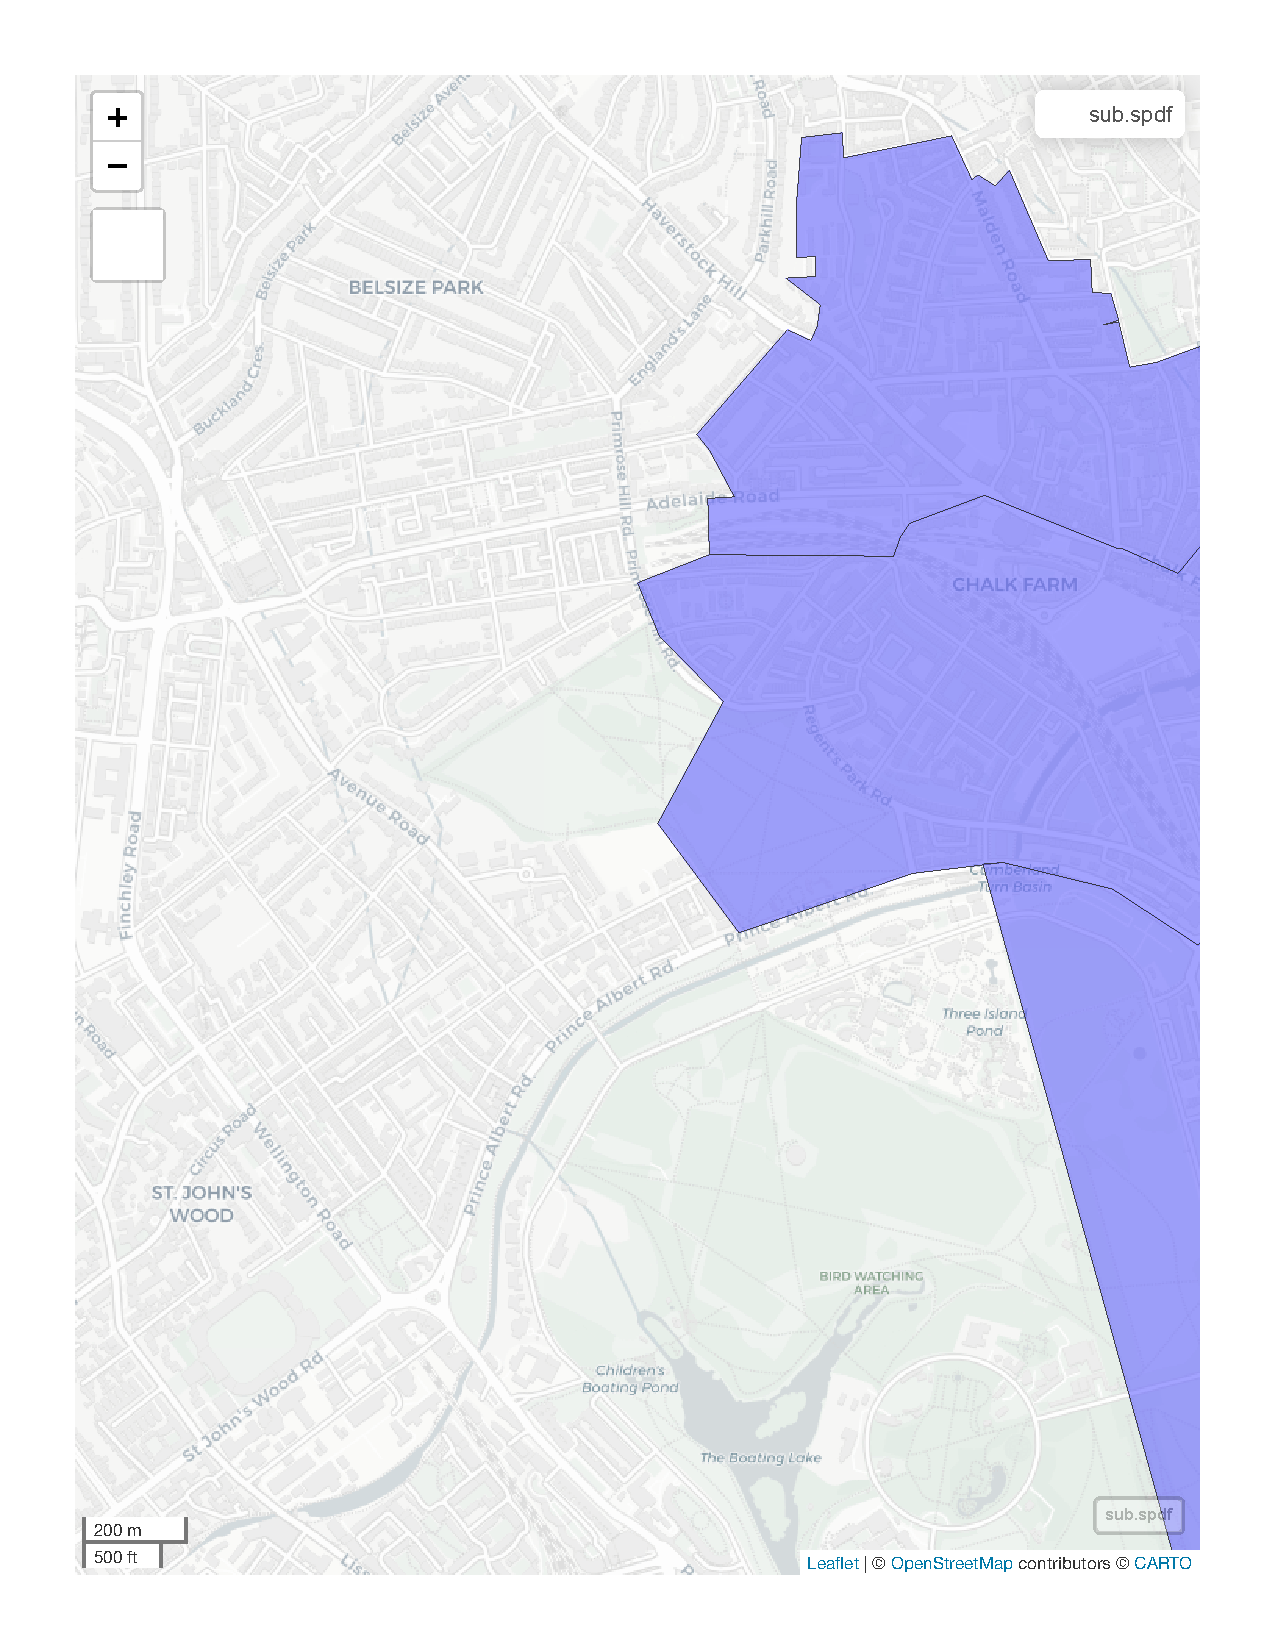
\includegraphics{05_regression-theory_files/figure-pdf/unnamed-chunk-4-1.pdf}

}

\end{figure}

We then construct queens neighbours, and have a look at the resulting
non-normalized matrix \(\boldsymbol{\mathbf{W}}\).

\begin{Shaded}
\begin{Highlighting}[]
\NormalTok{queens.nb }\OtherTok{\textless{}{-}} \FunctionTok{poly2nb}\NormalTok{(sub.spdf, }\AttributeTok{queen =} \ConstantTok{TRUE}\NormalTok{, }\AttributeTok{snap =} \DecValTok{1}\NormalTok{)}
\NormalTok{W }\OtherTok{\textless{}{-}} \FunctionTok{nb2mat}\NormalTok{(queens.nb, }\AttributeTok{style =} \StringTok{"B"}\NormalTok{)}
\NormalTok{W}
\end{Highlighting}
\end{Shaded}

\begin{verbatim}
    [,1] [,2] [,3] [,4] [,5] [,6]
172    0    0    1    0    0    0
175    0    0    0    1    0    1
178    1    0    0    1    1    0
179    0    1    1    0    1    1
181    0    0    1    1    0    1
182    0    1    0    1    1    0
attr(,"call")
nb2mat(neighbours = queens.nb, style = "B")
\end{verbatim}

We have selected 6 units. So, \(\boldsymbol{\mathbf{W}}\) is a
\(6 \times 6\) matrix. we see that observation 1 has one neighbour:
observation 3. Observation 2 has two nieghbours: observation 4 and
observation 6. The diagonal is zero: no unit is a neighbour of
themselves.

No we row-normalize this matrix.

\begin{Shaded}
\begin{Highlighting}[]
\NormalTok{queens.lw }\OtherTok{\textless{}{-}} \FunctionTok{nb2listw}\NormalTok{(queens.nb,}
                      \AttributeTok{style =} \StringTok{"W"}\NormalTok{)}
\NormalTok{W\_rn }\OtherTok{\textless{}{-}} \FunctionTok{listw2mat}\NormalTok{(queens.lw)}
\NormalTok{W\_rn}
\end{Highlighting}
\end{Shaded}

\begin{verbatim}
         [,1]      [,2]      [,3]      [,4]      [,5]      [,6]
172 0.0000000 0.0000000 1.0000000 0.0000000 0.0000000 0.0000000
175 0.0000000 0.0000000 0.0000000 0.5000000 0.0000000 0.5000000
178 0.3333333 0.0000000 0.0000000 0.3333333 0.3333333 0.0000000
179 0.0000000 0.2500000 0.2500000 0.0000000 0.2500000 0.2500000
181 0.0000000 0.0000000 0.3333333 0.3333333 0.0000000 0.3333333
182 0.0000000 0.3333333 0.0000000 0.3333333 0.3333333 0.0000000
\end{verbatim}

No every single weight \(w_{ij}\) is divided by the total number of
neighbours \(n_i\) of the focal unit. For observation 1, observation 3
is the only neighbour, thus a weight = 1. FOr observation two, both
neighbours have a weight of 1/2. For obervation 3 (with three
neighbours) each neighbour got a weight of 1/3.

\begin{tcolorbox}[enhanced jigsaw, opacitybacktitle=0.6, left=2mm, leftrule=.75mm, toptitle=1mm, breakable, colback=white, bottomrule=.15mm, colframe=quarto-callout-tip-color-frame, colbacktitle=quarto-callout-tip-color!10!white, coltitle=black, bottomtitle=1mm, titlerule=0mm, title=\textcolor{quarto-callout-tip-color}{\faLightbulb}\hspace{0.5em}{Question}, opacityback=0, arc=.35mm, rightrule=.15mm, toprule=.15mm]

What happens if we multiply this matrix \(\boldsymbol{\mathbf{W}}\) with
a \(N \times 1\) vector \(\boldsymbol{\mathbf{y}}\) or
\(\boldsymbol{\mathbf{x}}\)?

\end{tcolorbox}

A short reminder on matrix multiplication.

\[
\boldsymbol{\mathbf{W}} * \boldsymbol{\mathbf{y}} =
\begin{bmatrix}
w_{11} & w_{12} & w_{13}\\
w_{21} & w_{22} & w_{23}\\
w_{31} & w_{32} & w_{33} 
\end{bmatrix} *
\begin{bmatrix}
y_{11} \\
y_{21} \\
y_{31}  
\end{bmatrix}\\
= \begin{bmatrix}
w_{11}y_{11} + w_{12}y_{21} + w_{13}y_{31}\\
w_{21}y_{11} + w_{22}y_{21} + w_{23}y_{31}\\
w_{31}y_{11} + w_{32}y_{21} + w_{33}y_{31}  
\end{bmatrix}
\]

Each line of \(\boldsymbol{\mathbf{W}} * \boldsymbol{\mathbf{y}}\) just
gives a weighted average of the other \(y\)-values \(y_j\) in the
sample. In case of the row-normalization, each neighbour gets the same
weight \(\frac{1}{n_i}\). This is simply the mean of \(y_j\) of the
neighbours in case of a row-normalized contiguity weights matrix.

Note that the \emph{mean} interpretation is only valid with
row-normalization. What would we get with inverse-distance based
weights?

Let's look at this in our example

\begin{Shaded}
\begin{Highlighting}[]
\NormalTok{y }\OtherTok{\textless{}{-}}\NormalTok{ sub.spdf}\SpecialCharTok{$}\NormalTok{med\_house\_price}
\NormalTok{x }\OtherTok{\textless{}{-}}\NormalTok{ sub.spdf}\SpecialCharTok{$}\NormalTok{pubs\_count}

\NormalTok{W\_rn}
\end{Highlighting}
\end{Shaded}

\begin{verbatim}
         [,1]      [,2]      [,3]      [,4]      [,5]      [,6]
172 0.0000000 0.0000000 1.0000000 0.0000000 0.0000000 0.0000000
175 0.0000000 0.0000000 0.0000000 0.5000000 0.0000000 0.5000000
178 0.3333333 0.0000000 0.0000000 0.3333333 0.3333333 0.0000000
179 0.0000000 0.2500000 0.2500000 0.0000000 0.2500000 0.2500000
181 0.0000000 0.0000000 0.3333333 0.3333333 0.0000000 0.3333333
182 0.0000000 0.3333333 0.0000000 0.3333333 0.3333333 0.0000000
\end{verbatim}

\begin{Shaded}
\begin{Highlighting}[]
\NormalTok{y}
\end{Highlighting}
\end{Shaded}

\begin{verbatim}
[1] 376812.5 414625.0 713125.0 322750.0 495000.0 364000.0
\end{verbatim}

\begin{Shaded}
\begin{Highlighting}[]
\NormalTok{x}
\end{Highlighting}
\end{Shaded}

\begin{verbatim}
[1] 1 3 3 1 9 7
\end{verbatim}

\begin{Shaded}
\begin{Highlighting}[]
\NormalTok{W\_rn\_y }\OtherTok{\textless{}{-}}\NormalTok{ W\_rn }\SpecialCharTok{\%*\%}\NormalTok{ y}
\NormalTok{W\_rn\_x }\OtherTok{\textless{}{-}}\NormalTok{ W\_rn }\SpecialCharTok{\%*\%}\NormalTok{ x}
\NormalTok{W\_rn\_y}
\end{Highlighting}
\end{Shaded}

\begin{verbatim}
        [,1]
172 713125.0
175 343375.0
178 398187.5
179 496687.5
181 466625.0
182 410791.7
\end{verbatim}

\begin{Shaded}
\begin{Highlighting}[]
\NormalTok{W\_rn\_x}
\end{Highlighting}
\end{Shaded}

\begin{verbatim}
        [,1]
172 3.000000
175 4.000000
178 3.666667
179 5.500000
181 3.666667
182 4.333333
\end{verbatim}

Let's check if our interpretation is true

\begin{Shaded}
\begin{Highlighting}[]
\NormalTok{W\_rn\_y[}\DecValTok{1}\NormalTok{] }\SpecialCharTok{==}\NormalTok{ y[}\DecValTok{3}\NormalTok{]}
\end{Highlighting}
\end{Shaded}

\begin{verbatim}
[1] TRUE
\end{verbatim}

\begin{Shaded}
\begin{Highlighting}[]
\NormalTok{W\_rn\_y[}\DecValTok{2}\NormalTok{] }\SpecialCharTok{==} \FunctionTok{mean}\NormalTok{(y[}\FunctionTok{c}\NormalTok{(}\DecValTok{4}\NormalTok{, }\DecValTok{6}\NormalTok{)])}
\end{Highlighting}
\end{Shaded}

\begin{verbatim}
[1] TRUE
\end{verbatim}

\begin{Shaded}
\begin{Highlighting}[]
\NormalTok{W\_rn\_y[}\DecValTok{4}\NormalTok{] }\SpecialCharTok{==} \FunctionTok{mean}\NormalTok{(y[}\FunctionTok{c}\NormalTok{(}\DecValTok{2}\NormalTok{, }\DecValTok{3}\NormalTok{, }\DecValTok{5}\NormalTok{, }\DecValTok{6}\NormalTok{)])}
\end{Highlighting}
\end{Shaded}

\begin{verbatim}
[1] TRUE
\end{verbatim}

\hypertarget{real-example}{%
\section{Real Example}\label{real-example}}

First, we need the a spatial weights matrix.

\begin{Shaded}
\begin{Highlighting}[]
\CommentTok{\# Contiguity (Queens) neighbours weights}
\NormalTok{queens.nb }\OtherTok{\textless{}{-}} \FunctionTok{poly2nb}\NormalTok{(msoa.spdf, }
                     \AttributeTok{queen =} \ConstantTok{TRUE}\NormalTok{, }
                     \AttributeTok{snap =} \DecValTok{1}\NormalTok{) }\CommentTok{\# we consider points in 1m distance as \textquotesingle{}touching\textquotesingle{}}
\NormalTok{queens.lw }\OtherTok{\textless{}{-}} \FunctionTok{nb2listw}\NormalTok{(queens.nb,}
                      \AttributeTok{style =} \StringTok{"W"}\NormalTok{)}
\end{Highlighting}
\end{Shaded}

We can estimate spatial models using \texttt{spatialreg}.

\hypertarget{sar}{%
\subsection{SAR}\label{sar}}

Let's estimate a spatial SAR model using the \texttt{lagsarlm()} with
contiguity weights. We use median house value as depended variable, and
include population density (\texttt{POPDEN}), the air pollution
(\texttt{no2}), and the share of ethnic minorities (\texttt{per\_mixed},
\texttt{per\_asian}, \texttt{per\_black}, \texttt{per\_other}).

\begin{Shaded}
\begin{Highlighting}[]
\NormalTok{mod\_1.sar }\OtherTok{\textless{}{-}} \FunctionTok{lagsarlm}\NormalTok{(}\FunctionTok{log}\NormalTok{(med\_house\_price) }\SpecialCharTok{\textasciitilde{}} \FunctionTok{log}\NormalTok{(no2) }\SpecialCharTok{+} \FunctionTok{log}\NormalTok{(POPDEN) }\SpecialCharTok{+} 
\NormalTok{                        per\_mixed }\SpecialCharTok{+}\NormalTok{ per\_asian }\SpecialCharTok{+}\NormalTok{ per\_black }\SpecialCharTok{+}\NormalTok{ per\_other,  }
                      \AttributeTok{data =}\NormalTok{ msoa.spdf, }
                      \AttributeTok{listw =}\NormalTok{ queens.lw,}
                      \AttributeTok{Durbin =} \ConstantTok{FALSE}\NormalTok{) }\CommentTok{\# we could here extend to SDM}
\FunctionTok{summary}\NormalTok{(mod\_1.sar)}
\end{Highlighting}
\end{Shaded}

\begin{verbatim}

Call:lagsarlm(formula = log(med_house_price) ~ log(no2) + log(POPDEN) + 
    per_mixed + per_asian + per_black + per_other, data = msoa.spdf, 
    listw = queens.lw, Durbin = FALSE)

Residuals:
       Min         1Q     Median         3Q        Max 
-0.5281789 -0.1220524 -0.0099245  0.0992203  1.0936745 

Type: lag 
Coefficients: (asymptotic standard errors) 
               Estimate  Std. Error  z value  Pr(>|z|)
(Intercept)  3.17383180  0.29041604  10.9286 < 2.2e-16
log(no2)     0.39705423  0.04452880   8.9168 < 2.2e-16
log(POPDEN) -0.05583014  0.01242876  -4.4920 7.055e-06
per_mixed    0.01851577  0.00579832   3.1933  0.001407
per_asian   -0.00228346  0.00045876  -4.9775 6.442e-07
per_black   -0.01263650  0.00100282 -12.6009 < 2.2e-16
per_other   -0.00161419  0.00289082  -0.5584  0.576582

Rho: 0.66976, LR test value: 473.23, p-value: < 2.22e-16
Asymptotic standard error: 0.025311
    z-value: 26.461, p-value: < 2.22e-16
Wald statistic: 700.19, p-value: < 2.22e-16

Log likelihood: 196.7203 for lag model
ML residual variance (sigma squared): 0.035402, (sigma: 0.18815)
Number of observations: 983 
Number of parameters estimated: 9 
AIC: -375.44, (AIC for lm: 95.786)
LM test for residual autocorrelation
test value: 8.609, p-value: 0.0033451
\end{verbatim}

This looks pretty much like a conventional model output, with some
additional information: a highly significant \texttt{mod\_1.sar\$rho} of
0.67 indicates strong positive spatial autocorrelation.

Remember that is the coefficient for the term
\(\boldsymbol{\mathbf{y}} = \rho \boldsymbol{\mathbf{W}} \boldsymbol{\mathbf{y}} \ldots\).
It is bound to be below 1 for positive autocorrelation.

In substantive terms, house prices in the focal unit positively
influence house prices in neighbouring units, which again influences
house prices among the neighbours of these neighbours, and so on (we'll
get back to this).

\begin{tcolorbox}[enhanced jigsaw, opacitybacktitle=0.6, left=2mm, leftrule=.75mm, toptitle=1mm, breakable, colback=white, bottomrule=.15mm, colframe=quarto-callout-warning-color-frame, colbacktitle=quarto-callout-warning-color!10!white, coltitle=black, bottomtitle=1mm, titlerule=0mm, title=\textcolor{quarto-callout-warning-color}{\faExclamationTriangle}\hspace{0.5em}{Warning}, opacityback=0, arc=.35mm, rightrule=.15mm, toprule=.15mm]

The coefficients of covariates in a SAR model are not marginal or
partical effects, because of the spillovers and feedback loops in
\(\boldsymbol{\mathbf{y}}\) (see below)!

From the coefficient, we can only interpret the direction: there's a
positive effect of air pollution and a negative effect of population
sensity, and so on\ldots{}

\end{tcolorbox}

\hypertarget{sem}{%
\subsection{SEM}\label{sem}}

SEM models can be estimated using \texttt{errorsarlm()}.

\begin{Shaded}
\begin{Highlighting}[]
\NormalTok{mod\_1.sem }\OtherTok{\textless{}{-}} \FunctionTok{errorsarlm}\NormalTok{(}\FunctionTok{log}\NormalTok{(med\_house\_price) }\SpecialCharTok{\textasciitilde{}} \FunctionTok{log}\NormalTok{(no2) }\SpecialCharTok{+} \FunctionTok{log}\NormalTok{(POPDEN) }\SpecialCharTok{+}
\NormalTok{                          per\_mixed }\SpecialCharTok{+}\NormalTok{ per\_asian }\SpecialCharTok{+}\NormalTok{ per\_black }\SpecialCharTok{+}\NormalTok{ per\_other,  }
                        \AttributeTok{data =}\NormalTok{ msoa.spdf, }
                        \AttributeTok{listw =}\NormalTok{ queens.lw,}
                        \AttributeTok{Durbin =} \ConstantTok{FALSE}\NormalTok{) }\CommentTok{\# we could here extend to SDEM}
\FunctionTok{summary}\NormalTok{(mod\_1.sem)}
\end{Highlighting}
\end{Shaded}

\begin{verbatim}

Call:errorsarlm(formula = log(med_house_price) ~ log(no2) + log(POPDEN) + 
    per_mixed + per_asian + per_black + per_other, data = msoa.spdf, 
    listw = queens.lw, Durbin = FALSE)

Residuals:
      Min        1Q    Median        3Q       Max 
-0.581785 -0.105218 -0.012758  0.094430  0.913425 

Type: error 
Coefficients: (asymptotic standard errors) 
               Estimate  Std. Error  z value  Pr(>|z|)
(Intercept) 12.92801104  0.35239139  36.6865 < 2.2e-16
log(no2)     0.15735296  0.10880727   1.4462 0.1481317
log(POPDEN) -0.08316270  0.01254315  -6.6301 3.354e-11
per_mixed   -0.03377962  0.00811054  -4.1649 3.115e-05
per_asian   -0.00413115  0.00096849  -4.2656 1.994e-05
per_black   -0.01653816  0.00126741 -13.0488 < 2.2e-16
per_other   -0.01693012  0.00462999  -3.6566 0.0002556

Lambda: 0.88605, LR test value: 623.55, p-value: < 2.22e-16
Asymptotic standard error: 0.015803
    z-value: 56.068, p-value: < 2.22e-16
Wald statistic: 3143.6, p-value: < 2.22e-16

Log likelihood: 271.8839 for error model
ML residual variance (sigma squared): 0.026911, (sigma: 0.16405)
Number of observations: 983 
Number of parameters estimated: 9 
AIC: -525.77, (AIC for lm: 95.786)
\end{verbatim}

In this case \texttt{mod\_1.sem\$lambda} gives us the spatial parameter.
A highly significant lambda of 0.89 indicates that the errors are highly
spatially correlated (e.g.~due to correlated unobservables). Again,
\$\lambda = 1 \$ would be the maximum.

In spatial error models, we can interpret the coefficients directly, as
in a conventional linear model.

\hypertarget{slx}{%
\subsection{SLX}\label{slx}}

SLX models can either be estimated with \texttt{lmSLX()} directly, or by
creating \(\boldsymbol{\mathbf{W}} \boldsymbol{\mathbf{X}}\) manually
and plugging it into any available model-fitting function.

\begin{Shaded}
\begin{Highlighting}[]
\NormalTok{mod\_1.slx }\OtherTok{\textless{}{-}} \FunctionTok{lmSLX}\NormalTok{(}\FunctionTok{log}\NormalTok{(med\_house\_price) }\SpecialCharTok{\textasciitilde{}} \FunctionTok{log}\NormalTok{(no2) }\SpecialCharTok{+} \FunctionTok{log}\NormalTok{(POPDEN) }\SpecialCharTok{+} 
\NormalTok{                     per\_mixed }\SpecialCharTok{+}\NormalTok{ per\_asian }\SpecialCharTok{+}\NormalTok{ per\_black }\SpecialCharTok{+}\NormalTok{ per\_other,  }
                   \AttributeTok{data =}\NormalTok{ msoa.spdf, }
                   \AttributeTok{listw =}\NormalTok{ queens.lw, }
                   \AttributeTok{Durbin =} \ConstantTok{TRUE}\NormalTok{) }\CommentTok{\# use a formula to lag only specific covariates}
\FunctionTok{summary}\NormalTok{(mod\_1.slx)}
\end{Highlighting}
\end{Shaded}

\begin{verbatim}

Call:
lm(formula = formula(paste("y ~ ", paste(colnames(x)[-1], collapse = "+"))), 
    data = as.data.frame(x), weights = weights)

Coefficients:
                 Estimate    Std. Error  t value     Pr(>|t|)  
(Intercept)       1.058e+01   1.539e-01   6.878e+01   0.000e+00
log.no2.         -4.407e-01   1.811e-01  -2.434e+00   1.511e-02
log.POPDEN.      -7.684e-02   1.734e-02  -4.430e+00   1.049e-05
per_mixed        -3.304e-02   1.130e-02  -2.925e+00   3.530e-03
per_asian        -2.381e-03   1.474e-03  -1.615e+00   1.065e-01
per_black        -1.623e-02   1.801e-03  -9.009e+00   1.080e-18
per_other        -2.039e-02   6.564e-03  -3.107e+00   1.947e-03
lag.log.no2.      9.936e-01   1.994e-01   4.984e+00   7.384e-07
lag.log.POPDEN.   1.133e-01   2.875e-02   3.939e+00   8.759e-05
lag.per_mixed     1.261e-01   1.429e-02   8.820e+00   5.249e-18
lag.per_asian    -3.828e-03   1.661e-03  -2.305e+00   2.140e-02
lag.per_black    -1.805e-02   2.241e-03  -8.056e+00   2.296e-15
lag.per_other     4.814e-02   7.971e-03   6.039e+00   2.204e-09
\end{verbatim}

In SLX models, we can simply interpret the coefficients of direct and
indirect (spatially lagged) covariates.

For instance, lets look at population density:

\begin{tcolorbox}[enhanced jigsaw, opacitybacktitle=0.6, left=2mm, leftrule=.75mm, toptitle=1mm, breakable, colback=white, bottomrule=.15mm, colframe=quarto-callout-tip-color-frame, colbacktitle=quarto-callout-tip-color!10!white, coltitle=black, bottomtitle=1mm, titlerule=0mm, title=\textcolor{quarto-callout-tip-color}{\faLightbulb}\hspace{0.5em}{Interpretaion SLX}, opacityback=0, arc=.35mm, rightrule=.15mm, toprule=.15mm]

\begin{enumerate}
\def\labelenumi{\arabic{enumi}.}
\item
  A high population density in the focal unit is related to lower house
  prices (a 1\% increase in population density decreses house prices by
  -0.08\%), but
\item
  A high population density in the neighbouring areas is related to
  higher house prices (while keeping population density in the focal
  unit constant). A 1\% increase in the \emph{average} population
  density \emph{across the adjacent neighbourhoods} increases house
  prices in \emph{the focal unit} by 0.11\%)
\end{enumerate}

Potential interpretation: areas with a low population density in central
regions of the city (high pop density in surrounding neighbourhoods)
have higher house prices. We could try testing this interpretation by
including the distance to the city centre as a control.

\end{tcolorbox}

Also note how the air pollution coefficient has changed here, with a
negative effect in the focal unit and positive one among the
neighbouring units.

An alternative way of estimating the same model is lagging the
covariates first.

\begin{Shaded}
\begin{Highlighting}[]
\CommentTok{\# Loop through vars and create lagged variables}
\NormalTok{msoa.spdf}\SpecialCharTok{$}\NormalTok{log\_POPDEN }\OtherTok{\textless{}{-}} \FunctionTok{log}\NormalTok{(msoa.spdf}\SpecialCharTok{$}\NormalTok{POPDEN)}
\NormalTok{msoa.spdf}\SpecialCharTok{$}\NormalTok{log\_no2 }\OtherTok{\textless{}{-}} \FunctionTok{log}\NormalTok{(msoa.spdf}\SpecialCharTok{$}\NormalTok{no2)}
\NormalTok{msoa.spdf}\SpecialCharTok{$}\NormalTok{log\_med\_house\_price }\OtherTok{\textless{}{-}} \FunctionTok{log}\NormalTok{(msoa.spdf}\SpecialCharTok{$}\NormalTok{med\_house\_price)}

\NormalTok{vars }\OtherTok{\textless{}{-}} \FunctionTok{c}\NormalTok{(}\StringTok{"log\_med\_house\_price"}\NormalTok{, }\StringTok{"log\_no2"}\NormalTok{, }\StringTok{"log\_POPDEN"}\NormalTok{, }
          \StringTok{"per\_mixed"}\NormalTok{, }\StringTok{"per\_asian"}\NormalTok{, }\StringTok{"per\_black"}\NormalTok{, }\StringTok{"per\_other"}\NormalTok{,}
          \StringTok{"per\_owner"}\NormalTok{, }\StringTok{"per\_social"}\NormalTok{, }\StringTok{"pubs\_count"}\NormalTok{)}
\ControlFlowTok{for}\NormalTok{(v }\ControlFlowTok{in}\NormalTok{ vars)\{}
\NormalTok{  msoa.spdf[, }\FunctionTok{paste0}\NormalTok{(}\StringTok{"w."}\NormalTok{, v)] }\OtherTok{\textless{}{-}} \FunctionTok{lag.listw}\NormalTok{(queens.lw,}
                                            \AttributeTok{var =} \FunctionTok{st\_drop\_geometry}\NormalTok{(msoa.spdf)[, v])}
\NormalTok{\}}

\CommentTok{\# Alternatively:}
\NormalTok{w\_vars }\OtherTok{\textless{}{-}} \FunctionTok{create\_WX}\NormalTok{(}\FunctionTok{st\_drop\_geometry}\NormalTok{(msoa.spdf[, vars]),}
                    \AttributeTok{listw =}\NormalTok{ queens.lw,}
                    \AttributeTok{prefix =} \StringTok{"w"}\NormalTok{)}

\FunctionTok{head}\NormalTok{(w\_vars)}
\end{Highlighting}
\end{Shaded}

\begin{verbatim}
  w.log_med_house_price w.log_no2 w.log_POPDEN w.per_mixed w.per_asian
1              12.98382  3.843750     4.662014    4.748368   23.899916
2              12.28730  3.098960     3.300901    3.978275   19.951593
3              12.21207  3.206338     4.009795    3.997487   20.793559
4              12.18176  3.169934     3.630360    2.759082    7.633439
5              12.11159  3.221203     3.993660    3.930061   12.791140
6              12.08393  3.217865     3.876070    3.419488    8.997514
  w.per_black w.per_other w.per_owner w.per_social w.pubs_count
1    7.879758   3.2080074    25.75738     33.85580    8.5454545
2   10.451828   1.6368986    66.42278     15.75042    0.6666667
3   12.965863   1.7526693    58.72637     21.38169    0.2857143
4   12.135478   0.6992118    66.52519     19.70500    0.2000000
5   16.108948   1.3817357    53.05539     29.44022    0.4000000
6   15.312652   0.9611710    59.49460     23.81126    0.1666667
\end{verbatim}

And subsequently we use those new variables in a linear model.

\begin{Shaded}
\begin{Highlighting}[]
\NormalTok{mod\_1.lm }\OtherTok{\textless{}{-}} \FunctionTok{lm}\NormalTok{ (}\FunctionTok{log}\NormalTok{(med\_house\_price) }\SpecialCharTok{\textasciitilde{}} \FunctionTok{log}\NormalTok{(no2) }\SpecialCharTok{+} \FunctionTok{log}\NormalTok{(POPDEN) }\SpecialCharTok{+} 
\NormalTok{                  per\_mixed }\SpecialCharTok{+}\NormalTok{ per\_asian }\SpecialCharTok{+}\NormalTok{ per\_black }\SpecialCharTok{+}\NormalTok{ per\_other }\SpecialCharTok{+}
\NormalTok{                  w.log\_no2 }\SpecialCharTok{+}\NormalTok{ w.log\_POPDEN }\SpecialCharTok{+}
\NormalTok{                  w.per\_mixed }\SpecialCharTok{+}\NormalTok{ w.per\_asian }\SpecialCharTok{+}\NormalTok{ w.per\_black }\SpecialCharTok{+}\NormalTok{ w.per\_other,}
                \AttributeTok{data =}\NormalTok{ msoa.spdf)}
\FunctionTok{summary}\NormalTok{(mod\_1.lm)}
\end{Highlighting}
\end{Shaded}

\begin{verbatim}

Call:
lm(formula = log(med_house_price) ~ log(no2) + log(POPDEN) + 
    per_mixed + per_asian + per_black + per_other + w.log_no2 + 
    w.log_POPDEN + w.per_mixed + w.per_asian + w.per_black + 
    w.per_other, data = msoa.spdf)

Residuals:
     Min       1Q   Median       3Q      Max 
-0.50809 -0.16605 -0.01817  0.13055  1.09039 

Coefficients:
              Estimate Std. Error t value Pr(>|t|)    
(Intercept)  10.582440   0.153862  68.779  < 2e-16 ***
log(no2)     -0.440727   0.181063  -2.434  0.01511 *  
log(POPDEN)  -0.076840   0.017345  -4.430 1.05e-05 ***
per_mixed    -0.033042   0.011298  -2.925  0.00353 ** 
per_asian    -0.002381   0.001474  -1.615  0.10655    
per_black    -0.016229   0.001801  -9.009  < 2e-16 ***
per_other    -0.020391   0.006564  -3.107  0.00195 ** 
w.log_no2     0.993602   0.199370   4.984 7.38e-07 ***
w.log_POPDEN  0.113262   0.028752   3.939 8.76e-05 ***
w.per_mixed   0.126069   0.014294   8.820  < 2e-16 ***
w.per_asian  -0.003828   0.001661  -2.305  0.02140 *  
w.per_black  -0.018054   0.002241  -8.056 2.30e-15 ***
w.per_other   0.048139   0.007971   6.039 2.20e-09 ***
---
Signif. codes:  0 '***' 0.001 '**' 0.01 '*' 0.05 '.' 0.1 ' ' 1

Residual standard error: 0.2262 on 970 degrees of freedom
Multiple R-squared:  0.653, Adjusted R-squared:  0.6487 
F-statistic: 152.1 on 12 and 970 DF,  p-value: < 2.2e-16
\end{verbatim}

Looks pretty similar to \texttt{lmSLX()} results, and it should! A big
advantage of the SLX specification is that we can use the lagged
variables in basically all methods which take variables as inputs, such
as non-linear models, matching algorithms, and machine learning tools.

Moreover, using the lagged variables gives a high degree of freedom. For
instance, we could (not saying that it necessarily makes sense):

\begin{itemize}
\item
  Use different weights matrices for different variables
\item
  Include higher order neighbours using \texttt{nblag()} (with an
  increasing number of orders we go towards a more global model, but we
  estimate a coefficient for each spillover, instead of estimating just
  one)
\item
  Use machine learning techniques to determine the best fitting weights
  specification.
\end{itemize}

\hypertarget{sdem}{%
\subsection{SDEM}\label{sdem}}

SDEM models can be estimated using \texttt{errorsarlm()} with the
additional option \texttt{Durbin\ =\ TRUE}.

\begin{Shaded}
\begin{Highlighting}[]
\NormalTok{mod\_1.sdem }\OtherTok{\textless{}{-}} \FunctionTok{errorsarlm}\NormalTok{(}\FunctionTok{log}\NormalTok{(med\_house\_price) }\SpecialCharTok{\textasciitilde{}} \FunctionTok{log}\NormalTok{(no2) }\SpecialCharTok{+} \FunctionTok{log}\NormalTok{(POPDEN) }\SpecialCharTok{+}
\NormalTok{                          per\_mixed }\SpecialCharTok{+}\NormalTok{ per\_asian }\SpecialCharTok{+}\NormalTok{ per\_black }\SpecialCharTok{+}\NormalTok{ per\_other,  }
                        \AttributeTok{data =}\NormalTok{ msoa.spdf, }
                        \AttributeTok{listw =}\NormalTok{ queens.lw,}
                        \AttributeTok{Durbin =} \ConstantTok{TRUE}\NormalTok{) }\CommentTok{\# we could here extend to SDEM}
\FunctionTok{summary}\NormalTok{(mod\_1.sdem)}
\end{Highlighting}
\end{Shaded}

\begin{verbatim}

Call:errorsarlm(formula = log(med_house_price) ~ log(no2) + log(POPDEN) + 
    per_mixed + per_asian + per_black + per_other, data = msoa.spdf, 
    listw = queens.lw, Durbin = TRUE)

Residuals:
      Min        1Q    Median        3Q       Max 
-0.617795 -0.106380 -0.014832  0.095826  0.927446 

Type: error 
Coefficients: (asymptotic standard errors) 
                  Estimate Std. Error  z value  Pr(>|z|)
(Intercept)     10.4422703  0.3652148  28.5921 < 2.2e-16
log(no2)        -0.2057493  0.1264914  -1.6266 0.1038248
log(POPDEN)     -0.0769743  0.0132094  -5.8272 5.635e-09
per_mixed       -0.0222406  0.0079705  -2.7904 0.0052649
per_asian       -0.0037484  0.0010054  -3.7284 0.0001927
per_black       -0.0179751  0.0012383 -14.5161 < 2.2e-16
per_other       -0.0150218  0.0044895  -3.3460 0.0008199
lag.log(no2)     1.0004491  0.1739833   5.7503 8.911e-09
lag.log(POPDEN) -0.0054241  0.0327802  -0.1655 0.8685763
lag.per_mixed    0.0669699  0.0169349   3.9545 7.668e-05
lag.per_asian   -0.0018566  0.0015957  -1.1635 0.2446368
lag.per_black   -0.0079949  0.0024833  -3.2195 0.0012842
lag.per_other    0.0273378  0.0087430   3.1268 0.0017671

Lambda: 0.76173, LR test value: 455.7, p-value: < 2.22e-16
Asymptotic standard error: 0.024949
    z-value: 30.531, p-value: < 2.22e-16
Wald statistic: 932.15, p-value: < 2.22e-16

Log likelihood: 300.847 for error model
ML residual variance (sigma squared): 0.027504, (sigma: 0.16584)
Number of observations: 983 
Number of parameters estimated: 15 
AIC: -571.69, (AIC for lm: -117.99)
\end{verbatim}

And this SDEM can be interpreted like a combination of SEM and SLX.

First, we still see highly significant auto-correlation in the error
term. However, it's lower in magnitude now that we also include the
\(\boldsymbol{\mathbf{W}} X\) terms.

Second, the coefficients tell a similar story as in the SLX (use the
same interpretation), but some coefficient magnitudes have become
smaller.

\hypertarget{sdm}{%
\subsection{SDM}\label{sdm}}

SDM models can be estimated using \texttt{lagsarlm()} with the
additional option \texttt{Durbin\ =\ TRUE}.

\begin{Shaded}
\begin{Highlighting}[]
\NormalTok{mod\_1.sdm }\OtherTok{\textless{}{-}} \FunctionTok{lagsarlm}\NormalTok{(}\FunctionTok{log}\NormalTok{(med\_house\_price) }\SpecialCharTok{\textasciitilde{}} \FunctionTok{log}\NormalTok{(no2) }\SpecialCharTok{+} \FunctionTok{log}\NormalTok{(POPDEN) }\SpecialCharTok{+} 
\NormalTok{                        per\_mixed }\SpecialCharTok{+}\NormalTok{ per\_asian }\SpecialCharTok{+}\NormalTok{ per\_black }\SpecialCharTok{+}\NormalTok{ per\_other,  }
                      \AttributeTok{data =}\NormalTok{ msoa.spdf, }
                      \AttributeTok{listw =}\NormalTok{ queens.lw,}
                      \AttributeTok{Durbin =} \ConstantTok{TRUE}\NormalTok{) }\CommentTok{\# we could here extend to SDM}
\FunctionTok{summary}\NormalTok{(mod\_1.sdm)}
\end{Highlighting}
\end{Shaded}

\begin{verbatim}

Call:lagsarlm(formula = log(med_house_price) ~ log(no2) + log(POPDEN) + 
    per_mixed + per_asian + per_black + per_other, data = msoa.spdf, 
    listw = queens.lw, Durbin = TRUE)

Residuals:
      Min        1Q    Median        3Q       Max 
-0.614314 -0.107947 -0.013509  0.092234  0.917398 

Type: mixed 
Coefficients: (asymptotic standard errors) 
                  Estimate Std. Error  z value  Pr(>|z|)
(Intercept)      2.7843426  0.2944721   9.4554 < 2.2e-16
log(no2)        -0.3112762  0.1308101  -2.3796 0.0173312
log(POPDEN)     -0.0802866  0.0125213  -6.4120 1.436e-10
per_mixed       -0.0368998  0.0081596  -4.5223 6.118e-06
per_asian       -0.0033726  0.0010636  -3.1711 0.0015189
per_black       -0.0159770  0.0013006 -12.2848 < 2.2e-16
per_other       -0.0209743  0.0047369  -4.4279 9.516e-06
lag.log(no2)     0.4880923  0.1456778   3.3505 0.0008067
lag.log(POPDEN)  0.0781188  0.0207600   3.7629 0.0001679
lag.per_mixed    0.0640880  0.0104646   6.1243 9.110e-10
lag.per_asian    0.0017665  0.0012101   1.4598 0.1443498
lag.per_black    0.0070487  0.0017938   3.9295 8.511e-05
lag.per_other    0.0284822  0.0057774   4.9299 8.226e-07

Rho: 0.73126, LR test value: 501.83, p-value: < 2.22e-16
Asymptotic standard error: 0.025889
    z-value: 28.246, p-value: < 2.22e-16
Wald statistic: 797.86, p-value: < 2.22e-16

Log likelihood: 323.9111 for mixed model
ML residual variance (sigma squared): 0.026633, (sigma: 0.1632)
Number of observations: 983 
Number of parameters estimated: 15 
AIC: -617.82, (AIC for lm: -117.99)
LM test for residual autocorrelation
test value: 36.704, p-value: 1.3747e-09
\end{verbatim}

And this SDM can be interpreted like a combination of SAR and SLX.

First, there's still substantial auto-correlation in
\(\boldsymbol{\mathbf{y}}\), and this has become even stronger as
compared to SAR.

Second, we can interpret the direction of the effect, but we
\emph{cannot interpret the coefficient as marginal effects}.

\bookmarksetup{startatroot}

\hypertarget{spatial-regression-models-estimation}{%
\chapter{Spatial Regression Models:
Estimation}\label{spatial-regression-models-estimation}}

\newcommand{\Exp}{\mathrm{E}}
\newcommand\given[1][]{\:#1\vert\:}
\newcommand{\Cov}{\mathrm{Cov}}
\newcommand{\Var}{\mathrm{Var}}
\newcommand{\rank}{\mathrm{rank}}
\newcommand{\bm}[1]{\boldsymbol{\mathbf{#1}}}
\newcommand{\tr}{\mathrm{tr}}
\newcommand{\plim}{\operatornamewithlimits{plim}}
\newcommand{\diag}{\mathrm{diag}}

This section is strongly based on Sarrias (2023), despite being much
less detailed then the original.

\hypertarget{required-packages-6}{%
\subsection*{Required packages}\label{required-packages-6}}
\addcontentsline{toc}{subsection}{Required packages}

\begin{Shaded}
\begin{Highlighting}[]
\NormalTok{pkgs }\OtherTok{\textless{}{-}} \FunctionTok{c}\NormalTok{(}\StringTok{"sf"}\NormalTok{, }\StringTok{"mapview"}\NormalTok{, }\StringTok{"spdep"}\NormalTok{, }\StringTok{"spatialreg"}\NormalTok{, }\StringTok{"tmap"}\NormalTok{, }\StringTok{"viridisLite"}\NormalTok{) }\CommentTok{\# note: load spdep first, then spatialreg}
\FunctionTok{lapply}\NormalTok{(pkgs, require, }\AttributeTok{character.only =} \ConstantTok{TRUE}\NormalTok{)}
\end{Highlighting}
\end{Shaded}

\hypertarget{session-info-6}{%
\subsection*{Session info}\label{session-info-6}}
\addcontentsline{toc}{subsection}{Session info}

\begin{Shaded}
\begin{Highlighting}[]
\FunctionTok{sessionInfo}\NormalTok{()}
\end{Highlighting}
\end{Shaded}

\begin{verbatim}
R version 4.4.1 (2024-06-14 ucrt)
Platform: x86_64-w64-mingw32/x64
Running under: Windows 11 x64 (build 22631)

Matrix products: default


locale:
[1] LC_COLLATE=English_United Kingdom.utf8 
[2] LC_CTYPE=English_United Kingdom.utf8   
[3] LC_MONETARY=English_United Kingdom.utf8
[4] LC_NUMERIC=C                           
[5] LC_TIME=English_United Kingdom.utf8    

time zone: Europe/Berlin
tzcode source: internal

attached base packages:
[1] stats     graphics  grDevices utils     datasets  methods   base     

other attached packages:
[1] viridisLite_0.4.2 tmap_3.3-4        spatialreg_1.3-4  Matrix_1.7-0     
[5] spdep_1.3-5       spData_2.3.1      mapview_2.11.2    sf_1.0-16        

loaded via a namespace (and not attached):
 [1] xfun_0.45          raster_3.6-26      htmlwidgets_1.6.4  lattice_0.22-6    
 [5] tools_4.4.1        crosstalk_1.2.1    LearnBayes_2.15.1  parallel_4.4.1    
 [9] stats4_4.4.1       sandwich_3.1-0     proxy_0.4-27       KernSmooth_2.23-24
[13] satellite_1.0.5    RColorBrewer_1.1-3 leaflet_2.2.2      lifecycle_1.0.4   
[17] compiler_4.4.1     deldir_2.0-4       munsell_0.5.1      terra_1.7-78      
[21] codetools_0.2-20   leafsync_0.1.0     stars_0.6-5        htmltools_0.5.8.1 
[25] class_7.3-22       MASS_7.3-60.2      classInt_0.4-10    lwgeom_0.2-14     
[29] wk_0.9.1           abind_1.4-5        boot_1.3-30        multcomp_1.4-25   
[33] nlme_3.1-164       digest_0.6.35      mvtnorm_1.2-5      splines_4.4.1     
[37] fastmap_1.2.0      grid_4.4.1         colorspace_2.1-0   cli_3.6.2         
[41] magrittr_2.0.3     base64enc_0.1-3    dichromat_2.0-0.1  XML_3.99-0.16.1   
[45] survival_3.6-4     leafem_0.2.3       TH.data_1.1-2      e1071_1.7-14      
[49] scales_1.3.0       sp_2.1-4           rmarkdown_2.27     zoo_1.8-12        
[53] png_0.1-8          coda_0.19-4.1      evaluate_0.24.0    knitr_1.47        
[57] tmaptools_3.1-1    s2_1.1.6           rlang_1.1.4        Rcpp_1.0.12       
[61] glue_1.7.0         DBI_1.2.3          rstudioapi_0.16.0  jsonlite_1.8.8    
[65] R6_2.5.1           units_0.8-5       
\end{verbatim}

\hypertarget{reload-data-from-pervious-session-5}{%
\subsection*{Reload data from pervious
session}\label{reload-data-from-pervious-session-5}}
\addcontentsline{toc}{subsection}{Reload data from pervious session}

\begin{Shaded}
\begin{Highlighting}[]
\FunctionTok{load}\NormalTok{(}\StringTok{"\_data/msoa2\_spatial.RData"}\NormalTok{)}
\end{Highlighting}
\end{Shaded}

Note that most of the spatial model specifications can not be estimated
by Least Squares (LS), as using (constrained) LS estimators for models
containing a spatially lagged dependent variable or disturbance leads to
inconsistent results (Anselin and Bera 1998; Franzese and Hays 2007).
However, an extensive amount of econometric literature discusses
different estimation methods based on (quasi-) maximum likelihood
(Anselin 1988; L. Lee 2004; Ord 1975) or instrumental variable
approaches using generalized methods of moments (Drukker, Egger, and
Prucha 2013; Kelejian and Prucha 1998, 2010), in which the endogenous
lagged variables can be instrumented by \(q\) higher order lags of the
exogenous regressors
\(({\boldsymbol{\mathbf{X}}}, {\boldsymbol{\mathbf{W}} \boldsymbol{\mathbf{X}}}, {\boldsymbol{\mathbf{W}}^2 \boldsymbol{\mathbf{X}}},..., {\boldsymbol{\mathbf{W}}^q \boldsymbol{\mathbf{X}}})\)
(Kelejian and Prucha 1998).

\hypertarget{simulataneity-bias}{%
\section{Simulataneity bias}\label{simulataneity-bias}}

Remember what is happening when we estimate a spatial auto-regressive
model.

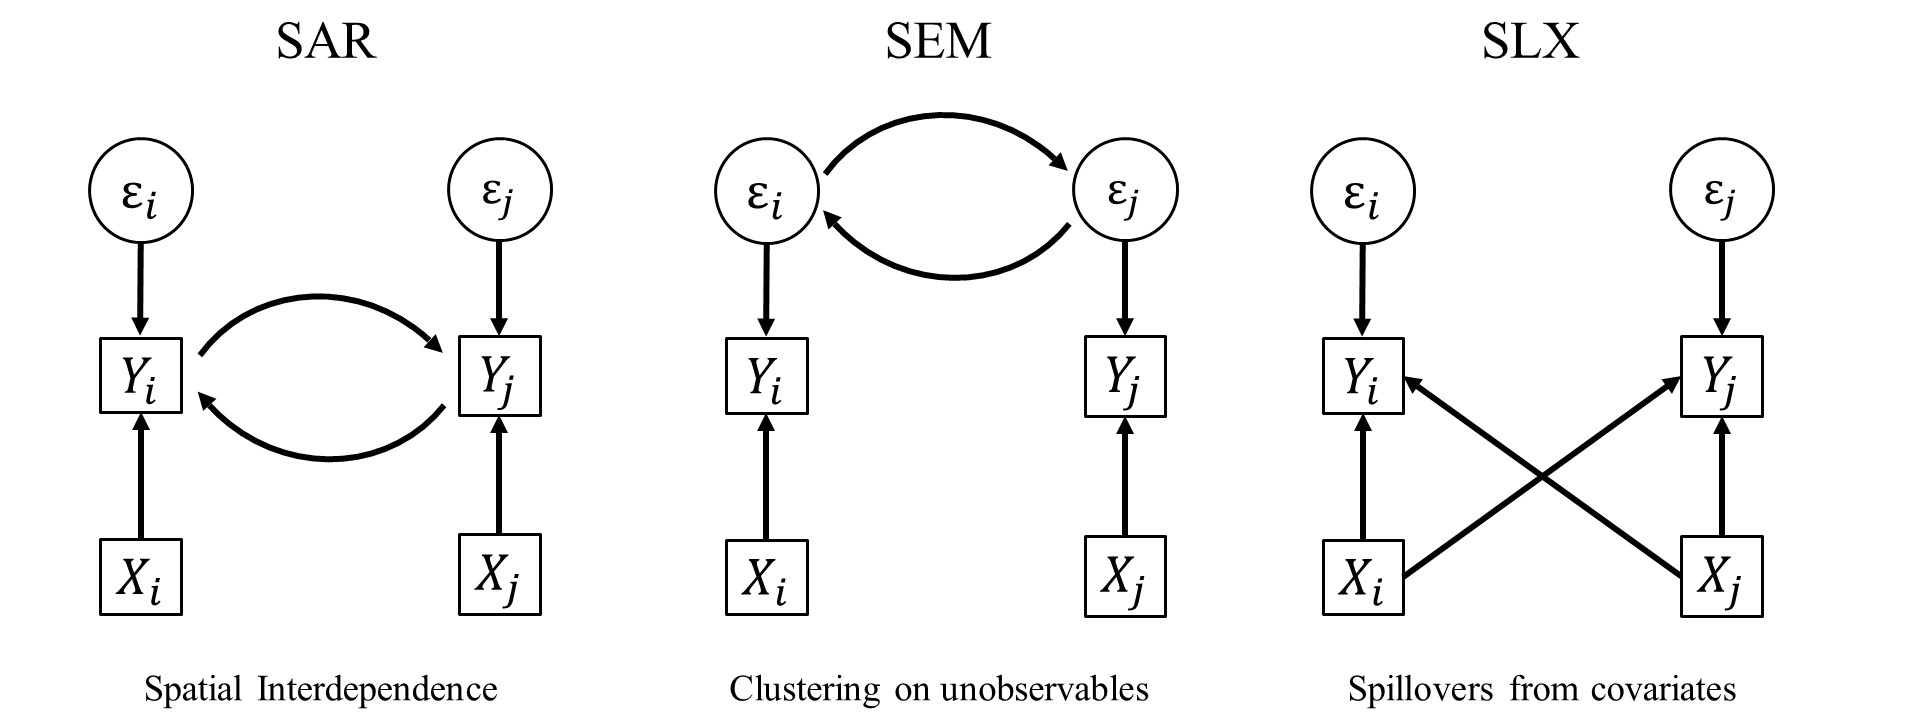
\includegraphics{fig/Graph.jpg}

Note the circular process here: My \(X\) influences my \(Y\), which then
influences your \(Y\), which then influences my \(Y\) again. We write
this as

\[
    \begin{equation} 
        {\boldsymbol{\mathbf{y}}}=\alpha{\boldsymbol{\mathbf{\iota}}}+\rho{\boldsymbol{\mathbf{W}}}{\boldsymbol{\mathbf{y}}}+{\boldsymbol{\mathbf{X}}}{\boldsymbol{\mathbf{\beta}}}+ {\boldsymbol{\mathbf{\varepsilon}}}.
        \end{equation}  
\]

If we ignore \({\boldsymbol{\mathbf{X}}}{\boldsymbol{\mathbf{\beta}}}\)
and write the pure auto-regressive term in its reduce form, we get:

\[
\boldsymbol{\mathbf{y}} =\left(\boldsymbol{\mathbf{I}}_n - \rho\boldsymbol{\mathbf{W}}\right)^{-1}\varepsilon,
\]

and the spatial lag term is

\[
\boldsymbol{\mathbf{W}} \boldsymbol{\mathbf{y}} =\boldsymbol{\mathbf{W}}\left(\boldsymbol{\mathbf{I}}_n - \rho\boldsymbol{\mathbf{W}}\right)^{-1}\varepsilon.
\]

The OLS estimator for the spatial lag term then is

\[
\hat{\rho}_{OLS} = \left[\underbrace{\left(\boldsymbol{\mathbf{W}}\boldsymbol{\mathbf{y}} \right)^\top}_{(1\times n)}\underbrace{\left(\boldsymbol{\mathbf{W}}\boldsymbol{\mathbf{y}} \right)}_{(n\times 1)}\right]^{-1}\underbrace{\left(\boldsymbol{\mathbf{W}}\boldsymbol{\mathbf{y}} \right)^\top}_{(1\times n)}\underbrace{\boldsymbol{\mathbf{y}}}_{(n\times 1)}.
\]

It can then be shown that the OLS estimators equals

\[
          \hat{\rho}_{OLS} = \rho + \left[\left(\boldsymbol{\mathbf{W}}\boldsymbol{\mathbf{y}} \right)^\top\left(\boldsymbol{\mathbf{W}}\boldsymbol{\mathbf{y}} \right)\right]^{-1}\left(\boldsymbol{\mathbf{W}}\boldsymbol{\mathbf{y}} \right)^\top\varepsilon \\
                                = \rho + \left(\sum_{i = 1}^n \boldsymbol{\mathbf{y}}_{Li}^2\right)^{-1}\left(\sum_{i = 1}^{n}\boldsymbol{\mathbf{y}}_{Li}\epsilon_i\right),
\]

with \(\boldsymbol{\mathbf{y}}_{Li}\) defined as the \(i\)th element of
the spatial lag operator
\(\boldsymbol{\mathbf{W}}\boldsymbol{\mathbf{y}} = \boldsymbol{\mathbf{y}}_L\).
It can further be shown that the second part of the equation \(\neq 0\),
which demonstrates that OLS gives a biased estimate of \(\rho\)
(Franzese and Hays 2007; Sarrias 2023).

\begin{tcolorbox}[enhanced jigsaw, opacitybacktitle=0.6, left=2mm, leftrule=.75mm, toptitle=1mm, breakable, colback=white, bottomrule=.15mm, colframe=quarto-callout-warning-color-frame, colbacktitle=quarto-callout-warning-color!10!white, coltitle=black, bottomtitle=1mm, titlerule=0mm, title=\textcolor{quarto-callout-warning-color}{\faExclamationTriangle}\hspace{0.5em}{Warning}, opacityback=0, arc=.35mm, rightrule=.15mm, toprule=.15mm]

Do not estimate spatial lags of the dependent variable in OLS. It will
suffer from simultaneity bias.

\end{tcolorbox}

\hypertarget{instrumental-variable}{%
\section{Instrumental variable}\label{instrumental-variable}}

A potential way of estimating spatial lag /SAR models is 2SLS (Kelejian
and Prucha 1998).

We start with our standard model

\[
        {\boldsymbol{\mathbf{y}}}=\alpha{\boldsymbol{\mathbf{\iota}}}+\rho{\boldsymbol{\mathbf{W}}}{\boldsymbol{\mathbf{y}}}+{\boldsymbol{\mathbf{X}}}{\boldsymbol{\mathbf{\beta}}}+ {\boldsymbol{\mathbf{\varepsilon}}}. 
\]

As we have seen above, there is a problem of simultaneity: the
``covariate'' \({\boldsymbol{\mathbf{W}}}{\boldsymbol{\mathbf{y}}}\) is
endogenous. One way of dealing with this endogeneity problem is the
Instrumental Variable approach.

So, the question is what are good instruments
\(\boldsymbol{\mathbf{H}}\) for
\({\boldsymbol{\mathbf{W}}}{\boldsymbol{\mathbf{y}}}\)? As we have
specified the mode, we are sure that \({\boldsymbol{\mathbf{X}}}\)
determines \({\boldsymbol{\mathbf{y}}}\). Thus, it must be true that
\({\boldsymbol{\mathbf{W}}}{\boldsymbol{\mathbf{X}}}\) and
\({\boldsymbol{\mathbf{W}}}^2{\boldsymbol{\mathbf{X}}},\ldots, {\boldsymbol{\mathbf{W}}}^l{\boldsymbol{\mathbf{X}}}\)
determines \({\boldsymbol{\mathbf{W}}}{\boldsymbol{\mathbf{y}}}\).

Note that \({\boldsymbol{\mathbf{W}}}^l\) denotes higher orders of
\({\boldsymbol{\mathbf{W}}}\). So \({\boldsymbol{\mathbf{W}}}^2\) are
the second order neighbours (neighbours of neighbours), and
\({\boldsymbol{\mathbf{W}}}^3\) are the third order neighbours (the
neighbours of my neighbour's neighbours), and so on\ldots{}

We will discuss this in more detail later, but note for now that the
reduced form of the SAR always contains a series of higher order
neighbours.

\[
({\boldsymbol{\mathbf{I}}_N}-\rho {\boldsymbol{\mathbf{W}}})^{-1}\beta_k 
=({\boldsymbol{\mathbf{I}}_N} + \rho{\boldsymbol{\mathbf{W}}} + \rho^2{\boldsymbol{\mathbf{W}}}^2 + \rho^3{\boldsymbol{\mathbf{W}}}^3 + ...)\beta_k 
= ({\boldsymbol{\mathbf{I}}_N} + \sum_{h=1}^\infty \rho^h{\boldsymbol{\mathbf{W}}}^h)\beta_k .
\]

Thus, Kelejian and Prucha (1998) suggested to use a set of lagged
covariates as instruments for
\(\boldsymbol{\mathbf{W}} \boldsymbol{\mathbf{Y}}\):

\[
\boldsymbol{\mathbf{H}} = \boldsymbol{\mathbf{X}}, \boldsymbol{\mathbf{W}}\boldsymbol{\mathbf{X}}, \boldsymbol{\mathbf{W}}^2\boldsymbol{\mathbf{X}}, ... , \boldsymbol{\mathbf{W}}^l\boldsymbol{\mathbf{X}},
\]

where \(l\) is a pre-defined number for the higher order neighbours
included. In practice, \(l\) is usually restricted to \(l=2\).

This has further been developed by, for instance, using a (truncated)
power series as instruments (Kelejian, Prucha, and Yuzefovich 2004):

\[
\boldsymbol{\mathbf{H}} =\left[\boldsymbol{\mathbf{X}}, \boldsymbol{\mathbf{W}}\left(\sum_{l = 1}^{\infty}\rho^{l}\boldsymbol{\mathbf{W}}^l\right)\boldsymbol{\mathbf{X}} \boldsymbol{\mathbf{\beta}}\right].
\]

We can estimate this using the pacakge \texttt{spatialreg} with the
function \texttt{stsls()},

\begin{Shaded}
\begin{Highlighting}[]
\NormalTok{mod\_1.sls }\OtherTok{\textless{}{-}} \FunctionTok{stsls}\NormalTok{(}\FunctionTok{log}\NormalTok{(med\_house\_price) }\SpecialCharTok{\textasciitilde{}} \FunctionTok{log}\NormalTok{(no2) }\SpecialCharTok{+} \FunctionTok{log}\NormalTok{(POPDEN) }\SpecialCharTok{+} 
\NormalTok{                     per\_mixed }\SpecialCharTok{+}\NormalTok{ per\_asian }\SpecialCharTok{+}\NormalTok{ per\_black }\SpecialCharTok{+}\NormalTok{ per\_other,  }
                   \AttributeTok{data =}\NormalTok{ msoa.spdf, }
                   \AttributeTok{listw =}\NormalTok{ queens.lw,}
                   \AttributeTok{robust =} \ConstantTok{TRUE}\NormalTok{, }\CommentTok{\#  heteroskedasticity robust SEs}
                   \AttributeTok{W2X =} \ConstantTok{TRUE}\NormalTok{) }\CommentTok{\# Second order neighbours are included as instruments (else only first)}
\FunctionTok{summary}\NormalTok{(mod\_1.sls)}
\end{Highlighting}
\end{Shaded}

\begin{verbatim}

Call:stsls(formula = log(med_house_price) ~ log(no2) + log(POPDEN) + 
    per_mixed + per_asian + per_black + per_other, data = msoa.spdf, 
    listw = queens.lw, robust = TRUE, W2X = TRUE)

Residuals:
       Min         1Q     Median         3Q        Max 
-0.5464924 -0.1238002 -0.0052299  0.0989150  1.0793093 

Coefficients: 
               Estimate HC0 std. Error z value  Pr(>|z|)
Rho          0.71004211     0.04678235 15.1776 < 2.2e-16
(Intercept)  2.73582523     0.50997823  5.3646 8.113e-08
log(no2)     0.37752751     0.04920257  7.6729 1.688e-14
log(POPDEN) -0.05710992     0.01684036 -3.3913 0.0006957
per_mixed    0.01634307     0.00588488  2.7771 0.0054842
per_asian   -0.00205426     0.00045905 -4.4750 7.640e-06
per_black   -0.01166456     0.00128557 -9.0734 < 2.2e-16
per_other   -0.00280423     0.00332302 -0.8439 0.3987377

Residual variance (sigma squared): 0.035213, (sigma: 0.18765)
\end{verbatim}

\hypertarget{generalized-method-of-moments}{%
\section{Generalized Method of
Moments}\label{generalized-method-of-moments}}

Generalized Method of Moments (GMM) provides a way of estimating spatial
error / SEM models. A motivation for GMM was that Maximum Likelihood was
unfeasible for large samples and its consistent could not be shown.
Kelejian and Prucha (1999) thus proposed a Moments estimator for SEM.

We start with the model

\[
        \begin{equation} 
        \begin{split}
        {\boldsymbol{\mathbf{y}}}&=\alpha{\boldsymbol{\mathbf{\iota}}}+{\boldsymbol{\mathbf{X}}}{\boldsymbol{\mathbf{\beta}}}+{\boldsymbol{\mathbf{u}}},\\
        {\boldsymbol{\mathbf{u}}}&=\lambda{\boldsymbol{\mathbf{W}}}{\boldsymbol{\mathbf{u}}}+{\boldsymbol{\mathbf{\varepsilon}}}
        \end{split} 
        \end{equation}
\]

The key issue here is to find a consistent estimator for \(\lambda\).
However, we usually do not want to draw inference about \(\lambda\)
itself, but only need it to consistently estimate
\(\boldsymbol{\mathbf{\beta}}\). Kelejian and Prucha (1999) thus treat
\(\lambda\) as pure nuisance paramter.

In essence, the GMM works as follows (Sarrias 2023):

\begin{enumerate}
\def\labelenumi{\arabic{enumi})}
\item
  First of all obtain a consistent estimate of
  \(\boldsymbol{\mathbf{\beta}}\), say
  \(\widetilde{\boldsymbol{\mathbf{\beta}}}\) using either OLS or
  non-linear least squares (NLS).
\item
  Use this estimate to obtain an estimate of
  \(\boldsymbol{\mathbf{u}}\), say
  \(\widehat{\boldsymbol{\mathbf{u}}}\),
\item
  Use \(\widehat{\boldsymbol{\mathbf{u}}}\), to estimate \(\lambda\),
  say \(\widehat{\lambda}\), using
\end{enumerate}

\[
  (\widehat{\lambda}_{NLS, n}, \widehat{\sigma}^2_{NLS, N}) = \mathrm{argmin} \left\lbrace \boldsymbol{\mathbf{\upsilon}}_n(\lambda, \sigma^2)^\top\boldsymbol{\mathbf{\upsilon}}_n(\lambda, \sigma^2): \rho \in [-a, a], \sigma^2\in [0, b]\right\rbrace, 
\]

\begin{enumerate}
\def\labelenumi{\arabic{enumi})}
\setcounter{enumi}{3}
\tightlist
\item
  Estimate \(\boldsymbol{\mathbf{\beta}}\) using Equation
\end{enumerate}

\[
\begin{split}
\boldsymbol{\mathbf{\beta}}_{FGLS}(\lambda) &=\left[\boldsymbol{\mathbf{X}}^\top\boldsymbol{\mathbf{\Omega}}(\widehat{\lambda})^{-1}\boldsymbol{\mathbf{X}}\right]^{-1}\boldsymbol{\mathbf{X}}^\top\boldsymbol{\mathbf{\Omega}}(\widehat{\lambda})^{-1}\boldsymbol{\mathbf{y}}.\\
\boldsymbol{\mathbf{\Omega}}(\lambda) &= (\boldsymbol{\mathbf{I}} - \lambda\boldsymbol{\mathbf{W}})^{-1}(\boldsymbol{\mathbf{I}} - \lambda\boldsymbol{\mathbf{W}}^\top)^{-1}
\end{split}
\]

For more, see for instance Kelejian and Piras (2017), chapter 2.2.4 or
Sarrias (2023).

We can calculate the estimator using \texttt{GMerrorsar()} from
\texttt{spatialreg}.

\begin{Shaded}
\begin{Highlighting}[]
\NormalTok{mod\_1.gmm }\OtherTok{\textless{}{-}} \FunctionTok{GMerrorsar}\NormalTok{(}\FunctionTok{log}\NormalTok{(med\_house\_price) }\SpecialCharTok{\textasciitilde{}} \FunctionTok{log}\NormalTok{(no2) }\SpecialCharTok{+} \FunctionTok{log}\NormalTok{(POPDEN) }\SpecialCharTok{+} 
\NormalTok{                     per\_mixed }\SpecialCharTok{+}\NormalTok{ per\_asian }\SpecialCharTok{+}\NormalTok{ per\_black }\SpecialCharTok{+}\NormalTok{ per\_other,  }
                   \AttributeTok{data =}\NormalTok{ msoa.spdf, }
                   \AttributeTok{listw =}\NormalTok{ queens.lw,}
                   \AttributeTok{se.lambda =} \ConstantTok{TRUE}\NormalTok{) }\CommentTok{\# Provide standard error for lambda}
\FunctionTok{summary}\NormalTok{(mod\_1.gmm)}
\end{Highlighting}
\end{Shaded}

\begin{verbatim}

Call:GMerrorsar(formula = log(med_house_price) ~ log(no2) + log(POPDEN) + 
    per_mixed + per_asian + per_black + per_other, data = msoa.spdf, 
    listw = queens.lw, se.lambda = TRUE)

Residuals:
       Min         1Q     Median         3Q        Max 
-0.8275979 -0.1840855 -0.0096616  0.1610019  1.2270026 

Type: GM SAR estimator
Coefficients: (GM standard errors) 
               Estimate  Std. Error  z value  Pr(>|z|)
(Intercept) 11.07612114  0.26596129  41.6456 < 2.2e-16
log(no2)     0.67758095  0.08620995   7.8597 3.775e-15
log(POPDEN) -0.08006377  0.01464953  -5.4653 4.622e-08
per_mixed   -0.01307831  0.00894766  -1.4616    0.1438
per_asian   -0.00521983  0.00090937  -5.7400 9.465e-09
per_black   -0.01957288  0.00134527 -14.5494 < 2.2e-16
per_other   -0.00521695  0.00489760  -1.0652    0.2868

Lambda: 0.69344 (standard error): 0.071248 (z-value): 9.7328
Residual variance (sigma squared): 0.037126, (sigma: 0.19268)
GM argmin sigma squared: 0.037239
Number of observations: 983 
Number of parameters estimated: 9 
\end{verbatim}

\hypertarget{maximum-likelihood-estimation}{%
\section{Maximum likelihood
estimation}\label{maximum-likelihood-estimation}}

\hypertarget{ml-sar}{%
\subsection{ML SAR}\label{ml-sar}}

Maximum Likelihood estimation of spatial models is the most common way
of estimation. The procedure to estimate Sar models via ML is based on
Ord (1975) and Anselin (1988).

Starting with

\[
\begin{split}
    \boldsymbol{\mathbf{y}}  = \rho \boldsymbol{\mathbf{W}}\boldsymbol{\mathbf{y}} + \boldsymbol{\mathbf{X}}\boldsymbol{\mathbf{\beta }}+ \varepsilon, \\
     \varepsilon  \sim \mathcal{N}(\boldsymbol{\mathbf{0}}_n , \sigma^2\boldsymbol{\mathbf{I}}_n),
\end{split}     
\]

and its reduced form

\[
\begin{split}
{\boldsymbol{\mathbf{y}}} =({\boldsymbol{\mathbf{I}}_N}-\rho {\boldsymbol{\mathbf{W}}})^{-1}({\boldsymbol{\mathbf{X}}}{\boldsymbol{\mathbf{\beta}}}+ {\boldsymbol{\mathbf{\varepsilon}}}), \\
{\boldsymbol{\mathbf{y}}} =\boldsymbol{\mathbf{A}}^{-1}({\boldsymbol{\mathbf{X}}}{\boldsymbol{\mathbf{\beta}}}+ {\boldsymbol{\mathbf{\varepsilon}}}),
\end{split}
\]

where
\(\boldsymbol{\mathbf{A}} = ({\boldsymbol{\mathbf{I}}_N}-\rho {\boldsymbol{\mathbf{W}}})\).

The ML estimator then choses the parameters \(\hat\rho\),
\(\hat{\boldsymbol{\mathbf{\beta}}}\), and \(\hat\sigma\) to maximize
the probability of fitting the observed sample based on the Likelihood
function

\[
\begin{split}
\mathcal{L} (\boldsymbol{\mathbf{\theta}}) &= \log\left| \boldsymbol{\mathbf{A}}\right| - \frac{n\log(2\pi)}{2} - \frac{n\log(\sigma^2)}{2} - \frac{1}{2\sigma^2}(\boldsymbol{\mathbf{A}}\boldsymbol{\mathbf{y}}-\boldsymbol{\mathbf{X}}\boldsymbol{\mathbf{\beta}})^\top (\boldsymbol{\mathbf{A}}\boldsymbol{\mathbf{y}}-\boldsymbol{\mathbf{X}}\boldsymbol{\mathbf{\beta}}) \\
&= \log\left| \boldsymbol{\mathbf{A}}\right| - \frac{n\log(2\pi)}{2} - \frac{n\log(\sigma^2)}{2} - \frac{1}{2\sigma^2}\left[\boldsymbol{\mathbf{y}}^\top \boldsymbol{\mathbf{A}}^\top\boldsymbol{\mathbf{A}}\boldsymbol{\mathbf{y}} - 2\left(\boldsymbol{\mathbf{A}}\boldsymbol{\mathbf{y}}\right)^\top\boldsymbol{\mathbf{X}}\boldsymbol{\mathbf{\beta }}+ \boldsymbol{\mathbf{\beta}}^\top\boldsymbol{\mathbf{X}}^\top\boldsymbol{\mathbf{X}}\boldsymbol{\mathbf{\beta}}\right],
\end{split}
\]

ML estimation of the SAR works as follows Sarrias (2023):

\begin{enumerate}
\def\labelenumi{\arabic{enumi})}
\item
  Perform the two auxiliary regression of \(\boldsymbol{\mathbf{y}}\)
  and \(\boldsymbol{\mathbf{W}}\boldsymbol{\mathbf{y}}\) on
  \(\boldsymbol{\mathbf{X}}\) to obtain the estimators
  \(\widehat{\boldsymbol{\mathbf{\beta}}}_O\) and
  \(\widehat{\boldsymbol{\mathbf{\beta}}}_L\) as in Equation \[
  \begin{split}
  \widehat{\boldsymbol{\mathbf{\beta}}}_{ML}(\rho) &= \left(\boldsymbol{\mathbf{X}}^\top\boldsymbol{\mathbf{X}}\right)^{-1}\boldsymbol{\mathbf{X}}^\top\boldsymbol{\mathbf{y}} - \rho\left(\boldsymbol{\mathbf{X}}^\top\boldsymbol{\mathbf{X}}\right)^{-1}\boldsymbol{\mathbf{X}}^\top\boldsymbol{\mathbf{W}}\boldsymbol{\mathbf{y}}, \\
  &= \widehat{\boldsymbol{\mathbf{\beta}}}_O -\rho \widehat{\boldsymbol{\mathbf{\beta}}}_L.
  \end{split}
  \]
\item
  Use \(\widehat{\boldsymbol{\mathbf{\beta}}}_O\) and
  \(\widehat{\boldsymbol{\mathbf{\beta}}}_L\) to compute the residuals
  in Equation \[
  \varepsilon_O = \boldsymbol{\mathbf{y}} - \boldsymbol{\mathbf{X}}\widehat{\boldsymbol{\mathbf{\beta}}}_0\,\,\mbox{and} \;\; \varepsilon_L = \boldsymbol{\mathbf{W}}\boldsymbol{\mathbf{y}} - \boldsymbol{\mathbf{X}}\widehat{\boldsymbol{\mathbf{\beta}}_L}.
  \]
\item
  By numerical optimization to obtain an estimate of \(\rho\), maximize
  the concentrated likelihood given in
\end{enumerate}

\[
\ell(\rho)=-\frac{n}{2}-\frac{n}{2}\log(2\pi) - \frac{n}{2}\log\left[\frac{\left(\varepsilon_O - \rho\varepsilon_L\right)^\top\left(\varepsilon_O - \rho\varepsilon_L\right)}{n}\right] + \log\left|\boldsymbol{\mathbf{I}}_n - \rho\boldsymbol{\mathbf{W}}\right|,
\]

\begin{enumerate}
\def\labelenumi{\arabic{enumi})}
\setcounter{enumi}{3}
\tightlist
\item
  Use the estimate of \(\widehat{\rho}\) to plug it back in to the
  expression for \(\boldsymbol{\mathbf{\beta}}\) and \(\sigma^2\)
\end{enumerate}

\[
\begin{split}
\widehat{\boldsymbol{\mathbf{\beta}}}_{ML}(\rho) = \left(\boldsymbol{\mathbf{X}}^\top\boldsymbol{\mathbf{X}}\right)^{-1}\boldsymbol{\mathbf{X}}^\top\boldsymbol{\mathbf{A}}\boldsymbol{\mathbf{y}}
\widehat{\sigma}^2_{ML}(\rho) =\\ 
\frac{\left(\boldsymbol{\mathbf{A}}\boldsymbol{\mathbf{y}} - \boldsymbol{\mathbf{X}}\boldsymbol{\mathbf{\beta}}_{ML}\right)^\top\left(\boldsymbol{\mathbf{A}}\boldsymbol{\mathbf{y}} - \boldsymbol{\mathbf{X}}\boldsymbol{\mathbf{\beta}}_{ML}\right)}{n}
\end{split}
\]

\hypertarget{ml-sem}{%
\subsection{ML SEM}\label{ml-sem}}

We can also use ML to estimate the spatial error / SEM model of the form

\[
        \begin{equation} 
        \begin{split}
        {\boldsymbol{\mathbf{y}}}&=\alpha{\boldsymbol{\mathbf{\iota}}}+{\boldsymbol{\mathbf{X}}}{\boldsymbol{\mathbf{\beta}}}+{\boldsymbol{\mathbf{u}}},\\
        {\boldsymbol{\mathbf{u}}}&=\lambda{\boldsymbol{\mathbf{W}}}{\boldsymbol{\mathbf{u}}}+{\boldsymbol{\mathbf{\varepsilon}}}\\
        \varepsilon  &\sim \mathcal{N}(\boldsymbol{\mathbf{0}}_n , \sigma^2\boldsymbol{\mathbf{I}}_n)
        \end{split} 
        \end{equation}
\] Its reduce for is given by

\[
        \begin{equation} 
        \begin{split}
        {\boldsymbol{\mathbf{y}}}&=\alpha{\boldsymbol{\mathbf{\iota}}}+{\boldsymbol{\mathbf{X}}}{\boldsymbol{\mathbf{\beta}}}+({\boldsymbol{\mathbf{I}}_N}-\lambda {\boldsymbol{\mathbf{W}}})^{-1}{\boldsymbol{\mathbf{\varepsilon}}}.\\
        {\boldsymbol{\mathbf{y}}}&=\alpha{\boldsymbol{\mathbf{\iota}}}+{\boldsymbol{\mathbf{X}}}{\boldsymbol{\mathbf{\beta}}}+\boldsymbol{\mathbf{B}}^{-1}{\boldsymbol{\mathbf{\varepsilon}}}.
        \end{split} 
        \end{equation}
\]

where
\(\boldsymbol{\mathbf{B}} = ({\boldsymbol{\mathbf{I}}_N}-\lambda {\boldsymbol{\mathbf{W}}})\).

Note that the OLS estimate of the SEM model are unbiased -- if there is
no omitted variable bias! However, even in that case, they are
inefficient if \(\lambda \neq 0\).

The log-likelihood function is given by

\[
\begin{split}
\ell(\boldsymbol{\mathbf{\theta}}) = - \frac{n}{2}\log(2\pi) - \frac{n}{2}\log(\sigma^2)-\frac{(\boldsymbol{\mathbf{y}} - \boldsymbol{\mathbf{X}}\boldsymbol{\mathbf{\beta}})^\top \boldsymbol{\mathbf{\Omega}}(\lambda) (\boldsymbol{\mathbf{y}} - \boldsymbol{\mathbf{X}}\boldsymbol{\mathbf{\beta}})}{2\sigma^2} + \log\left|\boldsymbol{\mathbf{I}}_n - \lambda \boldsymbol{\mathbf{W}}\right|, \\
\boldsymbol{\mathbf{\Omega}}(\lambda) = \boldsymbol{\mathbf{B}}^\top \boldsymbol{\mathbf{B}} = \left(\boldsymbol{\mathbf{I}}_n-\lambda\boldsymbol{\mathbf{W}}\right)^\top \left(\boldsymbol{\mathbf{I}}_n-\lambda\boldsymbol{\mathbf{W}}\right)
\end{split}
\]

Based on Anselin and Bera (1998), the ML estimation of SEM follow the
procedure (Sarrias 2023):

\begin{enumerate}
\def\labelenumi{\arabic{enumi})}
\item
  Carry out an OLS of \(\boldsymbol{\mathbf{B}}\boldsymbol{\mathbf{X}}\)
  on \(\boldsymbol{\mathbf{B}}\boldsymbol{\mathbf{y}}\); get
  \(\widehat{\boldsymbol{\mathbf{\beta}}}_{OLS}\)
\item
  Compute initial set of residuals
  \(\widehat{\epsilon}_{OLS} = \boldsymbol{\mathbf{B}}\boldsymbol{\mathbf{y}} - \boldsymbol{\mathbf{B}}\boldsymbol{\mathbf{X}}\widehat{\boldsymbol{\mathbf{\beta}}}_{OLS}\)
\item
  Given \$\widehat{\epsilon}\_\{OLS\} \$, find \(\widehat{\lambda}\)
  that maximizes the concentrated likelihood
\end{enumerate}

\[
\ell(\lambda)= \mbox{const} + \frac{n}{2}\log\left[\frac{1}{n}\widehat{\boldsymbol{\mathbf{\varepsilon}}}^\top\boldsymbol{\mathbf{B}}^\top\boldsymbol{\mathbf{B}} \widehat{\boldsymbol{\mathbf{\varepsilon}}}\right] + \log\left|\boldsymbol{\mathbf{B}}\right|.
\]

\begin{enumerate}
\def\labelenumi{\arabic{enumi})}
\setcounter{enumi}{3}
\item
  If the convergence criterion is met, proceed, otherwise repeat steps
  1, 2 and 3.
\item
  Given \(\widehat{\lambda}\), estimate
  \(\widehat{\boldsymbol{\mathbf{\beta}}}(\lambda)\) by GLS and obtain a
  new vector of residuals,
  \(\widehat{\boldsymbol{\mathbf{\varepsilon}}}(\lambda)\)
\item
  Given \(\widehat{\boldsymbol{\mathbf{\varepsilon}}}(\lambda)\) and
  \(\widehat{\lambda}\), estimate \(\widehat{\sigma}(\lambda)\).
\end{enumerate}

The package \texttt{spatialreg} Pebesma and Bivand (2023) provides a
series of functions to calculate the ML estimator for all spatial models
we have considered.

Table from Pebesma and Bivand (2023):

\begin{longtable}[]{@{}
  >{\raggedright\arraybackslash}p{(\columnwidth - 4\tabcolsep) * \real{0.0875}}
  >{\raggedright\arraybackslash}p{(\columnwidth - 4\tabcolsep) * \real{0.4125}}
  >{\raggedright\arraybackslash}p{(\columnwidth - 4\tabcolsep) * \real{0.5000}}@{}}
\toprule\noalign{}
\begin{minipage}[b]{\linewidth}\raggedright
model
\end{minipage} & \begin{minipage}[b]{\linewidth}\raggedright
model name
\end{minipage} & \begin{minipage}[b]{\linewidth}\raggedright
maximum likelihood estimation function
\end{minipage} \\
\midrule\noalign{}
\endhead
\bottomrule\noalign{}
\endlastfoot
SEM & spatial error & \texttt{errorsarlm(...,\ Durbin=FALSE)} \\
SEM & spatial error & \texttt{spautolm(...,\ family="SAR")} \\
SDEM & spatial Durbin error & \texttt{errorsarlm(...,\ Durbin=TRUE)} \\
SLM & spatial lag & \texttt{lagsarlm(...,\ Durbin=FALSE)} \\
SDM & spatial Durbin & \texttt{lagsarlm(...,\ Durbin=TRUE)} \\
SAC & spatial autoregressive combined &
\texttt{sacsarlm(...,\ Durbin=FALSE)} \\
GNM & general nested & \texttt{sacsarlm(...,\ Durbin=TRUE)} \\
\end{longtable}

\textbf{ML SAR}

\begin{Shaded}
\begin{Highlighting}[]
\NormalTok{mod\_1.sar }\OtherTok{\textless{}{-}} \FunctionTok{lagsarlm}\NormalTok{(}\FunctionTok{log}\NormalTok{(med\_house\_price) }\SpecialCharTok{\textasciitilde{}} \FunctionTok{log}\NormalTok{(no2) }\SpecialCharTok{+} \FunctionTok{log}\NormalTok{(POPDEN) }\SpecialCharTok{+} 
\NormalTok{                        per\_mixed }\SpecialCharTok{+}\NormalTok{ per\_asian }\SpecialCharTok{+}\NormalTok{ per\_black }\SpecialCharTok{+}\NormalTok{ per\_other,  }
                      \AttributeTok{data =}\NormalTok{ msoa.spdf, }
                      \AttributeTok{listw =}\NormalTok{ queens.lw,}
                      \AttributeTok{Durbin =} \ConstantTok{FALSE}\NormalTok{) }\CommentTok{\# we could here extend to SDM}
\FunctionTok{summary}\NormalTok{(mod\_1.sar)}
\end{Highlighting}
\end{Shaded}

\begin{verbatim}

Call:lagsarlm(formula = log(med_house_price) ~ log(no2) + log(POPDEN) + 
    per_mixed + per_asian + per_black + per_other, data = msoa.spdf, 
    listw = queens.lw, Durbin = FALSE)

Residuals:
       Min         1Q     Median         3Q        Max 
-0.5281789 -0.1220524 -0.0099245  0.0992203  1.0936745 

Type: lag 
Coefficients: (asymptotic standard errors) 
               Estimate  Std. Error  z value  Pr(>|z|)
(Intercept)  3.17383180  0.29041604  10.9286 < 2.2e-16
log(no2)     0.39705423  0.04452880   8.9168 < 2.2e-16
log(POPDEN) -0.05583014  0.01242876  -4.4920 7.055e-06
per_mixed    0.01851577  0.00579832   3.1933  0.001407
per_asian   -0.00228346  0.00045876  -4.9775 6.442e-07
per_black   -0.01263650  0.00100282 -12.6009 < 2.2e-16
per_other   -0.00161419  0.00289082  -0.5584  0.576582

Rho: 0.66976, LR test value: 473.23, p-value: < 2.22e-16
Asymptotic standard error: 0.025311
    z-value: 26.461, p-value: < 2.22e-16
Wald statistic: 700.19, p-value: < 2.22e-16

Log likelihood: 196.7203 for lag model
ML residual variance (sigma squared): 0.035402, (sigma: 0.18815)
Number of observations: 983 
Number of parameters estimated: 9 
AIC: -375.44, (AIC for lm: 95.786)
LM test for residual autocorrelation
test value: 8.609, p-value: 0.0033451
\end{verbatim}

\textbf{ML SEM}

\begin{Shaded}
\begin{Highlighting}[]
\NormalTok{mod\_1.sem }\OtherTok{\textless{}{-}} \FunctionTok{errorsarlm}\NormalTok{(}\FunctionTok{log}\NormalTok{(med\_house\_price) }\SpecialCharTok{\textasciitilde{}} \FunctionTok{log}\NormalTok{(no2) }\SpecialCharTok{+} \FunctionTok{log}\NormalTok{(POPDEN) }\SpecialCharTok{+}
\NormalTok{                          per\_mixed }\SpecialCharTok{+}\NormalTok{ per\_asian }\SpecialCharTok{+}\NormalTok{ per\_black }\SpecialCharTok{+}\NormalTok{ per\_other,  }
                        \AttributeTok{data =}\NormalTok{ msoa.spdf, }
                        \AttributeTok{listw =}\NormalTok{ queens.lw,}
                        \AttributeTok{Durbin =} \ConstantTok{FALSE}\NormalTok{) }\CommentTok{\# we could here extend to SDEM}
\FunctionTok{summary}\NormalTok{(mod\_1.sem)}
\end{Highlighting}
\end{Shaded}

\begin{verbatim}

Call:errorsarlm(formula = log(med_house_price) ~ log(no2) + log(POPDEN) + 
    per_mixed + per_asian + per_black + per_other, data = msoa.spdf, 
    listw = queens.lw, Durbin = FALSE)

Residuals:
      Min        1Q    Median        3Q       Max 
-0.581785 -0.105218 -0.012758  0.094430  0.913425 

Type: error 
Coefficients: (asymptotic standard errors) 
               Estimate  Std. Error  z value  Pr(>|z|)
(Intercept) 12.92801104  0.35239139  36.6865 < 2.2e-16
log(no2)     0.15735296  0.10880727   1.4462 0.1481317
log(POPDEN) -0.08316270  0.01254315  -6.6301 3.354e-11
per_mixed   -0.03377962  0.00811054  -4.1649 3.115e-05
per_asian   -0.00413115  0.00096849  -4.2656 1.994e-05
per_black   -0.01653816  0.00126741 -13.0488 < 2.2e-16
per_other   -0.01693012  0.00462999  -3.6566 0.0002556

Lambda: 0.88605, LR test value: 623.55, p-value: < 2.22e-16
Asymptotic standard error: 0.015803
    z-value: 56.068, p-value: < 2.22e-16
Wald statistic: 3143.6, p-value: < 2.22e-16

Log likelihood: 271.8839 for error model
ML residual variance (sigma squared): 0.026911, (sigma: 0.16405)
Number of observations: 983 
Number of parameters estimated: 9 
AIC: -525.77, (AIC for lm: 95.786)
\end{verbatim}

\bookmarksetup{startatroot}

\hypertarget{exercises-ii}{%
\chapter{Exercises II}\label{exercises-ii}}

\newcommand{\Exp}{\mathrm{E}}
\newcommand\given[1][]{\:#1\vert\:}
\newcommand{\Cov}{\mathrm{Cov}}
\newcommand{\Var}{\mathrm{Var}}
\newcommand{\rank}{\mathrm{rank}}
\newcommand{\bm}[1]{\boldsymbol{\mathbf{#1}}}

\hypertarget{required-packages-7}{%
\subsection*{Required packages}\label{required-packages-7}}
\addcontentsline{toc}{subsection}{Required packages}

\begin{Shaded}
\begin{Highlighting}[]
\NormalTok{pkgs }\OtherTok{\textless{}{-}} \FunctionTok{c}\NormalTok{(}\StringTok{"sf"}\NormalTok{, }\StringTok{"mapview"}\NormalTok{, }\StringTok{"spdep"}\NormalTok{, }\StringTok{"spatialreg"}\NormalTok{, }\StringTok{"tmap"}\NormalTok{, }\StringTok{"viridisLite"}\NormalTok{) }\CommentTok{\# note: load spdep first, then spatialreg}
\FunctionTok{lapply}\NormalTok{(pkgs, require, }\AttributeTok{character.only =} \ConstantTok{TRUE}\NormalTok{)}
\end{Highlighting}
\end{Shaded}

\hypertarget{session-info-7}{%
\subsection*{Session info}\label{session-info-7}}
\addcontentsline{toc}{subsection}{Session info}

\begin{Shaded}
\begin{Highlighting}[]
\FunctionTok{sessionInfo}\NormalTok{()}
\end{Highlighting}
\end{Shaded}

\begin{verbatim}
R version 4.4.1 (2024-06-14 ucrt)
Platform: x86_64-w64-mingw32/x64
Running under: Windows 11 x64 (build 22631)

Matrix products: default


locale:
[1] LC_COLLATE=English_United Kingdom.utf8 
[2] LC_CTYPE=English_United Kingdom.utf8   
[3] LC_MONETARY=English_United Kingdom.utf8
[4] LC_NUMERIC=C                           
[5] LC_TIME=English_United Kingdom.utf8    

time zone: Europe/Berlin
tzcode source: internal

attached base packages:
[1] stats     graphics  grDevices utils     datasets  methods   base     

other attached packages:
[1] viridisLite_0.4.2 tmap_3.3-4        spatialreg_1.3-4  Matrix_1.7-0     
[5] spdep_1.3-5       spData_2.3.1      mapview_2.11.2    sf_1.0-16        

loaded via a namespace (and not attached):
 [1] xfun_0.45          raster_3.6-26      htmlwidgets_1.6.4  lattice_0.22-6    
 [5] tools_4.4.1        crosstalk_1.2.1    LearnBayes_2.15.1  parallel_4.4.1    
 [9] stats4_4.4.1       sandwich_3.1-0     proxy_0.4-27       KernSmooth_2.23-24
[13] satellite_1.0.5    RColorBrewer_1.1-3 leaflet_2.2.2      lifecycle_1.0.4   
[17] compiler_4.4.1     deldir_2.0-4       munsell_0.5.1      terra_1.7-78      
[21] codetools_0.2-20   leafsync_0.1.0     stars_0.6-5        htmltools_0.5.8.1 
[25] class_7.3-22       MASS_7.3-60.2      classInt_0.4-10    lwgeom_0.2-14     
[29] wk_0.9.1           abind_1.4-5        boot_1.3-30        multcomp_1.4-25   
[33] nlme_3.1-164       digest_0.6.35      mvtnorm_1.2-5      splines_4.4.1     
[37] fastmap_1.2.0      grid_4.4.1         colorspace_2.1-0   cli_3.6.2         
[41] magrittr_2.0.3     base64enc_0.1-3    dichromat_2.0-0.1  XML_3.99-0.16.1   
[45] survival_3.6-4     leafem_0.2.3       TH.data_1.1-2      e1071_1.7-14      
[49] scales_1.3.0       sp_2.1-4           rmarkdown_2.27     zoo_1.8-12        
[53] png_0.1-8          coda_0.19-4.1      evaluate_0.24.0    knitr_1.47        
[57] tmaptools_3.1-1    s2_1.1.6           rlang_1.1.4        Rcpp_1.0.12       
[61] glue_1.7.0         DBI_1.2.3          rstudioapi_0.16.0  jsonlite_1.8.8    
[65] R6_2.5.1           units_0.8-5       
\end{verbatim}

\hypertarget{reload-data-from-pervious-session-6}{%
\subsection*{Reload data from pervious
session}\label{reload-data-from-pervious-session-6}}
\addcontentsline{toc}{subsection}{Reload data from pervious session}

\begin{Shaded}
\begin{Highlighting}[]
\FunctionTok{load}\NormalTok{(}\StringTok{"\_data/msoa2\_spatial.RData"}\NormalTok{)}
\end{Highlighting}
\end{Shaded}

\hypertarget{environmental-inequality}{%
\section{Environmental inequality}\label{environmental-inequality}}

How would you investigate the following descriptive research question:
Are immigrant minorities in London exposed to higher levels of
pollution? Also consider the spatial structure. What's your dependent
and what is your independent variable?

\hypertarget{define-a-neigbours-weights-object-of-your-choice}{%
\subsection*{1) Define a neigbours weights object of your
choice}\label{define-a-neigbours-weights-object-of-your-choice}}
\addcontentsline{toc}{subsection}{1) Define a neigbours weights object
of your choice}

Assume a typical neighbourhood would be 2.5km in diameter

\hypertarget{estimate-the-extent-of-spatial-auto-correlation-in-air-pollution}{%
\subsection*{2) Estimate the extent of spatial auto-correlation in air
pollution}\label{estimate-the-extent-of-spatial-auto-correlation-in-air-pollution}}
\addcontentsline{toc}{subsection}{2) Estimate the extent of spatial
auto-correlation in air pollution}

\hypertarget{estimate-a-spatial-sar-regression-model}{%
\subsection*{3) Estimate a Spatial SAR regression
model}\label{estimate-a-spatial-sar-regression-model}}
\addcontentsline{toc}{subsection}{3) Estimate a Spatial SAR regression
model}

\hypertarget{estimate-a-spatial-sem-regression-model}{%
\subsection*{4) Estimate a Spatial SEM regression
model}\label{estimate-a-spatial-sem-regression-model}}
\addcontentsline{toc}{subsection}{4) Estimate a Spatial SEM regression
model}

\hypertarget{estimate-a-spatial-slx-regression-model}{%
\subsection*{5) Estimate a Spatial SLX regression
model}\label{estimate-a-spatial-slx-regression-model}}
\addcontentsline{toc}{subsection}{5) Estimate a Spatial SLX regression
model}

\hypertarget{estimate-a-spatial-durbin-regression-model}{%
\subsection*{6) Estimate a Spatial Durbin regression
model}\label{estimate-a-spatial-durbin-regression-model}}
\addcontentsline{toc}{subsection}{6) Estimate a Spatial Durbin
regression model}

\hypertarget{estimate-a-spatial-durbin-error-regression-model}{%
\subsection*{7) Estimate a Spatial Durbin Error regression
model}\label{estimate-a-spatial-durbin-error-regression-model}}
\addcontentsline{toc}{subsection}{7) Estimate a Spatial Durbin Error
regression model}

\hypertarget{sneak-preview-on-tomorrow-which-of-the-spatial-model-specifications-about-would-you-choose-prefer-in-a-real-world-example}{%
\subsection{8) Sneak preview on tomorrow: Which of the spatial model
specifications about would you choose / prefer in a real world
example?}\label{sneak-preview-on-tomorrow-which-of-the-spatial-model-specifications-about-would-you-choose-prefer-in-a-real-world-example}}

\hypertarget{please-calculate-the-spatially-lagged-value-of-the-median-house-price.}{%
\subsection{9) Please calculate the spatially lagged value of the median
house
price.}\label{please-calculate-the-spatially-lagged-value-of-the-median-house-price.}}

\hypertarget{can-you-use-the-results-of-the-previous-task-to-run-a-non-linear-slx-model-where-you-predict-if-an-msoa-is-within-the-ulez-zone-based-on-the-house-prices-can-you-make-sense-of-the-result}{%
\subsection{10) Can you use the results of the previous task to run a
non-linear SLX model, where you predict if an MSOA is within the ulez
zone based on the house prices? Can you make sense of the
result?}\label{can-you-use-the-results-of-the-previous-task-to-run-a-non-linear-slx-model-where-you-predict-if-an-msoa-is-within-the-ulez-zone-based-on-the-house-prices-can-you-make-sense-of-the-result}}

\bookmarksetup{startatroot}

\hypertarget{spatial-impacts}{%
\chapter{Spatial Impacts}\label{spatial-impacts}}

\newcommand{\Exp}{\mathrm{E}}
\newcommand\given[1][]{\:#1\vert\:}
\newcommand{\Cov}{\mathrm{Cov}}
\newcommand{\Var}{\mathrm{Var}}
\newcommand{\rank}{\mathrm{rank}}
\newcommand{\bm}[1]{\boldsymbol{\mathbf{#1}}}

\hypertarget{required-packages-8}{%
\subsection*{Required packages}\label{required-packages-8}}
\addcontentsline{toc}{subsection}{Required packages}

\begin{Shaded}
\begin{Highlighting}[]
\NormalTok{pkgs }\OtherTok{\textless{}{-}} \FunctionTok{c}\NormalTok{(}\StringTok{"sf"}\NormalTok{, }\StringTok{"mapview"}\NormalTok{, }\StringTok{"spdep"}\NormalTok{, }\StringTok{"spatialreg"}\NormalTok{, }\StringTok{"tmap"}\NormalTok{, }\StringTok{"viridisLite"}\NormalTok{) }\CommentTok{\# note: load spdep first, then spatialreg}
\FunctionTok{lapply}\NormalTok{(pkgs, require, }\AttributeTok{character.only =} \ConstantTok{TRUE}\NormalTok{)}
\end{Highlighting}
\end{Shaded}

\hypertarget{session-info-8}{%
\subsection*{Session info}\label{session-info-8}}
\addcontentsline{toc}{subsection}{Session info}

\begin{Shaded}
\begin{Highlighting}[]
\FunctionTok{sessionInfo}\NormalTok{()}
\end{Highlighting}
\end{Shaded}

\begin{verbatim}
R version 4.4.1 (2024-06-14 ucrt)
Platform: x86_64-w64-mingw32/x64
Running under: Windows 11 x64 (build 22631)

Matrix products: default


locale:
[1] LC_COLLATE=English_United Kingdom.utf8 
[2] LC_CTYPE=English_United Kingdom.utf8   
[3] LC_MONETARY=English_United Kingdom.utf8
[4] LC_NUMERIC=C                           
[5] LC_TIME=English_United Kingdom.utf8    

time zone: Europe/Berlin
tzcode source: internal

attached base packages:
[1] stats     graphics  grDevices utils     datasets  methods   base     

other attached packages:
[1] viridisLite_0.4.2 tmap_3.3-4        spatialreg_1.3-4  Matrix_1.7-0     
[5] spdep_1.3-5       spData_2.3.1      mapview_2.11.2    sf_1.0-16        

loaded via a namespace (and not attached):
 [1] xfun_0.45          raster_3.6-26      htmlwidgets_1.6.4  lattice_0.22-6    
 [5] tools_4.4.1        crosstalk_1.2.1    LearnBayes_2.15.1  parallel_4.4.1    
 [9] stats4_4.4.1       sandwich_3.1-0     proxy_0.4-27       KernSmooth_2.23-24
[13] satellite_1.0.5    RColorBrewer_1.1-3 leaflet_2.2.2      lifecycle_1.0.4   
[17] compiler_4.4.1     deldir_2.0-4       munsell_0.5.1      terra_1.7-78      
[21] codetools_0.2-20   leafsync_0.1.0     stars_0.6-5        htmltools_0.5.8.1 
[25] class_7.3-22       MASS_7.3-60.2      classInt_0.4-10    lwgeom_0.2-14     
[29] wk_0.9.1           abind_1.4-5        boot_1.3-30        multcomp_1.4-25   
[33] nlme_3.1-164       digest_0.6.35      mvtnorm_1.2-5      splines_4.4.1     
[37] fastmap_1.2.0      grid_4.4.1         colorspace_2.1-0   cli_3.6.2         
[41] magrittr_2.0.3     base64enc_0.1-3    dichromat_2.0-0.1  XML_3.99-0.16.1   
[45] survival_3.6-4     leafem_0.2.3       TH.data_1.1-2      e1071_1.7-14      
[49] scales_1.3.0       sp_2.1-4           rmarkdown_2.27     zoo_1.8-12        
[53] png_0.1-8          coda_0.19-4.1      evaluate_0.24.0    knitr_1.47        
[57] tmaptools_3.1-1    s2_1.1.6           rlang_1.1.4        Rcpp_1.0.12       
[61] glue_1.7.0         DBI_1.2.3          rstudioapi_0.16.0  jsonlite_1.8.8    
[65] R6_2.5.1           units_0.8-5       
\end{verbatim}

\hypertarget{reload-data-from-pervious-session-7}{%
\subsection*{Reload data from pervious
session}\label{reload-data-from-pervious-session-7}}
\addcontentsline{toc}{subsection}{Reload data from pervious session}

\begin{Shaded}
\begin{Highlighting}[]
\FunctionTok{load}\NormalTok{(}\StringTok{"\_data/msoa2\_spatial.RData"}\NormalTok{)}
\end{Highlighting}
\end{Shaded}

\hypertarget{coefficient-estimates-neq-marginal-effects}{%
\section{\texorpdfstring{Coefficient estimates \(\neq\) `marginal'
effects}{Coefficient estimates \textbackslash neq `marginal' effects}}\label{coefficient-estimates-neq-marginal-effects}}

\begin{tcolorbox}[enhanced jigsaw, opacitybacktitle=0.6, left=2mm, leftrule=.75mm, toptitle=1mm, breakable, colback=white, bottomrule=.15mm, colframe=quarto-callout-warning-color-frame, colbacktitle=quarto-callout-warning-color!10!white, coltitle=black, bottomtitle=1mm, titlerule=0mm, title=\textcolor{quarto-callout-warning-color}{\faExclamationTriangle}\hspace{0.5em}{Warning}, opacityback=0, arc=.35mm, rightrule=.15mm, toprule=.15mm]

Do not interpret coefficients as marginal effects in SAR, SAC, and SDM!!

\end{tcolorbox}

At first glance, the specifications presented above seem relatively
similar in the way of modelling spatial effects. \textbf{Yet, they
differ in very important aspects}.

First, models with an endogenous spatial term (SAR, SAC, and SDM) assume
a very different spatial dependence structure than models with only
exogenous spatial terms as SLX and SDEM specifications. While the first
three assume \textbf{global} spatial dependence, the second two assume
\textbf{local} spatial dependence (Anselin 2003; Halleck Vega and
Elhorst 2015; LeSage and Pace 2009).

Second, the interpretation of the coefficients differs greatly between
models with and without endogenous effects. This becomes apparent when
considering the reduced form of the equations above. Exemplary using the
SAR model, the reduced form is given by:

\[
\begin{split}
{\boldsymbol{\mathbf{y}}}-\rho{\boldsymbol{\mathbf{W}}}{\boldsymbol{\mathbf{y}}} &={\boldsymbol{\mathbf{X}}}{\boldsymbol{\mathbf{\beta}}}+ {\boldsymbol{\mathbf{\varepsilon}}}, \nonumber \\
({\boldsymbol{\mathbf{I}}_N}-\rho {\boldsymbol{\mathbf{W}}}){\boldsymbol{\mathbf{y}}} &={\boldsymbol{\mathbf{X}}}{\boldsymbol{\mathbf{\beta}}}+ {\boldsymbol{\mathbf{\varepsilon}}}\nonumber, \\
{\boldsymbol{\mathbf{y}}} &=({\boldsymbol{\mathbf{I}}_N}-\rho {\boldsymbol{\mathbf{W}}})^{-1}({\boldsymbol{\mathbf{X}}}{\boldsymbol{\mathbf{\beta}}}+ {\boldsymbol{\mathbf{\varepsilon}}}),
\end{split}
\]

where \({\boldsymbol{\mathbf{I}}_N}\) is an \(N \times N\) diagonal
matrix (diagonal elements equal 1, 0 otherwise). This contains no
spatially lagged dependent variable on the right-hand side.

If we want to interpret coefficient, we are usually in marginal or
partial effects (the association between a unit change in \(X\) and
\(Y\)). We obtain these effects by looking at the first derivative.

When taking the first derivative of the explanatory variable
\({\boldsymbol{\mathbf{x}}}_k\) from the reduced form in
(\ref{eq:sarred}) to interpret the partial effect of a unit change in
variable \({\boldsymbol{\mathbf{x}}}_k\) on
\({\boldsymbol{\mathbf{y}}}\), we receive

\[
\frac{\partial {\boldsymbol{\mathbf{y}}}}{\partial {\boldsymbol{\mathbf{x}}}_k}=\underbrace{({\boldsymbol{\mathbf{I}}_N}-\rho {\boldsymbol{\mathbf{W}}})^{-1}}_{N \times N}\beta_k,
\]

for each covariate \(k=\{1,2,...,K\}\). As can be seen, the partial
derivative with respect to \({\boldsymbol{\mathbf{x}}}_k\) produces an
\(N \times N\) matrix, thereby representing the partial effect of each
unit \(i\) onto the focal unit \(i\) itself and all other units
\textcolor{red}{$j=\{1,2,...,i-1,i+1,...,N\}$}.

Note that the diagonal elements of
\(({\boldsymbol{\mathbf{I}}_N}-\rho {\boldsymbol{\mathbf{W}}})^{-1}\)
are not zero anymore (as they are in \(\boldsymbol{\mathbf{W}}\)). Look
at the following minimal example:

\[
\begin{split}
\tilde{\boldsymbol{\mathbf{W}}} = \begin{pmatrix}
      0 & 1 & 0 & 1 & 0 \\
      1 & 0 & 1 & 0 & 1 \\
      0 & 1 & 0 & 1 & 0 \\
      1 & 0 & 1 & 0 & 1 \\
      0 & 1 & 0 & 1 & 0
      \end{pmatrix}, \mathrm{and~normalized} ~
\boldsymbol{\mathbf{W}} = \begin{pmatrix}
      0 & 0.5 & 0 & 0.5 & 0 \\
      0.33 & 0 & 0.33 & 0 & 0.33 \\
      0 & 0.5 & 0 & 0.5 & 0 \\
      0.33 & 0 & 0.33 & 0 & 0.33 \\
      0 & 0.5 & 0 & 0.5 & 0
      \end{pmatrix}      
\end{split}
\]

and

\[
\rho = 0.6,
\]

then

\[
\begin{split}
\rho \boldsymbol{\mathbf{W}} = \begin{pmatrix}
      0 & 0.3 & 0 & 0.3 & 0 \\
      0.2 & 0 & 0.2 & 0 & 0.2 \\
      0 & 0.3 & 0 & 0.3 & 0 \\
      0.2 & 0 & 0.2 & 0 & 0.2 \\
      0 & 0.3 & 0 & 0.3 & 0
      \end{pmatrix}.
\end{split}
\]

If we want to get the total effect of \(X\) on \(Y\) we need to add the
direct association within \(i\) and \(j\) and so on\ldots{}

\[
\begin{split}
\boldsymbol{\mathbf{I}}_N - \rho \boldsymbol{\mathbf{W}} &=
\begin{pmatrix}
      1 & 0 & 0 & 0 & 0 \\
      0 & 1 & 0 & 0 & 0 \\
      0 & 0 & 1 & 0 & 0 \\
      0 & 0 & 0 & 1 & 0 \\
      0 & 1 & 0 & 0 & 1
      \end{pmatrix} - 
\begin{pmatrix}
      0 & 0.3 & 0 & 0.3 & 0 \\
      0.2 & 0 & 0.2 & 0 & 0.2 \\
      0 & 0.3 & 0 & 0.3 & 0 \\
      0.2 & 0 & 0.2 & 0 & 0.2 \\
      0 & 0.3 & 0 & 0.3 & 0
      \end{pmatrix}\\
& = \begin{pmatrix}
      1 & -0.3 & 0 & -0.3 & 0 \\
      -0.2 & 1 & -0.2 & 0 & -0.2 \\
      0 & 0.3 & 1 & 0.3 & 0 \\
      -0.2 & 0 & -0.2 & 1 & -0.2 \\
      0 & -0.3 & 0 & -0.3 & 1
      \end{pmatrix}.
\end{split}
\]

And finally we take the inverse of that

\[
\begin{split}
(\boldsymbol{\mathbf{I}}_N - \rho \boldsymbol{\mathbf{W}})^{-1} &=
\begin{pmatrix}
      1 & -0.3 & 0 & -0.3 & 0 \\
      -0.2 & 1 & -0.2 & 0 & -0.2 \\
      0 & 0.3 & 1 & 0.3 & 0 \\
      -0.2 & 0 & -0.2 & 1 & -0.2 \\
      0 & -0.3 & 0 & -0.3 & 1
      \end{pmatrix}^{-1}\\
&=
\begin{pmatrix}
      \color{red}{1.1875} & 0.46875 & 0.1875 & 0.46875 & 0.1875 \\
      0.3125 & \color{red}{1.28125} & 0.3125 & 0.28125 & 0.3125 \\
      0.1875 & 0.46875 & \color{red}{1.1875} & 0.46875 & 0.1875 \\
      0.3125 & 0.28125 & 0.3125 & \color{red}{1.28125} & 0.3125 \\
      0.1875 & 0.46875 & 0.1875 & 0.46875 & \color{red}{1.1875}
      \end{pmatrix}.
\end{split}
\]

As you can see,
\((\boldsymbol{\mathbf{I}}_N - \rho \boldsymbol{\mathbf{W}})^{-1}\) has
\color{red}{diagonal elements} \(>1\): these are feedback loops. My
\(X\) influences my \(Y\) directly, but my \(Y\) then influences my
neigbour's \(Y\), which then influences my \(Y\) again (also also other
neighbour's \(Y\)s). Thus the influence of my \(X\) on my \(Y\) includes
a spatial multiplier.

Check yourself:

\begin{Shaded}
\begin{Highlighting}[]
\NormalTok{I }\OtherTok{=} \FunctionTok{diag}\NormalTok{(}\DecValTok{5}\NormalTok{)}
\NormalTok{rho }\OtherTok{=} \FloatTok{0.6}
\NormalTok{W }\OtherTok{=} \FunctionTok{matrix}\NormalTok{(}\FunctionTok{c}\NormalTok{(}\DecValTok{0}\NormalTok{ , }\FloatTok{0.5}\NormalTok{ , }\DecValTok{0}\NormalTok{ , }\FloatTok{0.5}\NormalTok{ , }\DecValTok{0}\NormalTok{,}
            \DecValTok{1}\SpecialCharTok{/}\DecValTok{3}\NormalTok{ , }\DecValTok{0}\NormalTok{ , }\DecValTok{1}\SpecialCharTok{/}\DecValTok{3}\NormalTok{ , }\DecValTok{0}\NormalTok{ , }\DecValTok{1}\SpecialCharTok{/}\DecValTok{3}\NormalTok{,}
            \DecValTok{0}\NormalTok{ , }\FloatTok{0.5}\NormalTok{ , }\DecValTok{0}\NormalTok{ , }\FloatTok{0.5}\NormalTok{ , }\DecValTok{0}\NormalTok{,}
            \DecValTok{1}\SpecialCharTok{/}\DecValTok{3}\NormalTok{ , }\DecValTok{0}\NormalTok{ , }\DecValTok{1}\SpecialCharTok{/}\DecValTok{3}\NormalTok{ , }\DecValTok{0}\NormalTok{ , }\DecValTok{1}\SpecialCharTok{/}\DecValTok{3}\NormalTok{,}
            \DecValTok{0}\NormalTok{ , }\FloatTok{0.5}\NormalTok{ , }\DecValTok{0}\NormalTok{ , }\FloatTok{0.5}\NormalTok{ , }\DecValTok{0}\NormalTok{), }\AttributeTok{ncol =} \DecValTok{5}\NormalTok{, }\AttributeTok{byrow =} \ConstantTok{TRUE}\NormalTok{)}

\NormalTok{(}\AttributeTok{IrW =}\NormalTok{ I }\SpecialCharTok{{-}}\NormalTok{ rho}\SpecialCharTok{*}\NormalTok{W)}
\end{Highlighting}
\end{Shaded}

\begin{verbatim}
     [,1] [,2] [,3] [,4] [,5]
[1,]  1.0 -0.3  0.0 -0.3  0.0
[2,] -0.2  1.0 -0.2  0.0 -0.2
[3,]  0.0 -0.3  1.0 -0.3  0.0
[4,] -0.2  0.0 -0.2  1.0 -0.2
[5,]  0.0 -0.3  0.0 -0.3  1.0
\end{verbatim}

\begin{Shaded}
\begin{Highlighting}[]
\CommentTok{\# (I {-} rho*W)\^{}{-}1}
\NormalTok{(}\AttributeTok{M =} \FunctionTok{solve}\NormalTok{(IrW))}
\end{Highlighting}
\end{Shaded}

\begin{verbatim}
       [,1]    [,2]   [,3]    [,4]   [,5]
[1,] 1.1875 0.46875 0.1875 0.46875 0.1875
[2,] 0.3125 1.28125 0.3125 0.28125 0.3125
[3,] 0.1875 0.46875 1.1875 0.46875 0.1875
[4,] 0.3125 0.28125 0.3125 1.28125 0.3125
[5,] 0.1875 0.46875 0.1875 0.46875 1.1875
\end{verbatim}

The diagonal elements of \(M\) indicate how each unit \(i\) influences
itself (change of \(x_i\) on change of \(y_i\)), and each off-diagonal
elements in column \(j\) represents the effect of \(j\) on each other
unit \(i\) (change of \(x_j\) on change of \(y_i\)).

\[
\begin{split}
\begin{pmatrix}
      1.1875 & \color{red}{0.46875} & 0.1875 & 0.46875 & 0.1875 \\
      0.3125 & 1.28125 & 0.3125 & 0.28125 & 0.3125 \\
      0.1875 & 0.46875 & 1.1875 & 0.46875 & 0.1875 \\
      0.3125 & 0.28125 & 0.3125 & 1.28125 & 0.3125 \\
      0.1875 & 0.46875 & \color{blue}{0.1875} & 0.46875 & 1.1875
      \end{pmatrix}.
\end{split}
\]

For instance, \(\color{red}{W_{12}}\) indicates that unit 2 has an
influence of 0.46875 on unit 1. On the other hand,
\(\color{blue}{W_{53}}\) indicates that unit 3 has an influence of
magnitude 0.1875 on unit 5.

\begin{tcolorbox}[enhanced jigsaw, opacitybacktitle=0.6, left=2mm, leftrule=.75mm, toptitle=1mm, breakable, colback=white, bottomrule=.15mm, colframe=quarto-callout-tip-color-frame, colbacktitle=quarto-callout-tip-color!10!white, coltitle=black, bottomtitle=1mm, titlerule=0mm, title=\textcolor{quarto-callout-tip-color}{\faLightbulb}\hspace{0.5em}{Question}, opacityback=0, arc=.35mm, rightrule=.15mm, toprule=.15mm]

Why does unit 3 have any effect o unit 5? According to
\(\boldsymbol{\mathbf{W}}\) those two units are no neighbours
\(w_{53} = 0\)!

\end{tcolorbox}

\hypertarget{global-and-local-spillovers}{%
\section{Global and local
spillovers}\label{global-and-local-spillovers}}

The kind of indirect spillover effects in SAR, SAC, and SDM models
differs from the kind of indirect spillover effects in SLX and SDEM
models: while the first three specifications represent \textbf{global
spillover effects}, the latter three represent \textbf{local spillover
effects} (Anselin 2003; LeSage and Pace 2009; LeSage 2014a).

\hypertarget{local-spillovers}{%
\subsection{Local spillovers}\label{local-spillovers}}

In case of SLX and SDEM the spatial spillover effects can be interpreted
as the effect of a one unit change of \({\boldsymbol{\mathbf{x}}}_k\) in
the spatially weighted neighbouring observations on the dependent
variable of the focal unit: the weighted average among neighbours; when
using a row-normalised contiguity weights matrix,
\({\boldsymbol{\mathbf{W}}} {\boldsymbol{\mathbf{x}}}_k\) is the mean
value of \({\boldsymbol{\mathbf{x}}}_k\) in the neighbouring units.

Assume we have \(k =2\) covariates, then

\[
\begin{split}
\underbrace{\boldsymbol{\mathbf{W}}}_{N \times N}  \underbrace{\boldsymbol{\mathbf{X}}}_{N \times 2} \underbrace{\boldsymbol{\mathbf{\theta}}}_{2 \times 1} & = 
\begin{pmatrix}
      0 & 0.5 & 0 & 0.5 & 0 \\
      0.33 & 0 & 0.33 & 0 & 0.33 \\
      0 & 0.5 & 0 & 0.5 & 0 \\
      0.33 & 0 & 0.33 & 0 & 0.33 \\
      0 & 0.5 & 0 & 0.5 & 0
  \end{pmatrix}
  \begin{pmatrix}
      3 & 100 \\
      4 & 140 \\
      1 & 200 \\
      7 & 70  \\
      5 & 250 
  \end{pmatrix}
    \begin{pmatrix}
      \theta_1 \\
      \theta_2 
  \end{pmatrix}\\
 & =   
 \begin{pmatrix}
      6 & 105 \\
      3 & 190 \\
      6 & 105 \\
      3 & 190  \\
      6 & 105 
  \end{pmatrix}
 \begin{pmatrix}
      \theta_1 \\
      \theta_2
  \end{pmatrix}\\
\end{split} 
\]

\begin{Shaded}
\begin{Highlighting}[]
\NormalTok{X }\OtherTok{\textless{}{-}} \FunctionTok{cbind}\NormalTok{(}\AttributeTok{x1 =} \FunctionTok{c}\NormalTok{(}\DecValTok{3}\NormalTok{,}\DecValTok{4}\NormalTok{,}\DecValTok{1}\NormalTok{,}\DecValTok{8}\NormalTok{,}\DecValTok{5}\NormalTok{),}
           \AttributeTok{x2 =} \FunctionTok{c}\NormalTok{(}\DecValTok{100}\NormalTok{,}\DecValTok{140}\NormalTok{,}\DecValTok{200}\NormalTok{,}\DecValTok{70}\NormalTok{,}\DecValTok{270}\NormalTok{))}
\NormalTok{(WX }\OtherTok{\textless{}{-}}\NormalTok{  W }\SpecialCharTok{\%*\%}\NormalTok{ X)}
\end{Highlighting}
\end{Shaded}

\begin{verbatim}
     x1  x2
[1,]  6 105
[2,]  3 190
[3,]  6 105
[4,]  3 190
[5,]  6 105
\end{verbatim}

Thus, only direct neighbours -- as defined in
\({\boldsymbol{\mathbf{W}}}\) -- contribute to those local spillover
effects. The \(\hat{\boldsymbol{\mathbf{\theta}}}\) coefficients only
estimate how my direct neighbour's \(\boldsymbol{\mathbf{X}}\) values
influence my own outcome \(\boldsymbol{\mathbf{y}}\).

There are no higher order neighbours involved (as long as we do not
model them), nor are there any feedback loops due to interdependence.

\hypertarget{global-spillovers}{%
\subsection{Global spillovers}\label{global-spillovers}}

In contrast, spillover effects in SAR, SAC, and SDM models do not only
include direct neighbours but also neighbours of neighbours (second
order neighbours) and further higher-order neighbours. This can be seen
by rewriting the inverse
\(({\boldsymbol{\mathbf{I}}_N}-\rho {\boldsymbol{\mathbf{W}}})^{-1}\) as
power series:A power series of
\(\sum\nolimits_{k=0}^\infty {\boldsymbol{\mathbf{W}}}^k\) converges to
\(({\boldsymbol{\mathbf{I}}}-{\boldsymbol{\mathbf{W}}})^{-1}\) if the
maximum absolute eigenvalue of \({\boldsymbol{\mathbf{W}}} < 1\), which
is ensured by standardizing \({\boldsymbol{\mathbf{W}}}\).\}

\[
\begin{split}
({\boldsymbol{\mathbf{I}}_N}-\rho {\boldsymbol{\mathbf{W}}})^{-1}\beta_k 
=({\boldsymbol{\mathbf{I}}_N} + \rho{\boldsymbol{\mathbf{W}}} + \rho^2{\boldsymbol{\mathbf{W}}}^2 + \rho^3{\boldsymbol{\mathbf{W}}}^3 + ...)\beta_k 
= ({\boldsymbol{\mathbf{I}}_N} + \sum_{h=1}^\infty \rho^h{\boldsymbol{\mathbf{W}}}^h)\beta_k ,
\end{split}
\]

where the identity matrix represents the direct effects and the sum
represents the first and higher order indirect effects and the above
mentioned feedback loops. This implies that a change in one unit \(i\)
does not only affect the direct neighbours but passes through the whole
system towards higher-order neighbours, where the impact declines with
distance within the neighbouring system. Global indirect impacts thus
are `multiplied' by influencing direct neighbours as specified in
\(\boldsymbol{\mathbf{W}}\) and indirect neighbours not connected
according to \(\boldsymbol{\mathbf{W}}\), with additional feedback loops
between those neighbours.

\[
\begin{split}
\underbrace{(\underbrace{\boldsymbol{\mathbf{I}}_N}_{N \times N} - \underbrace{\rho}_{\hat{=} 0.6} \underbrace{\boldsymbol{\mathbf{W}}}_{N \times N})^{-1}}_{N \times N} \beta_k
&=
\begin{pmatrix}
      1.\color{red}{1875} & 0.46875 & 0.1875 & 0.46875 & 0.1875 \\
      0.3125 & 1.\color{red}{28125} & 0.3125 & 0.28125 & 0.3125 \\
      0.1875 & 0.46875 & 1.\color{red}{1875} & 0.46875 & 0.1875 \\
      0.3125 & 0.28125 & 0.3125 & 1.\color{red}{28125} & 0.3125 \\
      0.1875 & 0.46875 & 0.1875 & 0.46875 & 1.\color{red}{1875}
      \end{pmatrix}
  \begin{matrix}
      (\beta_1 + \beta_2)\\
  \end{matrix}\\.
\end{split}
\]

All diagonal elements of
\(\mathrm{diag}({\boldsymbol{\mathbf{W}}})=w_{ii}=0\). However, diagonal
elements of higher order neighbours are not zero
\(\mathrm{diag}({\boldsymbol{\mathbf{W}}}^2)=\mathrm{diag}({\boldsymbol{\mathbf{W}}}{\boldsymbol{\mathbf{W}}})\neq0\).

Intuitively, \(\rho{\boldsymbol{\mathbf{W}}}\) only represents the
effects between direct neighbours (and the focal unit is not a neighbour
of the focal unit itself), whereas \(\rho^2{\boldsymbol{\mathbf{W}}}^2\)
contains the effects of second order neighbours, where the focal unit is
a second order neighbour of the focal unit itself. Thus,
\(({\boldsymbol{\mathbf{I}}_N}-\rho {\boldsymbol{\mathbf{W}}})^{-1}\beta_k\)
includes {feedback effects} from \(\rho^2{\boldsymbol{\mathbf{W}}}^2\)
on (they are part of the direct impacts according to the summary
measures below). This is way the {diagonal above} \(\geq 1\).

In consequence, local and global spillover effects represent two
distinct kinds of spatial spillover effects (LeSage 2014a). The
interpretation of local spillover effects is straightforward: it
represents the effect of all neighbours as defined by
\({\boldsymbol{\mathbf{W}}}\) (the average over all neighbours in case
of a row-normalised weights matrix).

For instance, the environmental quality in the focal unit itself but
also in neighbouring units could influence the attractiveness of a
district and its house prices. In this example it seems reasonable to
assume that we have local spillover effects: only the environmental
quality in directly contiguous units (e.g.~in walking distance) is
relevant for estimating the house prices.

In contrast, interpreting global spillover effects can be a bit more
difficult. Intuitively, the global spillover effects can be seen as a
kind of diffusion process. For example, an exogenous event might
increase the house prices in one district of a city, thus leading to an
adaptation of house prices in neighbouring districts, which then leads
to further adaptations in other units (the neighbours of the
neighbours), thereby globally diffusing the effect of the exogenous
event due to the endogenous term.

Yet, those processes happen over time. In a cross-sectional framework,
the global spillover effects are hard to interpret. Anselin (2003)
proposes an interpretation as an equilibrium outcome, where the partial
impact represents an estimate of how this long-run equilibrium would
change due to a change in \({\boldsymbol{\mathbf{x}}}_k\) (LeSage
2014a).

\hypertarget{summary-impact-measures}{%
\section{Summary impact measures}\label{summary-impact-measures}}

Note that the derivative in SAR, SAC, and SDM is a \(N \times N\)
matrix, returning individual effects of each unit on each other unit,
differentiated in \emph{direct, indirect, and total impacts}.

\[
\begin{split}
(\boldsymbol{\mathbf{I}}_N - \rho \boldsymbol{\mathbf{W}})^{-1} \beta &=
\begin{pmatrix}
      \color{red}{1.1875} & \color{blue}{0.46875} & \color{blue}{0.1875} & \color{blue}{0.46875} & \color{blue}{0.1875} \\
      \color{blue}{0.3125} & \color{red}{1.28125} & \color{blue}{0.3125} & \color{blue}{0.28125} & \color{blue}{0.3125} \\
      \color{blue}{0.1875} & \color{blue}{0.46875} & \color{red}{1.1875} & \color{blue}{0.46875} & \color{blue}{0.1875} \\
      \color{blue}{0.3125} & \color{blue}{0.28125} & \color{blue}{0.3125} & \color{red}{1.28125} & \color{blue}{0.3125} \\
      \color{blue}{0.1875} & \color{blue}{0.46875} & \color{blue}{0.1875} & \color{blue}{0.46875} & \color{red}{1.1875}
      \end{pmatrix} \beta
\end{split}
\]

\textbf{However, the individual effects (how \(i\) influences \(j\))
mainly vary because of variation in \({\boldsymbol{\mathbf{W}}}\). }

\begin{tcolorbox}[enhanced jigsaw, opacitybacktitle=0.6, left=2mm, leftrule=.75mm, toptitle=1mm, breakable, colback=white, bottomrule=.15mm, colframe=quarto-callout-warning-color-frame, colbacktitle=quarto-callout-warning-color!10!white, coltitle=black, bottomtitle=1mm, titlerule=0mm, title=\textcolor{quarto-callout-warning-color}{\faExclamationTriangle}\hspace{0.5em}{Do not interpret these as ``estimated'' individual impacts}, opacityback=0, arc=.35mm, rightrule=.15mm, toprule=.15mm]

We estimate two scalar parameters in a SAR model: \(\beta\) for the
direct coefficient and \(rho\) for the auto-regressive parameter.

All variation in the effects matrix
\((\boldsymbol{\mathbf{I}}_N - \rho \boldsymbol{\mathbf{W}})^{-1}\)
\beta comes from the relationship in \(\boldsymbol{\mathbf{W}}\) which
we have given a-priori!

\end{tcolorbox}

Since reporting the individual partial effects is usually not of
interest, LeSage and Pace (2009) proposed to average over these effect
matrices. While the average diagonal elements of the effects matrix
\((\boldsymbol{\mathbf{I}}_N - \rho \boldsymbol{\mathbf{W}})^{-1}\)
represent the so called direct impacts of variable
\({\boldsymbol{\mathbf{x}}}_k\), the average column-sums of the
off-diagonal elements represent the so called indirect impacts (or
spatial spillover effects).

{direct impacts} refer to an average effect of a unit change in \(x_i\)
on \(y_i\), and {the indirect (spillover) impacts} indicate how a change
in \(x_i\), on average, influences all neighbouring units \(y_j\).

Though previous literature (Halleck Vega and Elhorst 2015; LeSage and
Pace 2009) has established the notation of direct and indirect impacts,
it is important to note that also the direct impacts comprise a spatial
`multiplier' component if we specify an endogenous lagged depended
variable, as a change in \(\boldsymbol{\mathbf{x}}_i\) influences
\(\boldsymbol{\mathbf{y}}_i\), which influences
\(\boldsymbol{\mathbf{y}}_j\), which in turn influences
\(\boldsymbol{\mathbf{y}}_i\).

Usually, one should use summary measures to report effects in spatial
models (LeSage and Pace 2009). Halleck Vega and Elhorst (2015) provide a
nice summary of the impacts for each model:

\begin{longtable}[]{@{}
  >{\centering\arraybackslash}p{(\columnwidth - 6\tabcolsep) * \real{0.2500}}
  >{\centering\arraybackslash}p{(\columnwidth - 6\tabcolsep) * \real{0.2500}}
  >{\centering\arraybackslash}p{(\columnwidth - 6\tabcolsep) * \real{0.2500}}
  >{\centering\arraybackslash}p{(\columnwidth - 6\tabcolsep) * \real{0.2500}}@{}}
\toprule\noalign{}
\begin{minipage}[b]{\linewidth}\centering
Model
\end{minipage} & \begin{minipage}[b]{\linewidth}\centering
Direct Impacts
\end{minipage} & \begin{minipage}[b]{\linewidth}\centering
Indirect Impacts
\end{minipage} & \begin{minipage}[b]{\linewidth}\centering
type
\end{minipage} \\
\midrule\noalign{}
\endhead
\bottomrule\noalign{}
\endlastfoot
OLS/SEM & \(\beta_k\) & -- & -- \\
SAR/SAC & {Diagonal elements} of
\(({\boldsymbol{\mathbf{I}}}-\rho{\boldsymbol{\mathbf{W}}})^{-1}\beta_k\)
& {Off-diagonal elements} of
\(({\boldsymbol{\mathbf{I}}}-\rho{\boldsymbol{\mathbf{W}}})^{-1}\beta_k\)
& global \\
SLX/SDEM & \(\beta_k\) & \(\theta_k\) & local \\
SDM & {Diagonal elements} of
\(({\boldsymbol{\mathbf{I}}}-\rho{\boldsymbol{\mathbf{W}}})^{-1}\left[\beta_k+{\boldsymbol{\mathbf{W}}}\theta_k\right]\)
& {Off-diagonal elements} of
\(({\boldsymbol{\mathbf{I}}}-\rho{\boldsymbol{\mathbf{W}}})^{-1}\left[\beta_k+{\boldsymbol{\mathbf{W}}}\theta_k\right]\)
& global \\
\end{longtable}

\[
\begin{split}
(\boldsymbol{\mathbf{I}}_N - \rho \boldsymbol{\mathbf{W}})^{-1} \beta &=
\begin{pmatrix}
      \color{red}{1.1875} & \color{blue}{0.46875} & \color{blue}{0.1875} & \color{blue}{0.46875} & \color{blue}{0.1875} \\
      \color{blue}{0.3125} & \color{red}{1.28125} & \color{blue}{0.3125} & \color{blue}{0.28125} & \color{blue}{0.3125} \\
      \color{blue}{0.1875} & \color{blue}{0.46875} & \color{red}{1.1875} & \color{blue}{0.46875} & \color{blue}{0.1875} \\
      \color{blue}{0.3125} & \color{blue}{0.28125} & \color{blue}{0.3125} & \color{red}{1.28125} & \color{blue}{0.3125} \\
      \color{blue}{0.1875} & \color{blue}{0.46875} & \color{blue}{0.1875} & \color{blue}{0.46875} & \color{red}{1.1875}
      \end{pmatrix} \beta
\end{split}
\]

The different indirect effects / spatial effects mean conceptually
different things:

\begin{itemize}
\item
  Global spillover effects: SAR, SAC, SDM
\item
  Local spillover effects: SLX, SDEM
\end{itemize}

\begin{tcolorbox}[enhanced jigsaw, opacitybacktitle=0.6, left=2mm, leftrule=.75mm, toptitle=1mm, breakable, colback=white, bottomrule=.15mm, colframe=quarto-callout-warning-color-frame, colbacktitle=quarto-callout-warning-color!10!white, coltitle=black, bottomtitle=1mm, titlerule=0mm, title=\textcolor{quarto-callout-warning-color}{\faExclamationTriangle}\hspace{0.5em}{Common ratio between direct and indirect impacts in SAR and SAC}, opacityback=0, arc=.35mm, rightrule=.15mm, toprule=.15mm]

Note that impacts in SAR only estimate one single spatial multiplier
coefficient. Thus direct and indirect impacts are bound to a common
ratio, say \(\phi\), across all covariates.

if \(\beta_1^{direct} = \phi\beta_1^{indirect}\), then
\(\beta_2^{direct} = \phi\beta_2^{indirect}\),
\(\beta_k^{direct} = \phi\beta_k^{indirect}\).

\end{tcolorbox}

We can calculate these impacts using \texttt{impacts()} with simulated
distributions, e.g.~for the SAR model:

\begin{Shaded}
\begin{Highlighting}[]
\NormalTok{mod\_1.sar.imp }\OtherTok{\textless{}{-}} \FunctionTok{impacts}\NormalTok{(mod\_1.sar, }\AttributeTok{listw =}\NormalTok{ queens.lw, }\AttributeTok{R =} \DecValTok{300}\NormalTok{)}
\FunctionTok{summary}\NormalTok{(mod\_1.sar.imp, }\AttributeTok{zstats =} \ConstantTok{TRUE}\NormalTok{, }\AttributeTok{short =} \ConstantTok{TRUE}\NormalTok{)}
\end{Highlighting}
\end{Shaded}

\begin{verbatim}
Impact measures (lag, exact):
                  Direct     Indirect        Total
log(no2)     0.447853184  0.754466618  1.202319802
log(POPDEN) -0.062973027 -0.106086209 -0.169059236
per_mixed    0.020884672  0.035182931  0.056067603
per_asian   -0.002575602 -0.004338934 -0.006914536
per_black   -0.014253206 -0.024011369 -0.038264575
per_other   -0.001820705 -0.003067212 -0.004887917
========================================================
Simulation results ( variance matrix):
========================================================
Simulated standard errors
                  Direct     Indirect       Total
log(no2)    0.0495782793 0.0976273347 0.135950590
log(POPDEN) 0.0142737109 0.0264377412 0.039915792
per_mixed   0.0064509927 0.0115179179 0.017759436
per_asian   0.0005038091 0.0008394711 0.001301820
per_black   0.0010535622 0.0021779458 0.002702251
per_other   0.0034518520 0.0059954848 0.009434072

Simulated z-values:
                 Direct    Indirect       Total
log(no2)      9.0386591   7.7784397   8.8819733
log(POPDEN)  -4.3759944  -4.0144634  -4.2237675
per_mixed     3.1942979   3.0370064   3.1299634
per_asian    -5.1685175  -5.2423257  -5.3807207
per_black   -13.5031971 -11.0620628 -14.1804115
per_other    -0.4442155  -0.4456438  -0.4457478

Simulated p-values:
            Direct     Indirect   Total     
log(no2)    < 2.22e-16 7.3275e-15 < 2.22e-16
log(POPDEN) 1.2088e-05 5.9581e-05 2.4025e-05
per_mixed   0.0014017  0.0023894  0.0017483 
per_asian   2.3596e-07 1.5857e-07 7.4188e-08
per_black   < 2.22e-16 < 2.22e-16 < 2.22e-16
per_other   0.6568868  0.6558545  0.6557794 
\end{verbatim}

\begin{Shaded}
\begin{Highlighting}[]
\CommentTok{\# Alternative with traces (better for large W)}
\NormalTok{W }\OtherTok{\textless{}{-}} \FunctionTok{as}\NormalTok{(queens.lw, }\StringTok{"CsparseMatrix"}\NormalTok{)}
\NormalTok{trMatc }\OtherTok{\textless{}{-}} \FunctionTok{trW}\NormalTok{(W, }\AttributeTok{type =} \StringTok{"mult"}\NormalTok{,}
              \AttributeTok{m =} \DecValTok{30}\NormalTok{) }\CommentTok{\# number of powers}
\NormalTok{mod\_1.sar.imp2 }\OtherTok{\textless{}{-}} \FunctionTok{impacts}\NormalTok{(mod\_1.sar, }
                          \AttributeTok{tr =}\NormalTok{ trMatc, }\CommentTok{\# trace instead of listw}
                          \AttributeTok{R =} \DecValTok{300}\NormalTok{, }
                          \AttributeTok{Q =} \DecValTok{30}\NormalTok{) }\CommentTok{\# number of power series used for approximation}
\FunctionTok{summary}\NormalTok{(mod\_1.sar.imp2, }\AttributeTok{zstats =} \ConstantTok{TRUE}\NormalTok{, }\AttributeTok{short =} \ConstantTok{TRUE}\NormalTok{)}
\end{Highlighting}
\end{Shaded}

\begin{verbatim}
Impact measures (lag, trace):
                  Direct     Indirect        Total
log(no2)     0.447853101  0.754459497  1.202312598
log(POPDEN) -0.062973015 -0.106085208 -0.169058223
per_mixed    0.020884668  0.035182599  0.056067267
per_asian   -0.002575601 -0.004338893 -0.006914494
per_black   -0.014253203 -0.024011142 -0.038264346
per_other   -0.001820704 -0.003067183 -0.004887888
========================================================
Simulation results ( variance matrix):
========================================================
Simulated standard errors
                  Direct     Indirect       Total
log(no2)    0.0475560261 0.0906753490 0.123908987
log(POPDEN) 0.0134817186 0.0260217944 0.038504951
per_mixed   0.0060848003 0.0116378461 0.017434017
per_asian   0.0005281244 0.0008812783 0.001364279
per_black   0.0009868140 0.0023264318 0.002705795
per_other   0.0031966839 0.0054375992 0.008617503

Simulated z-values:
                 Direct    Indirect       Total
log(no2)      9.3674814   8.3085569   9.6753393
log(POPDEN)  -4.6743454  -4.1153780  -4.4178145
per_mixed     3.6190802   3.2226718   3.4143789
per_asian    -4.8016741  -4.8521414  -4.9930900
per_black   -14.4859714 -10.4000097 -14.2249767
per_other    -0.5978962  -0.6051721  -0.6036515

Simulated p-values:
            Direct     Indirect   Total     
log(no2)    < 2.22e-16 < 2.22e-16 < 2.22e-16
log(POPDEN) 2.9489e-06 3.8655e-05 9.9704e-06
per_mixed   0.00029565 0.00127    0.00063928
per_asian   1.5734e-06 1.2214e-06 5.9421e-07
per_black   < 2.22e-16 < 2.22e-16 < 2.22e-16
per_other   0.54990919 0.54506    0.54607536
\end{verbatim}

The indirect effects in SAR, SAC, and SDM refer to global spillover
effects. This means a change of \(x\) in the focal units flows through
the entire system of neighbours (direct nieightbours, neighbours of
neighbours, \ldots) influencing `their \(y\)'. One can think of this as
diffusion or a change in a long-term equilibrium.

\emph{If Log NO2 increases by one unit, this increases the house price
in the focal unit by 0.448 units. Overall, a one unit change in log NO2
increases the house prices in the entire neighbourhood system (direct
and higher order neighbours) by 0.754.}

For SLX models, nothing is gained from computing the impacts, as they
equal the coefficients. Again, it's the effects of direct neighbours
only.

\begin{Shaded}
\begin{Highlighting}[]
\FunctionTok{print}\NormalTok{(}\FunctionTok{impacts}\NormalTok{(mod\_1.slx, }\AttributeTok{listw =}\NormalTok{ queens.lw))}
\end{Highlighting}
\end{Shaded}

\begin{verbatim}
Impact measures (SlX, glht):
                  Direct     Indirect        Total
log(no2)    -0.440727458  0.993602103  0.552874645
log(POPDEN) -0.076839828  0.113262218  0.036422390
per_mixed   -0.033042221  0.126068686  0.093026466
per_asian   -0.002380698 -0.003828126 -0.006208824
per_black   -0.016229407 -0.018053503 -0.034282910
per_other   -0.020391354  0.048139008  0.027747654
\end{verbatim}

\hypertarget{examples}{%
\section{Examples}\label{examples}}

\hypertarget{boillat.2022}{%
\subsection*{Boillat, Ceddia, and Bottazzi (2022)}\label{boillat.2022}}
\addcontentsline{toc}{subsection}{Boillat, Ceddia, and Bottazzi (2022)}

\emph{The paper investigates the effects of protected areas and various
land tenure regimes on deforestation and possible spillover effects in
Bolivia, a global tropical deforestation hotspot.}

\includegraphics{fig/Boillat.png}

\emph{Protected areas -- which in Bolivia are all based on co-management
schemes - also protect forests in adjacent areas, showing an indirect
protective spillover effect. Indigenous lands however only have direct
forest protection effects.}

\hypertarget{fischer.2009}{%
\subsection*{Fischer et al. (2009)}\label{fischer.2009}}
\addcontentsline{toc}{subsection}{Fischer et al. (2009)}

\emph{The focus of this paper is on the role of human capital in
explaining labor productivity variation among 198 European regions
within a regression framework.}

\includegraphics{fig/Fischer.png}

\emph{A ceteris paribus increase in the level of human capital is found
to have a significant and positive direct impact. But this positive
direct impact is offset by a significant and negative indirect
(spillover) impact leading to a total impact that is not significantly
different from zero.}

\emph{The intuition here arises from the notion that it is relative
regional advantages in human capital that matter most for labor
productivity, so changing human capital across all regions should have
little or no total impact on (average) labor productivity levels.}

\hypertarget{ruttenauer.2018a}{%
\subsection*{Rüttenauer (2018)}\label{ruttenauer.2018a}}
\addcontentsline{toc}{subsection}{Rüttenauer (2018)}

\emph{This study investigates the presence of environmental inequality
in Germany - the connection between the presence of foreign-minority
population and objectively measured industrial pollution.}

\includegraphics{fig/census.png}

\emph{Results reveal that the share of minorities within a census cell
indeed positively correlates with the exposure to industrial pollution.
Furthermore, spatial spillover effects are highly relevant: the
characteristics of the neighbouring spatial units matter in predicting
the amount of pollution. Especially within urban areas, clusters of high
minority neighbourhoods are affected by high levels of environmental
pollution.}

\bookmarksetup{startatroot}

\hypertarget{comparing-and-selecting-models}{%
\chapter{Comparing and Selecting
Models}\label{comparing-and-selecting-models}}

\newcommand{\Exp}{\mathrm{E}}
\newcommand\given[1][]{\:#1\vert\:}
\newcommand{\Cov}{\mathrm{Cov}}
\newcommand{\Var}{\mathrm{Var}}
\newcommand{\rank}{\mathrm{rank}}
\newcommand{\bm}[1]{\boldsymbol{\mathbf{#1}}}
\newcommand{\tr}{\mathrm{tr}}
\newcommand{\irow}[1]{%
\begin{pmatrix}#1\end{pmatrix}
}

\hypertarget{required-packages-9}{%
\subsection*{Required packages}\label{required-packages-9}}
\addcontentsline{toc}{subsection}{Required packages}

\begin{Shaded}
\begin{Highlighting}[]
\NormalTok{pkgs }\OtherTok{\textless{}{-}} \FunctionTok{c}\NormalTok{(}\StringTok{"sf"}\NormalTok{, }\StringTok{"mapview"}\NormalTok{, }\StringTok{"spdep"}\NormalTok{, }\StringTok{"spatialreg"}\NormalTok{, }\StringTok{"tmap"}\NormalTok{, }\StringTok{"viridisLite"}\NormalTok{) }\CommentTok{\# note: load spdep first, then spatialreg}
\FunctionTok{lapply}\NormalTok{(pkgs, require, }\AttributeTok{character.only =} \ConstantTok{TRUE}\NormalTok{)}
\end{Highlighting}
\end{Shaded}

\hypertarget{session-info-9}{%
\subsection*{Session info}\label{session-info-9}}
\addcontentsline{toc}{subsection}{Session info}

\begin{Shaded}
\begin{Highlighting}[]
\FunctionTok{sessionInfo}\NormalTok{()}
\end{Highlighting}
\end{Shaded}

\begin{verbatim}
R version 4.4.1 (2024-06-14 ucrt)
Platform: x86_64-w64-mingw32/x64
Running under: Windows 11 x64 (build 22631)

Matrix products: default


locale:
[1] LC_COLLATE=English_United Kingdom.utf8 
[2] LC_CTYPE=English_United Kingdom.utf8   
[3] LC_MONETARY=English_United Kingdom.utf8
[4] LC_NUMERIC=C                           
[5] LC_TIME=English_United Kingdom.utf8    

time zone: Europe/Berlin
tzcode source: internal

attached base packages:
[1] stats     graphics  grDevices utils     datasets  methods   base     

other attached packages:
[1] viridisLite_0.4.2 tmap_3.3-4        spatialreg_1.3-4  Matrix_1.7-0     
[5] spdep_1.3-5       spData_2.3.1      mapview_2.11.2    sf_1.0-16        

loaded via a namespace (and not attached):
 [1] xfun_0.45          raster_3.6-26      htmlwidgets_1.6.4  lattice_0.22-6    
 [5] tools_4.4.1        crosstalk_1.2.1    LearnBayes_2.15.1  parallel_4.4.1    
 [9] stats4_4.4.1       sandwich_3.1-0     proxy_0.4-27       KernSmooth_2.23-24
[13] satellite_1.0.5    RColorBrewer_1.1-3 leaflet_2.2.2      lifecycle_1.0.4   
[17] compiler_4.4.1     deldir_2.0-4       munsell_0.5.1      terra_1.7-78      
[21] codetools_0.2-20   leafsync_0.1.0     stars_0.6-5        htmltools_0.5.8.1 
[25] class_7.3-22       MASS_7.3-60.2      classInt_0.4-10    lwgeom_0.2-14     
[29] wk_0.9.1           abind_1.4-5        boot_1.3-30        multcomp_1.4-25   
[33] nlme_3.1-164       digest_0.6.35      mvtnorm_1.2-5      splines_4.4.1     
[37] fastmap_1.2.0      grid_4.4.1         colorspace_2.1-0   cli_3.6.2         
[41] magrittr_2.0.3     base64enc_0.1-3    dichromat_2.0-0.1  XML_3.99-0.16.1   
[45] survival_3.6-4     leafem_0.2.3       TH.data_1.1-2      e1071_1.7-14      
[49] scales_1.3.0       sp_2.1-4           rmarkdown_2.27     zoo_1.8-12        
[53] png_0.1-8          coda_0.19-4.1      evaluate_0.24.0    knitr_1.47        
[57] tmaptools_3.1-1    s2_1.1.6           rlang_1.1.4        Rcpp_1.0.12       
[61] glue_1.7.0         DBI_1.2.3          rstudioapi_0.16.0  jsonlite_1.8.8    
[65] R6_2.5.1           units_0.8-5       
\end{verbatim}

\hypertarget{reload-data-from-pervious-session-8}{%
\subsection*{Reload data from pervious
session}\label{reload-data-from-pervious-session-8}}
\addcontentsline{toc}{subsection}{Reload data from pervious session}

\begin{Shaded}
\begin{Highlighting}[]
\FunctionTok{load}\NormalTok{(}\StringTok{"\_data/msoa2\_spatial.RData"}\NormalTok{)}
\end{Highlighting}
\end{Shaded}

As we have seen, a variety of spatial model specifications exist that
can be used to account for the spatial structure of the data. Thus,
selecting the correct model specification remains a crucial task in
applied research. For some helpful literature on the issue of model
selection see Anselin, Serenini, and Amaral (2024), Halleck Vega and
Elhorst (2015), Rüttenauer (2022)

One way of selecting the model specification is the application of
empirical specification tests. In general, there are two different
strategies: a specific-to-general or a general-to-specific approach
(Florax, Folmer, and Rey 2003; Mur and Angulo 2009).

\hypertarget{specific-to-general}{%
\section{Specific-to-general}\label{specific-to-general}}

The specific-to-general approach is more common in spatial econometrics.
This approach starts with the most basic non-spatial model and tests for
possible misspecification due to omitted autocorrelation in the error
term or the dependent variable.

Anselin et al. (1996) proposed to use Lagrange multiplier (LM) tests for
the hypotheses \(H_0\): \(\lambda=0\) and \(H_0\): \(\rho=0\), which are
robust against the alternative source of spatial dependence.

\hypertarget{lagrange-multiplier-test}{%
\subsection{Lagrange Multiplier Test}\label{lagrange-multiplier-test}}

We have earlier talked about methods to detect auto-correlation --
visualisation and Moran's I. Both methods can tell us that there is
spatial autocorrelation. However, both method do not provide any
information on why there is autocorrelation. Possible reasons:

\begin{itemize}
\tightlist
\item
  Interdependence (\(\rho\))
\item
  Clustering on unobservables (\(\lambda\))
\item
  Spillovers in covariates (\(\boldsymbol{\mathbf{\theta}}\))
\end{itemize}

Lagrange Multiplier test (Anselin et al. 1996):

\begin{itemize}
\item
  (Robust) test for spatial lag dependence \(LM_\rho^*\)
\item
  (Robust) test for spatial error dependence \(LM_\lambda^*\)
\end{itemize}

Robust test for lag dependence: \(H_0\): \(\rho=0\) \[
        LM_\rho^* = G^{-1} \hat{\sigma}_\epsilon^2
        \big(\frac{ \hat{\boldsymbol{\mathbf{\epsilon}}}^\intercal \boldsymbol{\mathbf{Wy}}}{\hat{\sigma}_\epsilon^2}
        - \frac{\hat{\boldsymbol{\mathbf{\epsilon}}}^\intercal \boldsymbol{\mathbf{W\hat{\epsilon}}}}{\hat{\sigma}_\epsilon^2} \big)^2 \sim \chi^2 
\]

Robust test for error dependence: \(H_0\): \(\lambda=0\)

\[
        LM_\lambda^* = \frac{
        \big( \hat{\boldsymbol{\mathbf{\epsilon}}}^\intercal \boldsymbol{\mathbf{W\hat{\epsilon}}} / \hat{\sigma}_\epsilon^2        
        - [T\hat{\sigma}_\epsilon^2(G + T\hat{\sigma}_\epsilon^2)^{-1}]
         \hat{\boldsymbol{\mathbf{\epsilon}}}^\intercal \boldsymbol{\mathbf{Wy}} / \hat{\sigma}_\epsilon^2 \big)^2
        }{
        T[1 - \frac{\hat{\sigma}_\epsilon^2}{G + \hat{\sigma}_\epsilon^2}]
        } \sim \chi^2
\] with \[
\begin{split}
     G &= (\boldsymbol{\mathbf{WX\hat{\beta}}})^\intercal (\boldsymbol{\mathbf{I}} - \boldsymbol{\mathbf{X}} (\boldsymbol{\mathbf{X}}^\intercal\boldsymbol{\mathbf{X}})^{-1} \boldsymbol{\mathbf{X}}^\intercal) (\boldsymbol{\mathbf{WX\hat{\beta}}})   \\
     T &= \mathrm{tr}[(\boldsymbol{\mathbf{W}}^\intercal + \boldsymbol{\mathbf{W}})\boldsymbol{\mathbf{W}}], 
\end{split}     
\] where \(\mathrm{tr}(\boldsymbol{\mathbf{A}})\) is the sum of the main
diagonal of any square matrix \(\boldsymbol{\mathbf{A}}\).

To perform the test, we first need to run a conventional OLS model. We
take yesterdays example.

\begin{Shaded}
\begin{Highlighting}[]
\DocumentationTok{\#\#\# Load data}

\FunctionTok{load}\NormalTok{(}\StringTok{"\_data/msoa2\_spatial.RData"}\NormalTok{)}

\DocumentationTok{\#\#\# Generate weights}
\NormalTok{coords }\OtherTok{\textless{}{-}} \FunctionTok{st\_centroid}\NormalTok{(msoa.spdf)}

\CommentTok{\# Neighbours within 3km distance}
\NormalTok{dist\_15.nb }\OtherTok{\textless{}{-}} \FunctionTok{dnearneigh}\NormalTok{(coords, }\AttributeTok{d1 =} \DecValTok{0}\NormalTok{, }\AttributeTok{d2 =} \DecValTok{2500}\NormalTok{)}

\FunctionTok{summary}\NormalTok{(dist\_15.nb)}

\CommentTok{\# There are some empty neighbour sets. Lets impute those with the nearest neighbour.}
\NormalTok{k2.nb }\OtherTok{\textless{}{-}} \FunctionTok{knearneigh}\NormalTok{(coords, }\AttributeTok{k =} \DecValTok{1}\NormalTok{)}

\CommentTok{\# Replace zero}
\NormalTok{nolink\_ids }\OtherTok{\textless{}{-}} \FunctionTok{which}\NormalTok{(}\FunctionTok{card}\NormalTok{(dist\_15.nb) }\SpecialCharTok{==} \DecValTok{0}\NormalTok{)}
\NormalTok{dist\_15.nb[}\FunctionTok{card}\NormalTok{(dist\_15.nb) }\SpecialCharTok{==} \DecValTok{0}\NormalTok{] }\OtherTok{\textless{}{-}}\NormalTok{ k2.nb}\SpecialCharTok{$}\NormalTok{nn[nolink\_ids, ]}

\FunctionTok{summary}\NormalTok{(dist\_15.nb)}

\CommentTok{\# listw object with row{-}normalization}
\NormalTok{dist\_15.lw }\OtherTok{\textless{}{-}} \FunctionTok{nb2listw}\NormalTok{(dist\_15.nb, }\AttributeTok{style =} \StringTok{"W"}\NormalTok{)}
\end{Highlighting}
\end{Shaded}

\begin{Shaded}
\begin{Highlighting}[]
\NormalTok{mod\_1.lm }\OtherTok{\textless{}{-}} \FunctionTok{lm}\NormalTok{(}\FunctionTok{log}\NormalTok{(no2) }\SpecialCharTok{\textasciitilde{}}\NormalTok{ per\_mixed }\SpecialCharTok{+}\NormalTok{ per\_asian }\SpecialCharTok{+}\NormalTok{ per\_black }\SpecialCharTok{+}\NormalTok{ per\_other}
                      \SpecialCharTok{+}\NormalTok{ per\_nonUK\_EU }\SpecialCharTok{+}\NormalTok{ per\_nonEU  }\SpecialCharTok{+} \FunctionTok{log}\NormalTok{(POPDEN),  }
                      \AttributeTok{data =}\NormalTok{ msoa.spdf)}
\FunctionTok{summary}\NormalTok{(mod\_1.lm)}
\end{Highlighting}
\end{Shaded}

\begin{verbatim}

Call:
lm(formula = log(no2) ~ per_mixed + per_asian + per_black + per_other + 
    per_nonUK_EU + per_nonEU + log(POPDEN), data = msoa.spdf)

Residuals:
     Min       1Q   Median       3Q      Max 
-0.46035 -0.09063 -0.01010  0.07484  0.90401 

Coefficients:
               Estimate Std. Error t value Pr(>|t|)    
(Intercept)   2.5188244  0.0313089  80.451  < 2e-16 ***
per_mixed     0.0050636  0.0044498   1.138   0.2554    
per_asian     0.0006251  0.0003459   1.807   0.0711 .  
per_black    -0.0009929  0.0007100  -1.398   0.1623    
per_other     0.0141322  0.0022477   6.288 4.86e-10 ***
per_nonUK_EU  0.0132176  0.0011520  11.473  < 2e-16 ***
per_nonEU     0.0026836  0.0010643   2.522   0.0118 *  
log(POPDEN)   0.1391236  0.0079044  17.601  < 2e-16 ***
---
Signif. codes:  0 '***' 0.001 '**' 0.01 '*' 0.05 '.' 0.1 ' ' 1

Residual standard error: 0.1373 on 975 degrees of freedom
Multiple R-squared:  0.6162,    Adjusted R-squared:  0.6134 
F-statistic: 223.6 on 7 and 975 DF,  p-value: < 2.2e-16
\end{verbatim}

Subsequently, we run the robust LM test for Lag dependence:

\begin{Shaded}
\begin{Highlighting}[]
\NormalTok{test.lag }\OtherTok{\textless{}{-}} \FunctionTok{lm.RStests}\NormalTok{(mod\_1.lm, }
                       \AttributeTok{listw =}\NormalTok{ dist\_15.lw, }
                       \AttributeTok{test =} \StringTok{"adjRSlag"}\NormalTok{)}
\FunctionTok{summary}\NormalTok{(test.lag)}
\end{Highlighting}
\end{Shaded}

\begin{verbatim}
    Rao's score (a.k.a Lagrange multiplier) diagnostics for spatial
    dependence
data:  
model: lm(formula = log(no2) ~ per_mixed + per_asian + per_black +
per_other + per_nonUK_EU + per_nonEU + log(POPDEN), data = msoa.spdf)
test weights: dist_15.lw
 
         statistic parameter   p.value    
adjRSlag    365.69         1 < 2.2e-16 ***
---
Signif. codes:  0 '***' 0.001 '**' 0.01 '*' 0.05 '.' 0.1 ' ' 1
\end{verbatim}

For the robust LM test on spatial error dependence, we run:

\begin{Shaded}
\begin{Highlighting}[]
\NormalTok{test.err }\OtherTok{\textless{}{-}} \FunctionTok{lm.RStests}\NormalTok{(mod\_1.lm, }
                       \AttributeTok{listw =}\NormalTok{ dist\_15.lw, }
                       \AttributeTok{test =} \StringTok{"adjRSerr"}\NormalTok{)}
\FunctionTok{summary}\NormalTok{(test.err)}
\end{Highlighting}
\end{Shaded}

\begin{verbatim}
    Rao's score (a.k.a Lagrange multiplier) diagnostics for spatial
    dependence
data:  
model: lm(formula = log(no2) ~ per_mixed + per_asian + per_black +
per_other + per_nonUK_EU + per_nonEU + log(POPDEN), data = msoa.spdf)
test weights: dist_15.lw
 
         statistic parameter   p.value    
adjRSerr    324.32         1 < 2.2e-16 ***
---
Signif. codes:  0 '***' 0.001 '**' 0.01 '*' 0.05 '.' 0.1 ' ' 1
\end{verbatim}

In fact, you can compare them all at once:

\begin{Shaded}
\begin{Highlighting}[]
\NormalTok{test.all }\OtherTok{\textless{}{-}} \FunctionTok{lm.RStests}\NormalTok{(mod\_1.lm, }
                       \AttributeTok{listw =}\NormalTok{ dist\_15.lw, }
                       \AttributeTok{test =} \StringTok{"all"}\NormalTok{)}
\FunctionTok{summary}\NormalTok{(test.all)}
\end{Highlighting}
\end{Shaded}

\begin{verbatim}
    Rao's score (a.k.a Lagrange multiplier) diagnostics for spatial
    dependence
data:  
model: lm(formula = log(no2) ~ per_mixed + per_asian + per_black +
per_other + per_nonUK_EU + per_nonEU + log(POPDEN), data = msoa.spdf)
test weights: dist_15.lw
 
         statistic parameter   p.value    
RSerr      1850.70         1 < 2.2e-16 ***
RSlag      1892.06         1 < 2.2e-16 ***
adjRSerr    324.32         1 < 2.2e-16 ***
adjRSlag    365.69         1 < 2.2e-16 ***
SARMA      2216.38         2 < 2.2e-16 ***
---
Signif. codes:  0 '***' 0.001 '**' 0.01 '*' 0.05 '.' 0.1 ' ' 1
\end{verbatim}

In both cases, the LM test indicates the presence of significance lag
dependence and significance error dependence.

\begin{tcolorbox}[enhanced jigsaw, opacitybacktitle=0.6, left=2mm, leftrule=.75mm, toptitle=1mm, breakable, colback=white, bottomrule=.15mm, colframe=quarto-callout-warning-color-frame, colbacktitle=quarto-callout-warning-color!10!white, coltitle=black, bottomtitle=1mm, titlerule=0mm, title=\textcolor{quarto-callout-warning-color}{\faExclamationTriangle}\hspace{0.5em}{Take the LM test with a grain of salt}, opacityback=0, arc=.35mm, rightrule=.15mm, toprule=.15mm]

\textbf{DO NOT} use the above results as a reason to say: ``well, there
is Lag dependence and there is Error dependence. So, I will use a
SAC-like specification''. This would usually be a bad choice, as the LM
tests assume the absence od any SLX terms.

\end{tcolorbox}

\hypertarget{problem}{%
\subsection{Problem}\label{problem}}

The specific-to-general approach based on the robust LM test offers a
good performance in distinguishing between SAR, SEM, and non-spatial OLS
(Florax, Folmer, and Rey 2003).

Still, in their original paper, Anselin et al. (1996) already note the
declining power of the robust LM\(_\lambda\) test for spatial error
dependence with increasing autocorrelation in the dependent variable
(indicating some uncertainty under a SAC-like DGP).

Mur and Angulo (2009) demonstrate strong drawbacks of the
specific-to-general approach under non-optimal conditions like
heteroscedasticity or endogeneity.

Moreover, the test disregard the presence of spatial dependence from
local spillover effects (\(\theta\) is assumed to be zero), as resulting
from an SLX-like process. Cook, Hays, and Franzese (2020), for instance,
show theoretically that an SLX-like dependence structure leads to the
rejection of both hypotheses \(H_0\): \(\lambda=0\) and \(H_0\):
\(\rho=0\), though no autocorrelation is present (Elhorst and Halleck
Vega 2017; Rüttenauer 2022).

\begin{tcolorbox}[enhanced jigsaw, opacitybacktitle=0.6, left=2mm, leftrule=.75mm, toptitle=1mm, breakable, colback=white, bottomrule=.15mm, colframe=quarto-callout-tip-color-frame, colbacktitle=quarto-callout-tip-color!10!white, coltitle=black, bottomtitle=1mm, titlerule=0mm, title=\textcolor{quarto-callout-tip-color}{\faLightbulb}\hspace{0.5em}{Potential solution?}, opacityback=0, arc=.35mm, rightrule=.15mm, toprule=.15mm]

In a recent preprint, Anselin, Serenini, and Amaral (2024) proposed a
two-step test approach (``STGE-Pre''). First, we need to test the
presence of any SLX
(\(\boldsymbol{\mathbf{W}} \boldsymbol{\mathbf{X}}\)) term. If we can
omit those terms, we proceed with the robust LM lag test and the robust
LM error test.

\end{tcolorbox}

\hypertarget{general-to-specific-approach}{%
\section{General-to-specific
approach}\label{general-to-specific-approach}}

The general-to-specific approach depicts the opposite method of
specification search. This approach starts with the most general model
and stepwise imposes restrictions on the parameters of this general
model.

\begin{figure}

{\centering \includegraphics{fig/Vega.png}

}

\caption{Halleck Vega and Elhorst (2015): Nesting of different Spatial
Econometric Model Specifications}

\end{figure}

In theory, we would

\begin{enumerate}
\def\labelenumi{\arabic{enumi})}
\item
  start with a GNS specification and
\item
  subsequently restrict the model to simplified specifications based on
  the significance of parameters in the GNS.
\end{enumerate}

The problem with this strategy is that the GNS is only weakly identified
and, thus, is of little help in selecting the correct restrictions
\citep{Burridge.2016}.

The most intuitive alternative would be to start with one of the
two-source models SDM, SDEM, or SAC. This, however, bears the risk of
imposing the wrong restriction in the first place (Cook, Hays, and
Franzese 2020). Furthermore, Cook, Hays, and Franzese (2020) show that
more complicated restrictions are necessary to derive all single-source
models from SDEM or SAC specifications. Anselin, Serenini, and Amaral
(2024) argue that the Ge

\hypertarget{general-advice}{%
\section{General advice?}\label{general-advice}}

LeSage and Pace (2009), LeSage (2014a), Elhorst (2014) argue that there
are strong analytical reasons to restrict the model specifications to a
subset, as the SDM subsumes the SLX and SAR model, and the SDEM subsumes
SLX and SEM.

It is easily observed that SDM reduces to SLX if \(\rho=0\) and to SAR
if \({\boldsymbol{\mathbf{\theta}}}=0\), while the SDEM reduces to SLX
if \(\lambda=0\) and to SEM if \({\boldsymbol{\mathbf{\theta}}}=0\).
Less intuitively, (Anselin 1988) has also shown that the SDM subsumes
the SEM. Therefore, we can express the reduced form and rearrange terms:

\[
\begin{split}
{\boldsymbol{\mathbf{y}}}&= {\boldsymbol{\mathbf{X}}}{\boldsymbol{\mathbf{\beta}}} + ({\boldsymbol{\mathbf{I}}_N}-\lambda {\boldsymbol{\mathbf{W}}})^{-1}{\boldsymbol{\mathbf{\varepsilon}}} \\
({\boldsymbol{\mathbf{I}}_N}-\lambda {\boldsymbol{\mathbf{W}}}){\boldsymbol{\mathbf{y}}}&= ({\boldsymbol{\mathbf{I}}_N}-\lambda {\boldsymbol{\mathbf{W}}}){\boldsymbol{\mathbf{X}}}{\boldsymbol{\mathbf{\beta}}} + {\boldsymbol{\mathbf{\varepsilon}}} \\
({\boldsymbol{\mathbf{I}}_N}-\lambda {\boldsymbol{\mathbf{W}}}){\boldsymbol{\mathbf{y}}}&={\boldsymbol{\mathbf{X}}}{\boldsymbol{\mathbf{\beta}}} -\lambda{\boldsymbol{\mathbf{W}}}{\boldsymbol{\mathbf{X}}}{\boldsymbol{\mathbf{\beta}}} + {\boldsymbol{\mathbf{\varepsilon}}} \\
{\boldsymbol{\mathbf{y}}}&=({\boldsymbol{\mathbf{I}}_N}-\lambda {\boldsymbol{\mathbf{W}}})^{-1}({\boldsymbol{\mathbf{X}}}{\boldsymbol{\mathbf{\beta}}} + {\boldsymbol{\mathbf{W}}}{\boldsymbol{\mathbf{X}}}{\boldsymbol{\mathbf{\theta}}} + {\boldsymbol{\mathbf{\varepsilon}}}). 
\end{split}
\]

Thus, the SEM constitutes a special case of an SDM with the relative
simple restriction
\({\boldsymbol{\mathbf{\theta}}}=-\lambda{\boldsymbol{\mathbf{\beta}}}\),
meaning direct and indirect effects are constrained to a common factor
(Anselin 1988, 2003).

The fact that SDM subsumes SAR, SLX, and SEM leads to the conclusion
that applied research should only consider SDM and SDEM as model
specifications (LeSage 2014a). Especially in the case of a likely
omitted variable bias, (LeSage and Pace 2009, \textasciitilde68) argue
in favour of using the SDM.

Nonetheless, others propose to use the SLX specification as point of
departure (Gibbons and Overman 2012; Halleck Vega and Elhorst 2015).
First, scholars have argued that SAC and SDM models are only weakly
identified in practice (Gibbons and Overman 2012; Pinkse and Slade
2010). Second, the global spillover specification in SAR, SAC, and SDM
often seems to be theoretically implausible.

And finally:

\begin{figure}

{\centering \includegraphics{fig/wooldridge_tweet.png}

}

\caption{``I will use spatial lags of X, not spatial lags of Y'', J.
\href{https://twitter.com/jmwooldridge/status/1369460526770753537}{Wooldridge
on twitter}}

\end{figure}

\hypertarget{design-and-theory}{%
\section{Design and Theory}\label{design-and-theory}}

Some argue that the best way of choosing the appropriate model
specification is to exclude one or more sources of spatial dependence --
autocorrelation in the dependent variable, autocorrelation in the
disturbances, or spatial spillover effects of the covariates -- by
design Gibbons, Overman, and Patacchini (2015).

\textbf{Natural experiments} are probably the best way of making one or
more sources of spatial dependence unlikely, thereby restricting the
model alternatives to a subset of all available models. However, the
opportunities to use natural experiments are restricted in social
sciences, making it a favourable but often impractical way of model
selection.

Cook, Hays, and Franzese (2020) and Rüttenauer (2022) argue that
theoretical considerations should guide the model selection.

\begin{enumerate}
\def\labelenumi{\arabic{enumi})}
\item
  Rule out some sources of spatial dependence by theory, and thus
  restrict the specifications to a subset ( \emph{Where does the spatial
  dependence come from?} ),
\item
  Theoretical mechanisms may guide the choice of either global or local
  spillover effects.
\end{enumerate}

\hypertarget{monte-carlo-simulation}{%
\section{Monte Carlo simulation}\label{monte-carlo-simulation}}

This section discusses results from Rüttenauer (2022). The aim: how do
different spatial models perform under different scenarios?

The DGP of the Monte Carlo simulation follows a GNS, where
\({\boldsymbol{\mathbf{\upsilon}}}_k\) and
\({\boldsymbol{\mathbf{\varepsilon}}}\) are independent and randomly
distributed \(\mathcal{N}(0,\sigma^{2}_\upsilon)\) and
\(\mathcal{N}(0,\sigma^{2}_\varepsilon)\) with a mean of zero, and
\({\boldsymbol{\mathbf{x}}}_k\) is the \(k\)th column-vector of
\({\boldsymbol{\mathbf{X}}}\) for \(k=1,...,K\) covariates (\(K\) is
fixed at \(2\) in the simulations). The parameter \(\rho\) represents
the autocorrelation in the dependent variable, \(\lambda\) the
autocorrelation in the disturbances, and \(\delta_k\) the
autocorrelation in covariate \(k\).

\[
\begin{split}
{\boldsymbol{\mathbf{y}}}&=\rho{\boldsymbol{\mathbf{W}}}{\boldsymbol{\mathbf{y}}}+{\boldsymbol{\mathbf{X}}}{\boldsymbol{\mathbf{\beta}}}+{\boldsymbol{\mathbf{W}}}{\boldsymbol{\mathbf{X}}}{\boldsymbol{\mathbf{\theta}}}+ {\boldsymbol{\mathbf{u}}},\\ 
{\boldsymbol{\mathbf{u}}}&=\lambda{\boldsymbol{\mathbf{W}}}{\boldsymbol{\mathbf{u}}}+{\boldsymbol{\mathbf{X}}}{\boldsymbol{\mathbf{\gamma}}}+{\boldsymbol{\mathbf{\varepsilon}}},\\
{\boldsymbol{\mathbf{x}}}_k&=\delta_k{\boldsymbol{\mathbf{W}}}{\boldsymbol{\mathbf{x}}}_k+{\boldsymbol{\mathbf{\upsilon}}}_k.
\end{split}
\] The parameter-vector \({\boldsymbol{\mathbf{\gamma}}}\) specifies the
correlation between \({\boldsymbol{\mathbf{x}}}\) and the disturbance
vector \({\boldsymbol{\mathbf{u}}}\), thereby defining the strength of
an omitted variable bias. In reduced form, this DGP can be written as \[
\begin{split}
{\boldsymbol{\mathbf{y}}}=&({\boldsymbol{\mathbf{I}}_N}-\rho {\boldsymbol{\mathbf{W}}})^{-1}\big[({\boldsymbol{\mathbf{I}}_N}-\delta_k {\boldsymbol{\mathbf{W}}})^{-1}{\boldsymbol{\mathbf{\upsilon}}_k}\beta_k \\
&+{\boldsymbol{\mathbf{W}}}({\boldsymbol{\mathbf{I}}_N}-\delta_k {\boldsymbol{\mathbf{W}}})^{-1}{\boldsymbol{\mathbf{\upsilon}}_k}\theta_k \\
&+({\boldsymbol{\mathbf{I}}_N}-\lambda {\boldsymbol{\mathbf{W}}})^{-1}(({\boldsymbol{\mathbf{I}}_N}-\delta_k {\boldsymbol{\mathbf{W}}})^{-1}{\boldsymbol{\mathbf{\upsilon}}_k}\gamma_k+{\boldsymbol{\mathbf{\varepsilon}}})\big].
\end{split}
\]

The parameter vector \({\boldsymbol{\mathbf{\beta}}}\) was fixed at
\({\boldsymbol{\mathbf{\beta}}}=%
\begin{pmatrix}0.2&0.5\end{pmatrix}
^\intercal\), and the noise parameters were fixed at
\(\sigma^{2}_\upsilon\), \(\sigma^{2}_\varepsilon=1\) for all trials.
All other parameters vary between the following two options for each
parameter (vector):

\begin{itemize}
\tightlist
\item
  \(\rho \in \left\{ 0, 0.5\right\}\),
\item
  \(\lambda \in \{0, 0.5\}\),
\item
  \({\boldsymbol{\mathbf{\delta}}} \in \left\{ %
  \begin{pmatrix}0&0\end{pmatrix}
  ^\intercal, %
  \begin{pmatrix}0.4&0.7\end{pmatrix}
  ^\intercal\right\}\),
\item
  \({\boldsymbol{\mathbf{\theta}}} \in \left\{%
  \begin{pmatrix}0&0\end{pmatrix}
  ^\intercal, %
  \begin{pmatrix}0.1&0.8\end{pmatrix}
  ^\intercal\right\}\),
\item
  \({\boldsymbol{\mathbf{\gamma}}} \in \left\{%
  \begin{pmatrix}0&0\end{pmatrix}
  ^\intercal, %
  \begin{pmatrix}0.3&0\end{pmatrix}
  ^\intercal\right\}\),
\end{itemize}

leading to a total of 32 distinct combinations. Note that this selection
of parameters intentionally violates the common ratio assumption between
direct and indirect effects, as this should be a more common case in
practical research. All combinations were simulated in 1000 trials, with
the same starting seed for each combination. If youre, interested in the
simulations, see
\href{https://github.com/ruettenauer/Reproduction-Material-Spatial-Monte-Carlo-Experiments}{replication
code on Github}.

\hypertarget{without-omitted-variable-bias}{%
\subsection{Without omitted variable
bias}\label{without-omitted-variable-bias}}

\begin{figure}

{\centering \includegraphics{fig/sim4_combined_1.png}

}

\caption{Bias of impacts and 95\% confidence interval of empirical
standard deviation without omv:
\({\boldsymbol{\mathbf{\beta}}}=(0.2, 0.5)^\intercal\),
\({\boldsymbol{\mathbf{\gamma}}}=(0, 0)^\intercal\). \(\rho=\)
autocorrelation in the dependent variable
(\(\boldsymbol{\mathbf{W}} \boldsymbol{\mathbf{y}}\));
\(\boldsymbol{\mathbf{\delta}}=\) autocorrelation in the covariates
(\(\boldsymbol{\mathbf{x}}_k = f(\boldsymbol{\mathbf{W}} \boldsymbol{\mathbf{x}}_k)\));
\(\lambda=\) autocorrelation in the disturbances
(\(\boldsymbol{\mathbf{W}} \boldsymbol{\mathbf{u}}\));
\(\boldsymbol{\mathbf{\theta}}=\) spatial spillover effects of
covariates (\(\boldsymbol{\mathbf{W}} \boldsymbol{\mathbf{X}}\));
\(\boldsymbol{\mathbf{\gamma}}=\) strength of omv.}

\end{figure}

SLX, SDM, and SDEM all provide quite accurate estimates of the direct
impacts (most visible in column 2). SAR, SEM, and SAC, in contrast,
yield some drawbacks: especially in the presence of local spillover
effects, these three specifications are biased (see lower part).
Furthermore, SAR and SEM suffer from bias if autocorrelation in the
disturbance and autocorrelation in the dependent variable are present
simultaneously (see line 6 and 8). Though SLX is downwardly biased in
case of autocorrelation in the dependent variable and the covariates
(e.g.~line 12 and 16), and SDM as well as SDEM yield some bias in case
of a GNS-like process (line 14 and 16), those biases are rather
moderate. This indicates that SLX, SDM, and SDEM are most robust against
misspecification regarding the direct impacts.

Several differences exist regarding the indirect impacts. Most
obviously, the often used SAR specification suffers from considerable
bias: it overestimates indirect impacts in case of autocorrelation in
the disturbances, and offers biased estimates if local spillover effects
exist (which are not restricted to a common ratio). The latter also
applies to SAC: though SAC offers relatively accurate estimates for
\({\boldsymbol{\mathbf{x}}}_2\), it overestimates indirect impacts for
\({\boldsymbol{\mathbf{x}}}_1\).

Regarding the remaining three specifications -- SLX, SDM, and SDEM --
conclusions are less obvious. SDM and SDEM suffer from large bias for
high values of \({\boldsymbol{\mathbf{\theta}}}\) (see
\(\boldsymbol{\mathbf{x}}_2\)) if the DGP follows a GNS-like process
(line 14 and 16): SDM overestimates the indirect impacts, while SDEM
underestimates the indirect impacts. In addition, SDM performs badly if
the true DGP is SDEM (line 13), and SDEM performs badly if the true DGP
is SDM (line 10), whereas the bias increases with higher values of
\(\theta_k\) in both cases. Similar to SDEM, SLX underestimates the
indirect impacts in presence of global spillovers / autocorrelation in
the dependent variable.

\hypertarget{with-omitted-variable-bias}{%
\subsection{With omitted variable
bias}\label{with-omitted-variable-bias}}

\begin{figure}

{\centering \includegraphics{fig/sim4_combined_2.png}

}

\caption{Bias of impacts and 95\% confidence interval of empirical
standard deviation with omv:
\({\boldsymbol{\mathbf{\beta}}}=(0.2, 0.5)^\intercal\),
\({\boldsymbol{\mathbf{\gamma}}}=(0.3, 0)^\intercal\). \(\rho=\)
autocorrelation in the dependent variable
(\(\boldsymbol{\mathbf{W}} \boldsymbol{\mathbf{y}}\));
\(\boldsymbol{\mathbf{\delta}}=\) autocorrelation in the covariates
(\(\boldsymbol{\mathbf{x}}_k = f(\boldsymbol{\mathbf{W}} \boldsymbol{\mathbf{x}}_k)\));
\(\lambda=\) autocorrelation in the disturbances
(\(\boldsymbol{\mathbf{W}} \boldsymbol{\mathbf{u}}\));
\(\boldsymbol{\mathbf{\theta}}=\) spatial spillover effects of
covariates (\(\boldsymbol{\mathbf{W}} \boldsymbol{\mathbf{X}}\));
\(\boldsymbol{\mathbf{\gamma}}=\) strength of omv.}

\end{figure}

\hypertarget{indirect-impacts-if-dgp-gns}{%
\subsection{Indirect impacts if DGP =
GNS}\label{indirect-impacts-if-dgp-gns}}

Below an illustration about the indirect impacts, if the spatial process
is a combination of

\begin{enumerate}
\def\labelenumi{\arabic{enumi})}
\item
  Clustering on Unobservables
\item
  Interdependence (in the outcome)
\item
  Spillovers in Covariates
\end{enumerate}

\begin{figure}

{\centering \includegraphics{fig/sim11_combined_1_ind.jpg}

}

\caption{Bias of indirect impacts and 95\% confidence interval of
empirical standard deviation for different strengths of autocorrelation:
\({\boldsymbol{\mathbf{\beta}}}=(0.2, 0.5)^\intercal\),
\({\boldsymbol{\mathbf{\gamma}}}=(0, 0)^\intercal\),
\({\boldsymbol{\mathbf{\delta}}}=(0, 0)^\intercal\),
\({\boldsymbol{\mathbf{\theta}}}=(0.1, 0.8)^\intercal\). \(\rho=\)
autocorrelation in the dependent variable
(\(\boldsymbol{\mathbf{W}} \boldsymbol{\mathbf{y}}\));
\(\boldsymbol{\mathbf{\delta}}=\) autocorrelation in the covariates
(\(\boldsymbol{\mathbf{x}}_k = f(\boldsymbol{\mathbf{W}} \boldsymbol{\mathbf{x}}_k)\));
\(\lambda=\) autocorrelation in the disturbances
(\(\boldsymbol{\mathbf{W}} \boldsymbol{\mathbf{u}}\));
\(\boldsymbol{\mathbf{\theta}}=\) spatial spillover effects of
covariates (\(\boldsymbol{\mathbf{W}} \boldsymbol{\mathbf{X}}\));
\(\boldsymbol{\mathbf{\gamma}}=\) strength of omv.}

\end{figure}

First, in a GNS-like situation, the bias in SDM grows with increasing
autocorrelation in \({\boldsymbol{\mathbf{y}}}\) (\(\rho\)) and
increasing autocorrelation in the disturbances (\(\lambda\)).

Second, the bias in SLX and SDEM increases with higher values of
\(\rho\), but is unaffected from the strength of \(\lambda\).

Third, though SLX and SDEM suffer from the same problem, the bias from
omitting global autocorrelation is less severe in SLX than in SDEM.

Thus, the SLX outperforms SDEM. Furthermore, SLX outperforms SDM in most
situations; only if the autocorrelation in the dependent variable is
much stronger than the autocorrelation in the disturbances
(\(\rho=0.9\), \(\lambda=0.3\)), SDM yields lower bias than SLX. Note
that the SAC yields relatively low biases for the indirect impacts in
GNS-like processes, but at the same time produces relative large biases
in the direct impacts.

\hypertarget{example-house-prices-in-london}{%
\section{Example: House prices in
London}\label{example-house-prices-in-london}}

The example is taken from Rüttenauer (2024).

As an example to compare the different spatial model specifications, we
estimate the effect of local characteristics such as green space and
public transport connectivity on the median house price. The relation
between environmental characteristics and housing choice and prices has
been investigated in several studies (Anselin and Lozano-Gracia 2008;
Kley and Dovbishchuk 2021; Liebe, van Cranenburgh, and Chorus 2023). The
data for the current example was retrieved from the London
Datastore\footnote{For house prices, see:
  \url{https://data.london.gov.uk/dataset/average-house-prices}. For
  London accessibility scores see:
  \url{https://data.london.gov.uk/dataset/public-transport-accessibility-levels}},
the 2011 Census\footnote{For UK demographics, see:
  \url{https://www.nomisweb.co.uk/sources/census_2011}} and
OpenStreetMaps and combined at the Middle Layer Super Output Areas
(MSOA). There are 983 MSOAs in London with an average population size of
around 8,000 residents. The script for compiling and preparing the data
can be found in the Supplementary Materials. All data preparation and
analysis were performed with the statistical software R. For a
comprehensive overview of spatial software see R. Bivand, Millo, and
Piras (2021) or Pebesma and Bivand (2023).

\begin{Shaded}
\begin{Highlighting}[]
\CommentTok{\# Load the packages}
\NormalTok{pkgs }\OtherTok{\textless{}{-}} \FunctionTok{c}\NormalTok{(}\StringTok{"sf"}\NormalTok{, }\StringTok{"mapview"}\NormalTok{, }\StringTok{"spdep"}\NormalTok{, }\StringTok{"spatialreg"}\NormalTok{, }\StringTok{"texreg"}\NormalTok{, }\StringTok{"extrafont"}\NormalTok{,}
          \StringTok{"ggplot2"}\NormalTok{, }\StringTok{"ggthemes"}\NormalTok{, }\StringTok{"rmapshaper"}\NormalTok{, }\StringTok{"viridis"}\NormalTok{, }\StringTok{"gridExtra"}\NormalTok{) }\CommentTok{\# note: load spdep first, then spatialreg}
\FunctionTok{lapply}\NormalTok{(pkgs, require, }\AttributeTok{character.only =} \ConstantTok{TRUE}\NormalTok{)}

\CommentTok{\# Load the data}
\FunctionTok{load}\NormalTok{(}\StringTok{"\_data/msoa3\_spatial.RData"}\NormalTok{)}

\FunctionTok{loadfonts}\NormalTok{()}

\CommentTok{\# Create Contiguity (Queens) neighbours weights}
\NormalTok{queens.nb }\OtherTok{\textless{}{-}} \FunctionTok{poly2nb}\NormalTok{(msoa.spdf, }
                     \AttributeTok{queen =} \ConstantTok{TRUE}\NormalTok{, }
                     \AttributeTok{snap =} \DecValTok{1}\NormalTok{) }\CommentTok{\# we consider points in 1m distance as \textquotesingle{}touching\textquotesingle{}}
\NormalTok{queens.lw }\OtherTok{\textless{}{-}} \FunctionTok{nb2listw}\NormalTok{(queens.nb,}
                      \AttributeTok{style =} \StringTok{"W"}\NormalTok{)}
\end{Highlighting}
\end{Shaded}

\begin{Shaded}
\begin{Highlighting}[]
\DocumentationTok{\#\#\# Plot house prices}

\CommentTok{\# Get some larger scale boundaries}
\NormalTok{borough.spdf }\OtherTok{\textless{}{-}} \FunctionTok{st\_read}\NormalTok{(}\AttributeTok{dsn =} \FunctionTok{paste0}\NormalTok{(}\StringTok{"\_data"}\NormalTok{, }\StringTok{"/statistical{-}gis{-}boundaries{-}london/ESRI"}\NormalTok{),}
                     \AttributeTok{layer =} \StringTok{"London\_Borough\_Excluding\_MHW"} \CommentTok{\# Note: no file ending}
\NormalTok{                     )}
\CommentTok{\# transform to only inner lines}
\NormalTok{borough\_inner }\OtherTok{\textless{}{-}}\NormalTok{ rmapshaper}\SpecialCharTok{::}\FunctionTok{ms\_innerlines}\NormalTok{(borough.spdf)}
\NormalTok{borough\_inner }\OtherTok{\textless{}{-}}\NormalTok{ borough.spdf}


\CommentTok{\# Plot with inner lines}
\NormalTok{msoa.spdf}\SpecialCharTok{$}\NormalTok{med\_house\_price\_ln }\OtherTok{\textless{}{-}} \FunctionTok{log}\NormalTok{(msoa.spdf}\SpecialCharTok{$}\NormalTok{med\_house\_price)}
\NormalTok{msoa.spdf}\SpecialCharTok{$}\NormalTok{pt\_access\_index\_ln }\OtherTok{\textless{}{-}} \FunctionTok{log}\NormalTok{(msoa.spdf}\SpecialCharTok{$}\NormalTok{pt\_access\_index)}

\NormalTok{gp }\OtherTok{\textless{}{-}} \FunctionTok{ggplot}\NormalTok{(msoa.spdf)}\SpecialCharTok{+}
  \FunctionTok{geom\_sf}\NormalTok{(}\FunctionTok{aes}\NormalTok{(}\AttributeTok{fill =}\NormalTok{ med\_house\_price\_ln))}\SpecialCharTok{+}
  \FunctionTok{scale\_fill\_viridis\_c}\NormalTok{(}\AttributeTok{option =} \StringTok{"A"}\NormalTok{)}\SpecialCharTok{+}
  \FunctionTok{geom\_sf}\NormalTok{(}\AttributeTok{data =}\NormalTok{ borough\_inner, }\AttributeTok{color =} \StringTok{"gray92"}\NormalTok{, }\AttributeTok{fill =} \ConstantTok{NA}\NormalTok{)}\SpecialCharTok{+}
  \FunctionTok{coord\_sf}\NormalTok{(}\AttributeTok{datum =} \ConstantTok{NA}\NormalTok{)}\SpecialCharTok{+}
  \FunctionTok{theme\_map}\NormalTok{()}\SpecialCharTok{+}
  \FunctionTok{labs}\NormalTok{(}\AttributeTok{fill =} \StringTok{"log price"}\NormalTok{)}\SpecialCharTok{+}
  \FunctionTok{theme}\NormalTok{(}\AttributeTok{plot.title =} \FunctionTok{element\_text}\NormalTok{(}\AttributeTok{hjust =} \FloatTok{0.5}\NormalTok{))}\SpecialCharTok{+}
  \FunctionTok{ggtitle}\NormalTok{(}\StringTok{"Median house price"}\NormalTok{)}

\NormalTok{gp2 }\OtherTok{\textless{}{-}} \FunctionTok{ggplot}\NormalTok{(msoa.spdf)}\SpecialCharTok{+}
  \FunctionTok{geom\_sf}\NormalTok{(}\FunctionTok{aes}\NormalTok{(}\AttributeTok{fill =}\NormalTok{ pt\_access\_index\_ln))}\SpecialCharTok{+}
  \FunctionTok{scale\_fill\_viridis\_c}\NormalTok{(}\AttributeTok{option =} \StringTok{"D"}\NormalTok{)}\SpecialCharTok{+}
  \FunctionTok{geom\_sf}\NormalTok{(}\AttributeTok{data =}\NormalTok{ borough\_inner, }\AttributeTok{color =} \StringTok{"gray92"}\NormalTok{, }\AttributeTok{fill =} \ConstantTok{NA}\NormalTok{)}\SpecialCharTok{+}
  \FunctionTok{coord\_sf}\NormalTok{(}\AttributeTok{datum =} \ConstantTok{NA}\NormalTok{)}\SpecialCharTok{+}
  \FunctionTok{theme\_map}\NormalTok{()}\SpecialCharTok{+}
  \FunctionTok{labs}\NormalTok{(}\AttributeTok{fill =} \StringTok{"log index"}\NormalTok{)}\SpecialCharTok{+}
  \FunctionTok{theme}\NormalTok{(}\AttributeTok{plot.title =} \FunctionTok{element\_text}\NormalTok{(}\AttributeTok{hjust =} \FloatTok{0.5}\NormalTok{))}\SpecialCharTok{+}
  \FunctionTok{ggtitle}\NormalTok{(}\StringTok{"Public transport access"}\NormalTok{)}
\end{Highlighting}
\end{Shaded}

\begin{Shaded}
\begin{Highlighting}[]
\FunctionTok{cairo\_ps}\NormalTok{(}\AttributeTok{file =} \FunctionTok{paste}\NormalTok{(}\StringTok{"fig/"}\NormalTok{, }\StringTok{"Maps.eps"}\NormalTok{, }\AttributeTok{sep=}\StringTok{""}\NormalTok{), }\AttributeTok{width =} \DecValTok{10}\NormalTok{, }\AttributeTok{height =} \DecValTok{4}\NormalTok{, }
          \AttributeTok{bg =} \StringTok{"white"}\NormalTok{, }\AttributeTok{family =} \StringTok{"Times New Roman"}\NormalTok{)}
\FunctionTok{par}\NormalTok{(}\AttributeTok{mar =} \FunctionTok{c}\NormalTok{(}\DecValTok{0}\NormalTok{, }\DecValTok{0}\NormalTok{, }\DecValTok{0}\NormalTok{, }\DecValTok{0}\NormalTok{))}
\FunctionTok{par}\NormalTok{(}\AttributeTok{mfrow =} \FunctionTok{c}\NormalTok{(}\DecValTok{1}\NormalTok{, }\DecValTok{1}\NormalTok{), }\AttributeTok{oma =} \FunctionTok{c}\NormalTok{(}\DecValTok{0}\NormalTok{, }\DecValTok{0}\NormalTok{, }\DecValTok{0}\NormalTok{, }\DecValTok{0}\NormalTok{))}
\FunctionTok{grid.arrange}\NormalTok{(gp, gp2, }\AttributeTok{ncol =} \DecValTok{2}\NormalTok{)}
\FunctionTok{dev.off}\NormalTok{()}

\FunctionTok{jpeg}\NormalTok{(}\AttributeTok{file =} \FunctionTok{paste}\NormalTok{(}\StringTok{"fig/"}\NormalTok{, }\StringTok{"Maps.jpeg"}\NormalTok{, }\AttributeTok{sep=}\StringTok{""}\NormalTok{), }\AttributeTok{width =} \DecValTok{10}\NormalTok{, }\AttributeTok{height =} \DecValTok{4}\NormalTok{, }
    \AttributeTok{units =} \StringTok{"in"}\NormalTok{, }\AttributeTok{res =} \DecValTok{300}\NormalTok{, }\AttributeTok{type =} \StringTok{"cairo"}\NormalTok{,}
          \AttributeTok{bg =} \StringTok{"white"}\NormalTok{, }\AttributeTok{family =} \StringTok{"Times New Roman"}\NormalTok{)}
\FunctionTok{par}\NormalTok{(}\AttributeTok{mar =} \FunctionTok{c}\NormalTok{(}\DecValTok{0}\NormalTok{, }\DecValTok{0}\NormalTok{, }\DecValTok{0}\NormalTok{, }\DecValTok{0}\NormalTok{))}
\FunctionTok{par}\NormalTok{(}\AttributeTok{mfrow =} \FunctionTok{c}\NormalTok{(}\DecValTok{1}\NormalTok{, }\DecValTok{1}\NormalTok{), }\AttributeTok{oma =} \FunctionTok{c}\NormalTok{(}\DecValTok{0}\NormalTok{, }\DecValTok{0}\NormalTok{, }\DecValTok{0}\NormalTok{, }\DecValTok{0}\NormalTok{))}
\FunctionTok{grid.arrange}\NormalTok{(gp, gp2, }\AttributeTok{ncol =} \DecValTok{2}\NormalTok{)}
\FunctionTok{dev.off}\NormalTok{()}
\end{Highlighting}
\end{Shaded}

\begin{figure}

{\centering \includegraphics{fig/Maps.jpeg}

}

\caption{\label{fig-map}Spatial distribution of log-transformed median
house prices and transport accessibility across London.}

\end{figure}

Figure Figure~\ref{fig-map} shows an unclassified choropleth map of
house prices and public transport access across London, both log-scaled
for mapping. As we would expect, both indicators follow a relatively
strong spatial of positive autocorrelation: house prices first decrease
with increasing distance to the centre, and then seem to increase again
in suburban areas. Moreover, there seems to be a pattern of higher
prices towards the west and particularly high prices around Hyde Park.
Public transport accessibility steadily decreases with distance to the
city centre. Spatial regression models thus seem to be important here
for two reasons: a) observations are not independent of each other but
follow clear spatial patterns, and b) surrounding / adjacent urban
characteristics likely play a role for housing demand and prices in the
focal unit as well.

In Table 1, we regress the median house price in 2011 on the area (in
km\^{}2) covered by green space according to OpenStreetMaps, an index of
public transport access (ranging from 0-low accessibility to 100-high
accessibility), and several population characteristics from the 2011
census such as population density, the percent of non-UK residents and
the percent of social housing. Reported are results form (1) non-spatial
OLS, (2) Spatial Autoregressive (SAR), (3) Spatial Error Model (SEM),
(4) Spatial Lag of X (SLX), (5) Spatial Durbin Model (SDM), (6) and
Spatial Durbin Error Model (SDEM). All variables were standardized
before estimation, and we thus interpret coefficients in standard
deviations. Note that we do not estimate results for Spatial
Autoregressive Combined (SAC) models because of its severe drawbacks for
applied research (LeSage 2014a).

\begin{Shaded}
\begin{Highlighting}[]
\CommentTok{\# Specifcy variables and formula}
\NormalTok{fm }\OtherTok{\textless{}{-}}\NormalTok{ med\_house\_price }\SpecialCharTok{\textasciitilde{}}\NormalTok{ park\_kmsq }\SpecialCharTok{+}\NormalTok{ pt\_access\_index }\SpecialCharTok{+}\NormalTok{ POPDEN }\SpecialCharTok{+}\NormalTok{ per\_nonUK }\SpecialCharTok{+}\NormalTok{ per\_social}

\CommentTok{\# Standardize variables}
\NormalTok{vars }\OtherTok{\textless{}{-}} \FunctionTok{all.vars}\NormalTok{(fm)}
\NormalTok{msoa\_sd.spdf }\OtherTok{\textless{}{-}}\NormalTok{ msoa.spdf}
\ControlFlowTok{for}\NormalTok{(v }\ControlFlowTok{in}\NormalTok{ vars)\{}
\NormalTok{  msoa\_sd.spdf[, v] }\OtherTok{\textless{}{-}} \FunctionTok{as.numeric}\NormalTok{(}\FunctionTok{scale}\NormalTok{(msoa\_sd.spdf[, v, }\AttributeTok{drop =} \ConstantTok{TRUE}\NormalTok{]))}
\NormalTok{\}}
\end{Highlighting}
\end{Shaded}

\begin{Shaded}
\begin{Highlighting}[]
\CommentTok{\# Estimate the models}
\NormalTok{mod\_1.ols }\OtherTok{\textless{}{-}} \FunctionTok{lm}\NormalTok{(fm, }\AttributeTok{data =}\NormalTok{ msoa\_sd.spdf)}

\CommentTok{\# Spatial autoregressive model}
\NormalTok{mod\_1.sar }\OtherTok{\textless{}{-}} \FunctionTok{lagsarlm}\NormalTok{(fm,  }
                      \AttributeTok{data =}\NormalTok{ msoa\_sd.spdf, }
                      \AttributeTok{listw =}\NormalTok{ queens.lw,}
                      \AttributeTok{Durbin =} \ConstantTok{FALSE}\NormalTok{) }\CommentTok{\# we could here extend to SDM}

\CommentTok{\# Spatial error model}
\NormalTok{mod\_1.sem }\OtherTok{\textless{}{-}} \FunctionTok{errorsarlm}\NormalTok{(fm,  }
                        \AttributeTok{data =}\NormalTok{ msoa\_sd.spdf, }
                        \AttributeTok{listw =}\NormalTok{ queens.lw,}
                        \AttributeTok{Durbin =} \ConstantTok{FALSE}\NormalTok{) }\CommentTok{\# we could here extend to SDEM}

\CommentTok{\# SLX}
\NormalTok{mod\_1.slx }\OtherTok{\textless{}{-}} \FunctionTok{lmSLX}\NormalTok{(fm,  }
                   \AttributeTok{data =}\NormalTok{ msoa\_sd.spdf, }
                   \AttributeTok{listw =}\NormalTok{ queens.lw, }
                   \AttributeTok{Durbin =} \ConstantTok{TRUE}\NormalTok{) }\CommentTok{\# use a formula to lag only specific covariates}

\CommentTok{\# Spatial Durbin}
\NormalTok{mod\_1.sdm }\OtherTok{\textless{}{-}} \FunctionTok{lagsarlm}\NormalTok{(fm,  }
                      \AttributeTok{data =}\NormalTok{ msoa\_sd.spdf, }
                      \AttributeTok{listw =}\NormalTok{ queens.lw,}
                      \AttributeTok{Durbin =} \ConstantTok{TRUE}\NormalTok{) }\CommentTok{\# we could here extend to SDM}

\CommentTok{\# Spatial Durbun Error}
\NormalTok{mod\_1.sdem }\OtherTok{\textless{}{-}} \FunctionTok{errorsarlm}\NormalTok{(fm,  }
                        \AttributeTok{data =}\NormalTok{ msoa\_sd.spdf, }
                        \AttributeTok{listw =}\NormalTok{ queens.lw,}
                        \AttributeTok{Durbin =} \ConstantTok{TRUE}\NormalTok{) }\CommentTok{\# we could here extend to SDEM}


\DocumentationTok{\#\#\# Coefficient Output}
\CommentTok{\# Get AIC and N for all models to get common gof stats}
\NormalTok{aic.l }\OtherTok{\textless{}{-}} \FunctionTok{sapply}\NormalTok{(}\FunctionTok{list}\NormalTok{(mod\_1.ols, mod\_1.sar, mod\_1.sem, mod\_1.slx, mod\_1.sdm, mod\_1.sdem),}
       \AttributeTok{FUN =} \ControlFlowTok{function}\NormalTok{(x) }\FunctionTok{AIC}\NormalTok{(x))}

\NormalTok{n.l }\OtherTok{\textless{}{-}} \FunctionTok{sapply}\NormalTok{(}\FunctionTok{list}\NormalTok{(mod\_1.ols, mod\_1.sar, mod\_1.sem, mod\_1.slx, mod\_1.sdm, mod\_1.sdem),}
       \AttributeTok{FUN =} \ControlFlowTok{function}\NormalTok{(x) }\FunctionTok{length}\NormalTok{(}\FunctionTok{residuals}\NormalTok{(x)))}

\CommentTok{\# Create table}
\NormalTok{mod\_1.slx.lm }\OtherTok{\textless{}{-}}\NormalTok{ mod\_1.slx}
\FunctionTok{class}\NormalTok{(mod\_1.slx.lm) }\OtherTok{\textless{}{-}} \StringTok{"lm"} \CommentTok{\# only for gofs}
\CommentTok{\# screenreg(list(mod\_1.ols, mod\_1.sar, mod\_1.sem, mod\_1.slx.lm, mod\_1.sdm, mod\_1.sdem),}
\CommentTok{\#           custom.coef.map = list(\textquotesingle{}(Intercept)\textquotesingle{} =  \textquotesingle{}(Intercept)\textquotesingle{},}
\CommentTok{\#                                  \textquotesingle{}park\_kmsq\textquotesingle{} =  \textquotesingle{}Green space\textquotesingle{},}
\CommentTok{\#                                  \textquotesingle{}pt\_access\_index\textquotesingle{} =  \textquotesingle{}Public transport access\textquotesingle{},}
\CommentTok{\#                                  \textquotesingle{}POPDEN\textquotesingle{} =  \textquotesingle{}Population density\textquotesingle{},}
\CommentTok{\#                                  \textquotesingle{}per\_nonUK\textquotesingle{} =  \textquotesingle{}\% non{-}UK\textquotesingle{},}
\CommentTok{\#                                  \textquotesingle{}per\_social\textquotesingle{} = \textquotesingle{}\% social housing\textquotesingle{},}
\CommentTok{\#                                  \textquotesingle{}lag.park\_kmsq\textquotesingle{} =  \textquotesingle{}W Green space\textquotesingle{},}
\CommentTok{\#                                  \textquotesingle{}lag.pt\_access\_index\textquotesingle{} =  \textquotesingle{}W Public transport access\textquotesingle{},}
\CommentTok{\#                                  \textquotesingle{}lag.POPDEN\textquotesingle{} =  \textquotesingle{}W Population density\textquotesingle{},}
\CommentTok{\#                                  \textquotesingle{}lag.per\_nonUK\textquotesingle{} =  \textquotesingle{}W \% non{-}UK\textquotesingle{},}
\CommentTok{\#                                  \textquotesingle{}lag.per\_social\textquotesingle{} = \textquotesingle{}W \% social housing\textquotesingle{},}
\CommentTok{\#                                  \textquotesingle{}rho\textquotesingle{} = \textquotesingle{}rho\textquotesingle{},}
\CommentTok{\#                                  \textquotesingle{}lambda\textquotesingle{} = \textquotesingle{}lambda\textquotesingle{}),}
\CommentTok{\#           custom.model.names = c("OLS", "SAR", "SEM", "SLX", "SDM", "SDEM"),}
\CommentTok{\#           dcolumn = TRUE, caption.above = TRUE, digits = 3,}
\CommentTok{\#           caption = "Spatial regression models. Outcome variable: median house price.",}
\CommentTok{\#           include.nobs = FALSE,}
\CommentTok{\#   include.loglik = FALSE,}
\CommentTok{\#   include.aic = FALSE,}
\CommentTok{\#   include.lr = TRUE,}
\CommentTok{\#   include.wald = FALSE,}
\CommentTok{\#   include.fstatistic = FALSE,}
\CommentTok{\#   include.rmse = FALSE,}
\CommentTok{\#   custom.gof.rows = list(\textquotesingle{}Num. obs.\textquotesingle{} = n.l, }
\CommentTok{\#                          \textquotesingle{}AIC\textquotesingle{} = aic.l), }
\CommentTok{\#   reorder.gof = c(1, 3:6, 2))}
\end{Highlighting}
\end{Shaded}

\begin{Shaded}
\begin{Highlighting}[]
\FunctionTok{wordreg}\NormalTok{(}\FunctionTok{list}\NormalTok{(mod\_1.ols, mod\_1.sar, mod\_1.sem, mod\_1.slx.lm, mod\_1.sdm, mod\_1.sdem),}
        \AttributeTok{file =} \StringTok{"fig/Regression.doc"}\NormalTok{,}
          \AttributeTok{custom.coef.map =} \FunctionTok{list}\NormalTok{(}\StringTok{\textquotesingle{}(Intercept)\textquotesingle{}} \OtherTok{=}  \StringTok{\textquotesingle{}(Intercept)\textquotesingle{}}\NormalTok{,}
                                 \StringTok{\textquotesingle{}park\_kmsq\textquotesingle{}} \OtherTok{=}  \StringTok{\textquotesingle{}Green space\textquotesingle{}}\NormalTok{,}
                                 \StringTok{\textquotesingle{}pt\_access\_index\textquotesingle{}} \OtherTok{=}  \StringTok{\textquotesingle{}Public transport access\textquotesingle{}}\NormalTok{,}
                                 \StringTok{\textquotesingle{}POPDEN\textquotesingle{}} \OtherTok{=}  \StringTok{\textquotesingle{}Population density\textquotesingle{}}\NormalTok{,}
                                 \StringTok{\textquotesingle{}per\_nonUK\textquotesingle{}} \OtherTok{=}  \StringTok{\textquotesingle{}Percent non{-}UK\textquotesingle{}}\NormalTok{,}
                                 \StringTok{\textquotesingle{}per\_social\textquotesingle{}} \OtherTok{=} \StringTok{\textquotesingle{}Percent social housing\textquotesingle{}}\NormalTok{,}
                                 \StringTok{\textquotesingle{}lag.park\_kmsq\textquotesingle{}} \OtherTok{=}  \StringTok{\textquotesingle{}W Green space\textquotesingle{}}\NormalTok{,}
                                 \StringTok{\textquotesingle{}lag.pt\_access\_index\textquotesingle{}} \OtherTok{=}  \StringTok{\textquotesingle{}W Public transport access\textquotesingle{}}\NormalTok{,}
                                 \StringTok{\textquotesingle{}lag.POPDEN\textquotesingle{}} \OtherTok{=}  \StringTok{\textquotesingle{}W Population density\textquotesingle{}}\NormalTok{,}
                                 \StringTok{\textquotesingle{}lag.per\_nonUK\textquotesingle{}} \OtherTok{=}  \StringTok{\textquotesingle{}W Percent non{-}UK\textquotesingle{}}\NormalTok{,}
                                 \StringTok{\textquotesingle{}lag.per\_social\textquotesingle{}} \OtherTok{=} \StringTok{\textquotesingle{}W Percent social housing\textquotesingle{}}\NormalTok{,}
                                 \StringTok{\textquotesingle{}rho\textquotesingle{}} \OtherTok{=} \StringTok{\textquotesingle{}rho\textquotesingle{}}\NormalTok{,}
                                 \StringTok{\textquotesingle{}lambda\textquotesingle{}} \OtherTok{=} \StringTok{\textquotesingle{}lambda\textquotesingle{}}\NormalTok{),}
          \AttributeTok{custom.model.names =} \FunctionTok{c}\NormalTok{(}\StringTok{"OLS"}\NormalTok{, }\StringTok{"SAR"}\NormalTok{, }\StringTok{"SEM"}\NormalTok{, }\StringTok{"SLX"}\NormalTok{, }\StringTok{"SDM"}\NormalTok{, }\StringTok{"SDEM"}\NormalTok{),}
          \AttributeTok{dcolumn =} \ConstantTok{TRUE}\NormalTok{, }\AttributeTok{caption.above =} \ConstantTok{TRUE}\NormalTok{, }\AttributeTok{digits =} \DecValTok{3}\NormalTok{,}
          \AttributeTok{caption =} \StringTok{"Spatial regression models. Outcome variable: median house price."}\NormalTok{,}
          \AttributeTok{include.nobs =} \ConstantTok{FALSE}\NormalTok{,}
  \AttributeTok{include.loglik =} \ConstantTok{FALSE}\NormalTok{,}
  \AttributeTok{include.aic =} \ConstantTok{FALSE}\NormalTok{,}
  \AttributeTok{include.lr =} \ConstantTok{TRUE}\NormalTok{,}
  \AttributeTok{include.wald =} \ConstantTok{FALSE}\NormalTok{,}
  \AttributeTok{include.fstatistic =} \ConstantTok{FALSE}\NormalTok{,}
  \AttributeTok{include.rmse =} \ConstantTok{FALSE}\NormalTok{,}
  \AttributeTok{custom.gof.rows =} \FunctionTok{list}\NormalTok{(}\StringTok{\textquotesingle{}Num. obs.\textquotesingle{}} \OtherTok{=}\NormalTok{ n.l, }
                         \StringTok{\textquotesingle{}AIC\textquotesingle{}} \OtherTok{=}\NormalTok{ aic.l), }
  \AttributeTok{reorder.gof =} \FunctionTok{c}\NormalTok{(}\DecValTok{1}\NormalTok{, }\DecValTok{3}\SpecialCharTok{:}\DecValTok{6}\NormalTok{, }\DecValTok{2}\NormalTok{))}

\FunctionTok{texreg}\NormalTok{(}\FunctionTok{list}\NormalTok{(mod\_1.ols, mod\_1.sar, mod\_1.sem, mod\_1.slx.lm, mod\_1.sdm, mod\_1.sdem),}
        \AttributeTok{file =} \StringTok{"fig/Regression.tex"}\NormalTok{,}
          \AttributeTok{custom.coef.map =} \FunctionTok{list}\NormalTok{(}\StringTok{\textquotesingle{}(Intercept)\textquotesingle{}} \OtherTok{=}  \StringTok{\textquotesingle{}(Intercept)\textquotesingle{}}\NormalTok{,}
                                 \StringTok{\textquotesingle{}park\_kmsq\textquotesingle{}} \OtherTok{=}  \StringTok{\textquotesingle{}Green space\textquotesingle{}}\NormalTok{,}
                                 \StringTok{\textquotesingle{}pt\_access\_index\textquotesingle{}} \OtherTok{=}  \StringTok{\textquotesingle{}Public transport access\textquotesingle{}}\NormalTok{,}
                                 \StringTok{\textquotesingle{}POPDEN\textquotesingle{}} \OtherTok{=}  \StringTok{\textquotesingle{}Population density\textquotesingle{}}\NormalTok{,}
                                 \StringTok{\textquotesingle{}per\_nonUK\textquotesingle{}} \OtherTok{=}  \StringTok{\textquotesingle{}Percent non{-}UK\textquotesingle{}}\NormalTok{,}
                                 \StringTok{\textquotesingle{}per\_social\textquotesingle{}} \OtherTok{=} \StringTok{\textquotesingle{}Percent social housing\textquotesingle{}}\NormalTok{,}
                                 \StringTok{\textquotesingle{}lag.park\_kmsq\textquotesingle{}} \OtherTok{=}  \StringTok{\textquotesingle{}W Green space\textquotesingle{}}\NormalTok{,}
                                 \StringTok{\textquotesingle{}lag.pt\_access\_index\textquotesingle{}} \OtherTok{=}  \StringTok{\textquotesingle{}W Public transport access\textquotesingle{}}\NormalTok{,}
                                 \StringTok{\textquotesingle{}lag.POPDEN\textquotesingle{}} \OtherTok{=}  \StringTok{\textquotesingle{}W Population density\textquotesingle{}}\NormalTok{,}
                                 \StringTok{\textquotesingle{}lag.per\_nonUK\textquotesingle{}} \OtherTok{=}  \StringTok{\textquotesingle{}W Percent non{-}UK\textquotesingle{}}\NormalTok{,}
                                 \StringTok{\textquotesingle{}lag.per\_social\textquotesingle{}} \OtherTok{=} \StringTok{\textquotesingle{}W Percent social housing\textquotesingle{}}\NormalTok{,}
                                 \StringTok{\textquotesingle{}rho\textquotesingle{}} \OtherTok{=} \StringTok{\textquotesingle{}rho\textquotesingle{}}\NormalTok{,}
                                 \StringTok{\textquotesingle{}lambda\textquotesingle{}} \OtherTok{=} \StringTok{\textquotesingle{}lambda\textquotesingle{}}\NormalTok{),}
          \AttributeTok{custom.model.names =} \FunctionTok{c}\NormalTok{(}\StringTok{"OLS"}\NormalTok{, }\StringTok{"SAR"}\NormalTok{, }\StringTok{"SEM"}\NormalTok{, }\StringTok{"SLX"}\NormalTok{, }\StringTok{"SDM"}\NormalTok{, }\StringTok{"SDEM"}\NormalTok{),}
          \AttributeTok{dcolumn =} \ConstantTok{TRUE}\NormalTok{, }\AttributeTok{caption.above =} \ConstantTok{TRUE}\NormalTok{, }\AttributeTok{digits =} \DecValTok{3}\NormalTok{, }\AttributeTok{use.packages =} \ConstantTok{FALSE}\NormalTok{,}
          \AttributeTok{caption =} \StringTok{"Spatial regression models. Outcome variable: median house price."}\NormalTok{,}
          \AttributeTok{include.nobs =} \ConstantTok{FALSE}\NormalTok{, }\AttributeTok{fontsize =} \StringTok{"scriptsize"}\NormalTok{,}
  \AttributeTok{include.loglik =} \ConstantTok{FALSE}\NormalTok{,}
  \AttributeTok{include.aic =} \ConstantTok{FALSE}\NormalTok{,}
  \AttributeTok{include.lr =} \ConstantTok{TRUE}\NormalTok{,}
  \AttributeTok{include.wald =} \ConstantTok{FALSE}\NormalTok{,}
  \AttributeTok{include.fstatistic =} \ConstantTok{FALSE}\NormalTok{,}
  \AttributeTok{include.rmse =} \ConstantTok{FALSE}\NormalTok{,}
  \AttributeTok{custom.gof.rows =} \FunctionTok{list}\NormalTok{(}\StringTok{\textquotesingle{}Num. obs.\textquotesingle{}} \OtherTok{=}\NormalTok{ n.l, }
                         \StringTok{\textquotesingle{}AIC\textquotesingle{}} \OtherTok{=}\NormalTok{ aic.l), }
  \AttributeTok{reorder.gof =} \FunctionTok{c}\NormalTok{(}\DecValTok{1}\NormalTok{, }\DecValTok{3}\SpecialCharTok{:}\DecValTok{6}\NormalTok{, }\DecValTok{2}\NormalTok{))}
\end{Highlighting}
\end{Shaded}


\begin{table}
\caption{Spatial regression models. Outcome variable: median house price.}
\begin{center}
\begin{scriptsize}
\begin{tabular}{l D{.}{.}{4.6} D{.}{.}{4.6} D{.}{.}{4.6} D{.}{.}{4.6} D{.}{.}{4.6} D{.}{.}{4.6}}
\hline
 & \multicolumn{1}{c}{OLS} & \multicolumn{1}{c}{SAR} & \multicolumn{1}{c}{SEM} & \multicolumn{1}{c}{SLX} & \multicolumn{1}{c}{SDM} & \multicolumn{1}{c}{SDEM} \\
\hline
(Intercept)               & 0.000        & -0.012       & 0.022        & 0.007        & 0.002        & 0.007        \\
                          & (0.027)      & (0.017)      & (0.139)      & (0.024)      & (0.015)      & (0.103)      \\
Green space               & 0.204^{***}  & 0.133^{***}  & 0.100^{***}  & 0.136^{***}  & 0.106^{***}  & 0.111^{***}  \\
                          & (0.029)      & (0.018)      & (0.015)      & (0.026)      & (0.016)      & (0.020)      \\
Public transport access   & 0.366^{***}  & 0.097^{***}  & -0.054       & -0.152^{**}  & -0.100^{**}  & -0.042       \\
                          & (0.033)      & (0.021)      & (0.033)      & (0.054)      & (0.034)      & (0.033)      \\
Population density        & 0.189^{***}  & 0.055^{*}    & -0.094^{***} & -0.112^{*}   & -0.111^{***} & -0.099^{***} \\
                          & (0.037)      & (0.023)      & (0.027)      & (0.044)      & (0.028)      & (0.029)      \\
Percent non-UK            & -0.033       & -0.050^{*}   & -0.250^{***} & -0.235^{***} & -0.262^{***} & -0.232^{***} \\
                          & (0.033)      & (0.020)      & (0.033)      & (0.053)      & (0.033)      & (0.032)      \\
Percent social housing    & -0.402^{***} & -0.202^{***} & -0.260^{***} & -0.306^{***} & -0.266^{***} & -0.282^{***} \\
                          & (0.032)      & (0.020)      & (0.022)      & (0.035)      & (0.022)      & (0.024)      \\
W Green space             &              &              &              & 0.249^{***}  & -0.029       & 0.050        \\
                          &              &              &              & (0.040)      & (0.026)      & (0.043)      \\
W Public transport access &              &              &              & 0.696^{***}  & 0.239^{***}  & 0.273^{***}  \\
                          &              &              &              & (0.069)      & (0.045)      & (0.073)      \\
W Population density      &              &              &              & 0.455^{***}  & 0.136^{***}  & -0.043       \\
                          &              &              &              & (0.065)      & (0.041)      & (0.075)      \\
W Percent non-UK          &              &              &              & 0.304^{***}  & 0.300^{***}  & 0.242^{***}  \\
                          &              &              &              & (0.066)      & (0.042)      & (0.070)      \\
W Percent social housing  &              &              &              & -0.352^{***} & 0.119^{***}  & -0.135^{*}   \\
                          &              &              &              & (0.053)      & (0.035)      & (0.063)      \\
\hline
Num. obs.                 & 983          & 983          & 983          & 983          & 983          & 983          \\
R$^2$                     & 0.263        &              &              & 0.439        &              &              \\
Adj. R$^2$                & 0.259        &              &              & 0.433        &              &              \\
LR test: statistic        &              & 789.480      & 934.291      &              & 732.684      & 695.097      \\
LR test: p-value          &              & 0.000        & 0.000        &              & 0.000        & 0.000        \\
AIC                       & 2502.492     & 1715.012     & 1570.201     & 2244.135     & 1513.451     & 1551.038     \\
\hline
\multicolumn{7}{l}{\tiny{$^{***}p<0.001$; $^{**}p<0.01$; $^{*}p<0.05$}}
\end{tabular}
\end{scriptsize}
\label{table:coefficients}
\end{center}
\end{table}


Compared to results from conventional non-spatial models, Table 1 comes
with several additions: First, variables starting with a ``W'' (or
``lag'') indicate the spatially lagged variable or in the case of
row-normalized weights matrices the average value of the respective
variable across the local neighbours. Moreover, there are two
auto-regressive parameters: ``rho'' for the estimated auto-correlation
in the dependent variable and ``lambda'' for the estimated
auto-correlation in the error term. In case of the SAR, a highly
significant \(\hat\rho\) coefficient of 0.786 indicates strong positive
spatial auto-correlation in the median house price: the house price in
adjacent areas positively impacts the focal house prices. A
\(\hat\lambda\) of 0.89 in the SEM however indicates that there is very
strong spatial auto-correlation among the (remaining) error variance.
The likelihood ratio test in the goodness-of-fit statistics are highly
significant in both cases, rejecting the NULL of no spatial
auto-autocorrelation.

Given the strong positive auto-correlation in the dependent variable in
SAR and SDM, we cannot directly interpret the coefficients as marginal
effects. Similar to auto-regressive temporal models, we need to account
for the spatial multiplier effect. For SEM, SLX and SDEM, we could
directly interpret the coefficients of Table 1. However, we plot the
impacts of all five models in Figure Figure~\ref{fig-coefs} for reasons
of comparison. Note that SEM only has direct and no indirect impacts.

\begin{Shaded}
\begin{Highlighting}[]
\CommentTok{\# Get direct and indirect impacts}
\NormalTok{mod.l }\OtherTok{\textless{}{-}} \FunctionTok{list}\NormalTok{(mod\_1.sar, mod\_1.slx, mod\_1.sdm, mod\_1.sdem)}
\NormalTok{imp.l }\OtherTok{\textless{}{-}} \FunctionTok{vector}\NormalTok{(}\AttributeTok{mode =} \StringTok{"list"}\NormalTok{, }\AttributeTok{length =} \FunctionTok{length}\NormalTok{(mod.l))}

\ControlFlowTok{for}\NormalTok{(i }\ControlFlowTok{in} \DecValTok{1}\SpecialCharTok{:}\FunctionTok{length}\NormalTok{(mod.l))\{}
\NormalTok{  imp.l[[i]] }\OtherTok{\textless{}{-}}\NormalTok{ spatialreg}\SpecialCharTok{::}\FunctionTok{impacts}\NormalTok{(mod.l[[i]], }\AttributeTok{listw =}\NormalTok{ queens.lw, }\AttributeTok{R =} \DecValTok{600}\NormalTok{)}
\NormalTok{\}}

\CommentTok{\# Add SEM}


\CommentTok{\# Extract summary measures}
\NormalTok{extract.imp }\OtherTok{\textless{}{-}} \ControlFlowTok{function}\NormalTok{(x)\{}
\NormalTok{  s }\OtherTok{\textless{}{-}} \FunctionTok{summary}\NormalTok{(x, }\AttributeTok{zstats =} \ConstantTok{TRUE}\NormalTok{, }\AttributeTok{short =} \ConstantTok{TRUE}\NormalTok{)}
\NormalTok{  names }\OtherTok{\textless{}{-}} \FunctionTok{attr}\NormalTok{(x, }\StringTok{"bnames"}\NormalTok{)}
\NormalTok{  l }\OtherTok{\textless{}{-}} \FunctionTok{length}\NormalTok{(names)}
\NormalTok{  effs }\OtherTok{\textless{}{-}} \FunctionTok{c}\NormalTok{(}\StringTok{"Direct"}\NormalTok{, }\StringTok{"Indirect"}\NormalTok{, }\StringTok{"Total"}\NormalTok{)}
  \ControlFlowTok{if}\NormalTok{(}\FunctionTok{attr}\NormalTok{(x, }\StringTok{"type"}\NormalTok{) }\SpecialCharTok{==} \StringTok{"lag"} \SpecialCharTok{|} \FunctionTok{attr}\NormalTok{(x, }\StringTok{"type"}\NormalTok{) }\SpecialCharTok{==} \StringTok{"mixed"}\NormalTok{)\{}
\NormalTok{    coefs }\OtherTok{=} \FunctionTok{c}\NormalTok{(s}\SpecialCharTok{$}\NormalTok{res}\SpecialCharTok{$}\NormalTok{direct, s}\SpecialCharTok{$}\NormalTok{res}\SpecialCharTok{$}\NormalTok{indirect, s}\SpecialCharTok{$}\NormalTok{res}\SpecialCharTok{$}\NormalTok{total)}
\NormalTok{  \}}\ControlFlowTok{else}\NormalTok{\{}
\NormalTok{    coefs }\OtherTok{=} \FunctionTok{c}\NormalTok{(s}\SpecialCharTok{$}\NormalTok{impacts}\SpecialCharTok{$}\NormalTok{direct, s}\SpecialCharTok{$}\NormalTok{impacts}\SpecialCharTok{$}\NormalTok{indirect, s}\SpecialCharTok{$}\NormalTok{impacts}\SpecialCharTok{$}\NormalTok{total)}
\NormalTok{  \}}
\NormalTok{  df }\OtherTok{\textless{}{-}}  \FunctionTok{data.frame}\NormalTok{(}\AttributeTok{var =} \FunctionTok{rep}\NormalTok{(names, }\DecValTok{3}\NormalTok{), }
                    \AttributeTok{eff =} \FunctionTok{rep}\NormalTok{(effs, }\AttributeTok{each =}\NormalTok{ l),}
                    \AttributeTok{coef =}\NormalTok{ coefs,}
                    \AttributeTok{se =} \FunctionTok{c}\NormalTok{(s}\SpecialCharTok{$}\NormalTok{semat[, }\DecValTok{1}\NormalTok{], s}\SpecialCharTok{$}\NormalTok{semat[, }\DecValTok{2}\NormalTok{], s}\SpecialCharTok{$}\NormalTok{semat[, }\DecValTok{3}\NormalTok{]),}
                    \AttributeTok{pval =} \FunctionTok{c}\NormalTok{(s}\SpecialCharTok{$}\NormalTok{pzmat[, }\DecValTok{1}\NormalTok{], s}\SpecialCharTok{$}\NormalTok{pzmat[, }\DecValTok{2}\NormalTok{], s}\SpecialCharTok{$}\NormalTok{pzmat[, }\DecValTok{3}\NormalTok{])}
\NormalTok{  )}
\NormalTok{\}}

\NormalTok{mods }\OtherTok{\textless{}{-}} \FunctionTok{c}\NormalTok{(}\StringTok{"SAR"}\NormalTok{, }\StringTok{"SLX"}\NormalTok{, }\StringTok{"SDM"}\NormalTok{, }\StringTok{"SDEM"}\NormalTok{)}
\ControlFlowTok{for}\NormalTok{(i }\ControlFlowTok{in} \DecValTok{1}\SpecialCharTok{:}\FunctionTok{length}\NormalTok{(imp.l))\{}
\NormalTok{  tmp }\OtherTok{\textless{}{-}} \FunctionTok{extract.imp}\NormalTok{(imp.l[[i]])}
\NormalTok{  tmp}\SpecialCharTok{$}\NormalTok{mod }\OtherTok{\textless{}{-}}\NormalTok{ mods[i]}
  \ControlFlowTok{if}\NormalTok{(i }\SpecialCharTok{==} \DecValTok{1}\NormalTok{)\{}
\NormalTok{    imp.res }\OtherTok{\textless{}{-}}\NormalTok{ tmp}
\NormalTok{  \}}\ControlFlowTok{else}\NormalTok{\{}
\NormalTok{    imp.res }\OtherTok{\textless{}{-}} \FunctionTok{rbind}\NormalTok{(imp.res, tmp)}
\NormalTok{  \}}
  
\NormalTok{\} }

\CommentTok{\# Add SEM}
\NormalTok{sem.coefs }\OtherTok{\textless{}{-}} \FunctionTok{summary}\NormalTok{(mod\_1.sem)}\SpecialCharTok{$}\NormalTok{Coef[,}\SpecialCharTok{{-}}\DecValTok{3}\NormalTok{]}
\FunctionTok{colnames}\NormalTok{(sem.coefs) }\OtherTok{\textless{}{-}} \FunctionTok{c}\NormalTok{(}\StringTok{"coef"}\NormalTok{, }\StringTok{"se"}\NormalTok{, }\StringTok{"pval"}\NormalTok{)}
\NormalTok{sem.df }\OtherTok{\textless{}{-}} \FunctionTok{data.frame}\NormalTok{(}\AttributeTok{var =} \FunctionTok{rownames}\NormalTok{(sem.coefs),}
                     \AttributeTok{eff =} \StringTok{"Direct"}\NormalTok{,}
\NormalTok{                     sem.coefs,}
                     \AttributeTok{mod =} \StringTok{"SEM"}\NormalTok{)}

\NormalTok{imp.res }\OtherTok{\textless{}{-}} \FunctionTok{rbind}\NormalTok{(imp.res, sem.df[}\SpecialCharTok{{-}}\DecValTok{1}\NormalTok{, ])}
\end{Highlighting}
\end{Shaded}

\begin{Shaded}
\begin{Highlighting}[]
\DocumentationTok{\#\#\# Plot the effects}

\CommentTok{\# Coef Labels}
\NormalTok{imp.res}\SpecialCharTok{$}\NormalTok{lab }\OtherTok{\textless{}{-}} \FunctionTok{as.character}\NormalTok{(}\FunctionTok{sprintf}\NormalTok{(}\StringTok{"\%.3f"}\NormalTok{, }\FunctionTok{round}\NormalTok{(imp.res}\SpecialCharTok{$}\NormalTok{coef, }\DecValTok{3}\NormalTok{)))}

\CommentTok{\# \# Add stars}
\CommentTok{\# imp.res$lab[imp.res$pval \textless{}= 0.1 \& imp.res$pval \textgreater{} 0.05] \textless{}{-} paste0(imp.res$lab[imp.res$pval \textless{}= 0.1 \& imp.res$pval \textgreater{} 0.05], expression("\textbackslash{}u2020"))}
\CommentTok{\# imp.res$lab[imp.res$pval \textless{}= 0.05 \& imp.res$pval \textgreater{} 0.01] \textless{}{-} paste0(imp.res$lab[imp.res$pval \textless{}= 0.05 \& imp.res$pval \textgreater{} 0.01], "*")}
\CommentTok{\# imp.res$lab[imp.res$pval \textless{}= 0.01 \& imp.res$pval \textgreater{} 0.001] \textless{}{-} paste0(imp.res$lab[imp.res$pval \textless{}= 0.01 \& imp.res$pval \textgreater{} 0.001], "**")}
\CommentTok{\# imp.res$lab[imp.res$pval \textless{}= 0.001] \textless{}{-} paste0(imp.res$lab[imp.res$pval \textless{}= 0.001], "***")}

\CommentTok{\# \# Get rid of leading zero}
\CommentTok{\# imp.res$lab \textless{}{-} gsub("0\textbackslash{}\textbackslash{}.", " \textbackslash{}\textbackslash{}.", imp.res$lab)}

\CommentTok{\# Confidence intervals}
\NormalTok{interval2 }\OtherTok{\textless{}{-}} \SpecialCharTok{{-}}\FunctionTok{qnorm}\NormalTok{((}\DecValTok{1}\FloatTok{{-}0.95}\NormalTok{)}\SpecialCharTok{/}\DecValTok{2}\NormalTok{)  }\CommentTok{\# 95\% multiplier}
\NormalTok{imp.res}\SpecialCharTok{$}\NormalTok{lb }\OtherTok{\textless{}{-}}\NormalTok{ imp.res}\SpecialCharTok{$}\NormalTok{coef }\SpecialCharTok{{-}}\NormalTok{ imp.res}\SpecialCharTok{$}\NormalTok{se }\SpecialCharTok{*}\NormalTok{ interval2}
\NormalTok{imp.res}\SpecialCharTok{$}\NormalTok{ub }\OtherTok{\textless{}{-}}\NormalTok{ imp.res}\SpecialCharTok{$}\NormalTok{coef }\SpecialCharTok{+}\NormalTok{ imp.res}\SpecialCharTok{$}\NormalTok{se }\SpecialCharTok{*}\NormalTok{ interval2}

\CommentTok{\# Rename variables}
\NormalTok{names }\OtherTok{\textless{}{-}} \FunctionTok{list}\NormalTok{(}\StringTok{\textquotesingle{}park\_kmsq\textquotesingle{}} \OtherTok{=}  \StringTok{\textquotesingle{}Green space\textquotesingle{}}\NormalTok{,}
               \StringTok{\textquotesingle{}pt\_access\_index\textquotesingle{}} \OtherTok{=}  \StringTok{\textquotesingle{}Public transport access\textquotesingle{}}\NormalTok{,}
               \StringTok{\textquotesingle{}POPDEN\textquotesingle{}} \OtherTok{=}  \StringTok{\textquotesingle{}Population density\textquotesingle{}}\NormalTok{,}
               \StringTok{\textquotesingle{}per\_nonUK\textquotesingle{}} \OtherTok{=}  \StringTok{\textquotesingle{}Percent non{-}UK\textquotesingle{}}\NormalTok{,}
               \StringTok{\textquotesingle{}per\_social\textquotesingle{}} \OtherTok{=} \StringTok{\textquotesingle{}Percent social housing\textquotesingle{}}\NormalTok{)}

\NormalTok{imp.res}\SpecialCharTok{$}\NormalTok{var }\OtherTok{\textless{}{-}} \FunctionTok{factor}\NormalTok{(imp.res}\SpecialCharTok{$}\NormalTok{var, }\AttributeTok{levels =} \FunctionTok{rev}\NormalTok{(}\FunctionTok{names}\NormalTok{(names)), }\AttributeTok{labels =} \FunctionTok{rev}\NormalTok{(names))}
\NormalTok{imp.res}\SpecialCharTok{$}\NormalTok{mod }\OtherTok{\textless{}{-}} \FunctionTok{factor}\NormalTok{(imp.res}\SpecialCharTok{$}\NormalTok{mod, }\AttributeTok{levels =} \FunctionTok{rev}\NormalTok{(}\FunctionTok{c}\NormalTok{(}\StringTok{"SAR"}\NormalTok{, }\StringTok{"SEM"}\NormalTok{, }\StringTok{"SLX"}\NormalTok{, }\StringTok{"SDM"}\NormalTok{, }\StringTok{"SDEM"}\NormalTok{)))}

\CommentTok{\# Plot}
\NormalTok{zp\_all }\OtherTok{\textless{}{-}} \FunctionTok{ggplot}\NormalTok{(imp.res[imp.res}\SpecialCharTok{$}\NormalTok{eff }\SpecialCharTok{!=} \StringTok{"Total"}\NormalTok{, ], }\FunctionTok{aes}\NormalTok{(}\AttributeTok{colour =}\NormalTok{ mod, }\AttributeTok{shape =}\NormalTok{ mod, }\AttributeTok{fill =}\NormalTok{ mod)) }\SpecialCharTok{+}
  \FunctionTok{facet\_grid}\NormalTok{(. }\SpecialCharTok{\textasciitilde{}}\NormalTok{ eff, }\AttributeTok{scales =} \StringTok{"free\_x"}\NormalTok{) }\SpecialCharTok{+}
  \FunctionTok{geom\_hline}\NormalTok{(}\AttributeTok{yintercept =} \DecValTok{0}\NormalTok{, }\AttributeTok{colour =}\NormalTok{ scales}\SpecialCharTok{::}\FunctionTok{alpha}\NormalTok{(}\StringTok{"black"}\NormalTok{, }\FloatTok{0.3}\NormalTok{), }\AttributeTok{lty =} \DecValTok{2}\NormalTok{) }\SpecialCharTok{+}
  \FunctionTok{geom\_pointrange}\NormalTok{(}\FunctionTok{aes}\NormalTok{(}\AttributeTok{x =}\NormalTok{ var, }\AttributeTok{y =}\NormalTok{ coef, }\AttributeTok{ymin =}\NormalTok{ lb, }\AttributeTok{ymax =}\NormalTok{ ub),}
                                   \AttributeTok{lwd =} \FloatTok{0.7}\NormalTok{, }\AttributeTok{position =} \FunctionTok{position\_dodge}\NormalTok{(}\AttributeTok{width =} \DecValTok{1}\SpecialCharTok{/}\FloatTok{1.4}\NormalTok{),}
                                   \AttributeTok{fill =} \StringTok{"black"}\NormalTok{) }\SpecialCharTok{+}
  \FunctionTok{geom\_text}\NormalTok{(}\FunctionTok{aes}\NormalTok{(}\AttributeTok{label =}\NormalTok{ lab,}
                \AttributeTok{x =}\NormalTok{ var, }
                \AttributeTok{y =}\NormalTok{ coef), }
            \AttributeTok{size =} \FloatTok{3.0}\NormalTok{, }\AttributeTok{show.legend  =} \ConstantTok{FALSE}\NormalTok{, }
            \AttributeTok{vjust =} \SpecialCharTok{{-}}\FloatTok{0.35}\NormalTok{, }\AttributeTok{hjust =} \SpecialCharTok{{-}}\FloatTok{0.035}\NormalTok{, }\AttributeTok{position =} \FunctionTok{position\_dodge}\NormalTok{(}\AttributeTok{width =} \DecValTok{1}\SpecialCharTok{/}\FloatTok{1.4}\NormalTok{)) }\SpecialCharTok{+}
  \FunctionTok{coord\_flip}\NormalTok{() }\SpecialCharTok{+} \FunctionTok{theme\_bw}\NormalTok{() }\SpecialCharTok{+}
  \FunctionTok{scale\_x\_discrete}\NormalTok{(}\AttributeTok{expand =} \FunctionTok{c}\NormalTok{(}\FloatTok{0.1}\NormalTok{,}\FloatTok{0.1}\NormalTok{) ) }\SpecialCharTok{+}
  \FunctionTok{theme}\NormalTok{(}\AttributeTok{legend.title =} \FunctionTok{element\_blank}\NormalTok{()) }\SpecialCharTok{+}
  \FunctionTok{labs}\NormalTok{(}\AttributeTok{y =} \StringTok{"Impacts on house price"}\NormalTok{, }\AttributeTok{x =} \StringTok{""}\NormalTok{) }\SpecialCharTok{+}
  \FunctionTok{scale\_shape\_manual}\NormalTok{(}\AttributeTok{values =} \FunctionTok{rev}\NormalTok{(}\FunctionTok{c}\NormalTok{(}\DecValTok{18}\NormalTok{, }\DecValTok{19}\NormalTok{, }\DecValTok{17}\NormalTok{, }\DecValTok{15}\NormalTok{, }\DecValTok{25}\NormalTok{))) }\SpecialCharTok{+}
  \FunctionTok{scale\_color\_viridis\_d}\NormalTok{() }\SpecialCharTok{+}
  \FunctionTok{scale\_fill\_viridis\_d}\NormalTok{() }\SpecialCharTok{+}
  \FunctionTok{theme}\NormalTok{(}\AttributeTok{text =} \FunctionTok{element\_text}\NormalTok{(}\AttributeTok{size =} \DecValTok{13}\NormalTok{),}
                         \AttributeTok{legend.position =} \StringTok{"bottom"}\NormalTok{,}
                         \AttributeTok{legend.background =} \FunctionTok{element\_blank}\NormalTok{(),}
                         \AttributeTok{legend.box.background =} \FunctionTok{element\_rect}\NormalTok{(}\AttributeTok{colour =} \StringTok{"black"}\NormalTok{),}
                         \AttributeTok{legend.key =} \FunctionTok{element\_blank}\NormalTok{(),}
                         \AttributeTok{axis.text.y =} \FunctionTok{element\_text}\NormalTok{(}\AttributeTok{colour=}\StringTok{"black"}\NormalTok{, }\AttributeTok{size =} \DecValTok{13}\NormalTok{),}
                         \AttributeTok{axis.title.x =} \FunctionTok{element\_text}\NormalTok{(}\AttributeTok{colour=}\StringTok{"black"}\NormalTok{),}
                         \AttributeTok{axis.text.x =} \FunctionTok{element\_text}\NormalTok{(}\AttributeTok{colour=}\StringTok{"black"}\NormalTok{),}
                         \AttributeTok{strip.background =} \FunctionTok{element\_blank}\NormalTok{(),}
                         \AttributeTok{strip.text =} \FunctionTok{element\_text}\NormalTok{(}\AttributeTok{size =} \DecValTok{13}\NormalTok{, }\AttributeTok{colour =} \StringTok{"black"}\NormalTok{),}
\NormalTok{) }\SpecialCharTok{+}
  \FunctionTok{ggtitle}\NormalTok{(}\FunctionTok{element\_blank}\NormalTok{()) }\SpecialCharTok{+}
  \FunctionTok{guides}\NormalTok{(}\AttributeTok{colour =} \FunctionTok{guide\_legend}\NormalTok{(}\AttributeTok{override.aes =} \FunctionTok{list}\NormalTok{(}\AttributeTok{linetype =} \DecValTok{0}\NormalTok{), }\AttributeTok{reverse =}\NormalTok{ T),}
                          \AttributeTok{shape =} \FunctionTok{guide\_legend}\NormalTok{(}\AttributeTok{reverse =}\NormalTok{ T))}
\end{Highlighting}
\end{Shaded}

\begin{Shaded}
\begin{Highlighting}[]
\FunctionTok{cairo\_ps}\NormalTok{(}\AttributeTok{file =} \FunctionTok{paste}\NormalTok{(}\StringTok{"fig/"}\NormalTok{, }\StringTok{"Coefplot.eps"}\NormalTok{, }\AttributeTok{sep=}\StringTok{""}\NormalTok{), }\AttributeTok{width =} \DecValTok{8}\NormalTok{, }\AttributeTok{height =} \DecValTok{6}\NormalTok{, }
          \AttributeTok{bg =} \StringTok{"white"}\NormalTok{, }\AttributeTok{family =} \StringTok{"Times New Roman"}\NormalTok{)}
\FunctionTok{par}\NormalTok{(}\AttributeTok{mar =} \FunctionTok{c}\NormalTok{(}\DecValTok{0}\NormalTok{, }\DecValTok{0}\NormalTok{, }\DecValTok{0}\NormalTok{, }\DecValTok{0}\NormalTok{))}
\FunctionTok{par}\NormalTok{(}\AttributeTok{mfrow =} \FunctionTok{c}\NormalTok{(}\DecValTok{1}\NormalTok{, }\DecValTok{1}\NormalTok{), }\AttributeTok{oma =} \FunctionTok{c}\NormalTok{(}\DecValTok{0}\NormalTok{, }\DecValTok{0}\NormalTok{, }\DecValTok{0}\NormalTok{, }\DecValTok{0}\NormalTok{))}
\NormalTok{zp\_all}
\FunctionTok{dev.off}\NormalTok{()}

\FunctionTok{jpeg}\NormalTok{(}\AttributeTok{file =} \FunctionTok{paste}\NormalTok{(}\StringTok{"fig/"}\NormalTok{, }\StringTok{"Coefplot.jpeg"}\NormalTok{, }\AttributeTok{sep=}\StringTok{""}\NormalTok{), }\AttributeTok{width =} \DecValTok{8}\NormalTok{, }\AttributeTok{height =} \DecValTok{6}\NormalTok{, }
    \AttributeTok{units =} \StringTok{"in"}\NormalTok{, }\AttributeTok{res =} \DecValTok{300}\NormalTok{, }\AttributeTok{type =} \StringTok{"cairo"}\NormalTok{,}
          \AttributeTok{bg =} \StringTok{"white"}\NormalTok{, }\AttributeTok{family =} \StringTok{"Times New Roman"}\NormalTok{)}
\FunctionTok{par}\NormalTok{(}\AttributeTok{mar =} \FunctionTok{c}\NormalTok{(}\DecValTok{0}\NormalTok{, }\DecValTok{0}\NormalTok{, }\DecValTok{0}\NormalTok{, }\DecValTok{0}\NormalTok{))}
\FunctionTok{par}\NormalTok{(}\AttributeTok{mfrow =} \FunctionTok{c}\NormalTok{(}\DecValTok{1}\NormalTok{, }\DecValTok{1}\NormalTok{), }\AttributeTok{oma =} \FunctionTok{c}\NormalTok{(}\DecValTok{0}\NormalTok{, }\DecValTok{0}\NormalTok{, }\DecValTok{0}\NormalTok{, }\DecValTok{0}\NormalTok{))}
\NormalTok{zp\_all}
\FunctionTok{dev.off}\NormalTok{()}
\end{Highlighting}
\end{Shaded}

\begin{figure}

{\centering \includegraphics{fig/Coefplot.jpeg}

}

\caption{\label{fig-coefs}Direct and indirect impacts from spatial
regression models. Dependent variable: mean house prices. All vairables
are standardised.}

\end{figure}

We start with the results of the SAR model in Figure
Figure~\ref{fig-coefs}. A one standard-deviation increase of green space
in the focal unit is associated with a 0.161 standard deviation increase
in house prices within the same spatial unit. However, there are also
highly significant diffusion processes. This increase in green space in
the focal unit will also increase house prices in neighbouring units and
the neighbours of these neighbours. This indirect impact will add up to
a 0.458 standard deviation increase in house prices across neighbouring
units connected through the spatial weights system. Similarly, an
increase in public transport accessibility is associated with a 0.118
standard-deviation higher median house price in the unit itself and an
additional 0.458 deviation increase diffusing though the neighbouring
regions. Note that direct and indirect effects are bound to a common
ration, as SAR only estimates one single spatial parameter \(\hat\rho\).
In our case, every indirect impact equals approximately 2.83 times the
direct impact. This is a very restrictive conditions and a severe
drawback of the SAR model.

The SLX - similar to SAR - estimates a positive impact of green space in
the focal but also in adjacent neighbourhoods on house prices in the
focal unit. A one standard deviation in the focal unit is associated
with 0.136 standard-deviations higher house price in the focal unit. If
green spaces in adjacent neighbourhoods increase on average by one
standard deviation, this would increase house prices in the focal unit
by 0.249 standard deviations. Note that the SLX tells a different story
about the effect of public transport access than SAR: there is a
negative direct and a very strong and positive indirect effect. A one
standard deviation increase in public transport access in the focal unit
is associated with -0.152 standard deviations lower house prices. In
contrast, more public transport in the local surrounding (the average
neighbours) is associated with 0.696 standard deviations higher prices.
This is in line with the idea that public transport facilities are
usually not particularly attractive: it is good to have them close but
not too close. The same is true for population density: it is good to
live in a broader area with high population density as indicated by the
indirect impacts (probability indicating high centrality), but the local
neighbourhood should have a low population density as indicated by the
negative direct impact.

We could go further with the other models. However, interpretation in
SDM follows the same logic as SAR, and interpretation in SDEM aligns to
SLX. Interpretation in SEM is analogous to non-spatial OLS, as there are
no indirect impacts. Moreover, it is important to keep in mind that the
indirect impacts are summary measures which sum over all impacts from or
onto neighbouring regions. The indirect public transport effect of 0.696
in SLX would occur if the average public transport access across
neighbours would increase by one standard deviation. This only occurs if
all neighbours would simultaneously increase public transport access by
one standard deviation.

\bookmarksetup{startatroot}

\hypertarget{exercises-iii}{%
\chapter{Exercises III}\label{exercises-iii}}

\newcommand{\Exp}{\mathrm{E}}
\newcommand\given[1][]{\:#1\vert\:}
\newcommand{\Cov}{\mathrm{Cov}}
\newcommand{\Var}{\mathrm{Var}}
\newcommand{\rank}{\mathrm{rank}}
\newcommand{\bm}[1]{\boldsymbol{\mathbf{#1}}}

\hypertarget{required-packages-10}{%
\subsection*{Required packages}\label{required-packages-10}}
\addcontentsline{toc}{subsection}{Required packages}

\begin{Shaded}
\begin{Highlighting}[]
\NormalTok{pkgs }\OtherTok{\textless{}{-}} \FunctionTok{c}\NormalTok{(}\StringTok{"sf"}\NormalTok{, }\StringTok{"mapview"}\NormalTok{, }\StringTok{"spdep"}\NormalTok{, }\StringTok{"spatialreg"}\NormalTok{, }\StringTok{"tmap"}\NormalTok{, }\StringTok{"viridisLite"}\NormalTok{, }
          \StringTok{"plm"}\NormalTok{, }\StringTok{"lfe"}\NormalTok{, }\StringTok{"splm"}\NormalTok{, }\StringTok{"SDPDmod"}\NormalTok{)}
\FunctionTok{lapply}\NormalTok{(pkgs, require, }\AttributeTok{character.only =} \ConstantTok{TRUE}\NormalTok{)}
\end{Highlighting}
\end{Shaded}

\hypertarget{session-info-10}{%
\subsection*{Session info}\label{session-info-10}}
\addcontentsline{toc}{subsection}{Session info}

\begin{Shaded}
\begin{Highlighting}[]
\FunctionTok{sessionInfo}\NormalTok{()}
\end{Highlighting}
\end{Shaded}

\begin{verbatim}
R version 4.4.1 (2024-06-14 ucrt)
Platform: x86_64-w64-mingw32/x64
Running under: Windows 11 x64 (build 22631)

Matrix products: default


locale:
[1] LC_COLLATE=English_United Kingdom.utf8 
[2] LC_CTYPE=English_United Kingdom.utf8   
[3] LC_MONETARY=English_United Kingdom.utf8
[4] LC_NUMERIC=C                           
[5] LC_TIME=English_United Kingdom.utf8    

time zone: Europe/Berlin
tzcode source: internal

attached base packages:
[1] stats     graphics  grDevices utils     datasets  methods   base     

other attached packages:
 [1] SDPDmod_0.0.5     splm_1.6-5        lfe_3.0-0         plm_2.6-4        
 [5] viridisLite_0.4.2 tmap_3.3-4        spatialreg_1.3-4  Matrix_1.7-0     
 [9] spdep_1.3-5       spData_2.3.1      mapview_2.11.2    sf_1.0-16        

loaded via a namespace (and not attached):
 [1] fastmap_1.2.0       leaflet_2.2.2       TH.data_1.1-2      
 [4] dotCall64_1.1-1     fixest_0.12.1       XML_3.99-0.16.1    
 [7] digest_0.6.35       lifecycle_1.0.4     dreamerr_1.4.0     
[10] LearnBayes_2.15.1   survival_3.6-4      terra_1.7-78       
[13] magrittr_2.0.3      compiler_4.4.1      rlang_1.1.4        
[16] tools_4.4.1         collapse_2.0.14     knitr_1.47         
[19] htmlwidgets_1.6.4   sp_2.1-4            classInt_0.4-10    
[22] RColorBrewer_1.1-3  multcomp_1.4-25     abind_1.4-5        
[25] KernSmooth_2.23-24  numDeriv_2016.8-1.1 leafsync_0.1.0     
[28] grid_4.4.1          stats4_4.4.1        xtable_1.8-4       
[31] e1071_1.7-14        leafem_0.2.3        colorspace_2.1-0   
[34] scales_1.3.0        MASS_7.3-60.2       dichromat_2.0-0.1  
[37] cli_3.6.2           mvtnorm_1.2-5       rmarkdown_2.27     
[40] miscTools_0.6-28    generics_0.1.3      RSpectra_0.16-1    
[43] rstudioapi_0.16.0   tmaptools_3.1-1     bdsmatrix_1.3-7    
[46] DBI_1.2.3           proxy_0.4-27        stringr_1.5.1      
[49] splines_4.4.1       stars_0.6-5         parallel_4.4.1     
[52] s2_1.1.6            stringmagic_1.1.2   base64enc_0.1-3    
[55] boot_1.3-30         sandwich_3.1-0      jsonlite_1.8.8     
[58] Formula_1.2-5       crosstalk_1.2.1     units_0.8-5        
[61] spam_2.10-0         glue_1.7.0          lwgeom_0.2-14      
[64] codetools_0.2-20    stringi_1.8.4       deldir_2.0-4       
[67] raster_3.6-26       lmtest_0.9-40       munsell_0.5.1      
[70] htmltools_0.5.8.1   satellite_1.0.5     R6_2.5.1           
[73] wk_0.9.1            maxLik_1.5-2.1      Rdpack_2.6         
[76] evaluate_0.24.0     lattice_0.22-6      rbibutils_2.2.16   
[79] png_0.1-8           class_7.3-22        Rcpp_1.0.12        
[82] coda_0.19-4.1       nlme_3.1-164        xfun_0.45          
[85] zoo_1.8-12         
\end{verbatim}

\hypertarget{reload-data-from-pervious-session-9}{%
\subsection*{Reload data from pervious
session}\label{reload-data-from-pervious-session-9}}
\addcontentsline{toc}{subsection}{Reload data from pervious session}

\begin{Shaded}
\begin{Highlighting}[]
\FunctionTok{load}\NormalTok{(}\StringTok{"\_data/msoa2\_spatial.RData"}\NormalTok{)}
\end{Highlighting}
\end{Shaded}

\hypertarget{environmental-inequality-continued}{%
\section{Environmental inequality
(continued)}\label{environmental-inequality-continued}}

Let's use the same neighbours weights definition as before:

\begin{Shaded}
\begin{Highlighting}[]
\NormalTok{coords }\OtherTok{\textless{}{-}} \FunctionTok{st\_centroid}\NormalTok{(msoa.spdf)}
\end{Highlighting}
\end{Shaded}

\begin{verbatim}
Warning: st_centroid assumes attributes are constant over geometries
\end{verbatim}

\begin{Shaded}
\begin{Highlighting}[]
\CommentTok{\# Neighbours within 3km distance}
\NormalTok{dist\_15.nb }\OtherTok{\textless{}{-}} \FunctionTok{dnearneigh}\NormalTok{(coords, }\AttributeTok{d1 =} \DecValTok{0}\NormalTok{, }\AttributeTok{d2 =} \DecValTok{2500}\NormalTok{)}

\FunctionTok{summary}\NormalTok{(dist\_15.nb)}
\end{Highlighting}
\end{Shaded}

\begin{verbatim}
Neighbour list object:
Number of regions: 983 
Number of nonzero links: 15266 
Percentage nonzero weights: 1.579859 
Average number of links: 15.53001 
4 regions with no links:
158 463 478 505
6 disjoint connected subgraphs
Link number distribution:

 0  1  2  3  4  5  6  7  8  9 10 11 12 13 14 15 16 17 18 19 20 21 22 23 24 25 
 4  5  9 23 19 26 36 31 53 39 61 63 59 48 42 35 24 31 28 30 27 26 25 19 38 29 
26 27 28 29 30 31 32 33 34 
32 38 26 16 20 10  8  1  2 
5 least connected regions:
160 469 474 597 959 with 1 link
2 most connected regions:
565 567 with 34 links
\end{verbatim}

\begin{Shaded}
\begin{Highlighting}[]
\CommentTok{\# There are some empty neighbour sets. Lets impute those with the nearest neighbour.}
\NormalTok{k2.nb }\OtherTok{\textless{}{-}} \FunctionTok{knearneigh}\NormalTok{(coords, }\AttributeTok{k =} \DecValTok{1}\NormalTok{)}

\CommentTok{\# Replace zero}
\NormalTok{nolink\_ids }\OtherTok{\textless{}{-}} \FunctionTok{which}\NormalTok{(}\FunctionTok{card}\NormalTok{(dist\_15.nb) }\SpecialCharTok{==} \DecValTok{0}\NormalTok{)}
\NormalTok{dist\_15.nb[}\FunctionTok{card}\NormalTok{(dist\_15.nb) }\SpecialCharTok{==} \DecValTok{0}\NormalTok{] }\OtherTok{\textless{}{-}}\NormalTok{ k2.nb}\SpecialCharTok{$}\NormalTok{nn[nolink\_ids, ]}

\FunctionTok{summary}\NormalTok{(dist\_15.nb)}
\end{Highlighting}
\end{Shaded}

\begin{verbatim}
Neighbour list object:
Number of regions: 983 
Number of nonzero links: 15270 
Percentage nonzero weights: 1.580273 
Average number of links: 15.53408 
2 disjoint connected subgraphs
Link number distribution:

 1  2  3  4  5  6  7  8  9 10 11 12 13 14 15 16 17 18 19 20 21 22 23 24 25 26 
 9  9 23 19 26 36 31 53 39 61 63 59 48 42 35 24 31 28 30 27 26 25 19 38 29 32 
27 28 29 30 31 32 33 34 
38 26 16 20 10  8  1  2 
9 least connected regions:
158 160 463 469 474 478 505 597 959 with 1 link
2 most connected regions:
565 567 with 34 links
\end{verbatim}

\begin{Shaded}
\begin{Highlighting}[]
\CommentTok{\# listw object with row{-}normalization}
\NormalTok{dist\_15.lw }\OtherTok{\textless{}{-}} \FunctionTok{nb2listw}\NormalTok{(dist\_15.nb, }\AttributeTok{style =} \StringTok{"W"}\NormalTok{)}
\end{Highlighting}
\end{Shaded}

and estimate the spatial SAR model:

\begin{Shaded}
\begin{Highlighting}[]
\NormalTok{mod\_1.sar }\OtherTok{\textless{}{-}} \FunctionTok{lagsarlm}\NormalTok{(}\FunctionTok{log}\NormalTok{(no2) }\SpecialCharTok{\textasciitilde{}}\NormalTok{ per\_mixed }\SpecialCharTok{+}\NormalTok{ per\_asian }\SpecialCharTok{+}\NormalTok{ per\_black }\SpecialCharTok{+}\NormalTok{ per\_other}
                      \SpecialCharTok{+}\NormalTok{ per\_nonUK\_EU }\SpecialCharTok{+}\NormalTok{ per\_nonEU  }\SpecialCharTok{+} \FunctionTok{log}\NormalTok{(POPDEN),  }
                      \AttributeTok{data =}\NormalTok{ msoa.spdf, }
                      \AttributeTok{listw =}\NormalTok{ dist\_15.lw,}
                      \AttributeTok{Durbin =} \ConstantTok{FALSE}\NormalTok{) }\CommentTok{\# we could here extend to SDM}
\FunctionTok{summary}\NormalTok{(mod\_1.sar)}
\end{Highlighting}
\end{Shaded}

\begin{verbatim}

Call:lagsarlm(formula = log(no2) ~ per_mixed + per_asian + per_black + 
    per_other + per_nonUK_EU + per_nonEU + log(POPDEN), data = msoa.spdf, 
    listw = dist_15.lw, Durbin = FALSE)

Residuals:
       Min         1Q     Median         3Q        Max 
-0.2140485 -0.0267085 -0.0021421  0.0238337  0.3505513 

Type: lag 
Coefficients: (asymptotic standard errors) 
                Estimate  Std. Error z value  Pr(>|z|)
(Intercept)  -1.7004e-02  1.8122e-02 -0.9383  0.348110
per_mixed     3.4376e-04  1.4758e-03  0.2329  0.815810
per_asian    -8.5205e-05  1.1494e-04 -0.7413  0.458507
per_black    -4.2754e-04  2.3468e-04 -1.8218  0.068484
per_other     1.9693e-03  7.4939e-04  2.6279  0.008591
per_nonUK_EU  8.9027e-04  3.9638e-04  2.2460  0.024703
per_nonEU     1.8460e-03  3.5159e-04  5.2506 1.516e-07
log(POPDEN)   1.8650e-02  2.7852e-03  6.6963 2.138e-11

Rho: 0.9684, LR test value: 2002.5, p-value: < 2.22e-16
Asymptotic standard error: 0.0063124
    z-value: 153.41, p-value: < 2.22e-16
Wald statistic: 23535, p-value: < 2.22e-16

Log likelihood: 1562.401 for lag model
ML residual variance (sigma squared): 0.0020568, (sigma: 0.045352)
Number of observations: 983 
Number of parameters estimated: 10 
AIC: -3104.8, (AIC for lm: -1104.3)
LM test for residual autocorrelation
test value: 108.97, p-value: < 2.22e-16
\end{verbatim}

\hypertarget{please-calculate-the-true-multiplier-matrix-boldsymbolmathbfi_n-rho-boldsymbolmathbfw-1-of-this-sar-model.}{%
\subsection*{\texorpdfstring{1) Please calculate the true multiplier
matrix
\(({\boldsymbol{\mathbf{I}}_N}-\rho {\boldsymbol{\mathbf{W}}})^{-1}\) of
this SAR
model.}{1) Please calculate the true multiplier matrix (\{\textbackslash boldsymbol\{\textbackslash mathbf\{I\}\}\_N\}-\textbackslash rho \{\textbackslash boldsymbol\{\textbackslash mathbf\{W\}\}\})\^{}\{-1\} of this SAR model.}}\label{please-calculate-the-true-multiplier-matrix-boldsymbolmathbfi_n-rho-boldsymbolmathbfw-1-of-this-sar-model.}}
\addcontentsline{toc}{subsection}{1) Please calculate the true
multiplier matrix
\(({\boldsymbol{\mathbf{I}}_N}-\rho {\boldsymbol{\mathbf{W}}})^{-1}\) of
this SAR model.}

\hypertarget{create-an-n-times-n-effects-matrix-for-the-effect-of-the-non-eu-citizens.-what-is-the-effect-of-unit-6-on-unit-10-why-is-this-larger-than-the-effect-of-unit-5-on-unit-8}{%
\subsection*{\texorpdfstring{2) Create an \(N \times N\) effects matrix
for the effect of the non-EU citizens. What is the effect of unit 6 on
unit 10? Why is this larger than the effect of unit 5 on unit
8?}{2) Create an N \textbackslash times N effects matrix for the effect of the non-EU citizens. What is the effect of unit 6 on unit 10? Why is this larger than the effect of unit 5 on unit 8?}}\label{create-an-n-times-n-effects-matrix-for-the-effect-of-the-non-eu-citizens.-what-is-the-effect-of-unit-6-on-unit-10-why-is-this-larger-than-the-effect-of-unit-5-on-unit-8}}
\addcontentsline{toc}{subsection}{2) Create an \(N \times N\) effects
matrix for the effect of the non-EU citizens. What is the effect of unit
6 on unit 10? Why is this larger than the effect of unit 5 on unit 8?}

\hypertarget{calculate-and-interpret-the-summary-impact-measures-of-the-sar-model.}{%
\subsection*{3) Calculate and interpret the summary impact measures of
the SAR
model.}\label{calculate-and-interpret-the-summary-impact-measures-of-the-sar-model.}}
\addcontentsline{toc}{subsection}{3) Calculate and interpret the summary
impact measures of the SAR model.}

\hypertarget{is-sar-the-right-model-choice-or-would-you-rather-estimate-a-different-model-please-run-a-durbin-model-and-caculate-its-impact-summary-measures}{%
\subsection*{4) Is SAR the right model choice or would you rather
estimate a different model? Please run a Durbin model and caculate its
impact summary
measures}\label{is-sar-the-right-model-choice-or-would-you-rather-estimate-a-different-model-please-run-a-durbin-model-and-caculate-its-impact-summary-measures}}
\addcontentsline{toc}{subsection}{4) Is SAR the right model choice or
would you rather estimate a different model? Please run a Durbin model
and caculate its impact summary measures}

\hypertarget{please-repeat-with-a-durbin-error-model.-why-are-the-impacts-here-idenptical-to-the-coefficients}{%
\subsection*{5) Please repeat with a Durbin Error model. Why are the
impacts here idenptical to the
coefficients?}\label{please-repeat-with-a-durbin-error-model.-why-are-the-impacts-here-idenptical-to-the-coefficients}}
\addcontentsline{toc}{subsection}{5) Please repeat with a Durbin Error
model. Why are the impacts here idenptical to the coefficients?}

\hypertarget{inkar-data-the-effect-of-regional-characteristics-on-life-expectancy}{%
\section{Inkar data: the effect of regional characteristics on life
expectancy}\label{inkar-data-the-effect-of-regional-characteristics-on-life-expectancy}}

Below, we read and transform some characteristics of the
\href{https://www.inkar.de/}{INKAR data} on German counties.

\begin{Shaded}
\begin{Highlighting}[]
\FunctionTok{load}\NormalTok{(}\StringTok{"\_data/inkar2.Rdata"}\NormalTok{)}
\end{Highlighting}
\end{Shaded}

Variables are

\begin{longtable}[]{@{}
  >{\raggedright\arraybackslash}p{(\columnwidth - 2\tabcolsep) * \real{0.5000}}
  >{\raggedright\arraybackslash}p{(\columnwidth - 2\tabcolsep) * \real{0.5000}}@{}}
\toprule\noalign{}
\begin{minipage}[b]{\linewidth}\raggedright
Variable
\end{minipage} & \begin{minipage}[b]{\linewidth}\raggedright
Description
\end{minipage} \\
\midrule\noalign{}
\endhead
\bottomrule\noalign{}
\endlastfoot
``Kennziffer'' & ID \\
``Raumeinheit'' & Name \\
``Aggregat'' & Level \\
``year'' & Year \\
``poluation\_density'' & Population Density \\
``median\_income'' & Median Household income (only for 2020) \\
``gdp\_in1000EUR'' & Gross Domestic Product in 1000 euros \\
``unemployment\_rate'' & Unemployment rate \\
``share\_longterm\_unemployed'' & Share of longterm unemployed (among
unemployed) \\
``share\_working\_indutry'' & Share of employees in undistrial sector \\
``share\_foreigners'' & Share of foreign nationals \\
``share\_college'' & Share of school-finishers with college degree \\
``recreational\_space'' & Recreational space per inhabitant \\
``car\_density'' & Density of cars \\
``life\_expectancy'' & Life expectancy \\
\end{longtable}

\hypertarget{county-shapes}{%
\section{County shapes}\label{county-shapes}}

\begin{Shaded}
\begin{Highlighting}[]
\NormalTok{kreise.spdf }\OtherTok{\textless{}{-}} \FunctionTok{st\_read}\NormalTok{(}\AttributeTok{dsn =} \StringTok{"\_data/vg5000\_ebenen\_1231"}\NormalTok{,}
                       \AttributeTok{layer =} \StringTok{"VG5000\_KRS"}\NormalTok{)}
\end{Highlighting}
\end{Shaded}

\begin{verbatim}
Reading layer `VG5000_KRS' from data source 
  `C:\work\Lehre\Geodata_Spatial_Regression\_data\vg5000_ebenen_1231' 
  using driver `ESRI Shapefile'
Simple feature collection with 400 features and 24 fields
Geometry type: MULTIPOLYGON
Dimension:     XY
Bounding box:  xmin: 280353.1 ymin: 5235878 xmax: 921261.6 ymax: 6101302
Projected CRS: ETRS89 / UTM zone 32N
\end{verbatim}

\hypertarget{please-map-the-life-expectancy-across-germany}{%
\subsection*{1) Please map the life expectancy across
Germany}\label{please-map-the-life-expectancy-across-germany}}
\addcontentsline{toc}{subsection}{1) Please map the life expectancy
across Germany}

\begin{enumerate}
\def\labelenumi{\alph{enumi})}
\item
  Merge data with the shape file (as with conventional data)
\item
  Create a map of life-expectancy
\end{enumerate}

\hypertarget{chose-some-variables-that-could-predict-life-expectancy.-see-for-instance-the-following-paper.}{%
\subsection*{\texorpdfstring{2) Chose some variables that could predict
life expectancy. See for instance the
\href{https://doi.org/10.1073/pnas.2003719117}{following
paper}.}{2) Chose some variables that could predict life expectancy. See for instance the following paper.}}\label{chose-some-variables-that-could-predict-life-expectancy.-see-for-instance-the-following-paper.}}
\addcontentsline{toc}{subsection}{2) Chose some variables that could
predict life expectancy. See for instance the
\href{https://doi.org/10.1073/pnas.2003719117}{following paper}.}

\hypertarget{generate-a-neighbours-object-e.g.-the-10-nearest-neighbours.}{%
\subsection*{3) Generate a neighbours object (e.g.~the 10 nearest
neighbours).}\label{generate-a-neighbours-object-e.g.-the-10-nearest-neighbours.}}
\addcontentsline{toc}{subsection}{3) Generate a neighbours object
(e.g.~the 10 nearest neighbours).}

\hypertarget{estimate-a-cross-sectional-spatial-model-for-the-year-2020-and-calculate-the-impacts.}{%
\subsection*{4) Estimate a cross-sectional spatial model for the year
2020 and calculate the
impacts.}\label{estimate-a-cross-sectional-spatial-model-for-the-year-2020-and-calculate-the-impacts.}}
\addcontentsline{toc}{subsection}{4) Estimate a cross-sectional spatial
model for the year 2020 and calculate the impacts.}

\hypertarget{calculate-the-spatial-lagged-variables-for-your-covariates-e.g.-use-create_wx-which-needs-a-non-spatial-df-as-input-.}{%
\subsection*{5) Calculate the spatial lagged variables for your
covariates (e.g.~use create\_WX(), which needs a non-spatial df as
input)
.}\label{calculate-the-spatial-lagged-variables-for-your-covariates-e.g.-use-create_wx-which-needs-a-non-spatial-df-as-input-.}}
\addcontentsline{toc}{subsection}{5) Calculate the spatial lagged
variables for your covariates (e.g.~use create\_WX(), which needs a
non-spatial df as input) .}

\hypertarget{can-you-run-a-spatial-machine-learning-model-for-instance-using-randomforest}{%
\subsection*{\texorpdfstring{6) Can you run a spatial machine learning
model? (for instance, using
\texttt{randomForest})?}{6) Can you run a spatial machine learning model? (for instance, using randomForest)?}}\label{can-you-run-a-spatial-machine-learning-model-for-instance-using-randomforest}}
\addcontentsline{toc}{subsection}{6) Can you run a spatial machine
learning model? (for instance, using \texttt{randomForest})?}

You could even go further and use higher order neighbours
(e.g.~\texttt{nblag(queens.nb,\ maxlag\ =\ 3)}) to check the importance
of direct neighbours and the neighbours neighbours and so on \ldots{}

\hypertarget{esimate-an-fe-model-with-slx-specification}{%
\section{Esimate an FE model with SLX
specification}\label{esimate-an-fe-model-with-slx-specification}}

\begin{enumerate}
\def\labelenumi{\alph{enumi})}
\item
  Loops over years to generate WX
\item
  Estimate a twoways FE SLX panel model
\item
  Estimate a twoways FE SAR panel model (use \texttt{spml()})
\item
  Estimate the summary impacts.
\end{enumerate}

\bookmarksetup{startatroot}

\hypertarget{spatio-temporal-models}{%
\chapter{Spatio-temporal models}\label{spatio-temporal-models}}

\newcommand{\Exp}{\mathrm{E}}
\newcommand\given[1][]{\:#1\vert\:}
\newcommand{\Cov}{\mathrm{Cov}}
\newcommand{\Var}{\mathrm{Var}}
\newcommand{\rank}{\mathrm{rank}}
\newcommand{\bm}[1]{\boldsymbol{\mathbf{#1}}}
\newcommand{\Prob}{\mathrm{Prob}}

\hypertarget{required-packages-11}{%
\subsection*{Required packages}\label{required-packages-11}}
\addcontentsline{toc}{subsection}{Required packages}

\begin{Shaded}
\begin{Highlighting}[]
\NormalTok{pkgs }\OtherTok{\textless{}{-}} \FunctionTok{c}\NormalTok{(}\StringTok{"sf"}\NormalTok{, }\StringTok{"mapview"}\NormalTok{, }\StringTok{"spdep"}\NormalTok{, }\StringTok{"spatialreg"}\NormalTok{, }\StringTok{"tmap"}\NormalTok{, }\StringTok{"viridisLite"}\NormalTok{, }
          \StringTok{"plm"}\NormalTok{, }\StringTok{"splm"}\NormalTok{, }\StringTok{"SDPDmod"}\NormalTok{)}
\FunctionTok{lapply}\NormalTok{(pkgs, require, }\AttributeTok{character.only =} \ConstantTok{TRUE}\NormalTok{)}
\end{Highlighting}
\end{Shaded}

\hypertarget{session-info-11}{%
\subsection*{Session info}\label{session-info-11}}
\addcontentsline{toc}{subsection}{Session info}

\begin{Shaded}
\begin{Highlighting}[]
\FunctionTok{sessionInfo}\NormalTok{()}
\end{Highlighting}
\end{Shaded}

\begin{verbatim}
R version 4.4.1 (2024-06-14 ucrt)
Platform: x86_64-w64-mingw32/x64
Running under: Windows 11 x64 (build 22631)

Matrix products: default


locale:
[1] LC_COLLATE=English_United Kingdom.utf8 
[2] LC_CTYPE=English_United Kingdom.utf8   
[3] LC_MONETARY=English_United Kingdom.utf8
[4] LC_NUMERIC=C                           
[5] LC_TIME=English_United Kingdom.utf8    

time zone: Europe/Berlin
tzcode source: internal

attached base packages:
[1] stats     graphics  grDevices utils     datasets  methods   base     

other attached packages:
 [1] SDPDmod_0.0.5     splm_1.6-5        plm_2.6-4         viridisLite_0.4.2
 [5] tmap_3.3-4        spatialreg_1.3-4  Matrix_1.7-0      spdep_1.3-5      
 [9] spData_2.3.1      mapview_2.11.2    sf_1.0-16        

loaded via a namespace (and not attached):
 [1] fastmap_1.2.0       leaflet_2.2.2       TH.data_1.1-2      
 [4] dotCall64_1.1-1     fixest_0.12.1       XML_3.99-0.16.1    
 [7] digest_0.6.35       lifecycle_1.0.4     dreamerr_1.4.0     
[10] LearnBayes_2.15.1   survival_3.6-4      terra_1.7-78       
[13] magrittr_2.0.3      compiler_4.4.1      rlang_1.1.4        
[16] tools_4.4.1         collapse_2.0.14     knitr_1.47         
[19] htmlwidgets_1.6.4   sp_2.1-4            classInt_0.4-10    
[22] RColorBrewer_1.1-3  multcomp_1.4-25     abind_1.4-5        
[25] KernSmooth_2.23-24  numDeriv_2016.8-1.1 leafsync_0.1.0     
[28] grid_4.4.1          stats4_4.4.1        xtable_1.8-4       
[31] lfe_3.0-0           e1071_1.7-14        leafem_0.2.3       
[34] colorspace_2.1-0    scales_1.3.0        MASS_7.3-60.2      
[37] dichromat_2.0-0.1   cli_3.6.2           mvtnorm_1.2-5      
[40] rmarkdown_2.27      miscTools_0.6-28    generics_0.1.3     
[43] RSpectra_0.16-1     rstudioapi_0.16.0   tmaptools_3.1-1    
[46] bdsmatrix_1.3-7     DBI_1.2.3           proxy_0.4-27       
[49] stringr_1.5.1       splines_4.4.1       stars_0.6-5        
[52] parallel_4.4.1      s2_1.1.6            stringmagic_1.1.2  
[55] base64enc_0.1-3     boot_1.3-30         sandwich_3.1-0     
[58] jsonlite_1.8.8      Formula_1.2-5       crosstalk_1.2.1    
[61] units_0.8-5         spam_2.10-0         glue_1.7.0         
[64] lwgeom_0.2-14       codetools_0.2-20    stringi_1.8.4      
[67] deldir_2.0-4        raster_3.6-26       lmtest_0.9-40      
[70] munsell_0.5.1       htmltools_0.5.8.1   satellite_1.0.5    
[73] R6_2.5.1            wk_0.9.1            maxLik_1.5-2.1     
[76] Rdpack_2.6          evaluate_0.24.0     lattice_0.22-6     
[79] rbibutils_2.2.16    png_0.1-8           class_7.3-22       
[82] Rcpp_1.0.12         coda_0.19-4.1       nlme_3.1-164       
[85] xfun_0.45           zoo_1.8-12         
\end{verbatim}

Elhorst (2014) provides a comprehensive introduction to spatial panel
data methods. Article length introduction to spatial panel data models
(FE and RE) can be found in Elhorst (2012), Millo and Piras (2012) and
Croissant and Millo (2018). LeSage (2014b) discusses Bayesian panel data
methods.

Note that we will only discuss some basics here, as the complete
econometrics of these models and their estimation strategy become
insanely complicated (L. Lee and Yu 2010).

\hypertarget{static-panel-data-models}{%
\section{Static panel data models}\label{static-panel-data-models}}

The idea behind a static panel data with auto-regressive term is similar
to the cross sectional situation (Millo and Piras 2012).

\[
        {\boldsymbol{\mathbf{y}}}= \rho(\boldsymbol{\mathbf{I}}_T\otimes {\boldsymbol{\mathbf{W}}_N}){\boldsymbol{\mathbf{y}}}+{\boldsymbol{\mathbf{X}}}{\boldsymbol{\mathbf{\beta}}}+ {\boldsymbol{\mathbf{u}}}.
\]

where \(\otimes\) is the Kronecker product (block-wise multiplication).

\[
\begin{split}
\underbrace{\underbrace{\boldsymbol{\mathbf{I}}_T}_{T \times T} \otimes \underbrace{\boldsymbol{\mathbf{W}}_N}_{N \times N}}_{NT \times NT}=
\begin{pmatrix}
      1 & 0 & \cdots & 0  \\
      0 & 1 & \cdots & 0  \\
      \vdots & \vdots & \ddots & \vdots \\
      0 & 0 & \cdots & 1
\end{pmatrix}
\left[\begin{array}{cccc}
v_{1} w_{1} & v_{1} w_{2} & \cdots & v_{1} w_{m} \\
v_{2} w_{1} & v_{2} w_{2} & \cdots & v_{2} w_{m} \\
\vdots & \vdots & \ddots & \vdots \\
v_{n} w_{1} & v_{n} w_{2} & \cdots & v_{n} w_{m}
\end{array}\right] =\\
\begin{pmatrix}
      \left[\begin{array}{cccc}
v_{1} w_{1} & v_{1} w_{2} & \cdots & v_{1} w_{m} \\
v_{2} w_{1} & v_{2} w_{2} & \cdots & v_{2} w_{m} \\
\vdots & \vdots & \ddots & \vdots \\
v_{n} w_{1} & v_{n} w_{2} & \cdots & v_{n} w_{m}
\end{array}\right] & 0 & \cdots & 0  \\
      0 & \left[\begin{array}{cccc}
v_{1} w_{1} & v_{1} w_{2} & \cdots & v_{1} w_{m} \\
v_{2} w_{1} & v_{2} w_{2} & \cdots & v_{2} w_{m} \\
\vdots & \vdots & \ddots & \vdots \\
v_{n} w_{1} & v_{n} w_{2} & \cdots & v_{n} w_{m}
\end{array}\right] & \cdots & 0  \\
      \vdots & \vdots & \ddots & \vdots \\
      0 & 0 & \cdots & \left[\begin{array}{cccc}
v_{1} w_{1} & v_{1} w_{2} & \cdots & v_{1} w_{m} \\
v_{2} w_{1} & v_{2} w_{2} & \cdots & v_{2} w_{m} \\
\vdots & \vdots & \ddots & \vdots \\
v_{n} w_{1} & v_{n} w_{2} & \cdots & v_{n} w_{m}
\end{array}\right]
\end{pmatrix}
\end{split}
\]

Here we model only spatial dependence within each cross-section and
multiply the same spatial weights matrix \(T\) times. Off block-diagonal
elements are all zero. So there is no spatial dependence that goes
across time.

The error term can be decomposed into two parts:

\[
        {\boldsymbol{\mathbf{u}}}= (\boldsymbol{\mathbf{\iota}}_T \otimes {\boldsymbol{\mathbf{I}}_N})\boldsymbol{\mathbf{\mu}}+ {\boldsymbol{\mathbf{\nu}}},
\]

where \(\boldsymbol{\mathbf{\iota}}_T\) is a \(T \times 1\) vector of
ones, \({\boldsymbol{\mathbf{I}}_N}\) an \(N \times N\) identity matrix,
\(\boldsymbol{\mathbf{\mu}}\) is a vector of time-invariant individual
specific effects (not spatially autocorrelated).

We could obviously extent the specification to allow for error
correlation by specifying

\[
        {\boldsymbol{\mathbf{\nu}}}= \lambda(\boldsymbol{\mathbf{I}}_T \otimes {\boldsymbol{\mathbf{W}}_N})\boldsymbol{\mathbf{\nu }}+ {\boldsymbol{\mathbf{\varepsilon}}}.
\]

The individual effects can be treated as fixed or random.

\textbf{Fixed Effects}

In the FE model, the individual specific effects are treated as fixed.
If we re-write the equation above, we derive at the well-know fixed
effects formula with an additional spatial autoregressive term:

\[
        {y_{it}}= \rho\sum_{j=1}^Nw_{ij}y_{jt} + \boldsymbol{\mathbf{x}}_{it}\boldsymbol{\mathbf{\beta }}+ \mu_i + \nu_{it},
\] where \(\mu_i\) denote the individual-specific fixed effects.

As with the standard spatial lag model, we cannot rely on the OLS
estimator because of the simultaneity problem. The coefficients are thus
estimated by maximum likelihood (Elhorst 2014).

\textbf{Random Effects}

In the RE model, the individual specific effects are treated as
components of the error \(\mu \sim \mathrm{IID}(o, \sigma_\mu^2)\). The
model can then be written as

\[
\begin{split}
        {\boldsymbol{\mathbf{y}}}= \rho(\boldsymbol{\mathbf{I}}_T\otimes {\boldsymbol{\mathbf{W}}_N}){\boldsymbol{\mathbf{y}}}+{\boldsymbol{\mathbf{X}}}{\boldsymbol{\mathbf{\beta}}}+ {\boldsymbol{\mathbf{u}}}, \\
        {\boldsymbol{\mathbf{u}}}= (\boldsymbol{\mathbf{\iota}}_T \otimes {\boldsymbol{\mathbf{I}}_N})\boldsymbol{\mathbf{\mu}}+ [\boldsymbol{\mathbf{I}}_T \otimes (\boldsymbol{\mathbf{I}}_N -  \lambda{\boldsymbol{\mathbf{W}}_N})]^{-1} {\boldsymbol{\mathbf{\varepsilon}}}.
\end{split}     
\]

As with the conventional random effects model, we make the strong
assumption that the unobserved individual effects are uncorrelated with
the covariates \(\boldsymbol{\mathbf{X}}\) in the model.

\hypertarget{dynamic-panel-data-models}{%
\section{Dynamic panel data models}\label{dynamic-panel-data-models}}

Relying on panel data and repeated measures over time, comes with an
additional layer of dependence / autocorrelation between units. We have
spatial dependence (with its three potential sources), and we have
temporal/serial dependence within each unit over time.

A general dynamic model would account for all sources of potential
dependence, including combinations (Elhorst 2012). The most general
model can be written as:

\[
\begin{split}
        {\boldsymbol{\mathbf{y}}_t}=& \tau \boldsymbol{\mathbf{y}}_{t-1} + \rho(\boldsymbol{\mathbf{I}}_T\otimes {\boldsymbol{\mathbf{W}}_N}){\boldsymbol{\mathbf{y}}}_t
        + \gamma(\boldsymbol{\mathbf{I}}_T\otimes {\boldsymbol{\mathbf{W}}_N}){\boldsymbol{\mathbf{y}}_{t-1}}\\
        &~+ {\boldsymbol{\mathbf{X}}}{\boldsymbol{\mathbf{\beta}}}+ (\boldsymbol{\mathbf{I}}_T\otimes {\boldsymbol{\mathbf{W}}_N}){\boldsymbol{\mathbf{X}}}{\boldsymbol{\mathbf{\theta}}}+ {\boldsymbol{\mathbf{u}}}_t,\\
        {\boldsymbol{\mathbf{u}}_t}=&  + (\boldsymbol{\mathbf{\iota}}_T \otimes {\boldsymbol{\mathbf{I}}_N})\boldsymbol{\mathbf{\mu}}+ {\boldsymbol{\mathbf{\nu}}_t},\\
        {\boldsymbol{\mathbf{\nu}}_t}=& \psi{\boldsymbol{\mathbf{\nu}}}_{t-1} + \lambda(\boldsymbol{\mathbf{I}}_T \otimes {\boldsymbol{\mathbf{W}}_N})\boldsymbol{\mathbf{\nu }}+ {\boldsymbol{\mathbf{\varepsilon}}},
\end{split}     
\]

Where \({\boldsymbol{\mathbf{X}}}\) could further contain time-lagged
covariates. Compared to the static spatial panel model, we have
introduced temporal dependency in the outcome
\(\tau \boldsymbol{\mathbf{y}}_{t-1}\) and the spatially lagged outcome
\(\gamma(\boldsymbol{\mathbf{I}}_T\otimes {\boldsymbol{\mathbf{W}}_N}){\boldsymbol{\mathbf{y}}_{t-1}}\),
and in the error term \(\psi{\boldsymbol{\mathbf{\nu}}}_{t-1}\).

\hypertarget{impacts-in-spatial-panel-models}{%
\subsection{Impacts in spatial panel
models}\label{impacts-in-spatial-panel-models}}

Note that similar to the distinction between local and global
spillovers, we now have to distinguish between short-term and long-term
effects. A change in \(\boldsymbol{\mathbf{X}}_t\) no influences focal
\(Y\) and neighbour's \(Y\) but also contemporaneous \(Y\) and future
\(Y\).

While the short-term effects are the known impacts

\[
\frac{\partial {\boldsymbol{\mathbf{y}}}}{\partial {\boldsymbol{\mathbf{x}}}_k} = ({\boldsymbol{\mathbf{I}}}-\rho{\boldsymbol{\mathbf{W}}_{NT}})^{-1}\left[\beta_k+{\boldsymbol{\mathbf{W}}_{NT}}\theta_k\right].
\]

The long-term impacts, by contrast, additionally account for the effect
multiplying through time

\[
\frac{\partial {\boldsymbol{\mathbf{y}}}}{\partial {\boldsymbol{\mathbf{x}}}_k} = [(1-\tau){\boldsymbol{\mathbf{I}}}-(\rho+\gamma){\boldsymbol{\mathbf{W}}_{NT}}]^{-1}\left[\beta_k+{\boldsymbol{\mathbf{W}}_{NT}}\theta_k\right].
\]

For more information see Elhorst (2012).

\begin{figure}

{\centering \includegraphics{fig/Elhorst_panel.PNG}

}

\caption{Summary impact measures in dynamic spatial panel models
(Elhorst 2012)}

\end{figure}

\hypertarget{example-local-employment-impacts-of-immigration}{%
\section{Example: Local employment impacts of
immigration}\label{example-local-employment-impacts-of-immigration}}

Fingleton, Olner, and Pryce (2020): Estimating the local employment
impacts of immigration: A dynamic spatial panel model. Urban Studies,
57(13), 2646--2662. https://doi.org/10.1177/0042098019887916

\emph{This paper highlights a number of important gaps in the UK
evidence base on the employment impacts of immigration, namely: (1) the
lack of research on the local impacts of immigration -- existing studies
only estimate the impact for the country as a whole; (2) the absence of
long-term estimates -- research has focused on relatively short time
spans -- there are no estimates of the impact over several decades, for
example; (3) the tendency to ignore spatial dependence of employment
which can bias the results and distort inference -- there are no robust
spatial econometric estimates we are aware of.}

\emph{We illustrate our approach with an application to London and find
that no migrant group has a statistically significant long-term negative
effect on employment. EU migrants, however, are found to have a
significant positive impact, which may have important implications for
the Brexit debate. Our approach opens up a new avenue of inquiry into
subnational variations in the impacts of immigration on employment.}

\begin{figure}

{\centering \includegraphics{fig/Fingleton.PNG}

}

\caption{Impacts on employment, Fingleton, Olner, and Pryce (2020)}

\end{figure}

\hypertarget{estimation-in-r}{%
\section{Estimation in R}\label{estimation-in-r}}

To estimate spatial panel models in R, we can use the \texttt{splm}
package of Millo and Piras (2012).

We use a standard example with longitudinal data from the \texttt{plm}
package here.

\begin{Shaded}
\begin{Highlighting}[]
\FunctionTok{data}\NormalTok{(Produc, }\AttributeTok{package =} \StringTok{"plm"}\NormalTok{)}
\FunctionTok{data}\NormalTok{(usaww)}

\FunctionTok{head}\NormalTok{(Produc)}
\end{Highlighting}
\end{Shaded}

\begin{verbatim}
    state year region     pcap     hwy   water    util       pc   gsp    emp
1 ALABAMA 1970      6 15032.67 7325.80 1655.68 6051.20 35793.80 28418 1010.5
2 ALABAMA 1971      6 15501.94 7525.94 1721.02 6254.98 37299.91 29375 1021.9
3 ALABAMA 1972      6 15972.41 7765.42 1764.75 6442.23 38670.30 31303 1072.3
4 ALABAMA 1973      6 16406.26 7907.66 1742.41 6756.19 40084.01 33430 1135.5
5 ALABAMA 1974      6 16762.67 8025.52 1734.85 7002.29 42057.31 33749 1169.8
6 ALABAMA 1975      6 17316.26 8158.23 1752.27 7405.76 43971.71 33604 1155.4
  unemp
1   4.7
2   5.2
3   4.7
4   3.9
5   5.5
6   7.7
\end{verbatim}

\begin{Shaded}
\begin{Highlighting}[]
\NormalTok{usaww[}\DecValTok{1}\SpecialCharTok{:}\DecValTok{10}\NormalTok{, }\DecValTok{1}\SpecialCharTok{:}\DecValTok{10}\NormalTok{]}
\end{Highlighting}
\end{Shaded}

\begin{verbatim}
            ALABAMA   ARIZONA ARKANSAS CALIFORNIA COLORADO CONNECTICUT DELAWARE
ALABAMA         0.0 0.0000000        0        0.0      0.0           0        0
ARIZONA         0.0 0.0000000        0        0.2      0.2           0        0
ARKANSAS        0.0 0.0000000        0        0.0      0.0           0        0
CALIFORNIA      0.0 0.3333333        0        0.0      0.0           0        0
COLORADO        0.0 0.1428571        0        0.0      0.0           0        0
CONNECTICUT     0.0 0.0000000        0        0.0      0.0           0        0
DELAWARE        0.0 0.0000000        0        0.0      0.0           0        0
FLORIDA         0.5 0.0000000        0        0.0      0.0           0        0
GEORGIA         0.2 0.0000000        0        0.0      0.0           0        0
IDAHO           0.0 0.0000000        0        0.0      0.0           0        0
            FLORIDA GEORGIA IDAHO
ALABAMA        0.25    0.25     0
ARIZONA        0.00    0.00     0
ARKANSAS       0.00    0.00     0
CALIFORNIA     0.00    0.00     0
COLORADO       0.00    0.00     0
CONNECTICUT    0.00    0.00     0
DELAWARE       0.00    0.00     0
FLORIDA        0.00    0.50     0
GEORGIA        0.20    0.00     0
IDAHO          0.00    0.00     0
\end{verbatim}

\texttt{Produc} contains data on US States Production - a panel of 48
observations from 1970 to 1986. \texttt{usaww} is a spatial weights
matrix of the 48 continental US States based on the queen contiguity
relation.

Let start with an FE SEM model, using function \texttt{spml()} for
maximum likelihood estimation of static spatial panel models.

\begin{Shaded}
\begin{Highlighting}[]
\CommentTok{\# Gen listw object}
\NormalTok{usalw }\OtherTok{\textless{}{-}} \FunctionTok{mat2listw}\NormalTok{(usaww, }\AttributeTok{style =} \StringTok{"W"}\NormalTok{)}

\CommentTok{\# Spec formula}
\NormalTok{fm }\OtherTok{\textless{}{-}} \FunctionTok{log}\NormalTok{(gsp) }\SpecialCharTok{\textasciitilde{}} \FunctionTok{log}\NormalTok{(pcap) }\SpecialCharTok{+} \FunctionTok{log}\NormalTok{(pc) }\SpecialCharTok{+} \FunctionTok{log}\NormalTok{(emp) }\SpecialCharTok{+}\NormalTok{ unemp}

\DocumentationTok{\#\#\# Esimate FE SEM model}
\NormalTok{semfe.mod }\OtherTok{\textless{}{-}} \FunctionTok{spml}\NormalTok{(}\AttributeTok{formula =}\NormalTok{ fm, }\AttributeTok{data =}\NormalTok{ Produc, }
                  \AttributeTok{index =} \FunctionTok{c}\NormalTok{(}\StringTok{"state"}\NormalTok{, }\StringTok{"year"}\NormalTok{),  }\CommentTok{\# ID column}
                  \AttributeTok{listw =}\NormalTok{ usalw,          }\CommentTok{\# listw}
                  \AttributeTok{model =} \StringTok{"within"}\NormalTok{,       }\CommentTok{\# one of c("within", "random", "pooling").}
                  \AttributeTok{effect =} \StringTok{"individual"}\NormalTok{,  }\CommentTok{\# type of fixed effects}
                  \AttributeTok{lag =} \ConstantTok{FALSE}\NormalTok{,            }\CommentTok{\# spatila lg of Y}
                  \AttributeTok{spatial.error =} \StringTok{"b"}\NormalTok{,    }\CommentTok{\# "b" (Baltagi), "kkp" (Kapoor, Kelejian and Prucha)}
                  \AttributeTok{method =} \StringTok{"eigen"}\NormalTok{,       }\CommentTok{\# estimation method, for large data e.g. ("spam", "Matrix" or "LU")}
                  \AttributeTok{na.action =}\NormalTok{ na.fail,    }\CommentTok{\# handling of missings}
                  \AttributeTok{zero.policy =} \ConstantTok{NULL}\NormalTok{)     }\CommentTok{\# handling of missings}

\FunctionTok{summary}\NormalTok{(semfe.mod)}
\end{Highlighting}
\end{Shaded}

\begin{verbatim}
Spatial panel fixed effects error model
 

Call:
spml(formula = fm, data = Produc, index = c("state", "year"), 
    listw = usalw, na.action = na.fail, model = "within", effect = "individual", 
    lag = FALSE, spatial.error = "b", method = "eigen", zero.policy = NULL)

Residuals:
      Min.    1st Qu.     Median    3rd Qu.       Max. 
-0.1246945 -0.0237699 -0.0034993  0.0170886  0.1882224 

Spatial error parameter:
    Estimate Std. Error t-value  Pr(>|t|)    
rho 0.557401   0.033075  16.853 < 2.2e-16 ***

Coefficients:
            Estimate Std. Error t-value Pr(>|t|)    
log(pcap)  0.0051438  0.0250109  0.2057  0.83705    
log(pc)    0.2053026  0.0231427  8.8712  < 2e-16 ***
log(emp)   0.7822540  0.0278057 28.1328  < 2e-16 ***
unemp     -0.0022317  0.0010709 -2.0839  0.03717 *  
---
Signif. codes:  0 '***' 0.001 '**' 0.01 '*' 0.05 '.' 0.1 ' ' 1
\end{verbatim}

A RE SAR model, by contrast, can be estimated using the following
options:

\begin{Shaded}
\begin{Highlighting}[]
\DocumentationTok{\#\#\# Estimate an RE SAR model}
\NormalTok{sarre.mod }\OtherTok{\textless{}{-}} \FunctionTok{spml}\NormalTok{(}\AttributeTok{formula =}\NormalTok{ fm, }\AttributeTok{data =}\NormalTok{ Produc, }
                  \AttributeTok{index =} \FunctionTok{c}\NormalTok{(}\StringTok{"state"}\NormalTok{, }\StringTok{"year"}\NormalTok{),  }\CommentTok{\# ID column}
                  \AttributeTok{listw =}\NormalTok{ usalw,          }\CommentTok{\# listw}
                  \AttributeTok{model =} \StringTok{"random"}\NormalTok{,       }\CommentTok{\# one of c("within", "random", "pooling").}
                  \AttributeTok{effect =} \StringTok{"individual"}\NormalTok{,  }\CommentTok{\# type of fixed effects}
                  \AttributeTok{lag =} \ConstantTok{TRUE}\NormalTok{,             }\CommentTok{\# spatila lg of Y}
                  \AttributeTok{spatial.error =} \StringTok{"none"}\NormalTok{, }\CommentTok{\# "b" (Baltagi), "kkp" (Kapoor, Kelejian and Prucha)}
                  \AttributeTok{method =} \StringTok{"eigen"}\NormalTok{,       }\CommentTok{\# estimation method, for large data e.g. ("spam", "Matrix" or "LU")}
                  \AttributeTok{na.action =}\NormalTok{ na.fail,    }\CommentTok{\# handling of missings}
                  \AttributeTok{zero.policy =} \ConstantTok{NULL}\NormalTok{)     }\CommentTok{\# handling of missings}

\FunctionTok{summary}\NormalTok{(sarre.mod)}
\end{Highlighting}
\end{Shaded}

\begin{verbatim}
ML panel with spatial lag, random effects 

Call:
spreml(formula = formula, data = data, index = index, w = listw2mat(listw), 
    w2 = listw2mat(listw2), lag = lag, errors = errors, cl = cl, 
    method = "eigen", zero.policy = ..2)

Residuals:
   Min. 1st Qu.  Median    Mean 3rd Qu.    Max. 
   1.38    1.57    1.70    1.70    1.80    2.13 

Error variance parameters:
    Estimate Std. Error t-value Pr(>|t|)  
phi  21.3175     8.2929  2.5706  0.01015 *

Spatial autoregressive coefficient:
       Estimate Std. Error t-value  Pr(>|t|)    
lambda 0.161615   0.029042  5.5648 2.625e-08 ***

Coefficients:
               Estimate  Std. Error t-value  Pr(>|t|)    
(Intercept)  1.65814987  0.15071855 11.0016 < 2.2e-16 ***
log(pcap)    0.01294505  0.02493997  0.5190    0.6037    
log(pc)      0.22555375  0.02163422 10.4258 < 2.2e-16 ***
log(emp)     0.67081074  0.02642113 25.3892 < 2.2e-16 ***
unemp       -0.00579716  0.00089175 -6.5009 7.984e-11 ***
---
Signif. codes:  0 '***' 0.001 '**' 0.01 '*' 0.05 '.' 0.1 ' ' 1
\end{verbatim}

Note that Millo and Piras (2012) use a different notation, namely
\(\lambda\) for lag dependence, and \(\rho\) for error dependence\ldots.

Again, we have to use an additional step to get impacts for SAR-like
models.

\begin{Shaded}
\begin{Highlighting}[]
\CommentTok{\# Number of years}
\NormalTok{T }\OtherTok{\textless{}{-}} \FunctionTok{length}\NormalTok{(}\FunctionTok{unique}\NormalTok{(Produc}\SpecialCharTok{$}\NormalTok{year))}

\CommentTok{\# impacts}
\NormalTok{sarre.mod.imp }\OtherTok{\textless{}{-}} \FunctionTok{impacts}\NormalTok{(sarre.mod,}
                         \AttributeTok{listw =}\NormalTok{ usalw,}
                         \AttributeTok{time =}\NormalTok{ T)}
\FunctionTok{summary}\NormalTok{(sarre.mod.imp)                         }
\end{Highlighting}
\end{Shaded}

\begin{verbatim}
Impact measures (lag, trace):
                Direct     Indirect        Total
log(pcap)  0.013028574  0.002411880  0.015440454
log(pc)    0.227009032  0.042024438  0.269033470
log(emp)   0.675138835  0.124983264  0.800122098
unemp     -0.005834562 -0.001080108 -0.006914669
========================================================
Simulation results ( variance matrix):
Direct:

Iterations = 1:200
Thinning interval = 1 
Number of chains = 1 
Sample size per chain = 200 

1. Empirical mean and standard deviation for each variable,
   plus standard error of the mean:

               Mean        SD  Naive SE Time-series SE
log(pcap)  0.014321 0.0275070 1.945e-03      1.945e-03
log(pc)    0.229202 0.0225433 1.594e-03      1.232e-03
log(emp)   0.671286 0.0278166 1.967e-03      1.741e-03
unemp     -0.005937 0.0009244 6.536e-05      6.536e-05

2. Quantiles for each variable:

               2.5%       25%       50%       75%     97.5%
log(pcap) -0.039628 -0.004770  0.015208  0.033912  0.062131
log(pc)    0.183658  0.214866  0.229815  0.245146  0.271222
log(emp)   0.617562  0.650907  0.669808  0.692573  0.723865
unemp     -0.007617 -0.006644 -0.005912 -0.005391 -0.004077

========================================================
Indirect:

Iterations = 1:200
Thinning interval = 1 
Number of chains = 1 
Sample size per chain = 200 

1. Empirical mean and standard deviation for each variable,
   plus standard error of the mean:

               Mean        SD  Naive SE Time-series SE
log(pcap)  0.002653 0.0052390 3.705e-04      3.705e-04
log(pc)    0.042539 0.0105065 7.429e-04      7.429e-04
log(emp)   0.124480 0.0281008 1.987e-03      1.987e-03
unemp     -0.001106 0.0003244 2.294e-05      2.783e-05

2. Quantiles for each variable:

               2.5%        25%       50%        75%      97.5%
log(pcap) -0.006968 -0.0008737  0.002461  0.0062323  0.0126036
log(pc)    0.024501  0.0343823  0.041815  0.0496823  0.0652219
log(emp)   0.075536  0.1063533  0.124386  0.1388360  0.1823126
unemp     -0.001861 -0.0012631 -0.001093 -0.0008766 -0.0005624

========================================================
Total:

Iterations = 1:200
Thinning interval = 1 
Number of chains = 1 
Sample size per chain = 200 

1. Empirical mean and standard deviation for each variable,
   plus standard error of the mean:

               Mean       SD  Naive SE Time-series SE
log(pcap)  0.016974 0.032609 2.306e-03      2.306e-03
log(pc)    0.271741 0.028946 2.047e-03      1.849e-03
log(emp)   0.795766 0.043875 3.102e-03      2.604e-03
unemp     -0.007043 0.001164 8.229e-05      8.229e-05

2. Quantiles for each variable:

               2.5%       25%       50%       75%     97.5%
log(pcap) -0.046668 -0.005648  0.017449  0.040325  0.071080
log(pc)    0.216526  0.250939  0.271240  0.290598  0.327900
log(emp)   0.711113  0.770383  0.793159  0.822362  0.884938
unemp     -0.009331 -0.007837 -0.006992 -0.006317 -0.004689
\end{verbatim}

There is an alternative by using the package \texttt{SDPDmod} by Rozeta
Simonovska
(\href{https://cran.r-project.org/web/packages/SDPDmod/vignettes/spatial_model.html}{see
vignette}).

\begin{Shaded}
\begin{Highlighting}[]
\DocumentationTok{\#\#\# FE SAR model}
\NormalTok{sarfe.mod2 }\OtherTok{\textless{}{-}} \FunctionTok{SDPDm}\NormalTok{(}\AttributeTok{formula =}\NormalTok{ fm, }
                    \AttributeTok{data =}\NormalTok{ Produc, }
                    \AttributeTok{W =}\NormalTok{ usaww,                 }
                    \AttributeTok{index =} \FunctionTok{c}\NormalTok{(}\StringTok{"state"}\NormalTok{,}\StringTok{"year"}\NormalTok{), }\CommentTok{\# ID}
                    \AttributeTok{model =} \StringTok{"sar"}\NormalTok{,             }\CommentTok{\# on of c("sar","sdm"),}
                    \AttributeTok{effect =} \StringTok{"individual"}\NormalTok{,     }\CommentTok{\# FE structure}
                    \AttributeTok{dynamic =} \ConstantTok{FALSE}\NormalTok{,           }\CommentTok{\# time lags of the dependet variable}
                    \AttributeTok{LYtrans =} \ConstantTok{TRUE}\NormalTok{)            }\CommentTok{\# Lee{-}Yu transformation (bias correction)}

\FunctionTok{summary}\NormalTok{(sarfe.mod2)}
\end{Highlighting}
\end{Shaded}

\begin{verbatim}
sar panel model with individual fixed effects

Call:
SDPDm(formula = fm, data = Produc, W = usaww, index = c("state", 
    "year"), model = "sar", effect = "individual", dynamic = FALSE, 
    LYtrans = TRUE)

Spatial autoregressive coefficient:
    Estimate Std. Error t-value  Pr(>|t|)    
rho  0.27856    0.02400  11.607 < 2.2e-16 ***

Coefficients:
            Estimate Std. Error t-value  Pr(>|t|)    
log(pcap) -0.0468700  0.0262162 -1.7878    0.0738 .  
log(pc)    0.1859579  0.0237252  7.8380 4.578e-15 ***
log(emp)   0.6230728  0.0305554 20.3916 < 2.2e-16 ***
unemp     -0.0044701  0.0008917 -5.0130 5.359e-07 ***
---
Signif. codes:  0 '***' 0.001 '**' 0.01 '*' 0.05 '.' 0.1 ' ' 1
\end{verbatim}

And subsequently, we can calculate the impacts of the model.

\begin{Shaded}
\begin{Highlighting}[]
\CommentTok{\# Impats}
\NormalTok{sarfe.mod2.imp }\OtherTok{\textless{}{-}} \FunctionTok{impactsSDPDm}\NormalTok{(sarfe.mod2, }
                               \AttributeTok{NSIM =} \DecValTok{200}\NormalTok{, }\CommentTok{\# N simulations}
                               \AttributeTok{sd =} \DecValTok{12345}\NormalTok{) }\CommentTok{\# seed}

\FunctionTok{summary}\NormalTok{(sarfe.mod2.imp)}
\end{Highlighting}
\end{Shaded}

\begin{verbatim}

Impact estimates for spatial (static) model
========================================================

Direct:
             Estimate  Std. Error t-value  Pr(>|t|)    
log(pcap) -0.04548734  0.02599122 -1.7501    0.0801 .  
log(pc)    0.18811130  0.02383583  7.8920 2.975e-15 ***
log(emp)   0.63774644  0.03027064 21.0682 < 2.2e-16 ***
unemp     -0.00459922  0.00089695 -5.1276 2.935e-07 ***

Indirect:
             Estimate  Std. Error t-value  Pr(>|t|)    
log(pcap) -0.01635496  0.00940025 -1.7398   0.08189 .  
log(pc)    0.06724002  0.00990916  6.7856 1.156e-11 ***
log(emp)   0.22817291  0.02236760 10.2010 < 2.2e-16 ***
unemp     -0.00164883  0.00037103 -4.4440 8.831e-06 ***

Total:
            Estimate Std. Error t-value  Pr(>|t|)    
log(pcap) -0.0618423  0.0352523 -1.7543   0.07938 .  
log(pc)    0.2553513  0.0313969  8.1330 4.188e-16 ***
log(emp)   0.8659194  0.0371907 23.2832 < 2.2e-16 ***
unemp     -0.0062481  0.0012311 -5.0752 3.871e-07 ***
---
Signif. codes:  0 '***' 0.001 '**' 0.01 '*' 0.05 '.' 0.1 ' ' 1
\end{verbatim}

Note: I did not manage to estimate a dynamic panel model with
\texttt{SDPDm}.

\hypertarget{example-industrial-facilities-and-municipal-income}{%
\section{Example: Industrial facilities and municipal
income}\label{example-industrial-facilities-and-municipal-income}}

Rüttenauer and Best (2021): Environmental Inequality and Residential
Sorting in Germany: A Spatial Time-Series Analysis of the Demographic
Consequences of Industrial Sites. Demography, 58(6), 2243--2263.
https://doi.org/10.1215/00703370-9563077

\begin{figure}

{\centering \includegraphics{fig/Figure1.png}

}

\caption{Spatial distribution of industrial facilities and income tax
revenue per municipality for 2015.}

\end{figure}

\includegraphics{fig/Table1.png}

\bookmarksetup{startatroot}

\hypertarget{other-models}{%
\chapter{Other Models}\label{other-models}}

\newcommand{\Exp}{\mathrm{E}}
\newcommand\given[1][]{\:#1\vert\:}
\newcommand{\Cov}{\mathrm{Cov}}
\newcommand{\Var}{\mathrm{Var}}
\newcommand{\rank}{\mathrm{rank}}
\newcommand{\bm}[1]{\boldsymbol{\mathbf{#1}}}
\newcommand{\Prob}{\mathrm{Prob}}

\hypertarget{required-packages-12}{%
\subsection{Required packages}\label{required-packages-12}}

\begin{Shaded}
\begin{Highlighting}[]
\NormalTok{pkgs }\OtherTok{\textless{}{-}} \FunctionTok{c}\NormalTok{(}\StringTok{"sf"}\NormalTok{, }\StringTok{"mapview"}\NormalTok{, }\StringTok{"spdep"}\NormalTok{, }\StringTok{"spatialreg"}\NormalTok{, }\StringTok{"tmap"}\NormalTok{, }\StringTok{"viridisLite"}\NormalTok{, }\StringTok{"GWmodel"}\NormalTok{) }\CommentTok{\# note: load spdep first, then spatialreg}
\FunctionTok{lapply}\NormalTok{(pkgs, require, }\AttributeTok{character.only =} \ConstantTok{TRUE}\NormalTok{)}
\end{Highlighting}
\end{Shaded}

\hypertarget{session-info-12}{%
\subsection{Session info}\label{session-info-12}}

\begin{Shaded}
\begin{Highlighting}[]
\FunctionTok{sessionInfo}\NormalTok{()}
\end{Highlighting}
\end{Shaded}

\begin{verbatim}
R version 4.4.1 (2024-06-14 ucrt)
Platform: x86_64-w64-mingw32/x64
Running under: Windows 11 x64 (build 22631)

Matrix products: default


locale:
[1] LC_COLLATE=English_United Kingdom.utf8 
[2] LC_CTYPE=English_United Kingdom.utf8   
[3] LC_MONETARY=English_United Kingdom.utf8
[4] LC_NUMERIC=C                           
[5] LC_TIME=English_United Kingdom.utf8    

time zone: Europe/Berlin
tzcode source: internal

attached base packages:
[1] stats     graphics  grDevices utils     datasets  methods   base     

other attached packages:
 [1] GWmodel_2.3-2     Rcpp_1.0.12       sp_2.1-4          robustbase_0.99-2
 [5] viridisLite_0.4.2 tmap_3.3-4        spatialreg_1.3-4  Matrix_1.7-0     
 [9] spdep_1.3-5       spData_2.3.1      mapview_2.11.2    sf_1.0-16        

loaded via a namespace (and not attached):
 [1] xfun_0.45          raster_3.6-26      htmlwidgets_1.6.4  lattice_0.22-6    
 [5] tools_4.4.1        crosstalk_1.2.1    LearnBayes_2.15.1  parallel_4.4.1    
 [9] stats4_4.4.1       sandwich_3.1-0     spacetime_1.3-1    proxy_0.4-27      
[13] DEoptimR_1.1-3     xts_0.14.0         KernSmooth_2.23-24 satellite_1.0.5   
[17] RColorBrewer_1.1-3 leaflet_2.2.2      lifecycle_1.0.4    FNN_1.1.4         
[21] compiler_4.4.1     deldir_2.0-4       munsell_0.5.1      terra_1.7-78      
[25] codetools_0.2-20   leafsync_0.1.0     stars_0.6-5        htmltools_0.5.8.1 
[29] class_7.3-22       MASS_7.3-60.2      classInt_0.4-10    lwgeom_0.2-14     
[33] wk_0.9.1           abind_1.4-5        boot_1.3-30        multcomp_1.4-25   
[37] nlme_3.1-164       digest_0.6.35      mvtnorm_1.2-5      splines_4.4.1     
[41] fastmap_1.2.0      grid_4.4.1         colorspace_2.1-0   cli_3.6.2         
[45] magrittr_2.0.3     base64enc_0.1-3    dichromat_2.0-0.1  XML_3.99-0.16.1   
[49] survival_3.6-4     leafem_0.2.3       TH.data_1.1-2      e1071_1.7-14      
[53] scales_1.3.0       rmarkdown_2.27     zoo_1.8-12         png_0.1-8         
[57] coda_0.19-4.1      evaluate_0.24.0    knitr_1.47         tmaptools_3.1-1   
[61] s2_1.1.6           rlang_1.1.4        glue_1.7.0         DBI_1.2.3         
[65] rstudioapi_0.16.0  jsonlite_1.8.8     R6_2.5.1           intervals_0.15.4  
[69] units_0.8-5       
\end{verbatim}

\hypertarget{reload-data-from-pervious-session-10}{%
\subsection{Reload data from pervious
session}\label{reload-data-from-pervious-session-10}}

\begin{Shaded}
\begin{Highlighting}[]
\FunctionTok{load}\NormalTok{(}\StringTok{"\_data/msoa2\_spatial.RData"}\NormalTok{)}
\end{Highlighting}
\end{Shaded}

\hypertarget{geographically-weighted-regression}{%
\section{Geographically weighted
regression}\label{geographically-weighted-regression}}

Does the relation between \(y\) and \(x\) vary depending on the region
we are looking at? With geographically weighted regressions (GWR), we
can exploit the spatial heterogeneity in relations / coefficients.

GWR (Brunsdon, Fotheringham, and Charlton 1996; Gollini et al. 2015) is
mainly an explorative tool for spatial data analysis in which we
estimate an equation at different geographical points. For \(L\) given
locations across London, we receive \(L\) different coefficients.

\[
\begin{align} 
\hat{\boldsymbol{\mathbf{\beta}}}_l=& ({\boldsymbol{\mathbf{X}}}^\intercal{\boldsymbol{\mathbf{M}}}_l{\boldsymbol{\mathbf{X}}})^{-1}{\boldsymbol{\mathbf{X}}}^\intercal{\boldsymbol{\mathbf{M}}}_l{\boldsymbol{\mathbf{Y}}},
\end{align}
\]

The \(N \times N\) matrix \({\boldsymbol{\mathbf{M}}}_l\) defines the
weights at each local point \(l\), assigning higher weights to closer
units. The local weights are determined by a kernel density function
with a pre-determined bandwidth \(b\) around each point (either a fixed
distance or an adaptive k nearest neighbours bandwidth). Models are
estimated via \texttt{gwr.basic()} or \texttt{gwr.robust()} of the
\texttt{GWmodel} package.

\begin{Shaded}
\begin{Highlighting}[]
\CommentTok{\# Search for the optimal bandwidth }
\FunctionTok{set.seed}\NormalTok{(}\DecValTok{123}\NormalTok{)}
\NormalTok{hv\_1.bw }\OtherTok{\textless{}{-}} \FunctionTok{bw.gwr}\NormalTok{(}\FunctionTok{log}\NormalTok{(med\_house\_price) }\SpecialCharTok{\textasciitilde{}} \FunctionTok{log}\NormalTok{(no2) }\SpecialCharTok{+} \FunctionTok{log}\NormalTok{(POPDEN) }\SpecialCharTok{+}\NormalTok{ pubs\_count ,}
                  \AttributeTok{data =} \FunctionTok{as\_Spatial}\NormalTok{(msoa.spdf),}
                  \AttributeTok{kernel =} \StringTok{"boxcar"}\NormalTok{,}
                  \AttributeTok{adaptive =} \ConstantTok{TRUE}\NormalTok{) }
\end{Highlighting}
\end{Shaded}

\begin{verbatim}
Adaptive bandwidth: 615 CV score: 117.989 
Adaptive bandwidth: 388 CV score: 107.5287 
Adaptive bandwidth: 247 CV score: 89.99347 
Adaptive bandwidth: 160 CV score: 76.23795 
Adaptive bandwidth: 106 CV score: 66.39574 
Adaptive bandwidth: 73 CV score: 62.89816 
Adaptive bandwidth: 52 CV score: 59.46008 
Adaptive bandwidth: 39 CV score: 56.70472 
Adaptive bandwidth: 31 CV score: 54.97107 
Adaptive bandwidth: 26 CV score: 53.27627 
Adaptive bandwidth: 23 CV score: 54.23635 
Adaptive bandwidth: 28 CV score: 54.47944 
Adaptive bandwidth: 25 CV score: 52.5378 
Adaptive bandwidth: 24 CV score: 53.74594 
Adaptive bandwidth: 25 CV score: 52.5378 
\end{verbatim}

\begin{Shaded}
\begin{Highlighting}[]
\NormalTok{hv\_1.bw}
\end{Highlighting}
\end{Shaded}

\begin{verbatim}
[1] 25
\end{verbatim}

\begin{Shaded}
\begin{Highlighting}[]
\DocumentationTok{\#\#\# GWR }
\NormalTok{hv\_1.gwr }\OtherTok{\textless{}{-}} \FunctionTok{gwr.robust}\NormalTok{(}\FunctionTok{log}\NormalTok{(med\_house\_price) }\SpecialCharTok{\textasciitilde{}} \FunctionTok{log}\NormalTok{(no2) }\SpecialCharTok{+} \FunctionTok{log}\NormalTok{(POPDEN) }\SpecialCharTok{+}\NormalTok{ pubs\_count,}
                      \AttributeTok{data =} \FunctionTok{as\_Spatial}\NormalTok{(msoa.spdf), }
                      \AttributeTok{kernel =} \StringTok{"boxcar"}\NormalTok{, }
                      \AttributeTok{adaptive =} \ConstantTok{TRUE}\NormalTok{, }
                      \AttributeTok{bw =}\NormalTok{ hv\_1.bw, }
                      \AttributeTok{longlat =} \ConstantTok{FALSE}\NormalTok{)}
\FunctionTok{print}\NormalTok{(hv\_1.gwr)}
\end{Highlighting}
\end{Shaded}

\begin{verbatim}
   ***********************************************************************
   *                       Package   GWmodel                             *
   ***********************************************************************
   Program starts at: 2024-06-26 12:17:20.661588 
   Call:
   gwr.basic(formula = formula, data = data, bw = bw, kernel = kernel, 
    adaptive = adaptive, p = p, theta = theta, longlat = longlat, 
    dMat = dMat, F123.test = F123.test, cv = T, W.vect = W.vect, 
    parallel.method = parallel.method, parallel.arg = parallel.arg)

   Dependent (y) variable:  med_house_price
   Independent variables:  no2 POPDEN pubs_count
   Number of data points: 983
   ***********************************************************************
   *                    Results of Global Regression                     *
   ***********************************************************************

   Call:
    lm(formula = formula, data = data)

   Residuals:
     Min       1Q   Median       3Q      Max 
-0.90930 -0.24801 -0.05018  0.20925  1.49660 

   Coefficients:
                Estimate Std. Error t value Pr(>|t|)    
   (Intercept) 10.630835   0.194980  54.523  < 2e-16 ***
   log(no2)     0.716116   0.074916   9.559  < 2e-16 ***
   log(POPDEN) -0.111104   0.023101  -4.809 1.75e-06 ***
   pubs_count   0.008513   0.004209   2.023   0.0434 *  

   ---Significance stars
   Signif. codes:  0 '***' 0.001 '**' 0.01 '*' 0.05 '.' 0.1 ' ' 1 
   Residual standard error: 0.359 on 979 degrees of freedom
   Multiple R-squared: 0.1177
   Adjusted R-squared: 0.115 
   F-statistic: 43.55 on 3 and 979 DF,  p-value: < 2.2e-16 
   ***Extra Diagnostic information
   Residual sum of squares: 126.1498
   Sigma(hat): 0.3585988
   AIC:  781.3976
   AICc:  781.459
   BIC:  -142.6963
   ***********************************************************************
   *          Results of Geographically Weighted Regression              *
   ***********************************************************************

   *********************Model calibration information*********************
   Kernel function: boxcar 
   Adaptive bandwidth: 25 (number of nearest neighbours)
   Regression points: the same locations as observations are used.
   Distance metric: Euclidean distance metric is used.

   ****************Summary of GWR coefficient estimates:******************
                     Min.    1st Qu.     Median    3rd Qu.    Max.
   Intercept   -5.4436033 10.0869061 13.1177690 15.5252567 26.8582
   log(no2)    -4.0174929 -0.7502331  0.0833824  1.0580475  6.2823
   log(POPDEN) -0.8610728 -0.3139087 -0.1368702 -0.0200140  0.4031
   pubs_count  -0.3421595 -0.0252434 -0.0034784  0.0192272  0.2222
   ************************Diagnostic information*************************
   Number of data points: 983 
   Effective number of parameters (2trace(S) - trace(S'S)): 136.1695 
   Effective degrees of freedom (n-2trace(S) + trace(S'S)): 846.8305 
   AICc (GWR book, Fotheringham, et al. 2002, p. 61, eq 2.33): -133.0433 
   AIC (GWR book, Fotheringham, et al. 2002,GWR p. 96, eq. 4.22): -316.0801 
   BIC (GWR book, Fotheringham, et al. 2002,GWR p. 61, eq. 2.34): -496.9587 
   Residual sum of squares: 36.33063 
   R-square value:  0.7459107 
   Adjusted R-square value:  0.7050051 

   ***********************************************************************
   Program stops at: 2024-06-26 12:17:27.788734 
\end{verbatim}

The results give a range of coefficients for different locations. Let's
map those individual coefficients.

\begin{Shaded}
\begin{Highlighting}[]
\CommentTok{\# Spatial object}
\NormalTok{gwr.spdf }\OtherTok{\textless{}{-}} \FunctionTok{st\_as\_sf}\NormalTok{(hv\_1.gwr}\SpecialCharTok{$}\NormalTok{SDF)}
\NormalTok{gwr.spdf }\OtherTok{\textless{}{-}} \FunctionTok{st\_make\_valid}\NormalTok{(gwr.spdf)}

\CommentTok{\# Map}
\FunctionTok{tmap\_mode}\NormalTok{(}\StringTok{"view"}\NormalTok{)}
\end{Highlighting}
\end{Shaded}

\begin{verbatim}
tmap mode set to interactive viewing
\end{verbatim}

\begin{Shaded}
\begin{Highlighting}[]
\NormalTok{mp2 }\OtherTok{\textless{}{-}} \FunctionTok{tm\_shape}\NormalTok{(gwr.spdf) }\SpecialCharTok{+}
  \FunctionTok{tm\_fill}\NormalTok{(}\AttributeTok{col =} \StringTok{"log(POPDEN)"}\NormalTok{, }
          \AttributeTok{style =} \StringTok{"cont"}\NormalTok{, }
          \CommentTok{\# n = 8,}
          \AttributeTok{title =} \StringTok{"Coefficient"}\NormalTok{, }
          \AttributeTok{palette =} \FunctionTok{viridis}\NormalTok{(}\DecValTok{100}\NormalTok{),}
          \AttributeTok{midpoint =} \ConstantTok{TRUE}\NormalTok{, }\AttributeTok{stretch.palette =} \ConstantTok{TRUE}\NormalTok{) }\SpecialCharTok{+}
  \FunctionTok{tm\_borders}\NormalTok{(}\AttributeTok{col =} \StringTok{"grey85"}\NormalTok{) }\SpecialCharTok{+}
  \FunctionTok{tm\_layout}\NormalTok{(}\AttributeTok{legend.frame =} \ConstantTok{TRUE}\NormalTok{, }\AttributeTok{legend.bg.color =} \ConstantTok{TRUE}\NormalTok{,}
            \CommentTok{\#legend.position = c("right", "bottom"),}
            \AttributeTok{legend.outside =} \ConstantTok{TRUE}\NormalTok{,}
            \AttributeTok{main.title =} \StringTok{"Coefficient of log population density"}\NormalTok{, }
            \AttributeTok{main.title.position =} \StringTok{"center"}\NormalTok{,}
            \AttributeTok{title.snap.to.legend =} \ConstantTok{TRUE}\NormalTok{) }

\NormalTok{mp2 }
\end{Highlighting}
\end{Shaded}

\begin{figure}[H]

{\centering \includegraphics{10_other_files/figure-pdf/unnamed-chunk-5-1.pdf}

}

\end{figure}

Just from looking at the map, there may be a connection with the
undergrpund network - the effect of population density on house values
seems to be stronger / more positive where underground connection is
weaker?!

\hypertarget{non-linear-models}{%
\section{Non-Linear Models}\label{non-linear-models}}

Models with endogenous regressors (SAR)

\begin{itemize}
\item
  In the literature: mostly spatial probit considered
\item
  Spatial logit rather uncommon (non normally distributed errors)
\end{itemize}

Issues with non-linear spatial models

\begin{itemize}
\item
  Estimation: with dependent observations, we need to maximize one
  \(n\)-dimensional (log-)likelihood instead of a product of \(n\)
  independent distributions
\item
  Estimation challenging and computationally intense
\item
  Hard to interpret due to non-linear effects in non-linear models
\end{itemize}

(\textbf{Elhorst.2017b?}), Franzese, Hays, and Cook (2016)

\hypertarget{problem-with-non-linear-models}{%
\subsection{Problem with non-linear
models}\label{problem-with-non-linear-models}}

Spatial-SAR-Probit \[
        {\boldsymbol{\mathbf{y}}^\star}=\rho{\boldsymbol{\mathbf{W}}}{\boldsymbol{\mathbf{y}}^\star}+{\boldsymbol{\mathbf{X}}}{\boldsymbol{\mathbf{\beta}}}+ {\boldsymbol{\mathbf{\varepsilon}}} \\     
        y_i = \{1 \text{ if } y_i^\star > 0; 0 \text{ if } y_i^\star \leq 0 \} \nonumber
\]

or in reduced form:

\[
        {\boldsymbol{\mathbf{y}}^\star}=(\boldsymbol{\mathbf{I}} - \rho{\boldsymbol{\mathbf{W}}})^{-1}{\boldsymbol{\mathbf{X}}}{\boldsymbol{\mathbf{\beta}}} + \boldsymbol{\mathbf{u}} \text{, } \boldsymbol{\mathbf{u}} = (\boldsymbol{\mathbf{I}} - \rho{\boldsymbol{\mathbf{W}}})^{-1}{\boldsymbol{\mathbf{\varepsilon}}},\\
        \text{with } \boldsymbol{\mathbf{u}} \sim MVN(0, (\boldsymbol{\mathbf{I}} - \rho{\boldsymbol{\mathbf{W}}})^\intercal (\boldsymbol{\mathbf{I}} - \rho{\boldsymbol{\mathbf{W}}})^{-1}) \nonumber
\]

\begin{itemize}
\item
  Probability \(\boldsymbol{\mathbf{y}}^\star\) is a latent variable,
  not observed
\item
  We only observe binary outcome \(y_i\)
\item
  \(\mathrm{Cov}(y_i, y_j)\) is not the same as
  \(\mathrm{Cov}(y_i^\star, y_j^\star)\)
\item
  Error term is heteroskedastic and spatially correlated
\end{itemize}

Probability

\[
        \mathrm{Prob}[{\boldsymbol{\mathbf{y}}^\star}>0]  = 
        \mathrm{Prob}[(\boldsymbol{\mathbf{I}} - \rho{\boldsymbol{\mathbf{W}}})^{-1}{\boldsymbol{\mathbf{X}}}{\boldsymbol{\mathbf{\beta}}} + 
        (\boldsymbol{\mathbf{I}} - \rho{\boldsymbol{\mathbf{W}}})^{-1}{\boldsymbol{\mathbf{\varepsilon}}}] \\
          =  \mathrm{Prob}[(\boldsymbol{\mathbf{I}} - \rho{\boldsymbol{\mathbf{W}}})^{-1}{\boldsymbol{\mathbf{\varepsilon}}} <
         (\boldsymbol{\mathbf{I}} - \rho{\boldsymbol{\mathbf{W}}})^{-1}{\boldsymbol{\mathbf{X}}}{\boldsymbol{\mathbf{\beta}}}] \nonumber
\]

\begin{verbatim}
or in using the observed outcome:
\end{verbatim}

\[
        \mathrm{Prob}[\boldsymbol{\mathbf{y}}_i=1 | \boldsymbol{\mathbf{X}}]  = 
        \mathrm{Prob}\big[u_i <
         [(\boldsymbol{\mathbf{I}} - \rho{\boldsymbol{\mathbf{W}}})^{-1}{\boldsymbol{\mathbf{X}}}{\boldsymbol{\mathbf{\beta}}}]_i\big] \\
          = \boldsymbol{\mathbf{\phi}}\{[(\boldsymbol{\mathbf{I}} - \rho{\boldsymbol{\mathbf{W}}})^{-1}{\boldsymbol{\mathbf{X}}}{\boldsymbol{\mathbf{\beta}}}]_i 
         / \sigma_{ui}\} 
\]

\begin{itemize}
\item
  \(\boldsymbol{\mathbf{\phi}}\{\}\) is an n-dimensional
  cumulative-normal distribution
\item
  \(\sigma_{ui}\) equals
  \((\boldsymbol{\mathbf{I}} - \rho{\boldsymbol{\mathbf{W}}})^\intercal (\boldsymbol{\mathbf{I}} - \rho{\boldsymbol{\mathbf{W}}})^{-1})_{ii}\),
  not constant
\item
  no analytical solution
\end{itemize}

\hypertarget{estimation}{%
\subsection{Estimation}\label{estimation}}

Estimation methods for Spatial-SAR Probit / Logit

\begin{itemize}
\item
  Expectation Maximization (McMillen 1992).
\item
  (Linearized) Generalized Methods of Moments (Klier and McMillen 2008).
\item
  Recursive Importance Sampling (Beron and Vijverberg 2004).
\item
  Maximum Simulated Likelihood RIS (Franzese, Hays, and Cook 2016)
\item
  Bayesian approach with Markov Chain Monte Carlo simulations (LeSage
  and Pace 2009): R package \texttt{spatialprobit}
\end{itemize}

Note that it can be hard to interpret the results. As in the linear
case, it is necessary to compute the impacts. However, the `marginal'
effects may vary with values of the independent variables and the
location (Lacombe and LeSage 2018).

\hypertarget{suggestion}{%
\subsection{Suggestion}\label{suggestion}}

\begin{verbatim}
In case you are not familiar with the econometric estimation methods and spatial regression models, don't use non-linear models with AR term. 

If necessary, I would recommend using `spatialprobit` relying on Bayesian MCMC (set high ndraw and burn-in, e.g. 7500 and 2500).
\end{verbatim}

\begin{itemize}
\item
  So far, no `best practice' guide
\item
  No systematic comparison of estimation methods
\item
  In R: Only \texttt{spatialprobit} provides impact measures?
\item
  Hard to interpret results
\end{itemize}

Work-around: If the specification is theoretical plausible, using SLX
probit / logit might be a practical solution!

\bookmarksetup{startatroot}

\hypertarget{references}{%
\chapter*{References}\label{references}}
\addcontentsline{toc}{chapter}{References}

\markboth{References}{References}

\hypertarget{refs}{}
\begin{CSLReferences}{1}{0}
\leavevmode\vadjust pre{\hypertarget{ref-Anselin.1988}{}}%
Anselin, Luc. 1988. \emph{Spatial {Econometrics}: {Methods} and
{Models}}. Studies in {Operational Regional Science}. {Dordrecht}:
{Kluwer}.

\leavevmode\vadjust pre{\hypertarget{ref-Anselin.1995}{}}%
---------. 1995. {``Local {Indicators} of {Spatial Association-LISA}.''}
\emph{Geographical Analysis} 27 (2): 93--115.
\url{https://doi.org/10.1111/j.1538-4632.1995.tb00338.x}.

\leavevmode\vadjust pre{\hypertarget{ref-Anselin.2003}{}}%
---------. 2003. {``Spatial {Externalities}, {Spatial Multipliers}, and
{Spatial Econometrics}.''} \emph{International Regional Science Review}
26 (2): 153--66. \url{https://doi.org/10.1177/0160017602250972}.

\leavevmode\vadjust pre{\hypertarget{ref-Anselin.1998}{}}%
Anselin, Luc, and Anil K. Bera. 1998. {``Spatial {Dependence} in {Linear
Regression Models} with an {Introduction} to {Spatial Econometrics}.''}
In \emph{Handbook of {Applied Economic Statistics}}, edited by Aman
Ullah and David E. A. Giles, 237--89. {New York}: {Dekker}.

\leavevmode\vadjust pre{\hypertarget{ref-Anselin.1996}{}}%
Anselin, Luc, Anil K. Bera, Raymond Florax, and Mann J. Yoon. 1996.
{``Simple {Diagnostic Tests} for {Spatial Dependence}.''} \emph{Regional
Science and Urban Economics} 26 (1): 77--104.
\url{https://doi.org/10.1016/0166-0462(95)02111-6}.

\leavevmode\vadjust pre{\hypertarget{ref-Anselin.2008}{}}%
Anselin, Luc, and Nancy Lozano-Gracia. 2008. {``Errors in {Variables}
and {Spatial Effects} in {Hedonic House Price Models} of {Ambient Air
Quality}.''} \emph{Empirical Economics} 34 (1): 5--34.
\url{https://doi.org/10.1007/s00181-007-0152-3}.

\leavevmode\vadjust pre{\hypertarget{ref-Anselin.2024}{}}%
Anselin, Luc, Renan Serenini, and Pedro Amaral. 2024. {``Spatial
{Econometric Model Specification Search}: {Another Look}.''}
\url{https://doi.org/10.13140/RG.2.2.10650.86721}.

\leavevmode\vadjust pre{\hypertarget{ref-Appelhans.2021}{}}%
Appelhans, Tim, Florian Detsch, Chritoph Reudenbach, and Stefan
Woellauer. 2021. {``Mapview: {Interactive Viewing} of {Spatial Data} in
{R}.''}

\leavevmode\vadjust pre{\hypertarget{ref-Beron.2004}{}}%
Beron, Kurt J., and Wim P. M. Vijverberg. 2004. {``Probit in a {Spatial
Context}: {A Monte Carlo Analysis}.''} In \emph{Advances in {Spatial
Econometrics}: {Methodology}, {Tools} and {Applications}}, edited by Luc
Anselin, Florax, Raymond J. G. M, and Sergio J. Rey, 169--95. {Berlin,
Heidelberg}: {Springer Berlin Heidelberg}.
\href{https://doi.org/10.1007/978-3-662-05617-2‗\%208}{https://doi.org/10.1007/978-3-662-05617-2‗
8}.

\leavevmode\vadjust pre{\hypertarget{ref-Betz.2020}{}}%
Betz, Timm, Scott J. Cook, and Florian M. Hollenbach. 2020. {``Spatial
Interdependence and Instrumental Variable Models.''} \emph{Political
Science Research and Methods} 8 (4): 646--61.
\url{https://doi.org/10.1017/psrm.2018.61}.

\leavevmode\vadjust pre{\hypertarget{ref-Bivand.2018}{}}%
Bivand, Roger S., and Colin Rudel. 2018. {``Rgeos: {Interface} to
{Geometry Engine} - {Open Source} ('{GEOS}').''}

\leavevmode\vadjust pre{\hypertarget{ref-Bivand.2021}{}}%
Bivand, Roger, Giovanni Millo, and Gianfranco Piras. 2021. {``A {Review}
of {Software} for {Spatial Econometrics} in {R}.''} \emph{Mathematics} 9
(11): 1276. \url{https://doi.org/10.3390/math9111276}.

\leavevmode\vadjust pre{\hypertarget{ref-Bivand.2015}{}}%
Bivand, Roger, and Gianfranco Piras. 2015. {``Comparing
{Implementations} of {Estimation Methods} for {Spatial Econometrics}.''}
\emph{Journal of Statistical Software} 63 (18): 1--36.
\url{https://doi.org/10.18637/jss.v063.i18}.

\leavevmode\vadjust pre{\hypertarget{ref-Bivand.2018a}{}}%
Bivand, Roger, and David W. S. Wong. 2018. {``Comparing Implementations
of Global and Local Indicators of Spatial Association.''} \emph{TEST} 27
(3): 716--48. \url{https://doi.org/10.1007/s11749-018-0599-x}.

\leavevmode\vadjust pre{\hypertarget{ref-Boillat.2022}{}}%
Boillat, Sébastien, M. Graziano Ceddia, and Patrick Bottazzi. 2022.
{``The Role of Protected Areas and Land Tenure Regimes on Forest Loss in
{Bolivia}: {Accounting} for Spatial Spillovers.''} \emph{Global
Environmental Change} 76 (September): 102571.
\url{https://doi.org/10.1016/j.gloenvcha.2022.102571}.

\leavevmode\vadjust pre{\hypertarget{ref-Brunsdon.1996}{}}%
Brunsdon, Chris, A. Stewart Fotheringham, and Martin E. Charlton. 1996.
{``Geographically {Weighted Regression}: {A Method} for {Exploring
Spatial Nonstationarity}.''} \emph{Geographical Analysis} 28 (4):
281--98. \url{https://doi.org/10.1111/j.1538-4632.1996.tb00936.x}.

\leavevmode\vadjust pre{\hypertarget{ref-Cliff.1972}{}}%
Cliff, Andrew, and Keith Ord. 1972. {``Testing for {Spatial
Autocorrelation Among Regression Residuals}.''} \emph{Geographical
Analysis} 4 (3): 267--84.
\url{https://doi.org/10.1111/j.1538-4632.1972.tb00475.x}.

\leavevmode\vadjust pre{\hypertarget{ref-Cook.2020}{}}%
Cook, Scott J., Jude C. Hays, and Robert J. Franzese. 2020. {``Model
{Specification} and {Spatial Interdependence}.''} In \emph{The {Sage}
Handbook of Research Methods in Political Science and International
Relations}, edited by Luigi Curini and Robert Franzese, 1st ed, 730--47.
{Thousand Oaks}: {SAGE Inc}.

\leavevmode\vadjust pre{\hypertarget{ref-Croissant.2018}{}}%
Croissant, Yves, and Givanni Millo, eds. 2018. {``Spatial {Panels}.''}
In \emph{Panel {Data Econometrics} with {R}}, 245--84. {Chichester, UK}:
{John Wiley \& Sons, Ltd}.
\url{https://doi.org/10.1002/9781119504641.ch10}.

\leavevmode\vadjust pre{\hypertarget{ref-Drukker.2013}{}}%
Drukker, David M., Peter Egger, and Ingmar R. Prucha. 2013. {``On
{Two-Step Estimation} of a {Spatial Autoregressive Model} with
{Autoregressive Disturbances} and {Endogenous Regressors}.''}
\emph{Econometric Reviews} 32 (5-6): 686--733.
\url{https://doi.org/10.1080/07474938.2013.741020}.

\leavevmode\vadjust pre{\hypertarget{ref-Elhorst.2012}{}}%
Elhorst, J. Paul. 2012. {``Dynamic Spatial Panels: Models, Methods, and
Inferences.''} \emph{Journal of Geographical Systems} 14 (1): 5--28.
\url{https://doi.org/10.1007/s10109-011-0158-4}.

\leavevmode\vadjust pre{\hypertarget{ref-Elhorst.2014}{}}%
---------. 2014. \emph{Spatial {Econometrics}: {From Cross-Sectional
Data} to {Spatial Panels}}. {SpringerBriefs} in {Regional Science}.
{Berlin and Heidelberg}: {Springer}.
\url{https://doi.org/10.1007/978-3-642-40340-8}.

\leavevmode\vadjust pre{\hypertarget{ref-Elhorst.2017}{}}%
Elhorst, J. Paul, and S. Halleck Vega. 2017. {``The {SLX Model}:
{Extensions} and the {Sensitivity} of {Spatial Spillovers} to {W}.''}
\emph{Papeles de Economía Española} 152: 34--50.

\leavevmode\vadjust pre{\hypertarget{ref-Fingleton.2020}{}}%
Fingleton, Bernard, Daniel Olner, and Gwilym Pryce. 2020. {``Estimating
the Local Employment Impacts of Immigration: {A} Dynamic Spatial Panel
Model.''} \emph{Urban Studies} 57 (13): 2646--62.
\url{https://doi.org/10.1177/0042098019887916}.

\leavevmode\vadjust pre{\hypertarget{ref-Fischer.2009}{}}%
Fischer, Manfred M., Monika Bartkowska, Aleksandra Riedl, Sascha
Sardadvar, and Andrea Kunnert. 2009. {``The Impact of Human Capital on
Regional Labor Productivity in {Europe}.''} \emph{Letters in Spatial and
Resource Sciences} 2 (2-3): 97--108.
\url{https://doi.org/10.1007/s12076-009-0027-7}.

\leavevmode\vadjust pre{\hypertarget{ref-Florax.2003}{}}%
Florax, Raymond, Hendrik Folmer, and Sergio J. Rey. 2003.
{``Specification {Searches} in {Spatial Econometrics}: {The Relevance}
of {Hendry}'s {Methodology}.''} \emph{Regional Science and Urban
Economics} 33 (5): 557--79.
\url{https://doi.org/10.1016/S0166-0462(03)00002-4}.

\leavevmode\vadjust pre{\hypertarget{ref-Franzese.2007}{}}%
Franzese, Robert J., and Jude C. Hays. 2007. {``Spatial {Econometric
Models} of {Cross-Sectional Interdependence} in {Political Science
Panel} and {Time-Series-Cross-Section Data}.''} \emph{Political
Analysis} 15 (2): 140--64. \url{https://doi.org/10.1093/pan/mpm005}.

\leavevmode\vadjust pre{\hypertarget{ref-Franzese.2016}{}}%
Franzese, Robert J., Jude C. Hays, and Scott J. Cook. 2016. {``Spatial-
and {Spatiotemporal-Autoregressive Probit Models} of {Interdependent
Binary Outcomes}.''} \emph{Political Science Research and Methods} 4
(01): 151--73. \url{https://doi.org/10.1017/psrm.2015.14}.

\leavevmode\vadjust pre{\hypertarget{ref-Gibbons.2012}{}}%
Gibbons, Steve, and Henry G. Overman. 2012. {``Mostly {Pointless Spatial
Econometrics}?''} \emph{Journal of Regional Science} 52 (2): 172--91.
\url{https://doi.org/10.1111/j.1467-9787.2012.00760.x}.

\leavevmode\vadjust pre{\hypertarget{ref-Gibbons.2015}{}}%
Gibbons, Steve, Henry G. Overman, and Eleonora Patacchini. 2015.
{``Spatial {Methods}.''} In \emph{Handbook of {Regional} and {Urban
Economics}}, edited by Gilles Duranton, J. Vernon Henderson, and William
C. Strange, 5:115--68. {Amsterdam}: {Elsevier}.
\url{https://doi.org/10.1016/B978-0-444-59517-1.00003-9}.

\leavevmode\vadjust pre{\hypertarget{ref-Gollini.2015}{}}%
Gollini, Isabella, Binbin Lu, Martin Charlton, Christopher Brunsdon, and
Paul Harris. 2015. {``{GWmodel} : {An R Package} for {Exploring Spatial
Heterogeneity Using Geographically Weighted Models}.''} \emph{Journal of
Statistical Software} 63 (17).
\url{https://doi.org/10.18637/jss.v063.i17}.

\leavevmode\vadjust pre{\hypertarget{ref-Graler.2016}{}}%
Gräler, Benedikt, Edzer Pebesma, and Gerard Heuvelink. 2016.
{``Spatio-{Temporal Interpolation} Using Gstat.''} \emph{The R Journal}
8 (1): 204--18.

\leavevmode\vadjust pre{\hypertarget{ref-HalleckVega.2015}{}}%
Halleck Vega, Solmaria, and J. Paul Elhorst. 2015. {``The {SLX
Model}.''} \emph{Journal of Regional Science} 55 (3): 339--63.
\url{https://doi.org/10.1111/jors.12188}.

\leavevmode\vadjust pre{\hypertarget{ref-Kelejian.2017}{}}%
Kelejian, Harry H., and Gianfranco Piras. 2017. \emph{Spatial
{Econometrics}}. {Elsevier}.
\url{https://doi.org/10.1016/C2016-0-04332-2}.

\leavevmode\vadjust pre{\hypertarget{ref-Kelejian.1998}{}}%
Kelejian, Harry H., and Ingmar R. Prucha. 1998. {``A {Generalized
Spatial Two-Stage Least Squares Procedure} for {Estimating} a {Spatial
Autoregressive Model} with {Autoregressive Disturbances}.''} \emph{The
Journal of Real Estate Finance and Economics} 17 (1): 99--121.
\url{https://doi.org/10.1023/A:1007707430416}.

\leavevmode\vadjust pre{\hypertarget{ref-Kelejian.1999}{}}%
---------. 1999. {``A {Generalized Moments Estimator} for the
{Autoregressive Parameter} in a {Spatial Model}.''} \emph{International
Economic Review} 40 (2): 509--33.
\url{https://doi.org/10.1111/1468-2354.00027}.

\leavevmode\vadjust pre{\hypertarget{ref-Kelejian.2010}{}}%
---------. 2010. {``Specification and {Estimation} of {Spatial
Autoregressive Models} with {Autoregressive} and {Heteroskedastic
Disturbances}.''} \emph{Journal of Econometrics} 157 (1): 53--67.
\url{https://doi.org/10.1016/j.jeconom.2009.10.025}.

\leavevmode\vadjust pre{\hypertarget{ref-Kelejian.2004}{}}%
Kelejian, Harry H., Ingmar R. Prucha, and Yevgeny Yuzefovich. 2004.
{``Instrumental {Variable Estimation} of a {Spatial Autoregressive
Model} with {Autoregressive Disturbances}: {Large} and {Small Sample
Results}.''} In \emph{Spatial and {Spatiotemporal Econometrics}}, edited
by James P. LeSage and R. Kelley Pace, 163--98. Advances in
{Econometrics}. {Amsterdam and Boston}: {Elsevier}.

\leavevmode\vadjust pre{\hypertarget{ref-Kley.2021}{}}%
Kley, Stefanie, and Tetiana Dovbishchuk. 2021. {``How a {Lack} of
{Green} in the {Residential Environment Lowers} the {Life Satisfaction}
of {City Dwellers} and {Increases Their Willingness} to {Relocate}.''}
\emph{Sustainability} 13 (7): 3984.
\url{https://doi.org/10.3390/su13073984}.

\leavevmode\vadjust pre{\hypertarget{ref-Klier.2008}{}}%
Klier, Thomas, and Daniel P. McMillen. 2008. {``Clustering of {Auto
Supplier Plants} in the {United States}: {Generalized Method} of
{Moments Spatial Logit} for {Large Samples}.''} \emph{Journal of
Business \& Economic Statistics} 26 (4): 460--71.

\leavevmode\vadjust pre{\hypertarget{ref-Lacombe.2018}{}}%
Lacombe, Donald J., and James P. LeSage. 2018. {``Use and Interpretation
of Spatial Autoregressive Probit Models.''} \emph{The Annals of Regional
Science} 60 (1): 1--24. \url{https://doi.org/10.1007/s00168-015-0705-x}.

\leavevmode\vadjust pre{\hypertarget{ref-Lee.2008}{}}%
Lee, Barrett A., Sean F. Reardon, Glenn Firebaugh, Chad R. Farrell,
Stephen A. Matthews, and David O'Sullivan. 2008. {``Beyond the {Census
Tract}: {Patterns} and {Determinants} of {Racial Segregation} at
{Multiple Geographic Scales}.''} \emph{American Sociological Review} 73
(5): 766--91. \url{https://doi.org/10.1177/000312240807300504}.

\leavevmode\vadjust pre{\hypertarget{ref-Lee.2004}{}}%
Lee, Lung-fei. 2004. {``Asymptotic {Distributions} of {Quasi-Maximum
Likelihood Estimators} for {Spatial Autoregressive Models}.''}
\emph{Econometrica} 72 (6): 1899--1925.

\leavevmode\vadjust pre{\hypertarget{ref-Lee.2010}{}}%
Lee, Lung-fei, and Jihai Yu. 2010. {``Estimation of {Spatial
Autoregressive Panel Data Models} with {Fixed Effects}.''} \emph{Journal
of Econometrics} 154 (2): 165--85.
\url{https://doi.org/10.1016/j.jeconom.2009.08.001}.

\leavevmode\vadjust pre{\hypertarget{ref-LeSage.2014}{}}%
LeSage, James P. 2014a. {``What {Regional Scientists Need} to {Know}
about {Spatial Econometrics}.''} \emph{The Review of Regional Studies}
44 (1): 13--32.
https://doi.org/\url{https://dx.doi.org/10.2139/ssrn.2420725}.

\leavevmode\vadjust pre{\hypertarget{ref-LeSage.2014b}{}}%
---------. 2014b. {``Spatial Econometric Panel Data Model Specification:
{A Bayesian} Approach.''} \emph{Spatial Statistics} 9 (August): 122--45.
\url{https://doi.org/10.1016/j.spasta.2014.02.002}.

\leavevmode\vadjust pre{\hypertarget{ref-LeSage.2009}{}}%
LeSage, James P., and R. Kelley Pace. 2009. \emph{Introduction to
{Spatial Econometrics}}. Statistics, {Textbooks} and {Monographs}. {Boca
Raton}: {CRC Press}.

\leavevmode\vadjust pre{\hypertarget{ref-LeSage.2014a}{}}%
---------. 2014. {``The {Biggest Myth} in {Spatial Econometrics}.''}
\emph{Econometrics} 2 (4): 217--49.
\url{https://doi.org/10.3390/econometrics2040217}.

\leavevmode\vadjust pre{\hypertarget{ref-Liebe.2023}{}}%
Liebe, Ulf, Sander van Cranenburgh, and Caspar Chorus. 2023.
{``Maximizing {Utility} or {Avoiding Losses}? {Uncovering Decision
Rule-Heterogeneity} in {Sociological Research} with an {Application} to
{Neighbourhood Choice}.''} \emph{Sociological Methods \& Research},
July, 00491241231186657.
\url{https://doi.org/10.1177/00491241231186657}.

\leavevmode\vadjust pre{\hypertarget{ref-Lovelace.2019}{}}%
Lovelace, Robin, Jakub Nowosad, and Jannes Muenchow. 2019.
\emph{Geocomputation with {R}}. 1st ed. Chapman \& {Hall}/{CRC} the {R}
Series. {Boca Raton}: {Chapman \& Hall/CRC}.

\leavevmode\vadjust pre{\hypertarget{ref-McMillen.1992}{}}%
McMillen, Daniel P. 1992. {``Probit with {Spatial Autocorrelation}.''}
\emph{Journal of Regional Science} 32 (3): 335--48.
\url{https://doi.org/10.1111/j.1467-9787.1992.tb00190.x}.

\leavevmode\vadjust pre{\hypertarget{ref-Millo.2012}{}}%
Millo, Giovanni, and Gianfranco Piras. 2012. {``Splm: {Spatial Panel
Data Models} in {R}.''} \emph{Journal of Statistical Software} 47 (1).
\url{https://doi.org/10.18637/jss.v047.i01}.

\leavevmode\vadjust pre{\hypertarget{ref-Mohai.2007}{}}%
Mohai, Paul, and Robin Saha. 2007. {``Racial {Inequality} in the
{Distribution} of {Hazardous Waste}: {A National-Level Reassessment}.''}
\emph{Social Problems} 54 (3): 343--70.
\url{https://doi.org/10.1525/sp.2007.54.3.343}.

\leavevmode\vadjust pre{\hypertarget{ref-Moran.1950}{}}%
Moran, P. A. P. 1950. {``Notes on {Continuous Stochastic Phenomena}.''}
\emph{Biometrika} 37 (1/2): 17. \url{https://doi.org/10.2307/2332142}.

\leavevmode\vadjust pre{\hypertarget{ref-Mur.2009}{}}%
Mur, Jesús, and Ana Angulo. 2009. {``Model {Selection Strategies} in a
{Spatial Setting}: {Some Additional Results}.''} \emph{Regional Science
and Urban Economics} 39 (2): 200--213.
\url{https://doi.org/10.1016/j.regsciurbeco.2008.05.018}.

\leavevmode\vadjust pre{\hypertarget{ref-Neumayer.2016}{}}%
Neumayer, Eric, and Thomas Plümper. 2016. {``W.''} \emph{Political
Science Research and Methods} 4 (01): 175--93.
\url{https://doi.org/10.1017/psrm.2014.40}.

\leavevmode\vadjust pre{\hypertarget{ref-Ord.1975}{}}%
Ord, John Keith. 1975. {``Estimation {Methods} for {Models} of {Spatial
Interaction}.''} \emph{Journal of the American Statistical Association}
70 (349): 120--26. \url{https://doi.org/10.2307/2285387}.

\leavevmode\vadjust pre{\hypertarget{ref-Pace.2010}{}}%
Pace, R. Kelley, and James P. LeSage. 2010. {``Omitted {Variable Biases}
of {OLS} and {Spatial Lag Models}.''} In \emph{Progress in {Spatial
Analysis}}, edited by Antonio Páez, Julie Gallo, Ron N. Buliung, and
Sandy Dall'erba, 17--28. {Berlin and Heidelberg}: {Springer}.

\leavevmode\vadjust pre{\hypertarget{ref-Pebesma.2018}{}}%
Pebesma, Edzer. 2018. {``Simple Features for {R}: {Standardized} Support
for Spatial Vector Data.''} \emph{The R Journal} 10 (1): 439.
\url{https://doi.org/10.32614/RJ-2018-009}.

\leavevmode\vadjust pre{\hypertarget{ref-Pebesma.2023}{}}%
Pebesma, Edzer, and Roger Bivand. 2023. \emph{Spatial {Data Science}:
{With Applications} in {R}}. First. {Boca Raton}: {Chapman and
Hall/CRC}. \url{https://doi.org/10.1201/9780429459016}.

\leavevmode\vadjust pre{\hypertarget{ref-Pinkse.2010}{}}%
Pinkse, Joris, and Margaret E. Slade. 2010. {``The {Future} of {Spatial
Econometrics}.''} \emph{Journal of Regional Science} 50 (1): 103--17.
\url{https://doi.org/10.1111/j.1467-9787.2009.00645.x}.

\leavevmode\vadjust pre{\hypertarget{ref-Ruttenauer.2018a}{}}%
Rüttenauer, Tobias. 2018. {``Neighbours {Matter}: {A Nation-wide
Small-area Assessment} of {Environmental Inequality} in {Germany}.''}
\emph{Social Science Research} 70: 198--211.
\url{https://doi.org/10.1016/j.ssresearch.2017.11.009}.

\leavevmode\vadjust pre{\hypertarget{ref-Ruttenauer.2022a}{}}%
---------. 2022. {``Spatial {Regression Models}: {A Systematic
Comparison} of {Different Model Specifications Using Monte Carlo
Experiments}.''} \emph{Sociological Methods \& Research} 51 (2):
728--59. \url{https://doi.org/10.1177/0049124119882467}.

\leavevmode\vadjust pre{\hypertarget{ref-Ruttenauer.2024b}{}}%
---------. 2024. {``Spatial {Data Analysis}.''} {arXiv}.
\url{https://arxiv.org/abs/2402.09895}.

\leavevmode\vadjust pre{\hypertarget{ref-Ruttenauer.2021b}{}}%
Rüttenauer, Tobias, and Henning Best. 2021. {``Environmental
{Inequality} and {Residential Sorting} in {Germany}: {A Spatial
Time-Series Analysis} of the {Demographic Consequences} of {Industrial
Sites}.''} \emph{Demography} 58 (6): 2243--63.
\url{https://doi.org/10.1215/00703370-9563077}.

\leavevmode\vadjust pre{\hypertarget{ref-Sarrias.2023}{}}%
Sarrias, Mauricio. 2023. \emph{Intermediate {Spatial Econometrics} with
{Applications} in {R}}.

\leavevmode\vadjust pre{\hypertarget{ref-Tennekes.2018}{}}%
Tennekes, Martijn. 2018. {``Tmap : {Thematic Maps} in {R}.''}
\emph{Journal of Statistical Software} 84 (6).
\url{https://doi.org/10.18637/jss.v084.i06}.

\leavevmode\vadjust pre{\hypertarget{ref-Tobler.1970}{}}%
Tobler, Waldo R. 1970. {``A {Computer Movie Simulating Urban Growth} in
the {Detroit Region}.''} \emph{Economic Geography} 46: 234--40.
\url{https://doi.org/10.2307/143141}.

\leavevmode\vadjust pre{\hypertarget{ref-Ward.2008}{}}%
Ward, Michael Don, and Kristian Skrede Gleditsch. 2008. \emph{Spatial
{Regression Models}}. Vol. 155. Quantitative {Applications} in the
{Social Sciences}. {Thousand Oaks}: {Sage}.

\leavevmode\vadjust pre{\hypertarget{ref-Wimpy.2021}{}}%
Wimpy, Cameron, Guy D. Whitten, and Laron K. Williams. 2021. {``X
{Marks} the {Spot}: {Unlocking} the {Treasure} of {Spatial-X Models}.''}
\emph{The Journal of Politics} 83 (2): 722--39.
\url{https://doi.org/10.1086/710089}.

\leavevmode\vadjust pre{\hypertarget{ref-Wong.2009}{}}%
Wong, David. 2009. {``The {Modifiable Areal Unit Problem} ({MAUP}).''}
In \emph{The {Sage Handbook} of {Spatial Analysis}}, edited by A.
Stewart Fotheringham and Peter Rogerson, 105--24. {Los Angeles and
London}: {Sage}.

\leavevmode\vadjust pre{\hypertarget{ref-Wooldridge.2010}{}}%
Wooldridge, Jeffrey M. 2010. \emph{Econometric {Analysis} of {Cross
Section} and {Panel Data}}. {Cambridge, Mass.}: {MIT Press}.

\end{CSLReferences}



\end{document}
